\chapter{Experimental Results}
\label{chapter6}
\thispagestyle{empty}

\begin{quotation}
{\footnotesize
\noindent \emph{\textquotedblleft  Duo enim sunt modi cognoscendi, scilicet per argumentum et experimentum. Argumentum concludit et facit nos
concedere conclusionem, sed non certificat neque removet dubitationem ut quiescat animus in intuitu veritatis, nisi eam inveniat via experientiae.\textquotedblright}\\
\noindent (There are two modes of acquiring knowledge, reasoning and experience. Reasoning guides us to a sound conclusion, but does not remove doubt from the mind until
confirmed by experience.)
\begin{flushright}
Roger Bacon (Opus Majus part VI, ch. I)
\end{flushright}
}
\end{quotation}
\vspace{0.5cm}

%\noindent Si mostra il progetto dal punto di vista sperimentale, le cose materialmente realizzate. In questa sezione si mostrano le attivit\`a sperimentali svolte, si illustra il funzionamento del sistema (a grandi linee) e si spiegano i risultati ottenuti con la loro valutazione critica. Bisogna introdurre dati sulla complessit\`a degli algoritmi e valutare l'efficienza del sistema.

In this section we describe the experiments made and the performance obtained from some classifiers built on the feature set described in Section \ref{ch4:FE},
furthermore we compare those results with the performances of users who classified the images using the website described in Chapter \ref{chapter5}.

\vspace{0.5cm}

\section{Experimental setup}

Here we describe the set of experiments that we run on the dataset. Each experiment has been executed classifying data with a Random Forest (\Gls{RF}) classifier and
a Support Vector Machine (\Gls{SVM}).\\
We adopted some conventions to describe a specific feature-set in a short way. As described in Section \ref{ch4:classifiers}, a feature matrix is composed of 
features placed side by side, so a complete set can be represented by a string whose characters correspond to a specific feature. We used the following nomenclature:

\begin{itemize}
 \item \textit{M}: mean value per color (Section \ref{ch4:sf}),
 \item \textit{S}: standard deviation per color (Section \ref{ch4:sf}),
 \item \textit{d}: median per color (Section \ref{ch4:sf}),
 \item \textit{H}: color histograms (Section \ref{ch4:chi}),
 \item \textit{i}: mean intensities (Section \ref{ch4:chi}),
 \item \textit{L}: LBP$^{riu2}$ with radii 1-2-3, 8 neighbors (Section \ref{ch4:tf}),
 \item \textit{R}: LBP$^{ri}$ with radii 1-2-3, 8 neighbors (Section \ref{ch4:tf}),
 \item \textit{U}: LBP$^{u2}$ with radii 1-2-3, 8 neighbors (Section \ref{ch4:tf}),
 \item \textit{V}: VAR, pixel variance (Section \ref{ch4:tf}).
\end{itemize}

\noindent Thus a feature set can be described by the string \texttt{MSHLV}, meaning that the above corresponding features have been concatenated.
We remind here that features \textit{L}, \textit{R} and \textit{U} are used in a mutually exclusive way. 

\vspace{0.5cm}

\section{Experiments}


We run different experiments to analyze the performances of the selected classifiers and to determine which feature set is most suitable to classify our data.
In this section we describe the experiments made and, for each one of them, we report the most significant results.

\vspace{0.5cm}

\subsection{Normalization}

Te first aspect that we took into account regarded \textit{normalization} of data. Each feature in the \textit{feature vector} can range among different values.
The procedure described in the guide in \cite{SVM01} claims that the scaling of data is very important in order to obtain a good classification with \Glspl{SVM} \cite{juszczak2002feature}.
On the other hand, \Glspl{RF}, as composed of \Glspl{DT}, should not be influenced by scaling.\\
The general idea is to rescale the data so that each new feature \textit{z} has: $\mu = 0, \sigma = 1$, using the following relations:

\begin{eqnarray}
 \mu & = \frac{1}{N} & \sum_{i=1}^{N} x_i \\
 \sigma & = & \sqrt{ \frac{1}{N} \cdot \sum_{i=1}^{N}(x_i - \mu)^2 } \\
 z_i & = & \frac{x_i - \mu}{\sigma}
\end{eqnarray}

We run some test with different sets of features.
\\
The Matlab code implemented to run \textit{experiment 1} is listed in \ref{appendixB:exp1}

\vspace{0.5cm}

\subsection{Normalization: Experimental Results}

We tried to classify different feature sets, starting with simple ones.

\vspace{0.5cm}

\subsubsection{Features: \texttt{MSi}}

With a simple set of features the main results are the following:


\begin{table}[!hbt]
\tiny
 \centering
 \begin{tabularx}{350pt}{ >{\centering\arraybackslash} X |>{\centering\arraybackslash} X |>{\centering\arraybackslash} X |>{\centering\arraybackslash} X |>{\centering\arraybackslash} X |>{\centering\arraybackslash} X |>{\centering\arraybackslash} X}
   Classifier & AUC  & accuracy & precision & F$_1$-Score & sensitivity & specificity \\
   \hline
   \hline
    SVM std   & 0.79 & 74.14\%  & 81.82\%   & 0.71        & 86.21\%     & 62.07\%  \\
    \hline
    SVM norm  & 0.74 & 71.26\%  & 70.79\%   & 0.72        & 70.11\%     & 72.41\%  \\
    \hline
    \hline
    RF std    & 0.80 & 75.86\%  & 77.78\%   & 0.75        & 79.31\%     & 72.41\%  \\
    \hline
    RF norm   & 0.80 & 75.86\%  & 78.48\%   & 0.75        & 80.46\%     & 71.26\%  \\
 \end{tabularx}
 \caption{\texttt{MSi} results}
 \label{ch6:tab1}
\end{table}

The data in Table \ref{ch6:tab1} show that, with normalization, the \Gls{RF} classifier remains almost unchanged, which is to be expected, while, the \Gls{SVM} classifier
worsens its performance. With these simple features no advantages have been obtained. The \Gls{ROC} curve of the classifiers is shown in Figure \ref{ch6:fig1}.

\begin{figure}[!htb]
  \centering
    \subfigure[SVM std - ROC]{
      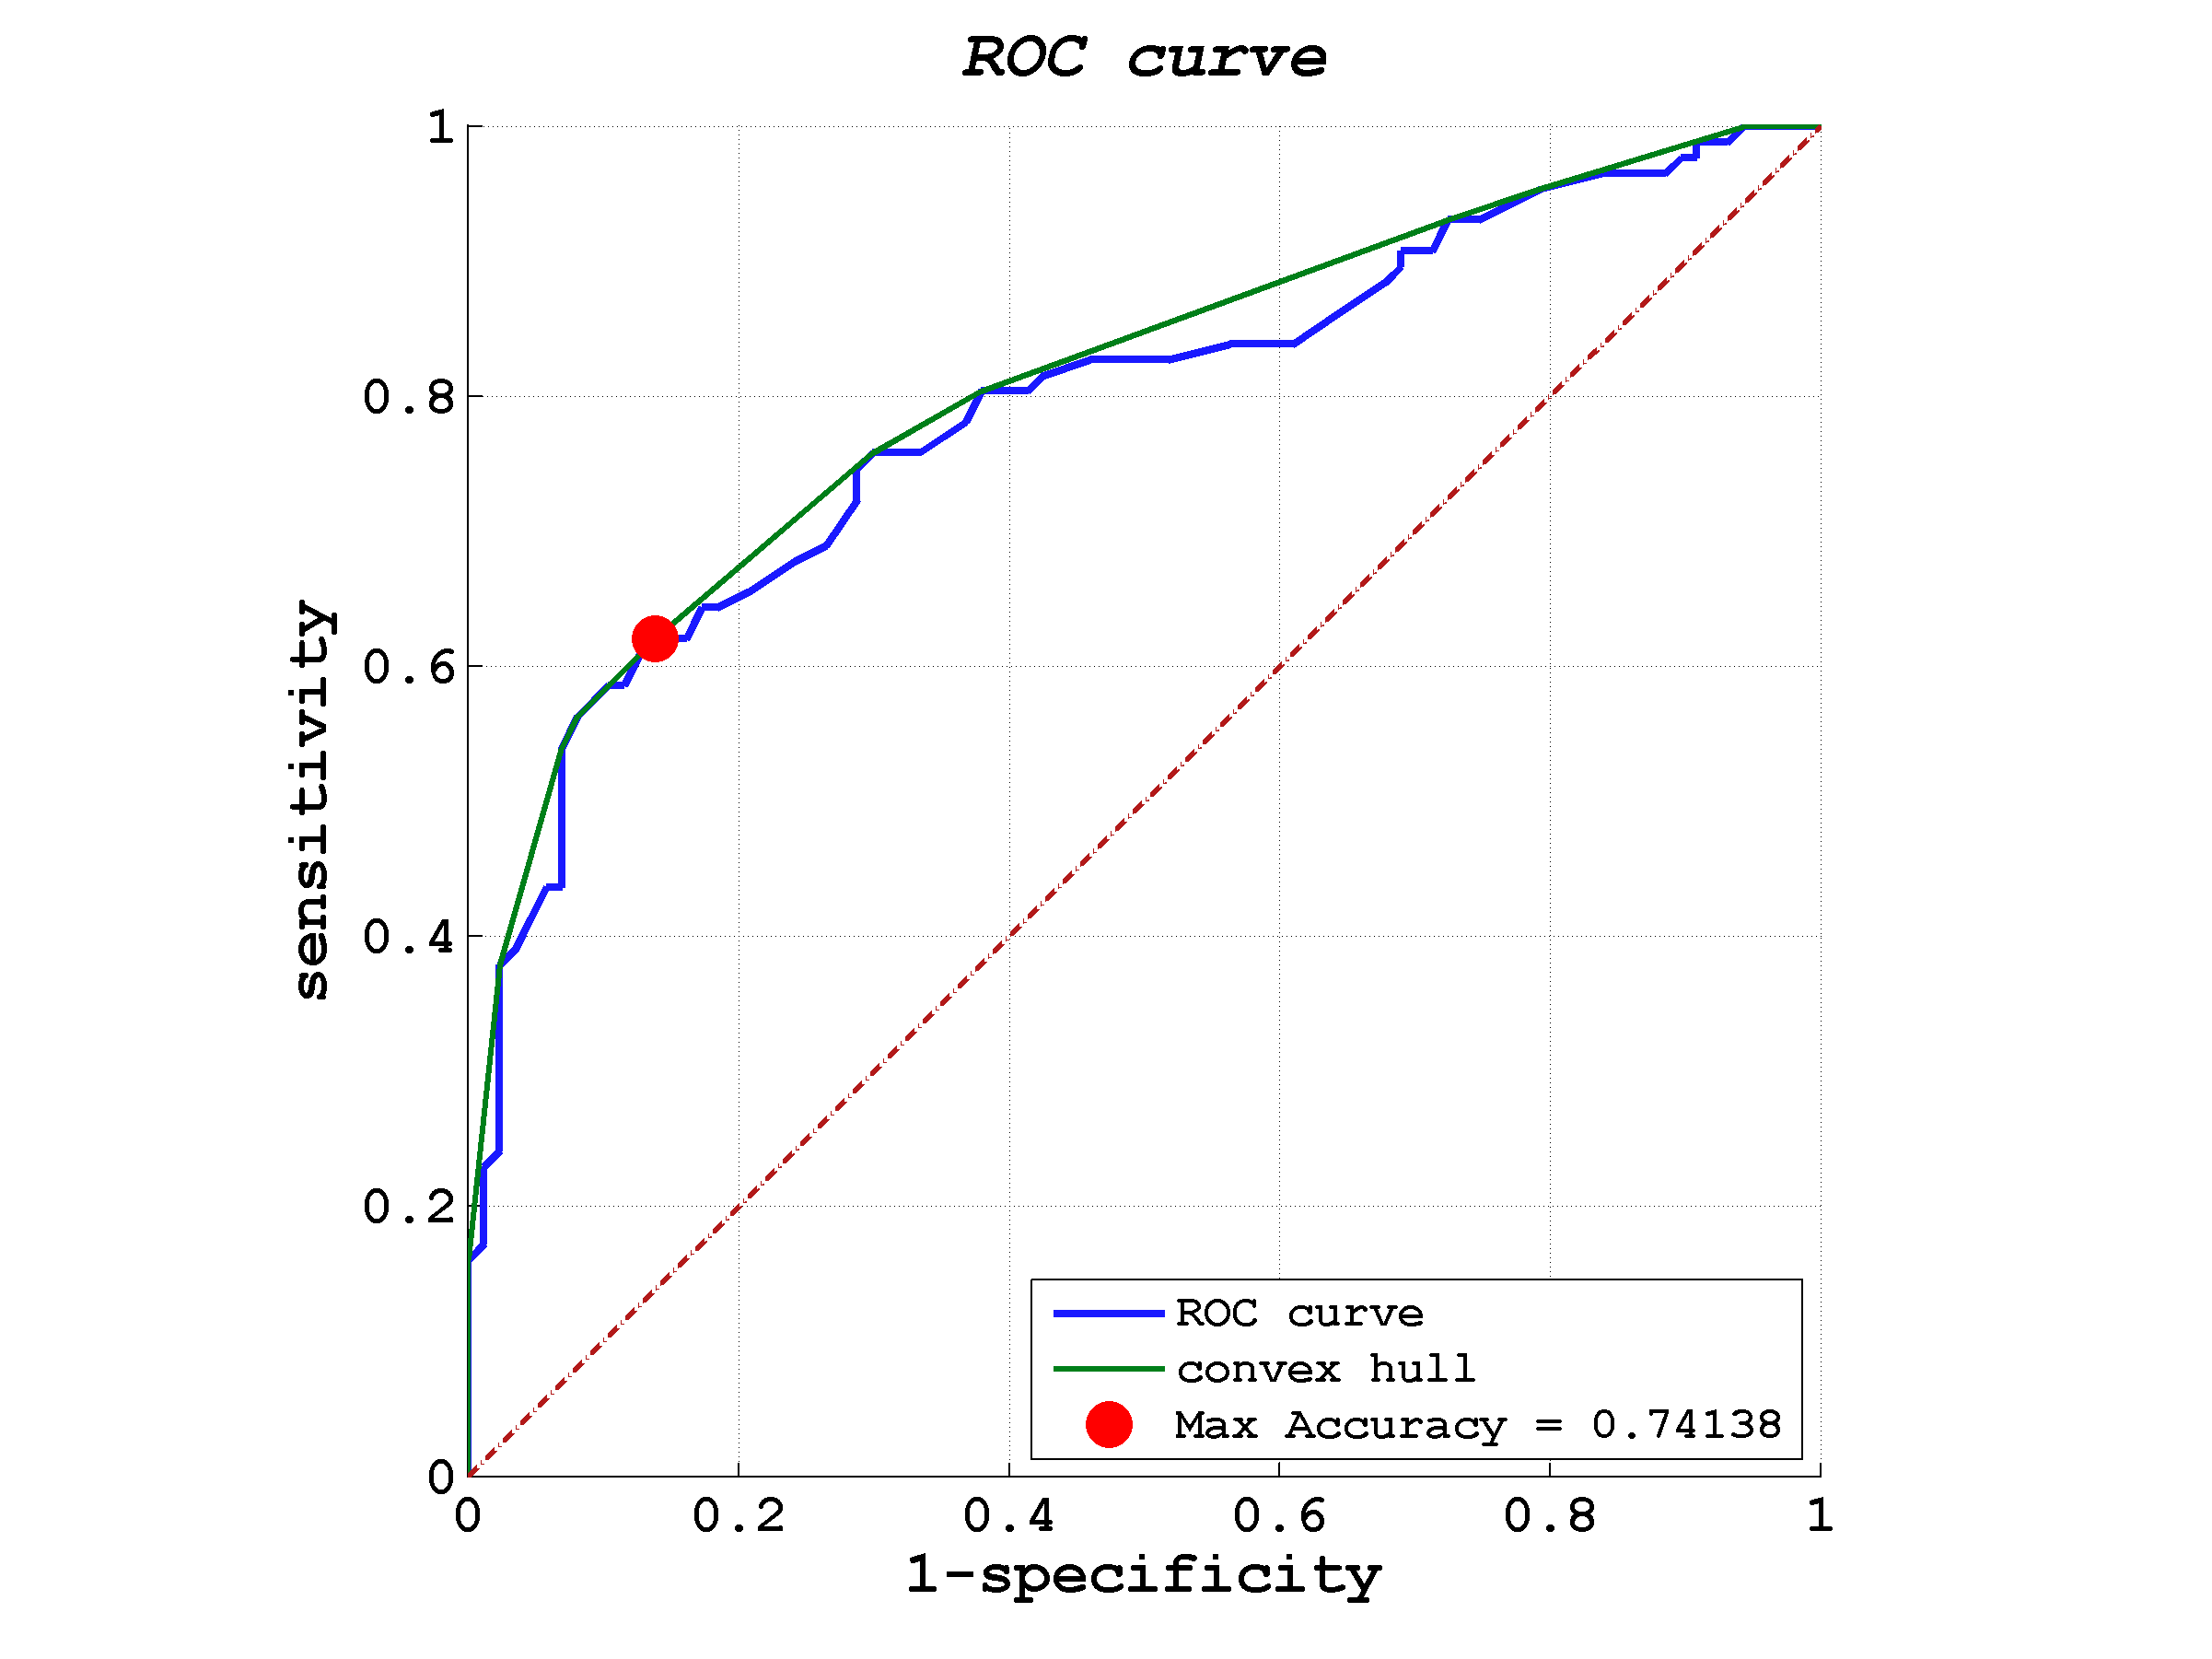
\includegraphics[width=0.46\textwidth]{./images/exp01/SVMprob_MSi_std.png}
      \label{ch6:fig1:a}
    }
    \hspace{1mm}
    \subfigure[SVM norm - ROC]{
      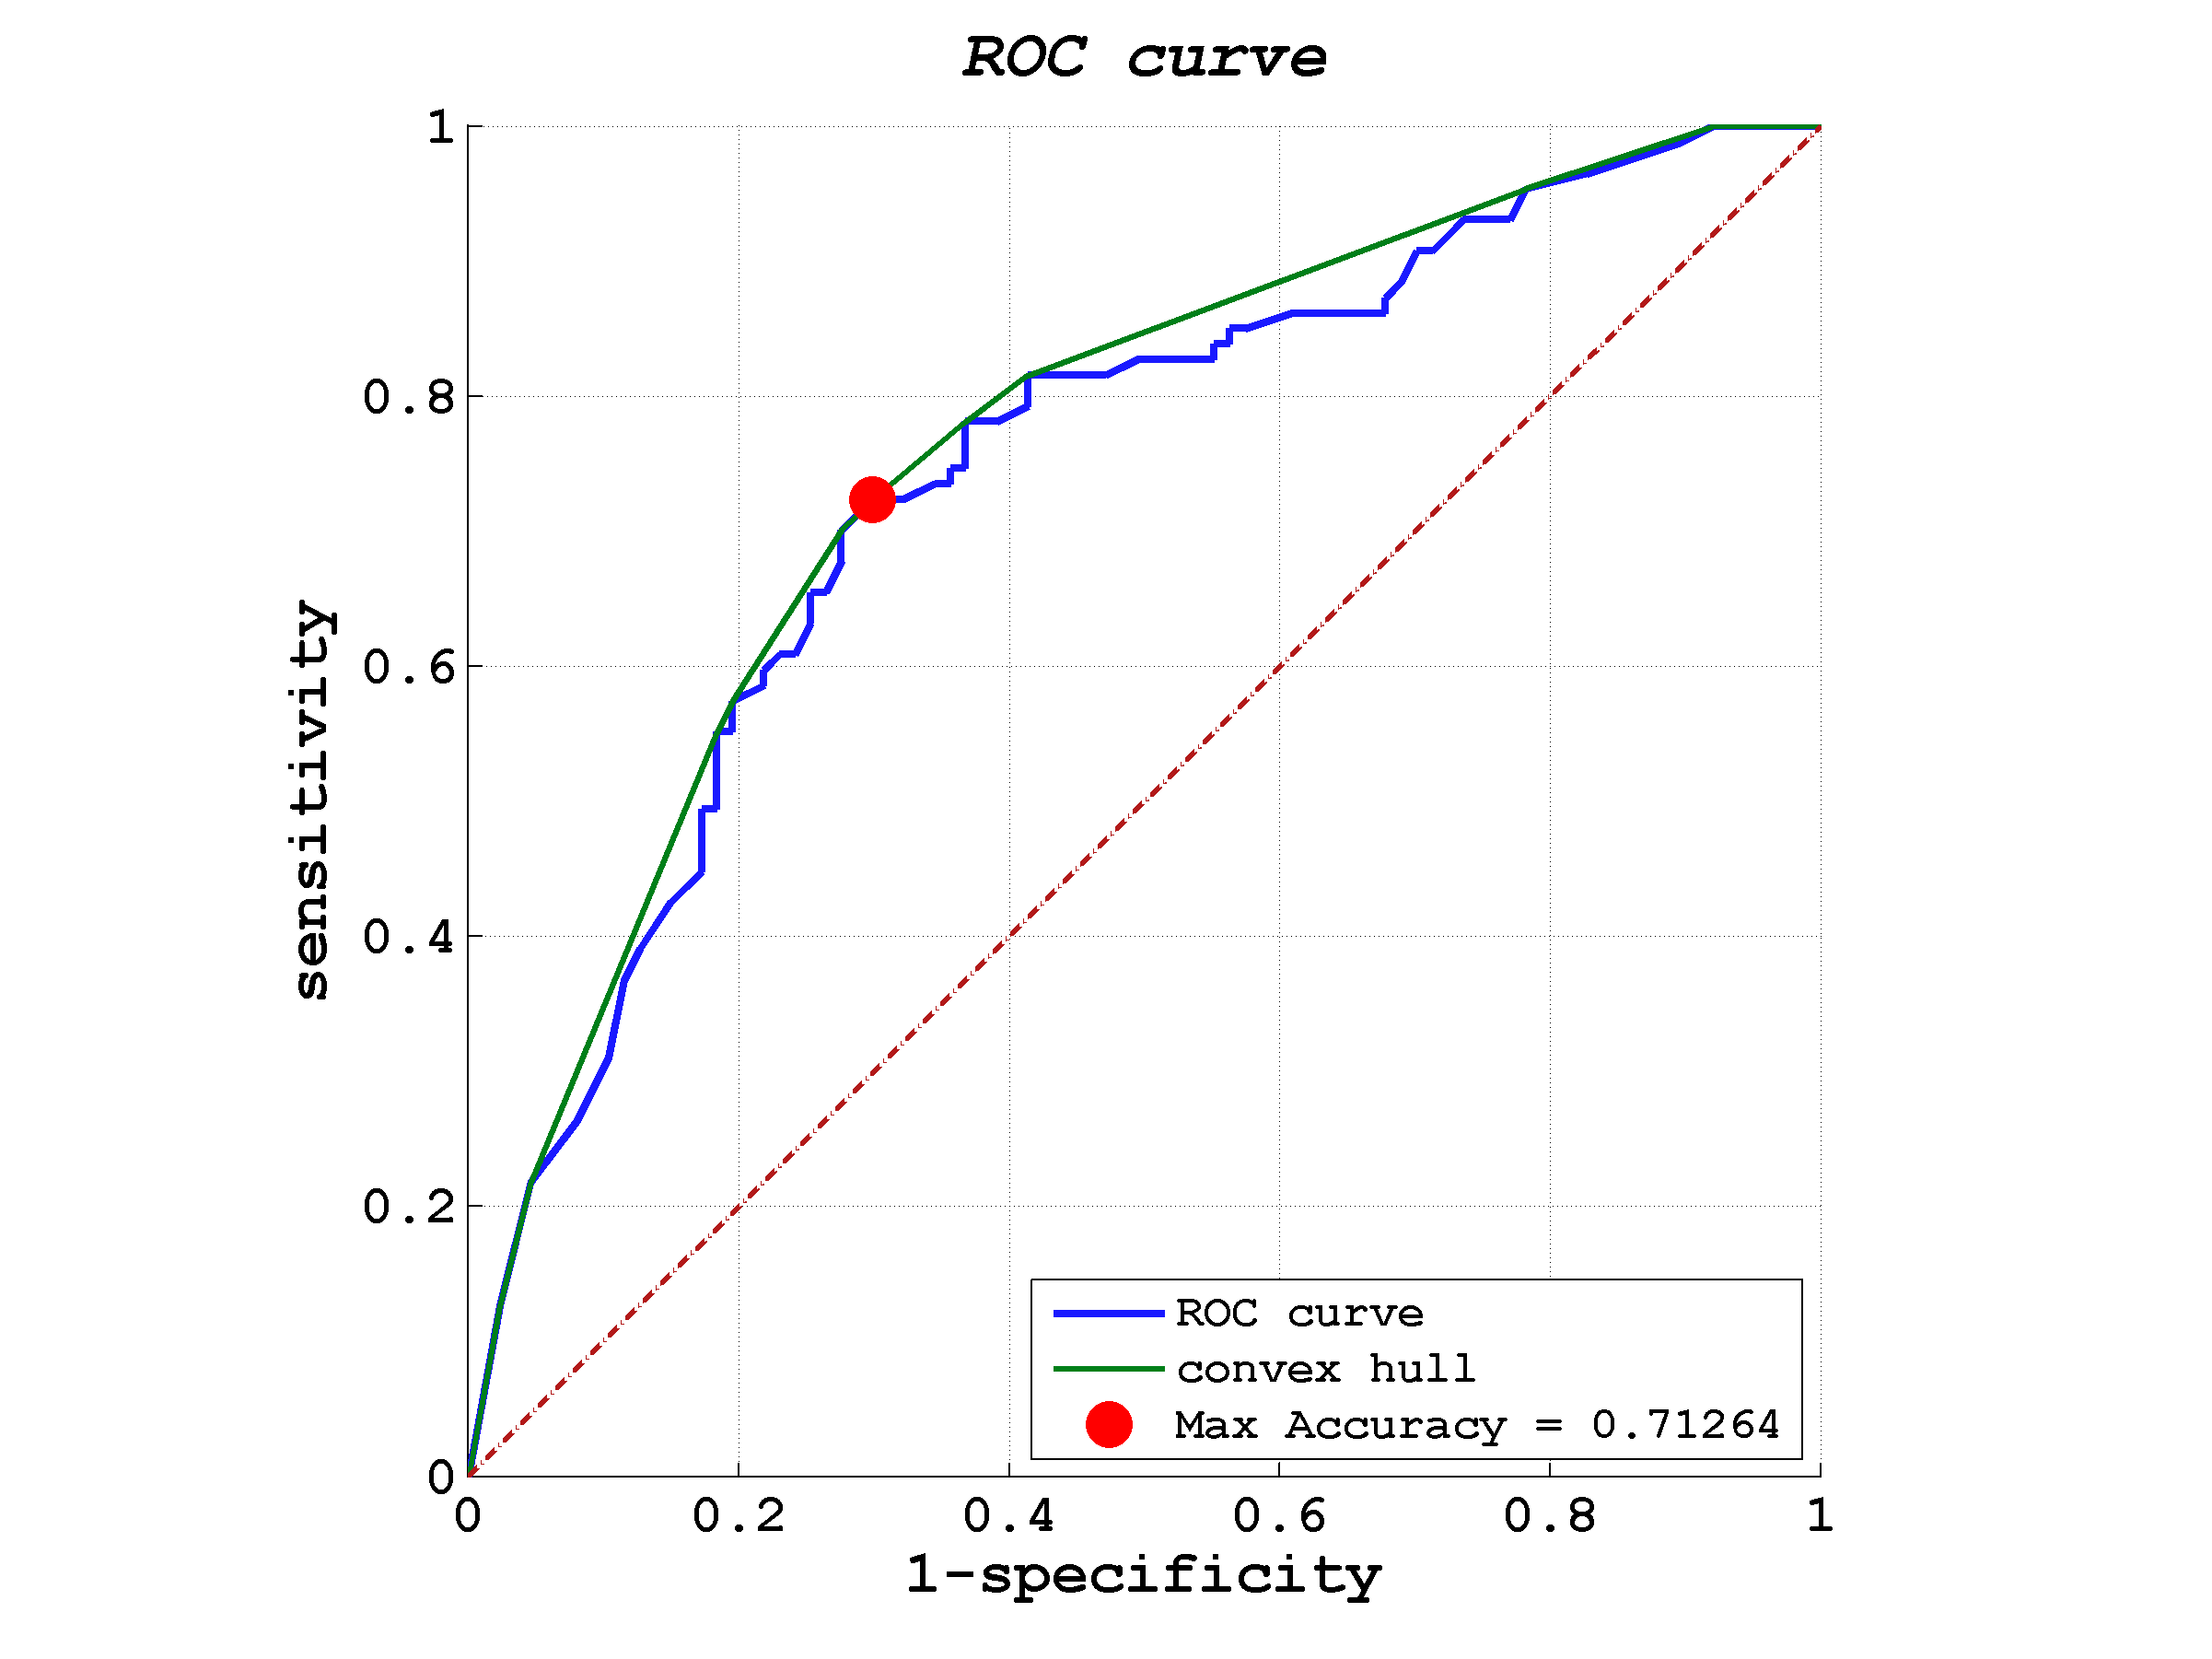
\includegraphics[width=0.46\textwidth]{./images/exp01/SVMprob_MSi_norm.png}
      \label{ch6:fig1:b}
    }
    \\
    \subfigure[RF std - ROC]{
      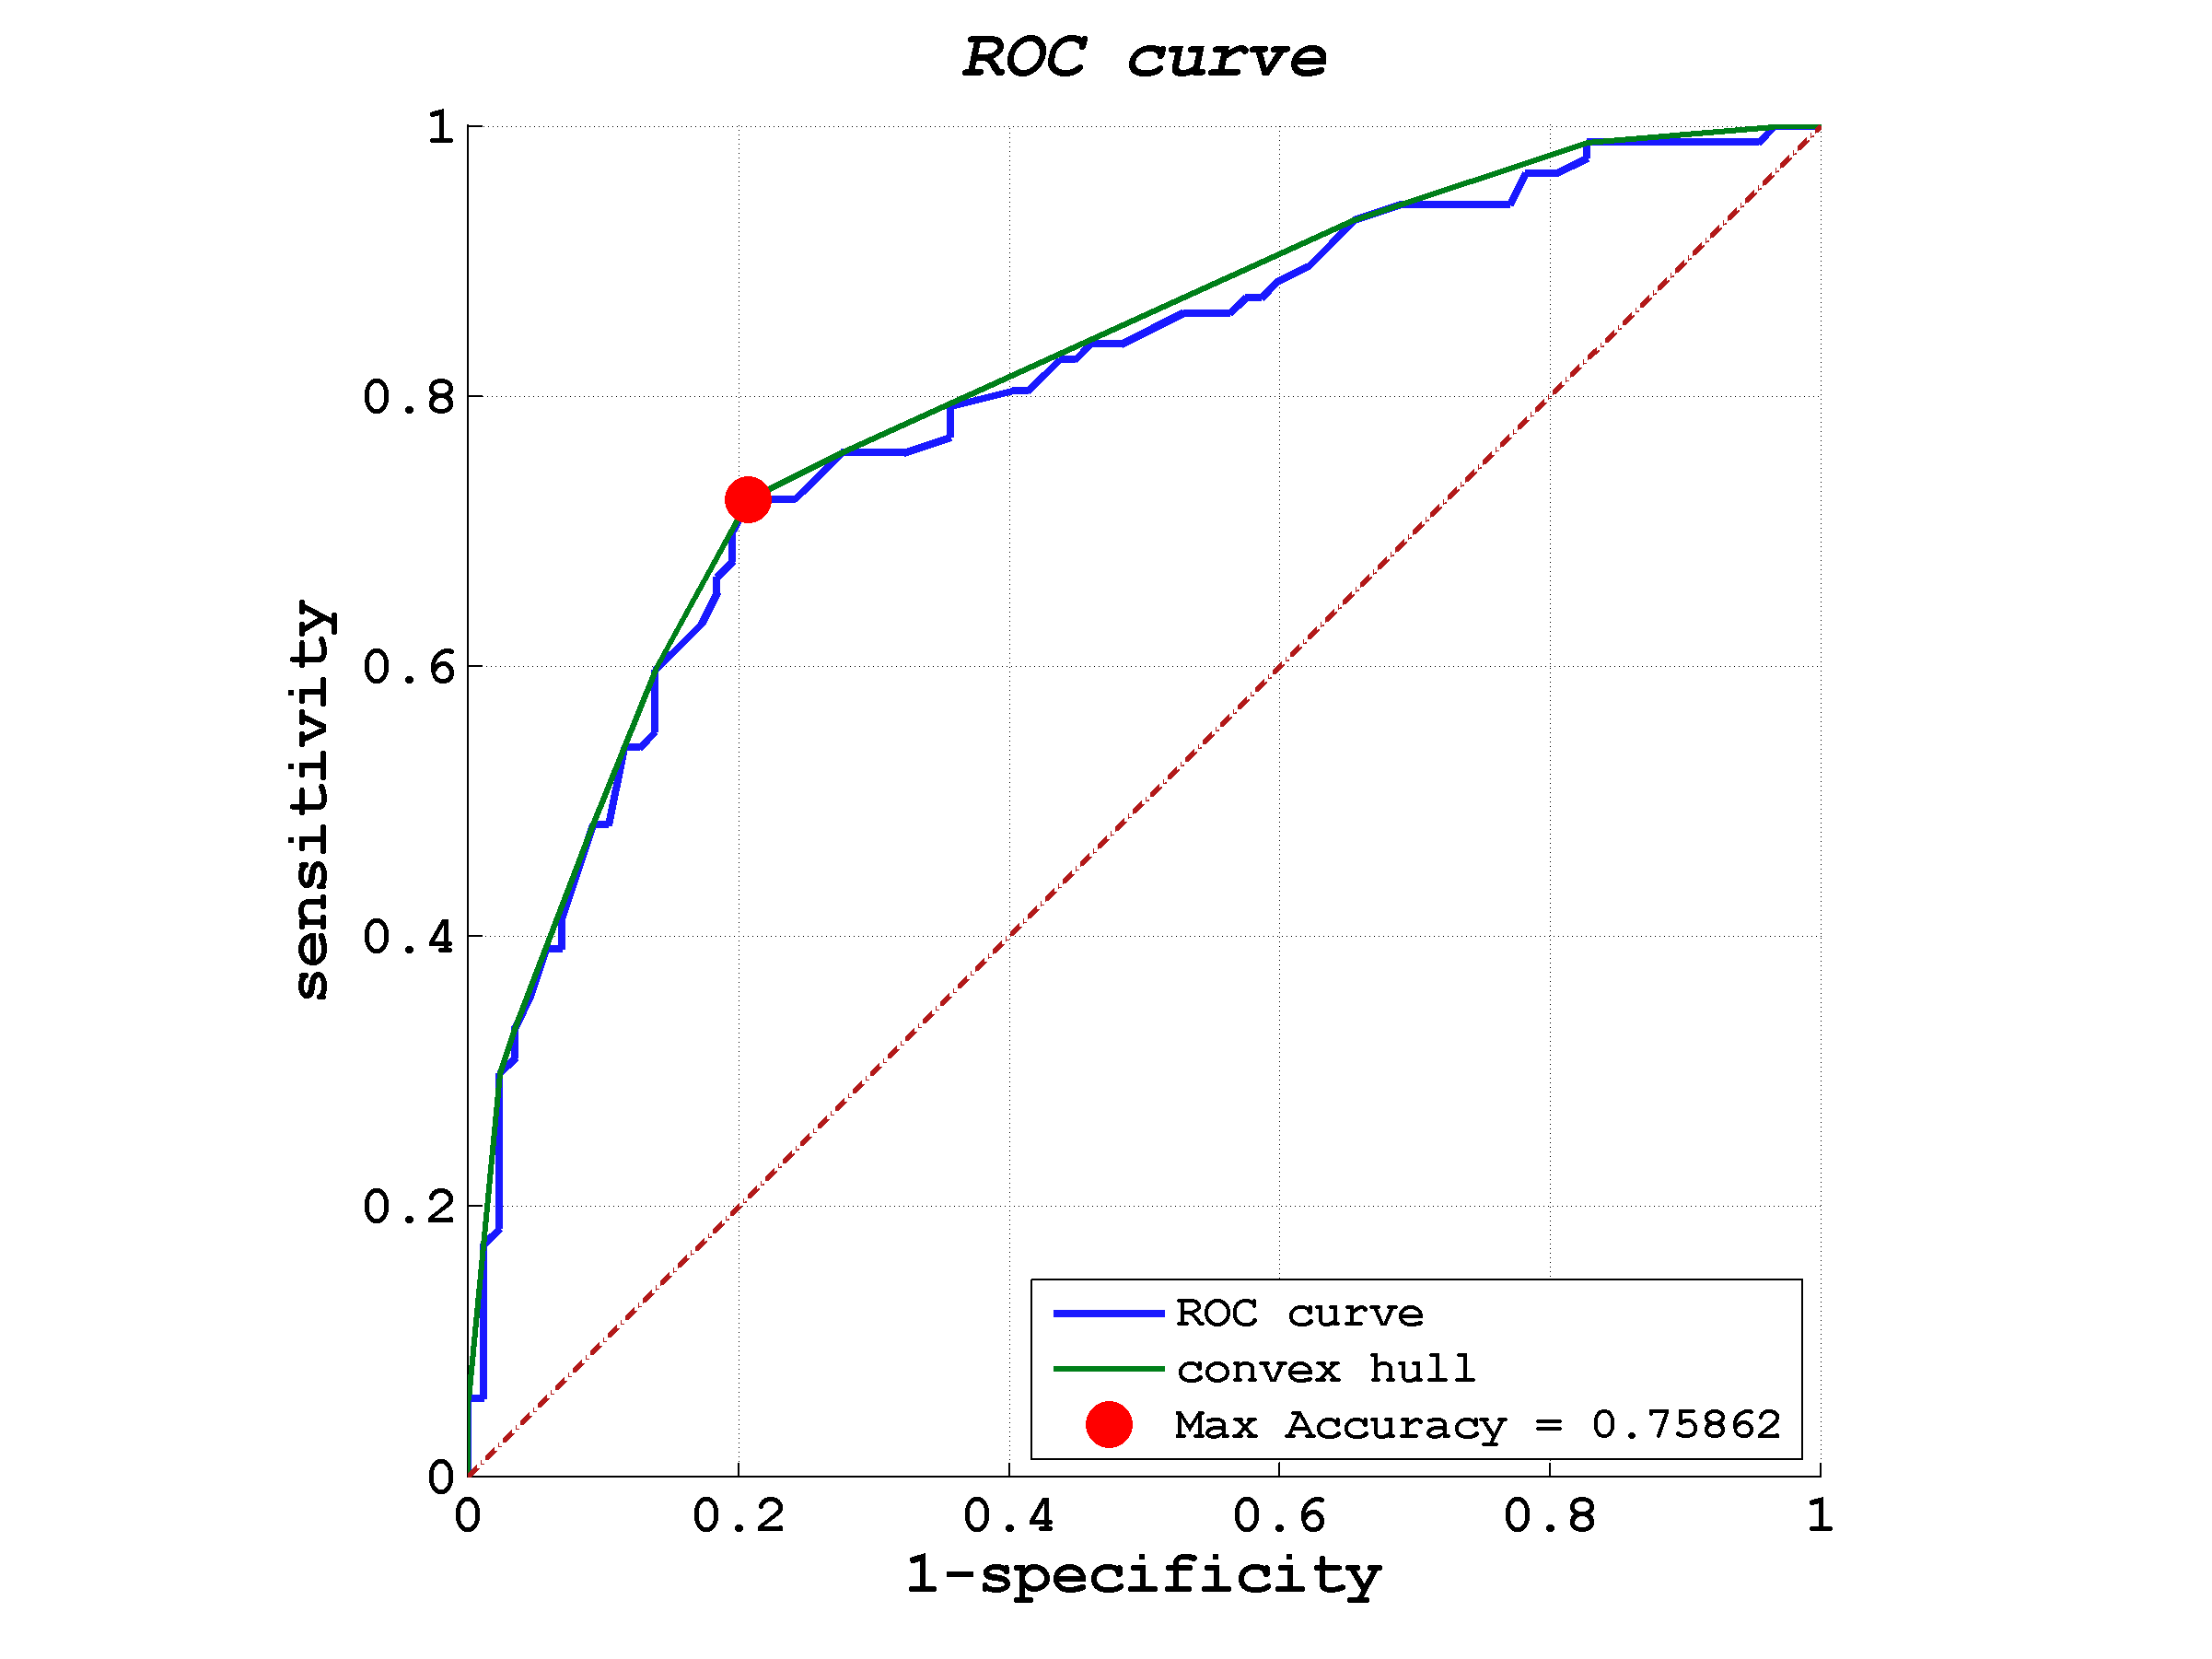
\includegraphics[width=0.46\textwidth]{./images/exp01/RF_MSi_std.png}
      \label{ch6:fig1:c}
    }    
    \hspace{1mm}
    \subfigure[RF std - ROC]{
      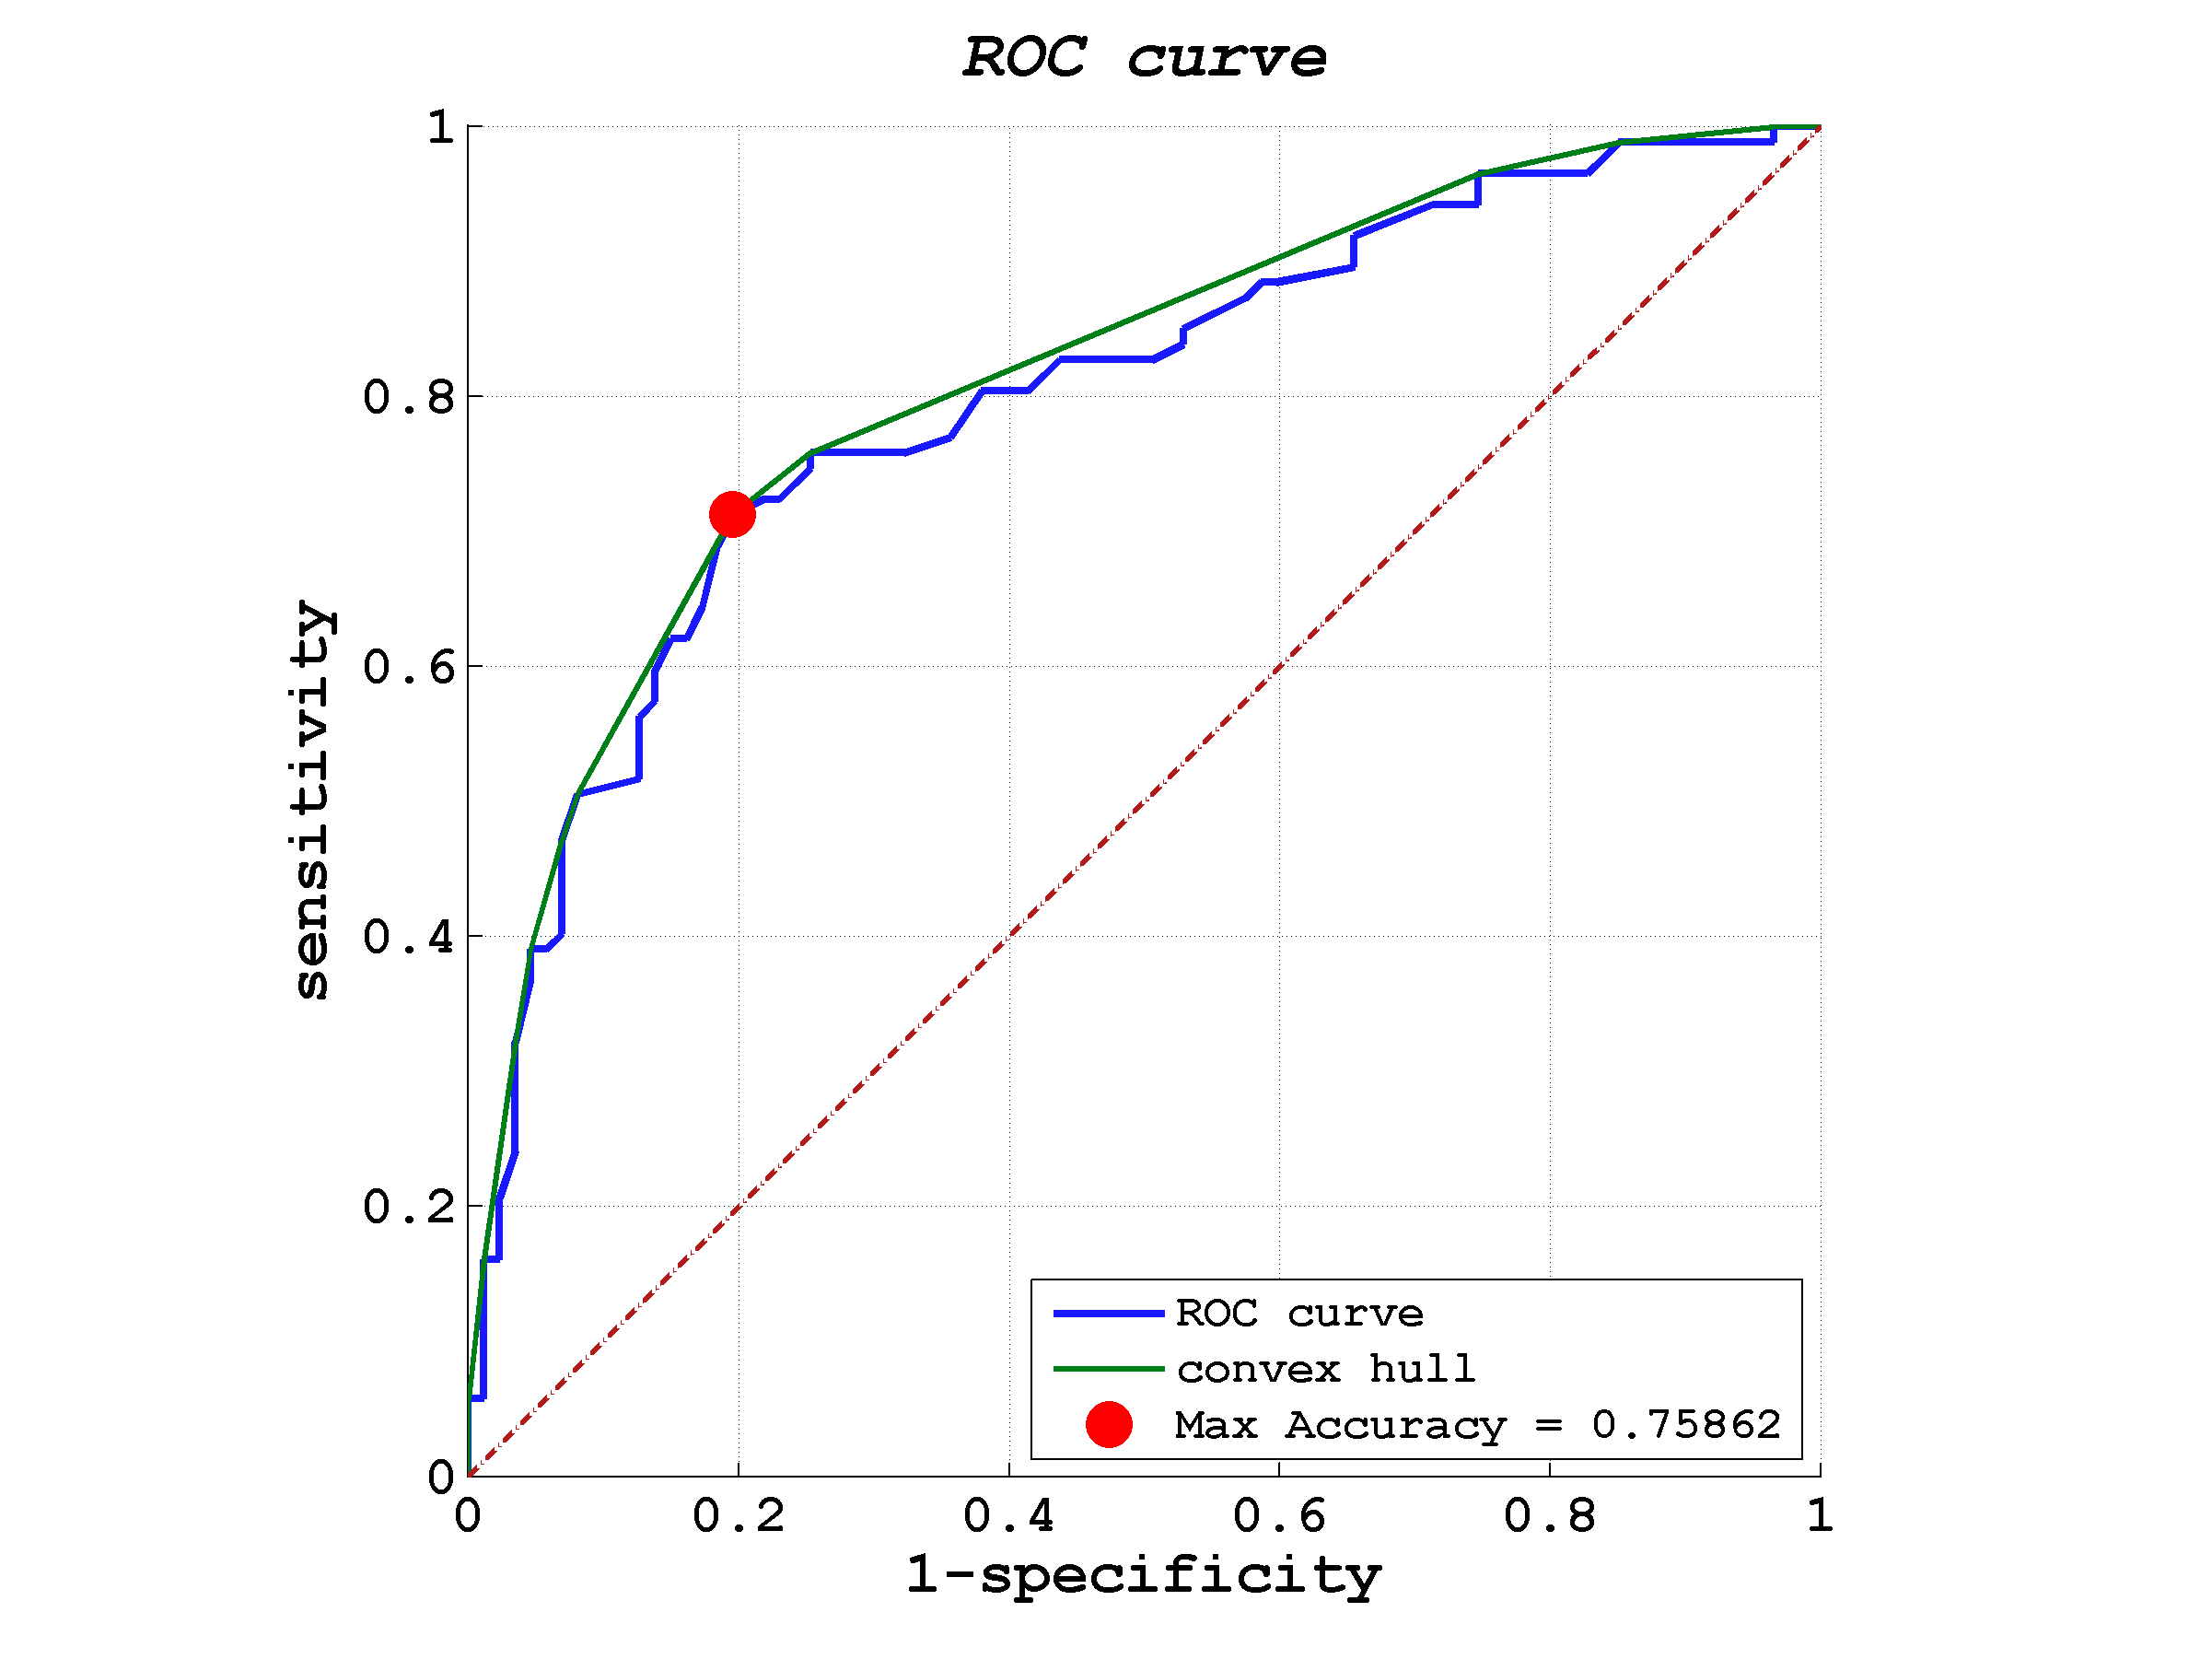
\includegraphics[width=0.46\textwidth]{./images/exp01/RF_MSi_norm.png}
      \label{ch6:fig1:d}
    }
    \caption{ROC curves for \texttt{MSi} features classification}
    \label{ch6:fig1}
\end{figure}

\vspace{0.5cm}

\subsubsection{Features: \texttt{MSiHLV}}

The results of applying normalization to data are different when much more features are involved. For example, in a \texttt{MSiHLV} feature-set (but same results 
have been found for example for \texttt{MSiHUV}), the \Gls{SVM} classifier is unable to find a proper classification with standard features; on the other hand, 
the results are interesting when normalization is applied. Similarly to the previous case (Table \ref{ch6:tab1}), the \Gls{RF} classifier is slightly influenced by
normalization.



\begin{table}[!hbt]
\tiny
 \centering
 \begin{tabularx}{350pt}{ >{\centering\arraybackslash} X |>{\centering\arraybackslash} X |>{\centering\arraybackslash} X |>{\centering\arraybackslash} X |>{\centering\arraybackslash} X |>{\centering\arraybackslash} X |>{\centering\arraybackslash} X}
   Classifier & AUC  & accuracy & precision & F$_1$-Score & sensitivity & specificity \\
   \hline
   \hline
    SVM norm  & 0.87 & 79.89\%  & 74.07\%   & 0.82        & 67.82\%     & 91.95\%  \\
    \hline
    \hline
    RF std    & 0.89 & 81.03\%  & 79.35\%   & 0.82        & 78.16\%     & 83.91\%  \\
    \hline
    RF norm   & 0.90 & 81.61\%  & 77.23\%   & 0.83        & 73.56\%     & 89.66\%  \\
 \end{tabularx}
 \caption{\texttt{MSiHLV} results}
 \label{ch6:tab2}
\end{table}


Table \ref{ch6:tab2} shows the results. The \Gls{ROC} curve of the classifiers is shown in Figure \ref{ch6:fig2}.


\begin{figure}[!htb]
  \centering
    \subfigure[SVM norm - ROC]{
      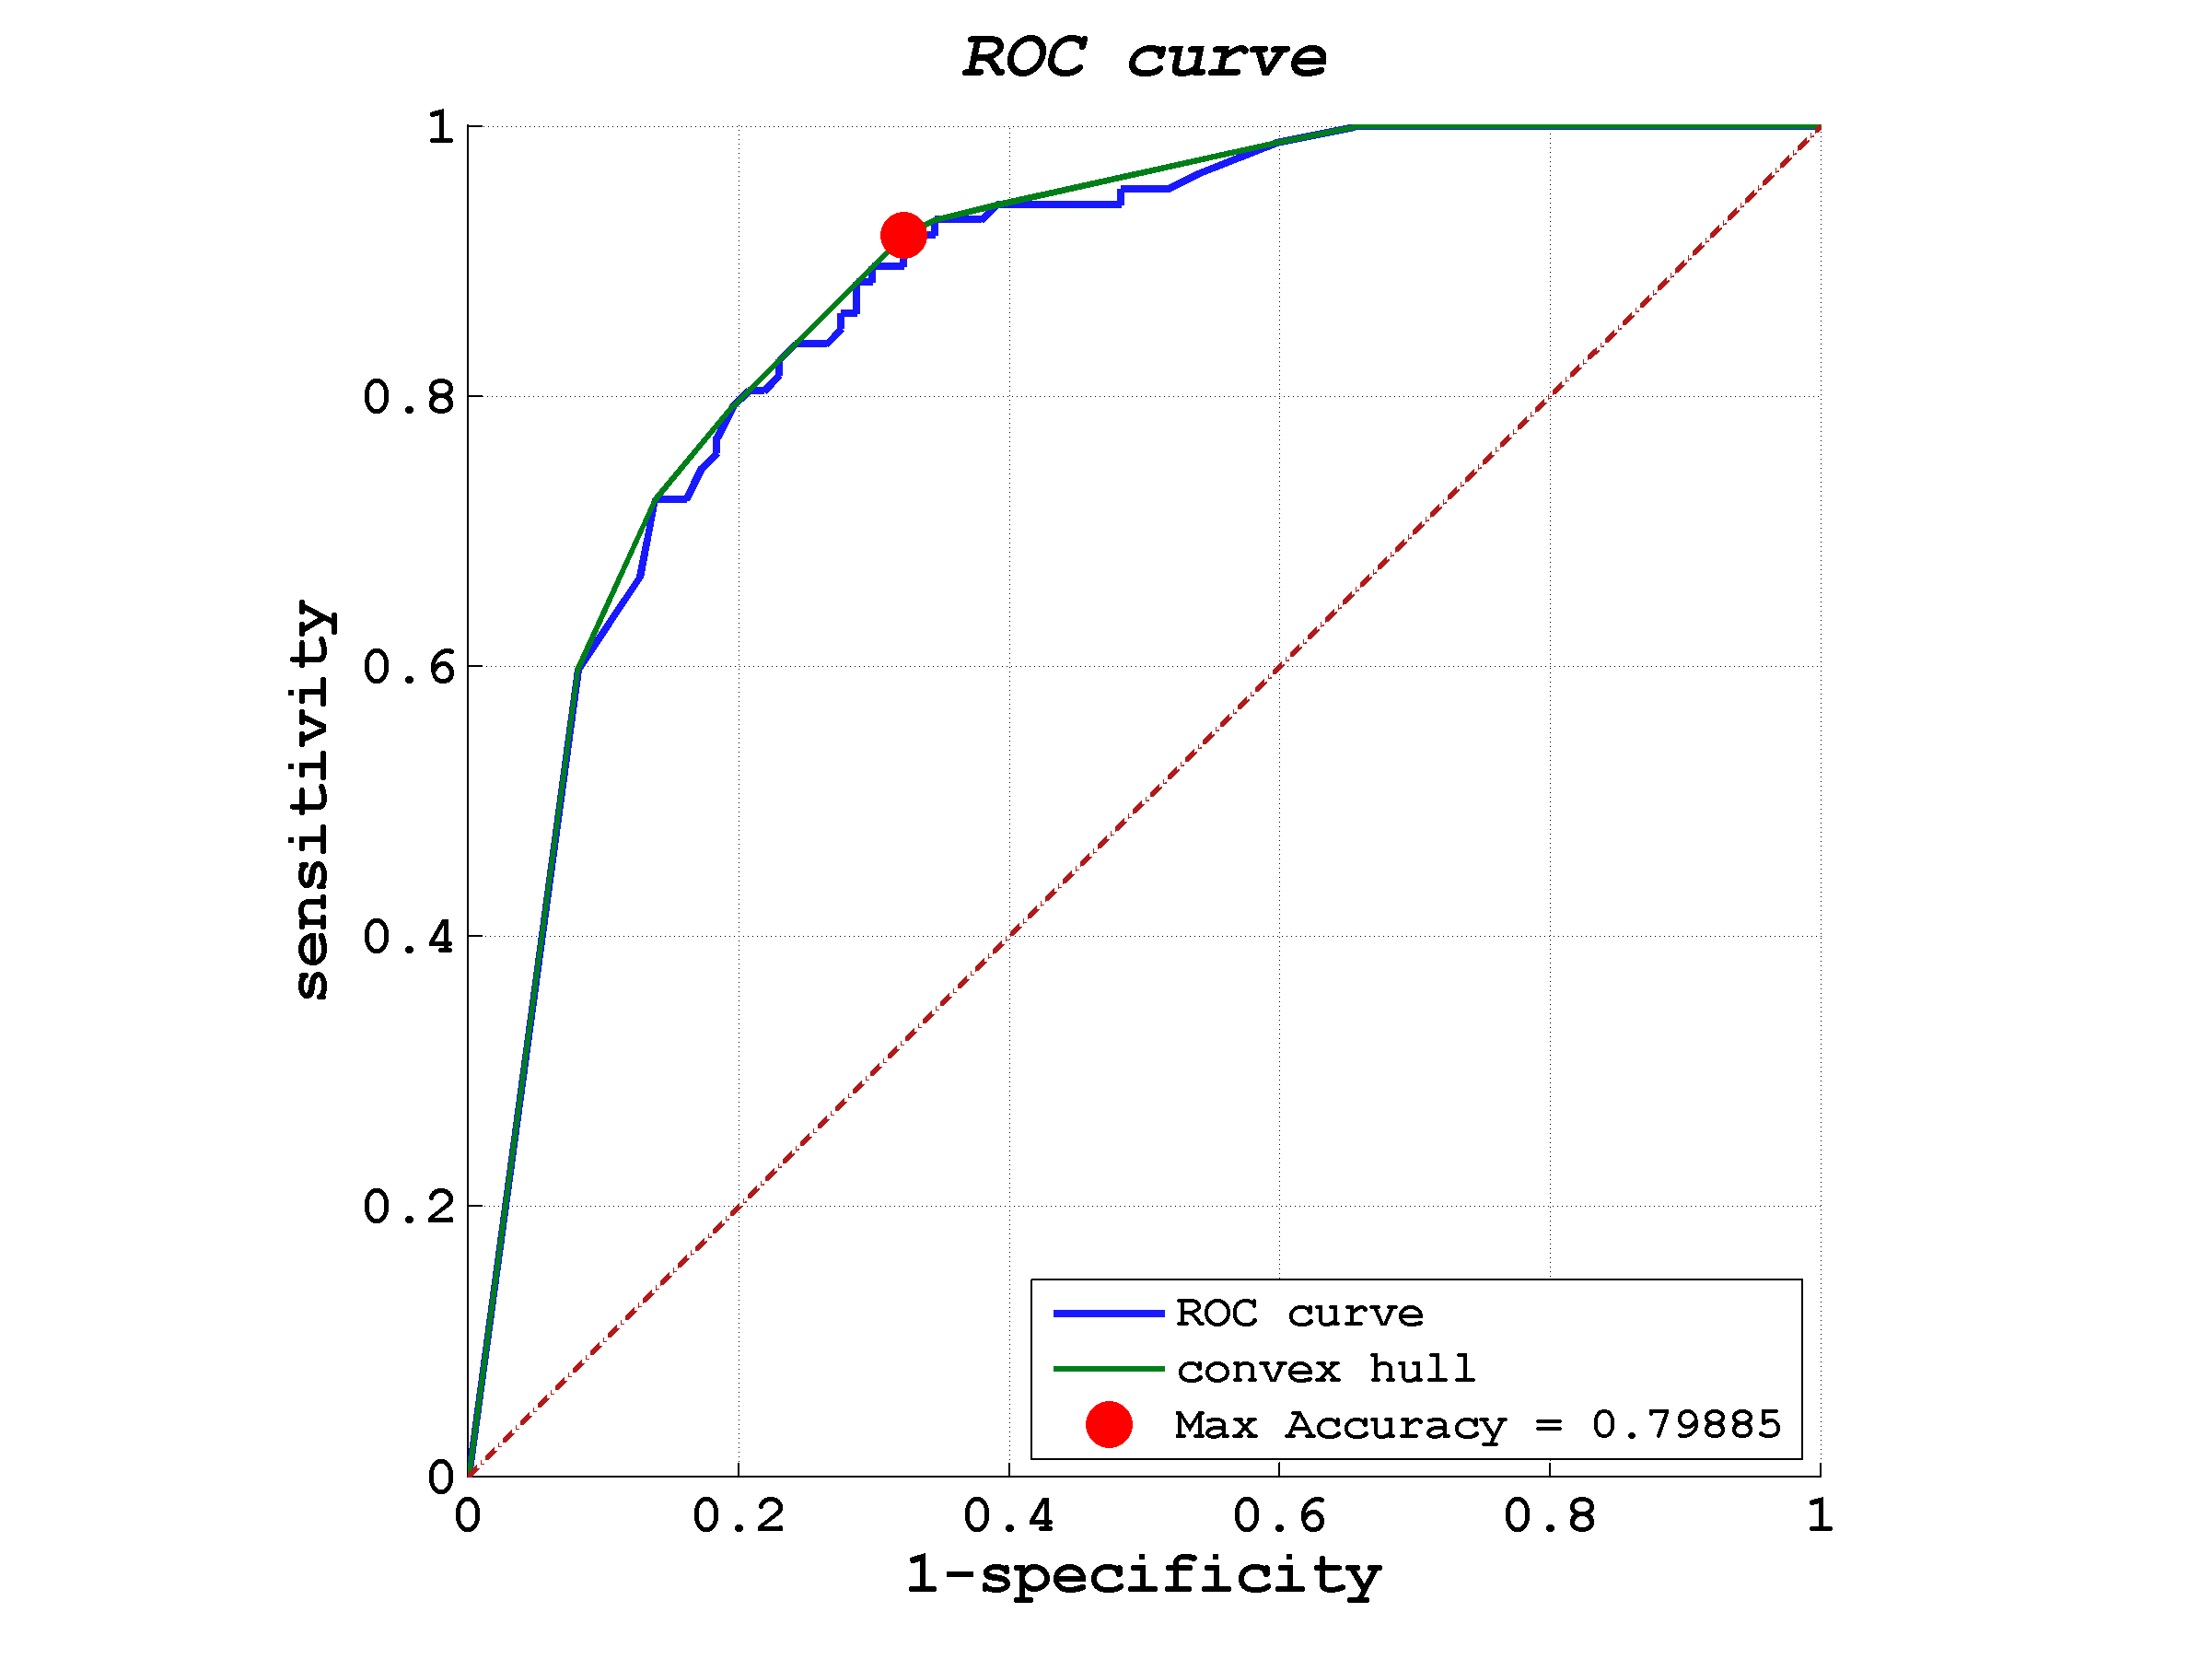
\includegraphics[width=0.46\textwidth]{./images/exp01/SVMprob_MSiHLV_norm.png}
      \label{ch6:fig2:b}
    }
    \\
    \subfigure[RF std - ROC]{
      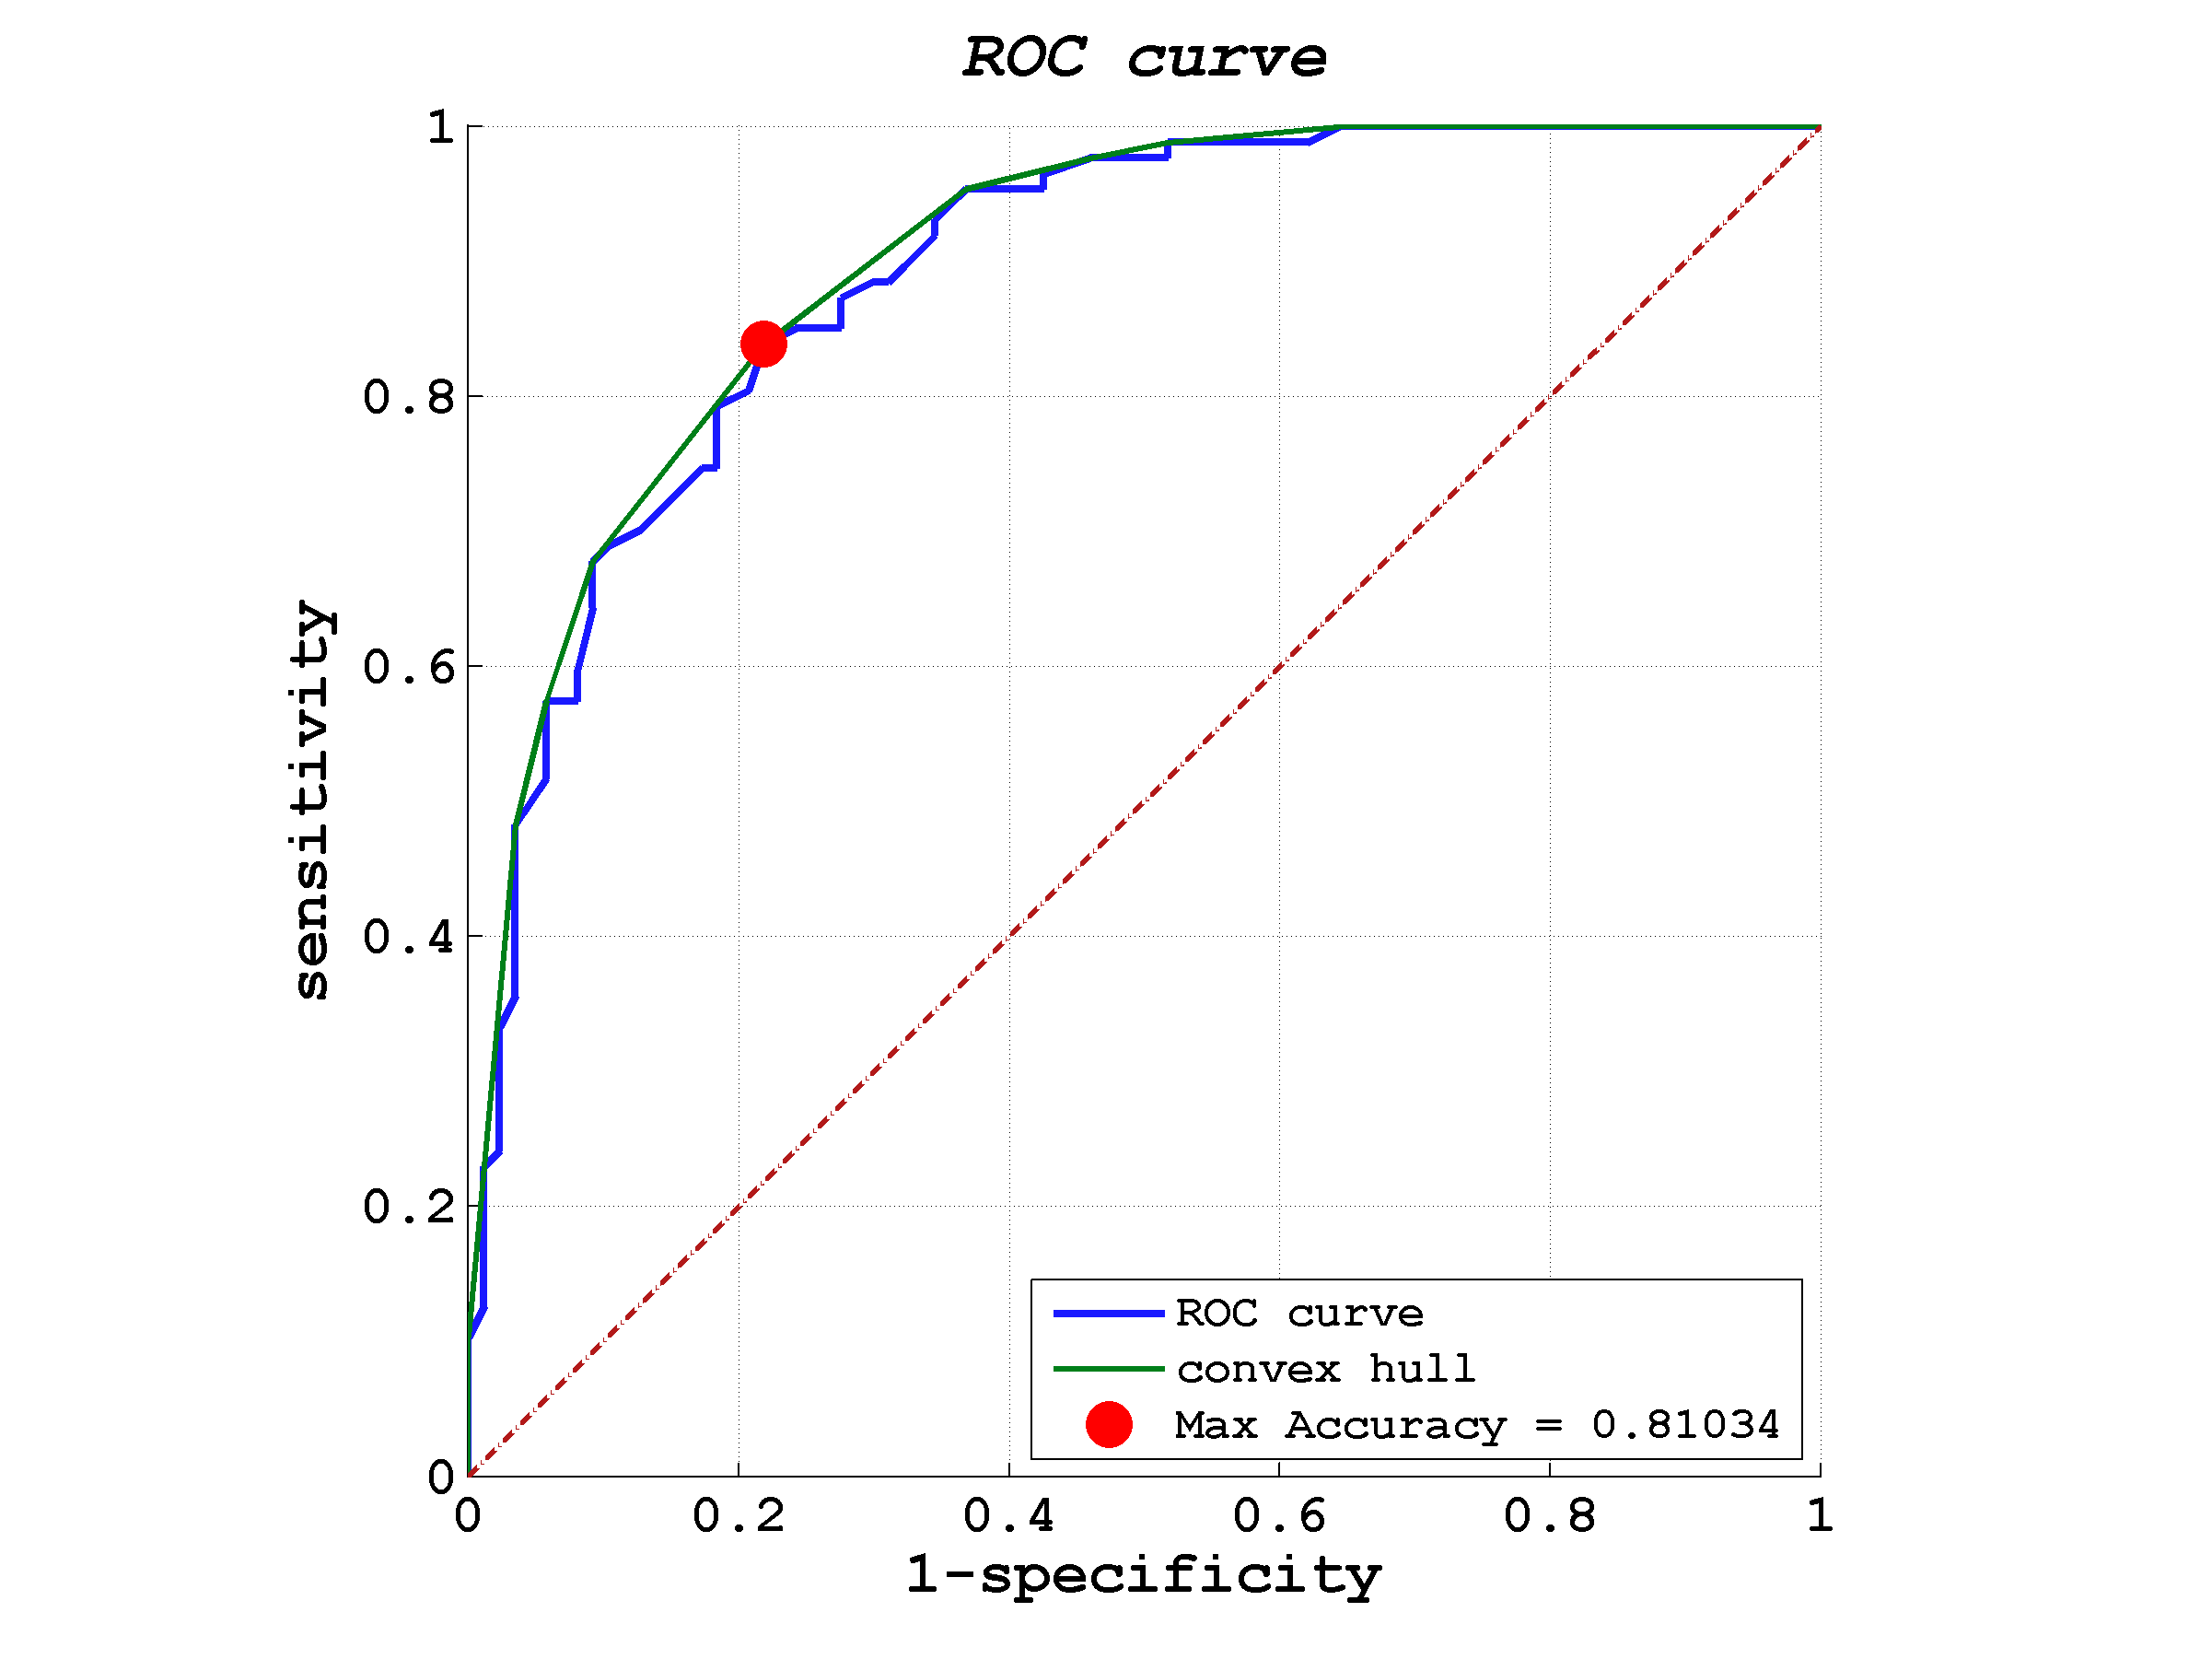
\includegraphics[width=0.46\textwidth]{./images/exp01/RF_MSiHLV_std.png}
      \label{ch6:fig2:c}
    }    
    \hspace{1mm}
    \subfigure[RF std - ROC]{
      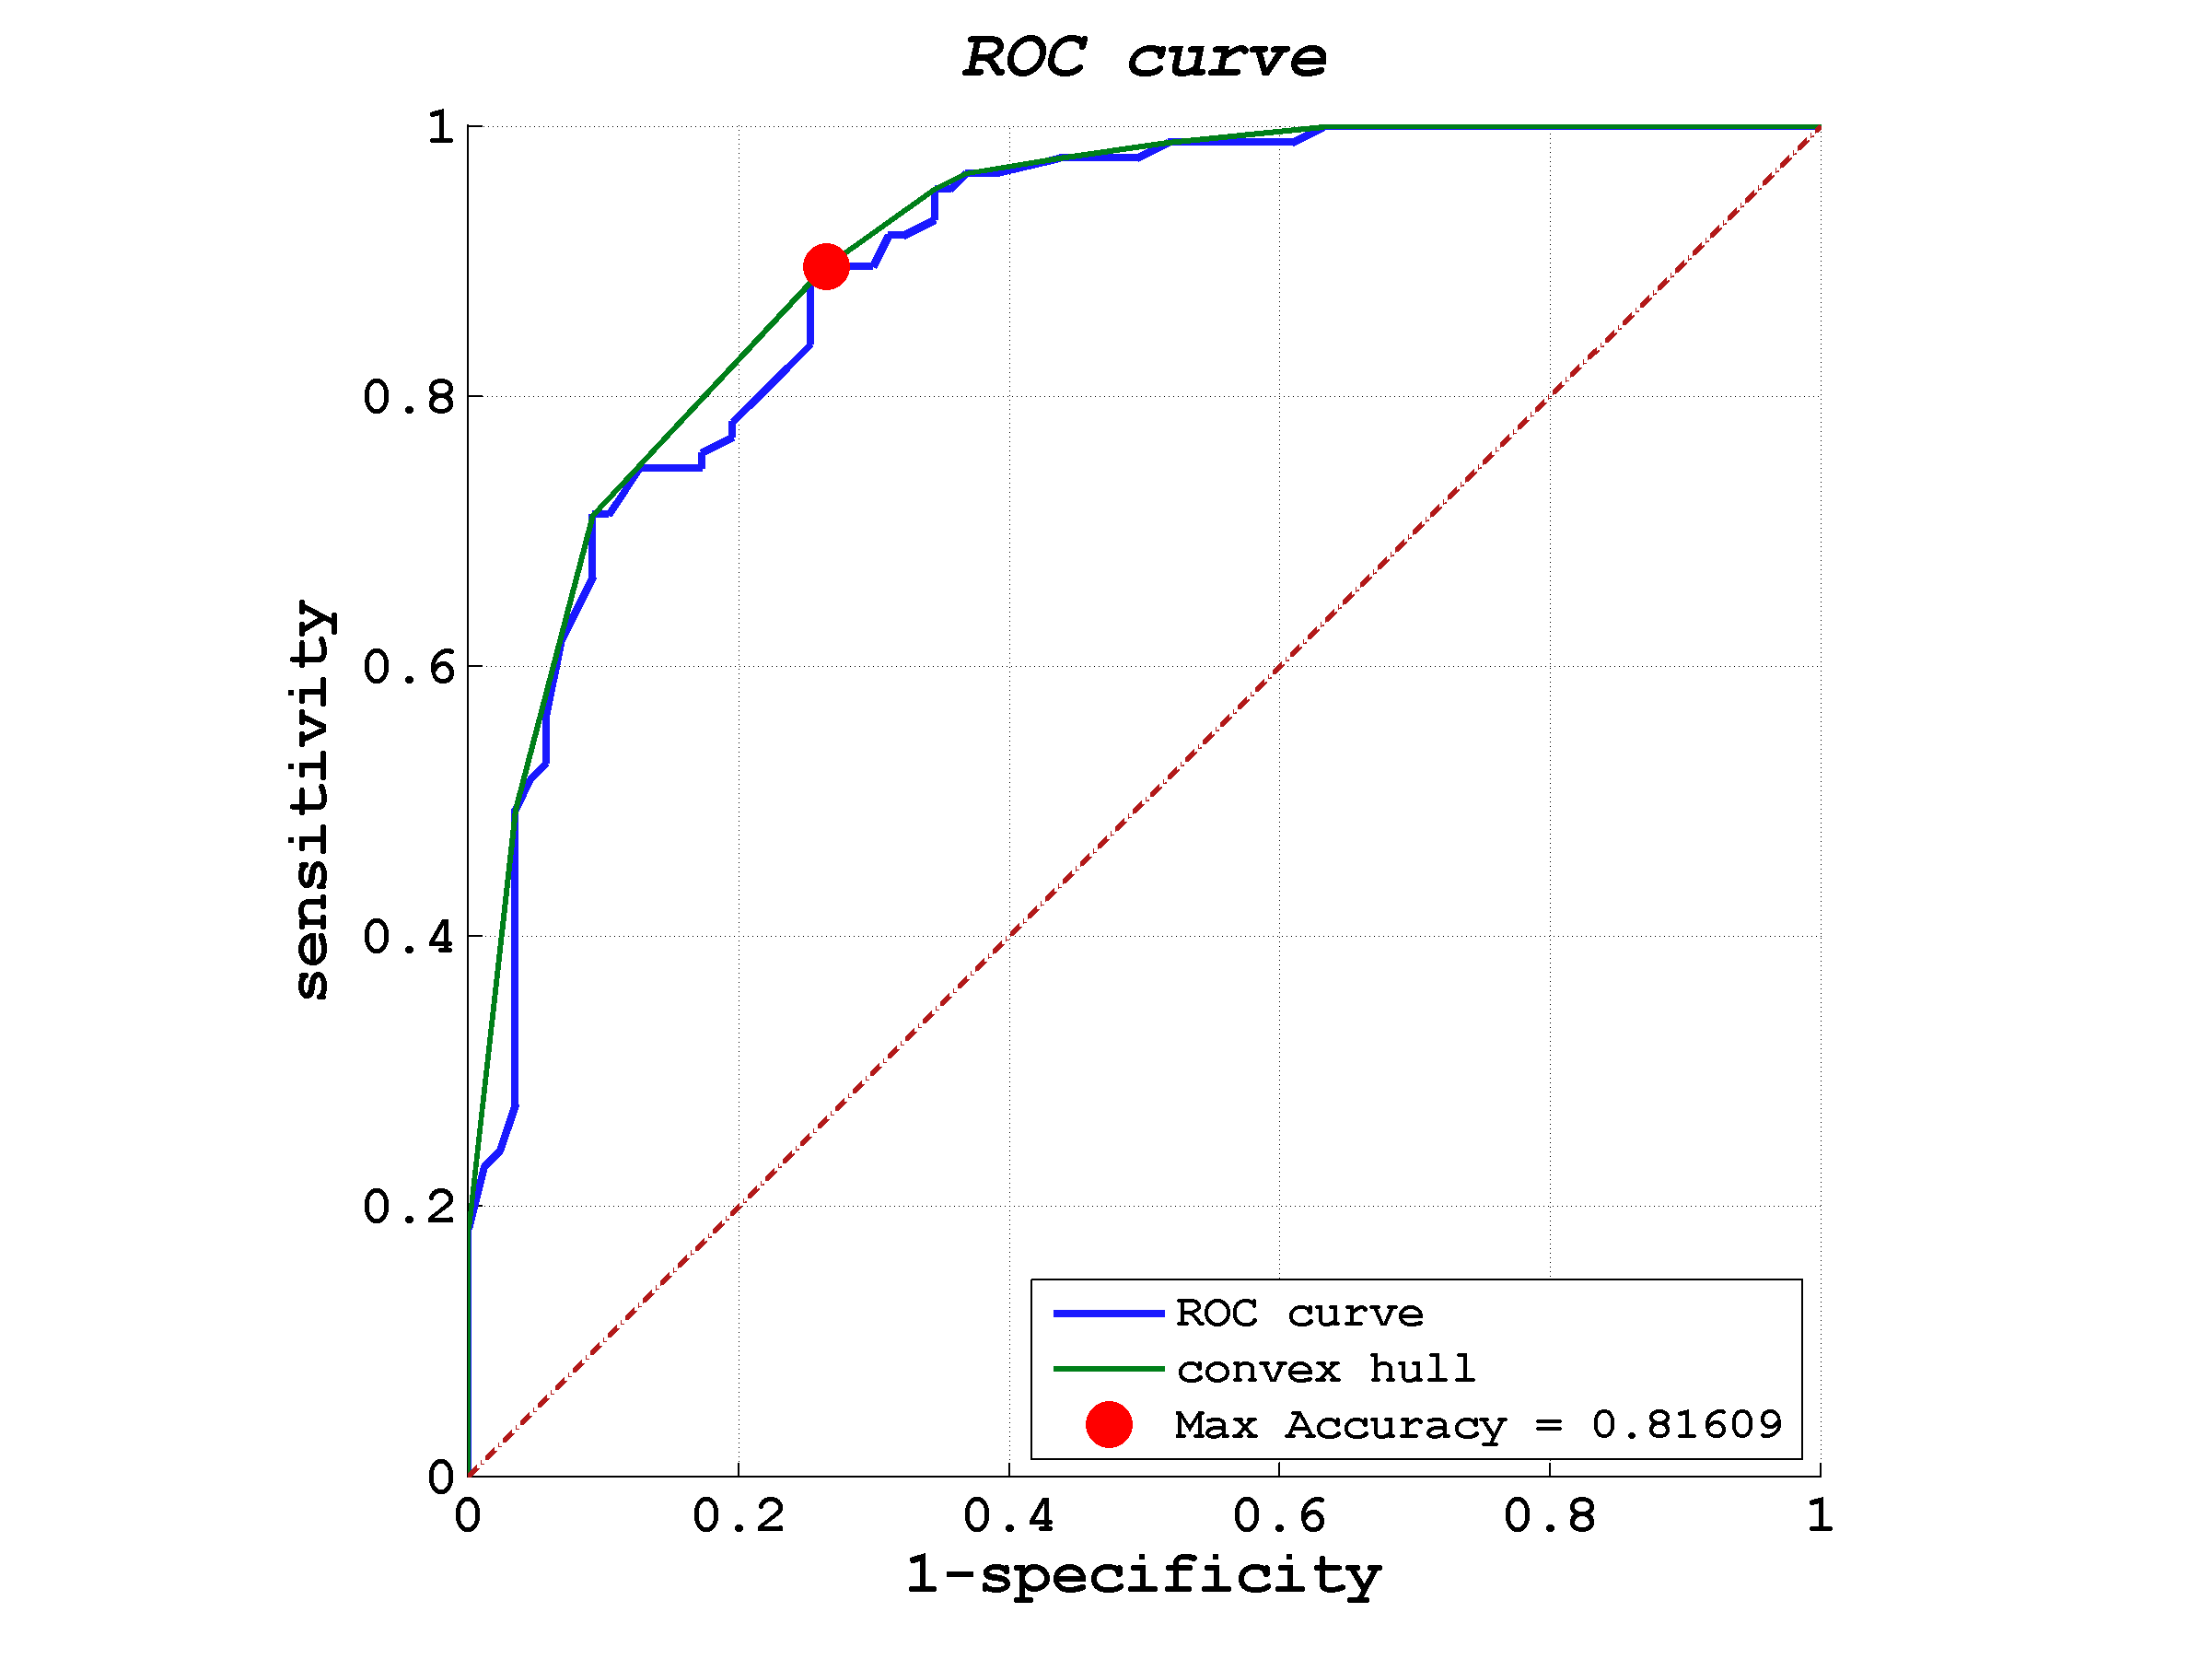
\includegraphics[width=0.46\textwidth]{./images/exp01/RF_MSiHLV_norm.png}
      \label{ch6:fig2:d}
    }
    \caption{ROC curves for \texttt{MSiHLV} features classification}
    \label{ch6:fig2}
\end{figure}


As normalization is generally considered a good practice and as we found, with or experiments, advantages when we applied it to our data, we considered 
only a normalized dataset in all the following experiments.

\vspace{0.5cm}


\subsection{Extended Dataset}

In this experiment we analyzed the effect of considering the extended dataset, as described in Section \ref{ch4:ed}. Rotated and mirrored images should provide some information for
all the features that are orientation dependent, in all the other cases, the added elements are just replicates of already present instances.
Also in this case we run test with different sets of features.
\\
The Matlab code implemented to run \textit{experiment 2} is listed in \ref{appendixB:exp2}


\vspace{0.5cm}

\subsection{Extended Dataset: Experimental Results}

We considered three different ways of extending our dataset, resulting in four different experiments:

\begin{itemize}
 \item no dataset is extended (abbreviated with \textit{default}),
 \item the \textit{train} dataset is extended (abbreviated with \textit{ext-T}),
 \item the \textit{evaluation} dataset is extended (abbreviated with \textit{ext-E}),
 \item both dataset are extended (abbreviated with \textit{ext-A}). 
\end{itemize}

We expected some advantages in extending the dataset when orientation-dependent features are involved. On the other hand,
growing the dataset too much could bring in much more noise than useful information, resulting in a worse performance of the classifier.
When the evaluation dataset is extended, the classification value of an image is the average of the classification of the derived images (see Section \ref{ch4:ed}).
We report here the most significant experiments and results.

\vspace{0.5cm}

\subsubsection{Features: \texttt{MSiHU} - classifier: SVM}

We applied our \Gls{SVM} classifier to the feature-set coded \texttt{MSiHU}, please note that feature \texttt{U} is orientation dependent. The results are the following:


\begin{table}[!hbt]
\tiny
 \centering
 \begin{tabularx}{350pt}{ >{\centering\arraybackslash} X |>{\centering\arraybackslash} X |>{\centering\arraybackslash} X |>{\centering\arraybackslash} X |>{\centering\arraybackslash} X |>{\centering\arraybackslash} X |>{\centering\arraybackslash} X}
   Classifier     & AUC  & accuracy & precision & F$_1$-Score & sensitivity & specificity \\
   \hline
   \hline
    SVM def.      & 0.86 & 79.89\% &  80.23\% &   0.80 &  80.46\% & 79.31\%  \\
    \hline
    SVM ext-T     & 0.87 & 81.03\% &  80.00\% &   0.81 &  79.31\% & 82.76\%  \\
    \hline
    SVM ext-E     & 0.87 & 81.61\% &  85.71\% &   0.80 &  87.36\% & 75.86\%  \\
    \hline
    SVM ext-A     & 0.88 & 81.61\% &  80.22\% &   0.82 &  79.31\% & 83.91\% \\
 \end{tabularx}
 \caption{\texttt{MSiHU} results (SVM)}
 \label{ch6:tab3}
\end{table}

  
More in detail, the number of classified images at optimal threshold is the following:


\begin{table}[!hbt]
\tiny
 \centering
 \begin{tabularx}{320pt}{ >{\centering\arraybackslash} X |>{\centering\arraybackslash} X |>{\centering\arraybackslash} X |>{\centering\arraybackslash} X |>{\centering\arraybackslash} X }
   Classifier     & TP  & FN & TN & FP  \\
   \hline
   \hline
    SVM def.      & 69 & 18 & 70 & 17  \\
    \hline
    SVM ext-T     & 72 & 15 & 69 & 18  \\
    \hline
    SVM ext-E     & 66 & 21 & 76 & 11  \\
    \hline
    SVM ext-A     & 73 & 14 & 69 & 18 \\
 \end{tabularx}
 \caption{\texttt{MSiHU} classified images(SVM)}
 \label{ch6:tab4}
\end{table}  
  
Looking at Table \ref{ch6:tab4}, the number of \Glspl{TP} shows an interesting trend. Extending the \textit{train} dataset improves the classification performance of \Glspl{TP},
worsening the number of \Glspl{TN} of just a unit. It appears that an extended dataset brings some more information. When the only \textit{evaluation} dataset is extended,
the number of \Glspl{TP} lowers considerably, meaning that the training set lacks some information to classify mitoses. On the other hand, the number of \Glspl{TN} is at top.
The overall best performance is found when both datasets are extended.
The \Gls{ROC} curves of this classification is shown in Figure \ref{ch6:fig3}.

\begin{figure}[!htb]
  \centering
    \subfigure[SVM default - ROC]{
      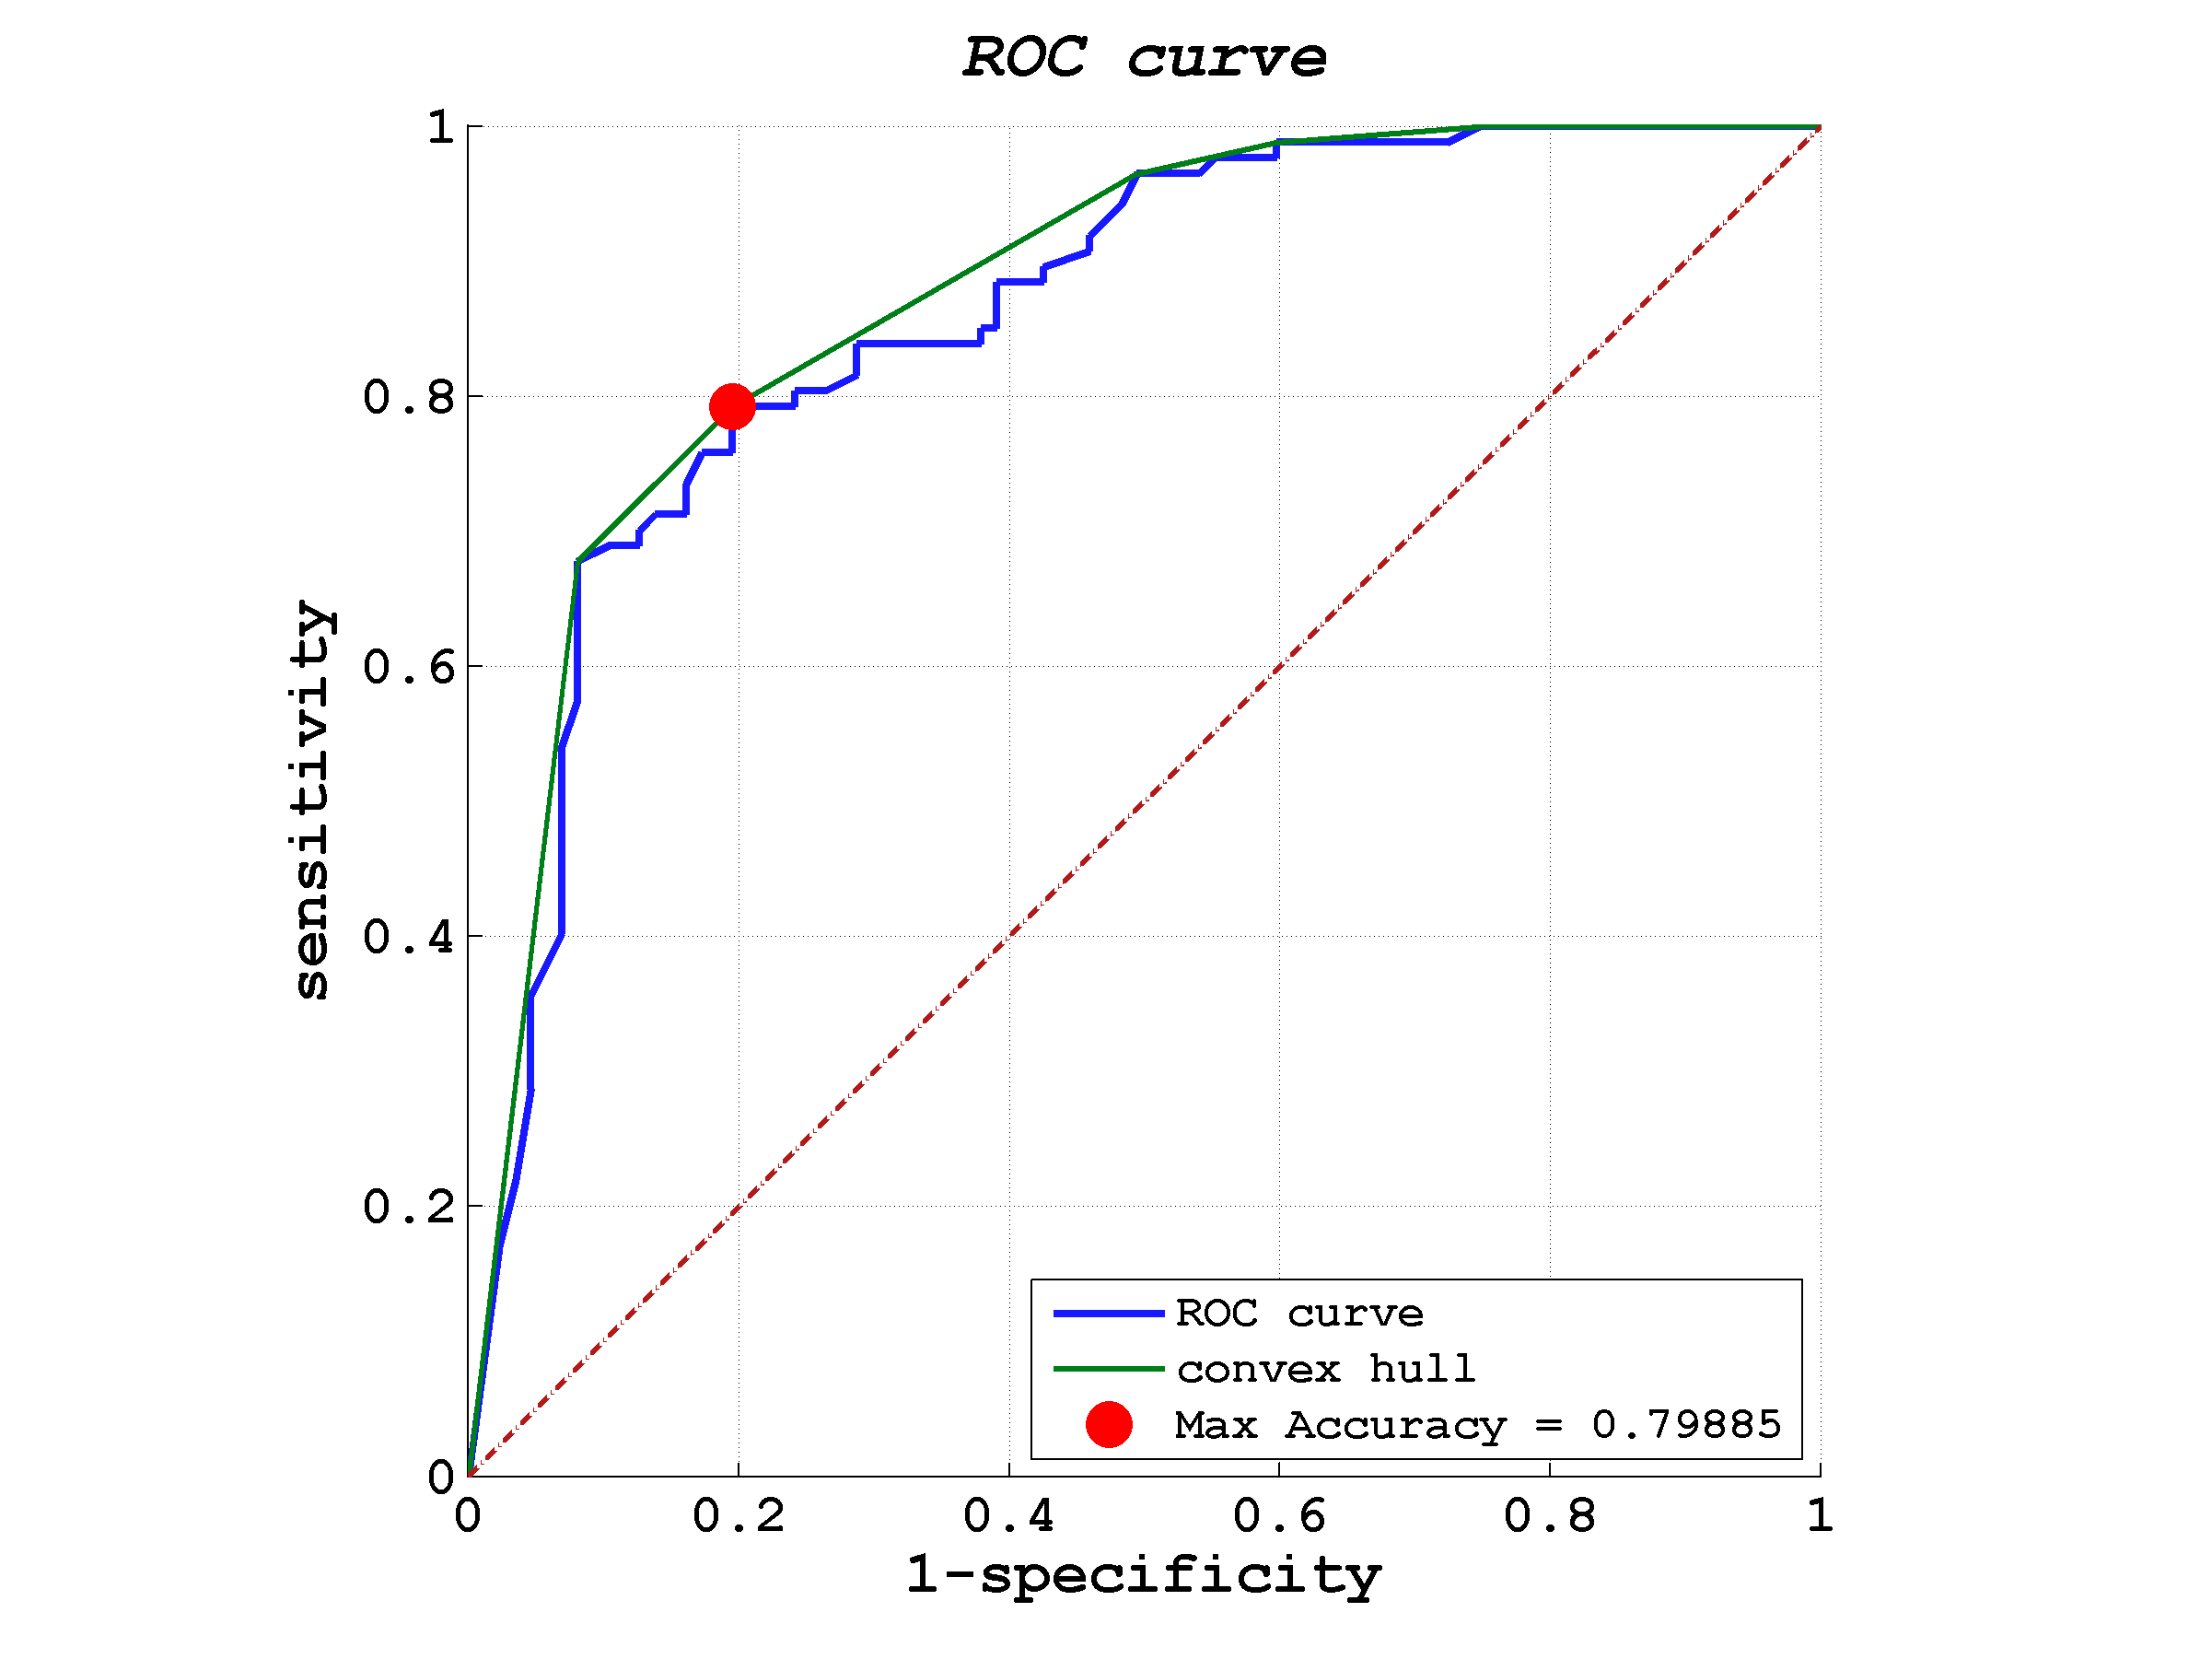
\includegraphics[width=0.46\textwidth]{./images/exp02/SVMprob_MSiHU_def.png}
      \label{ch6:fig3:a}
    }
    \hspace{1mm}
    \subfigure[SVM ext-T - ROC]{
      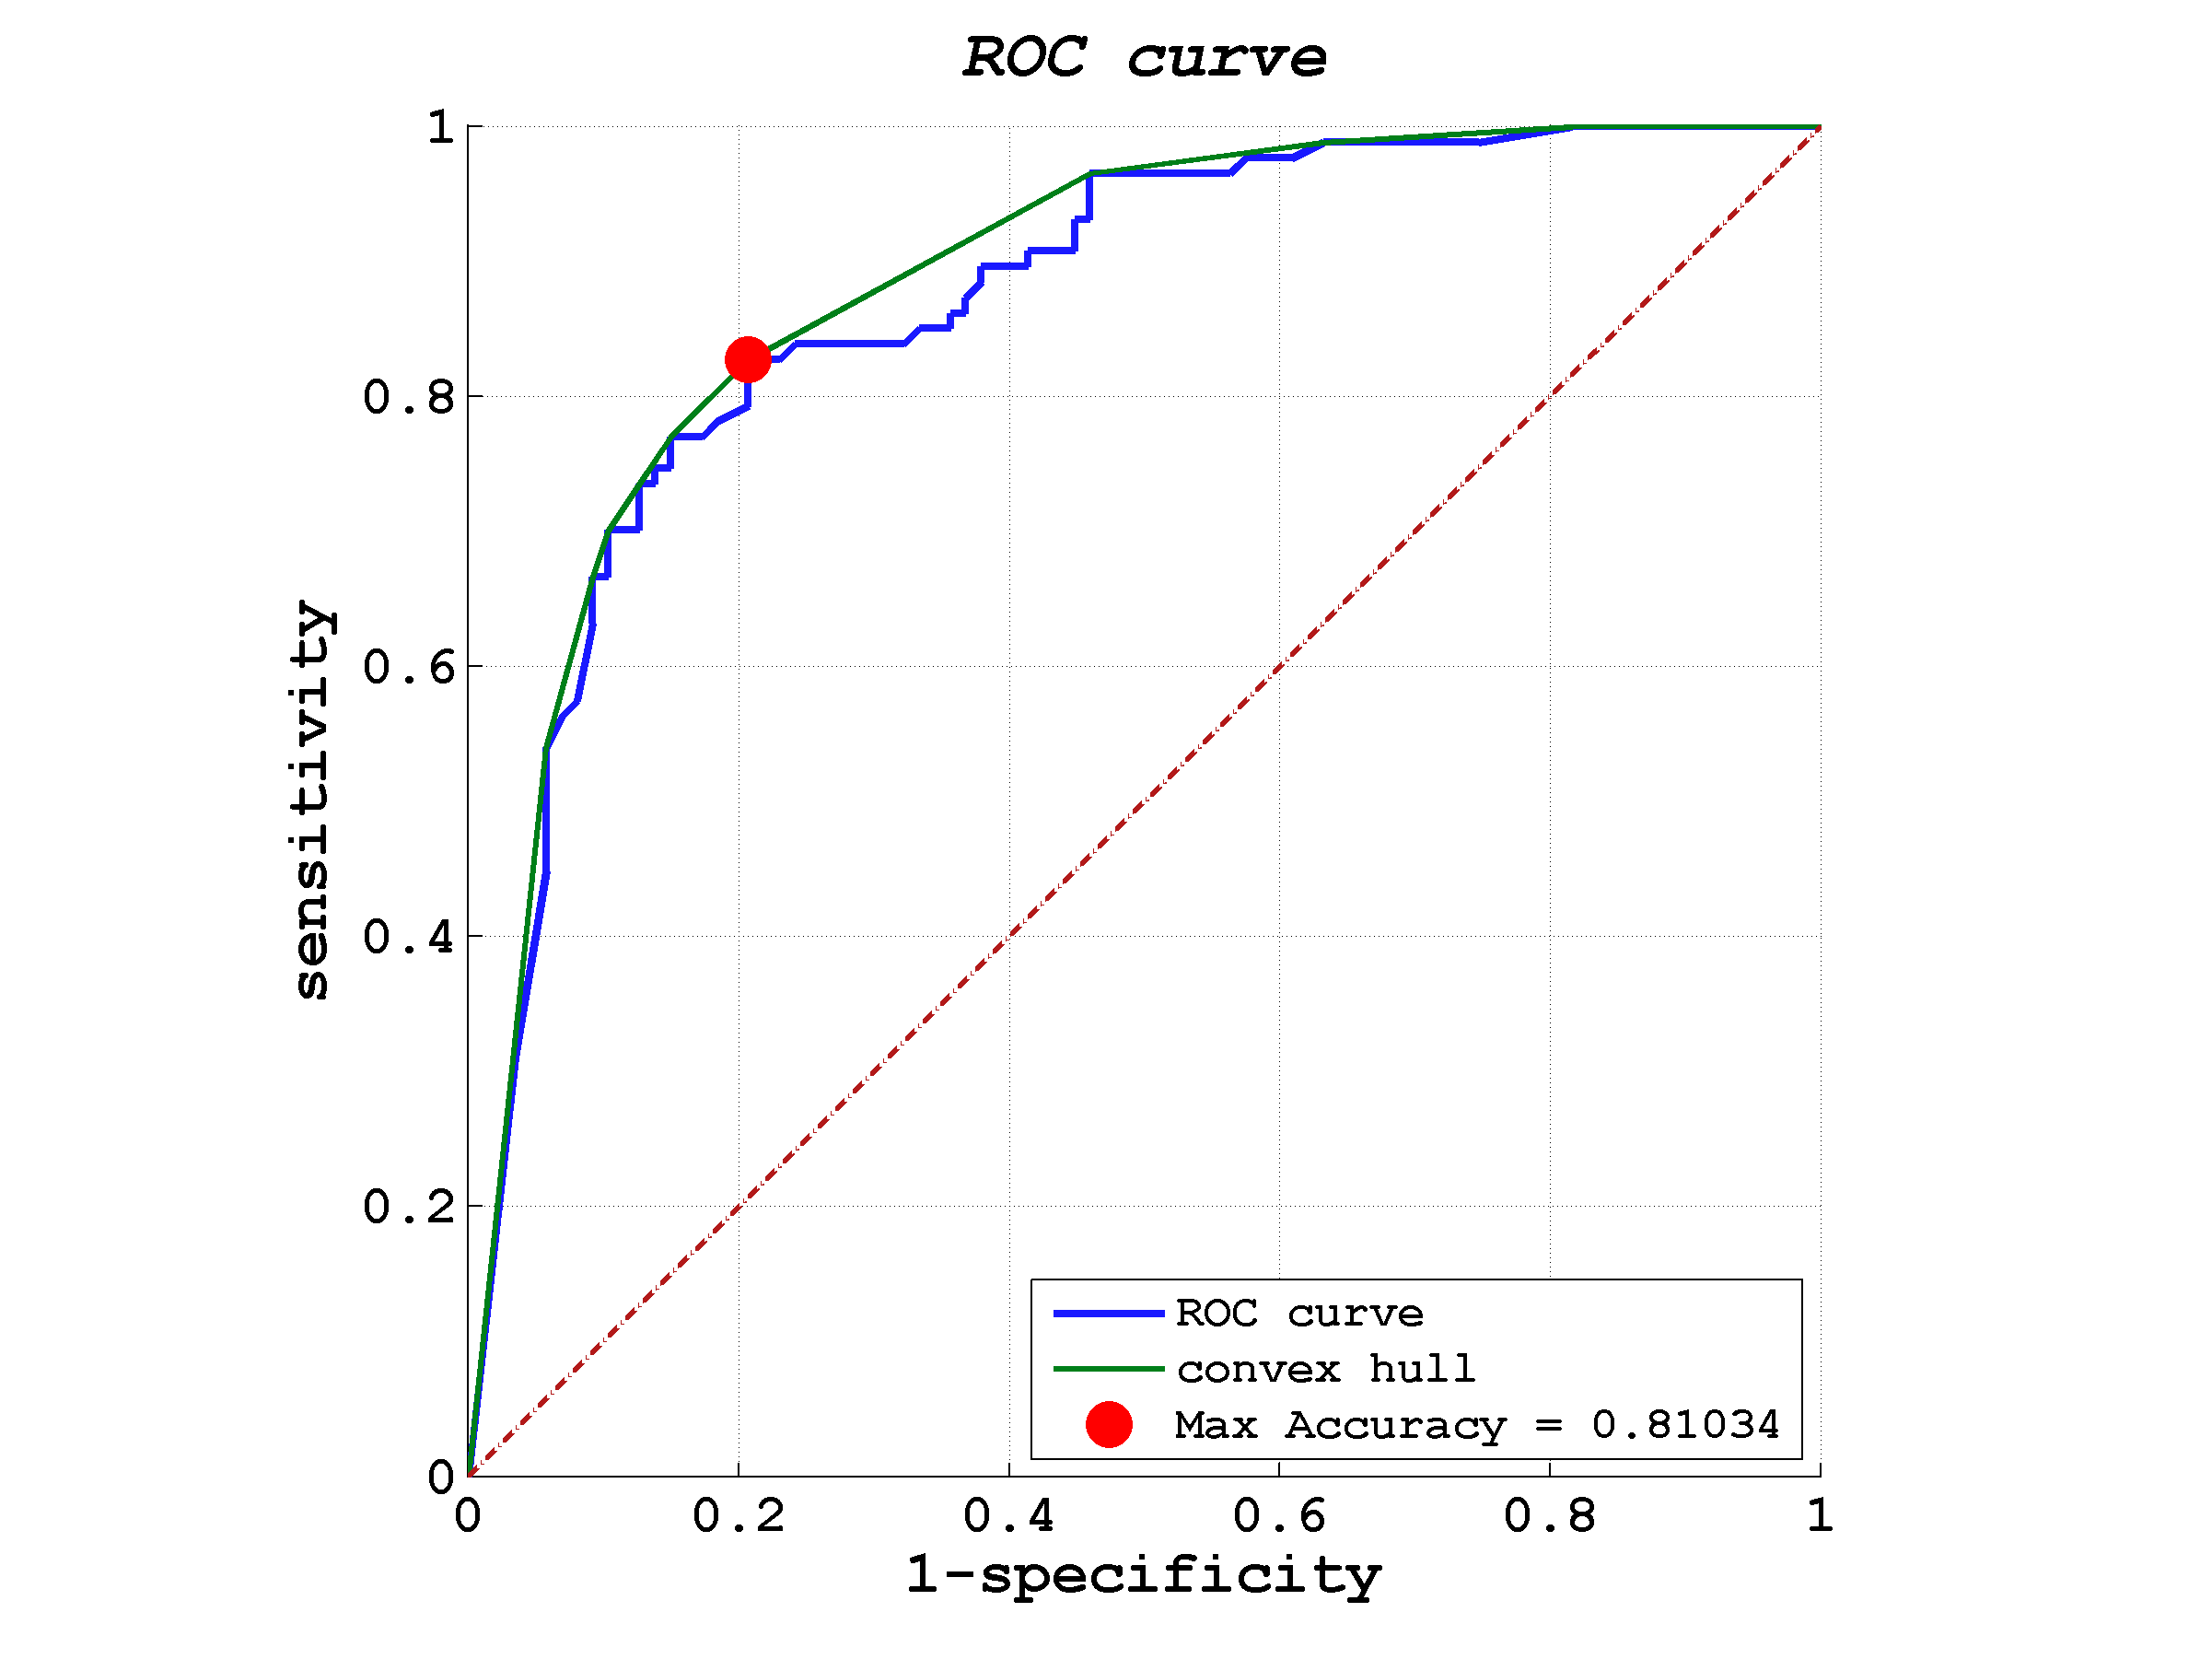
\includegraphics[width=0.46\textwidth]{./images/exp02/SVMprob_MSiHU_extT.png}
      \label{ch6:fig3:b}
    }
    \\
    \subfigure[SVM ext-E - ROC]{
      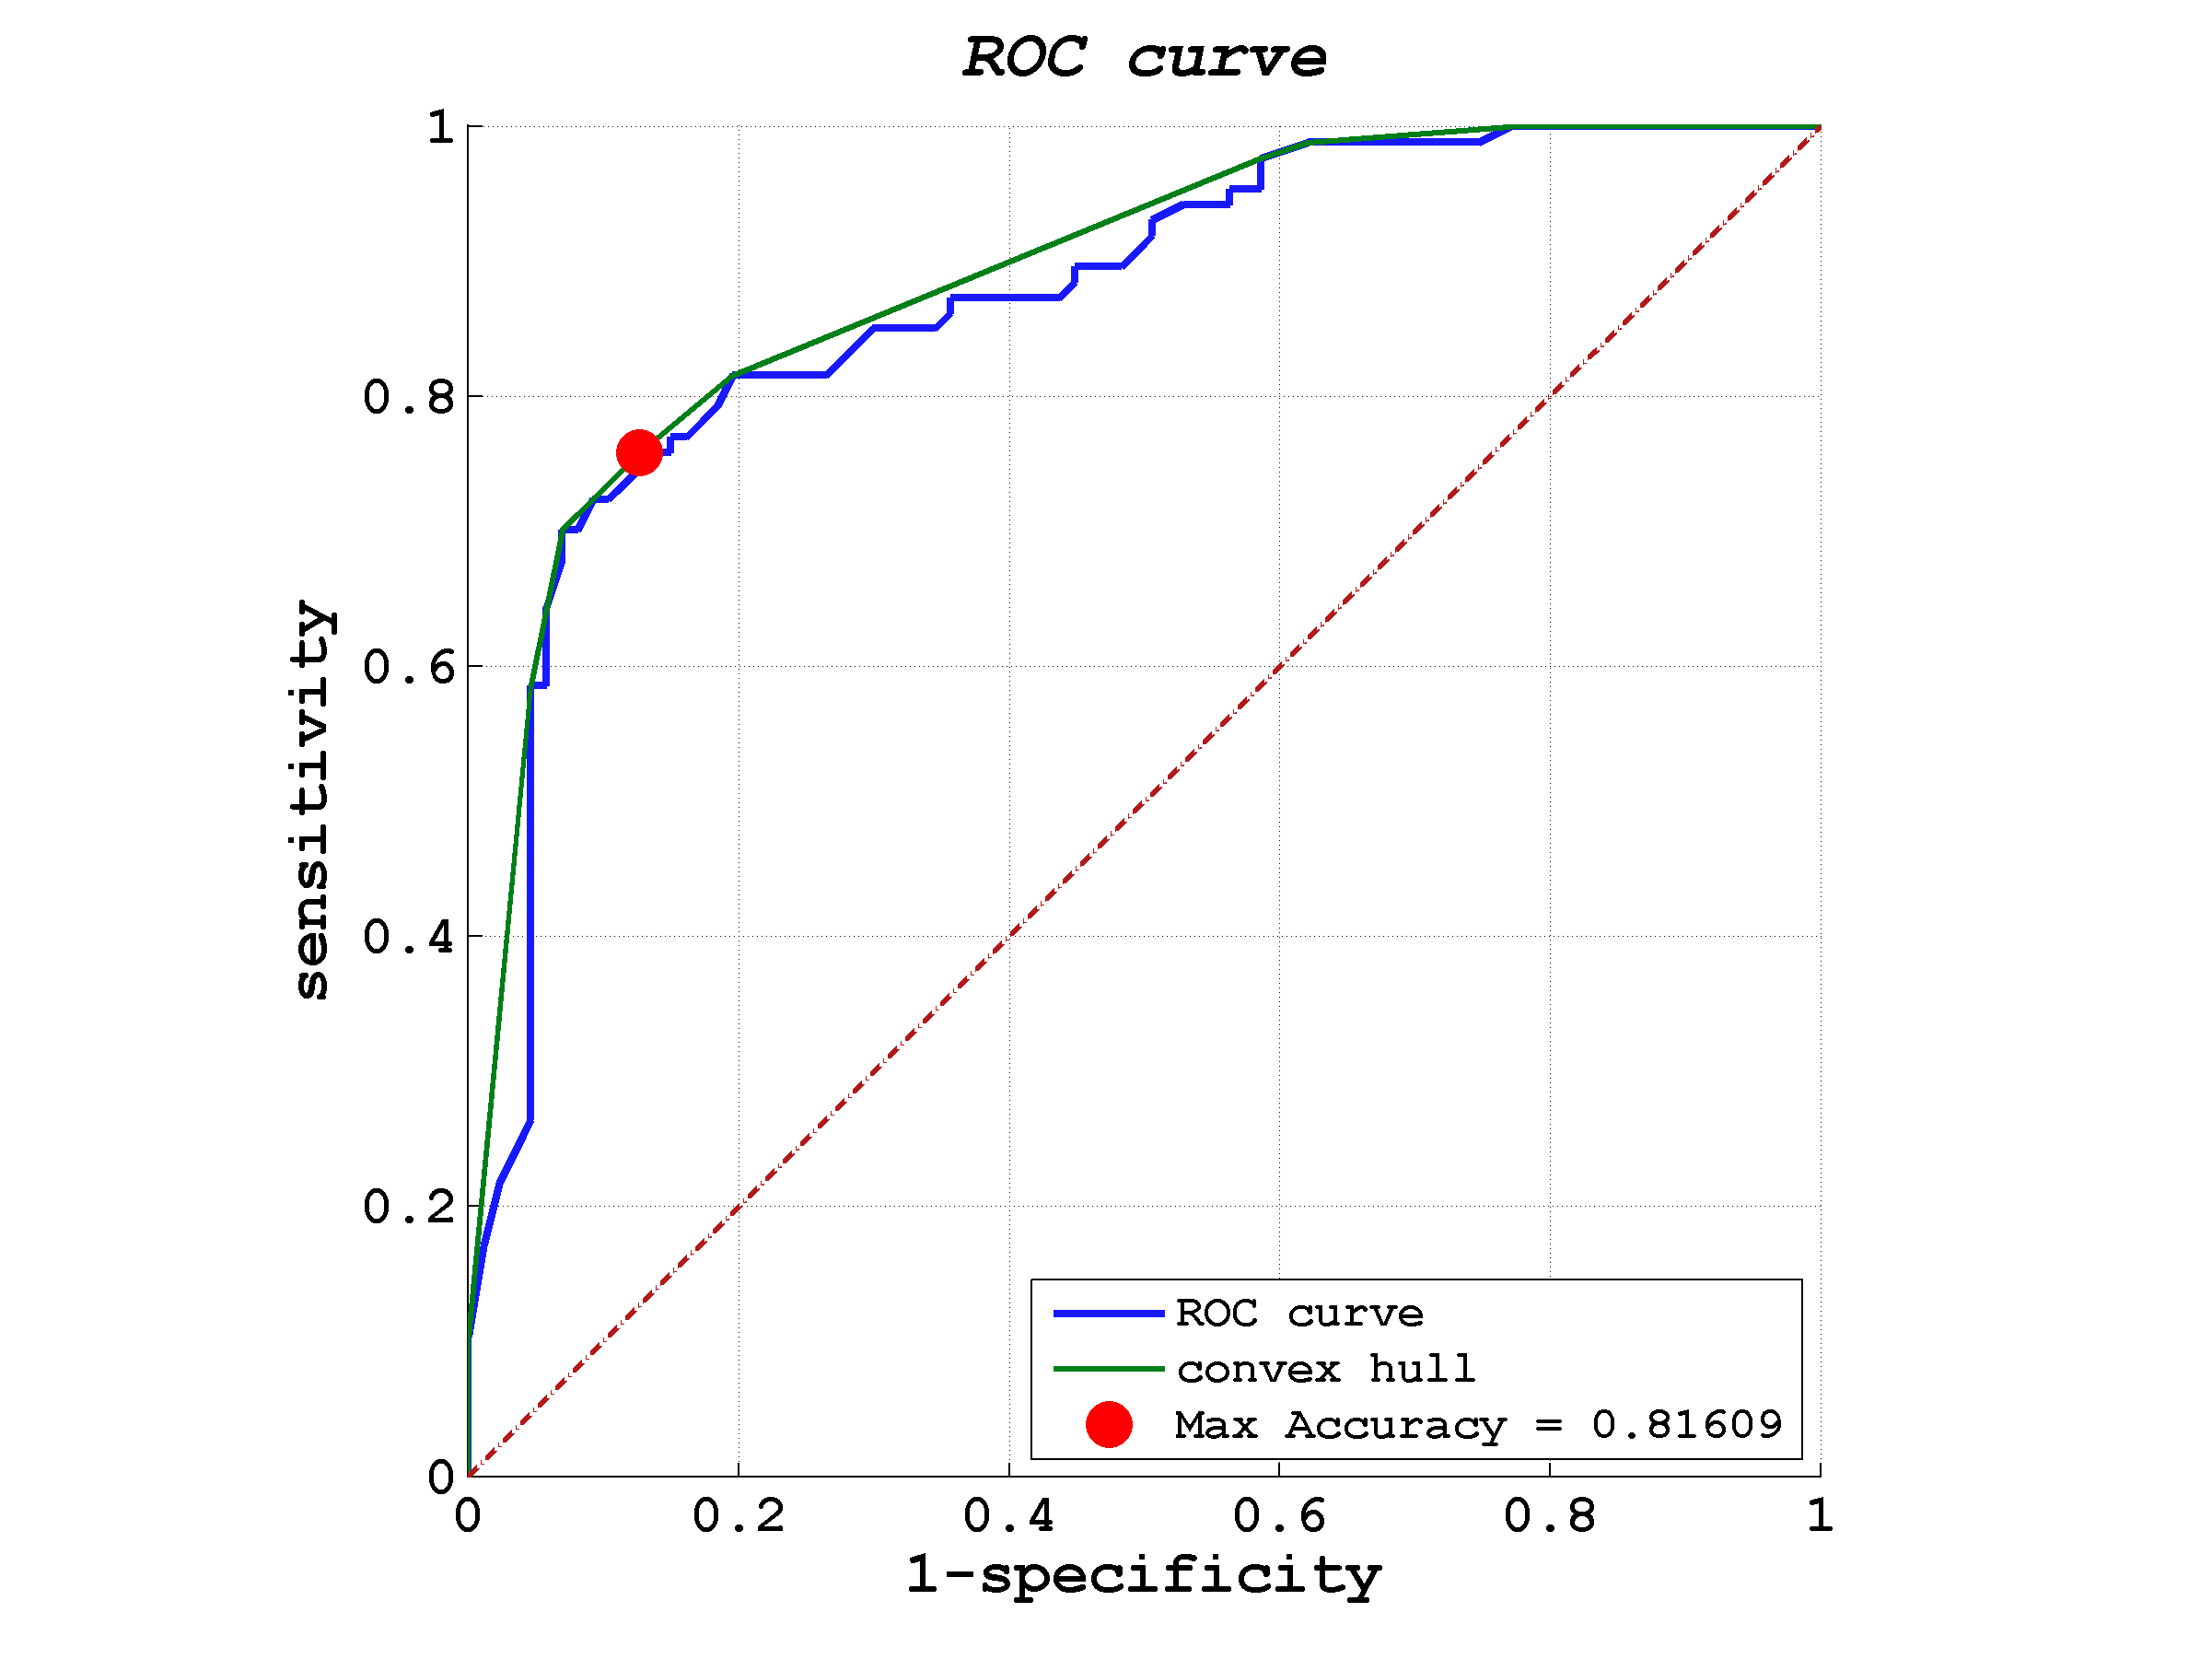
\includegraphics[width=0.46\textwidth]{./images/exp02/SVMprob_MSiHU_extE.png}
      \label{ch6:fig3:c}
    }    
    \hspace{1mm}
    \subfigure[SVM ext-A - ROC]{
      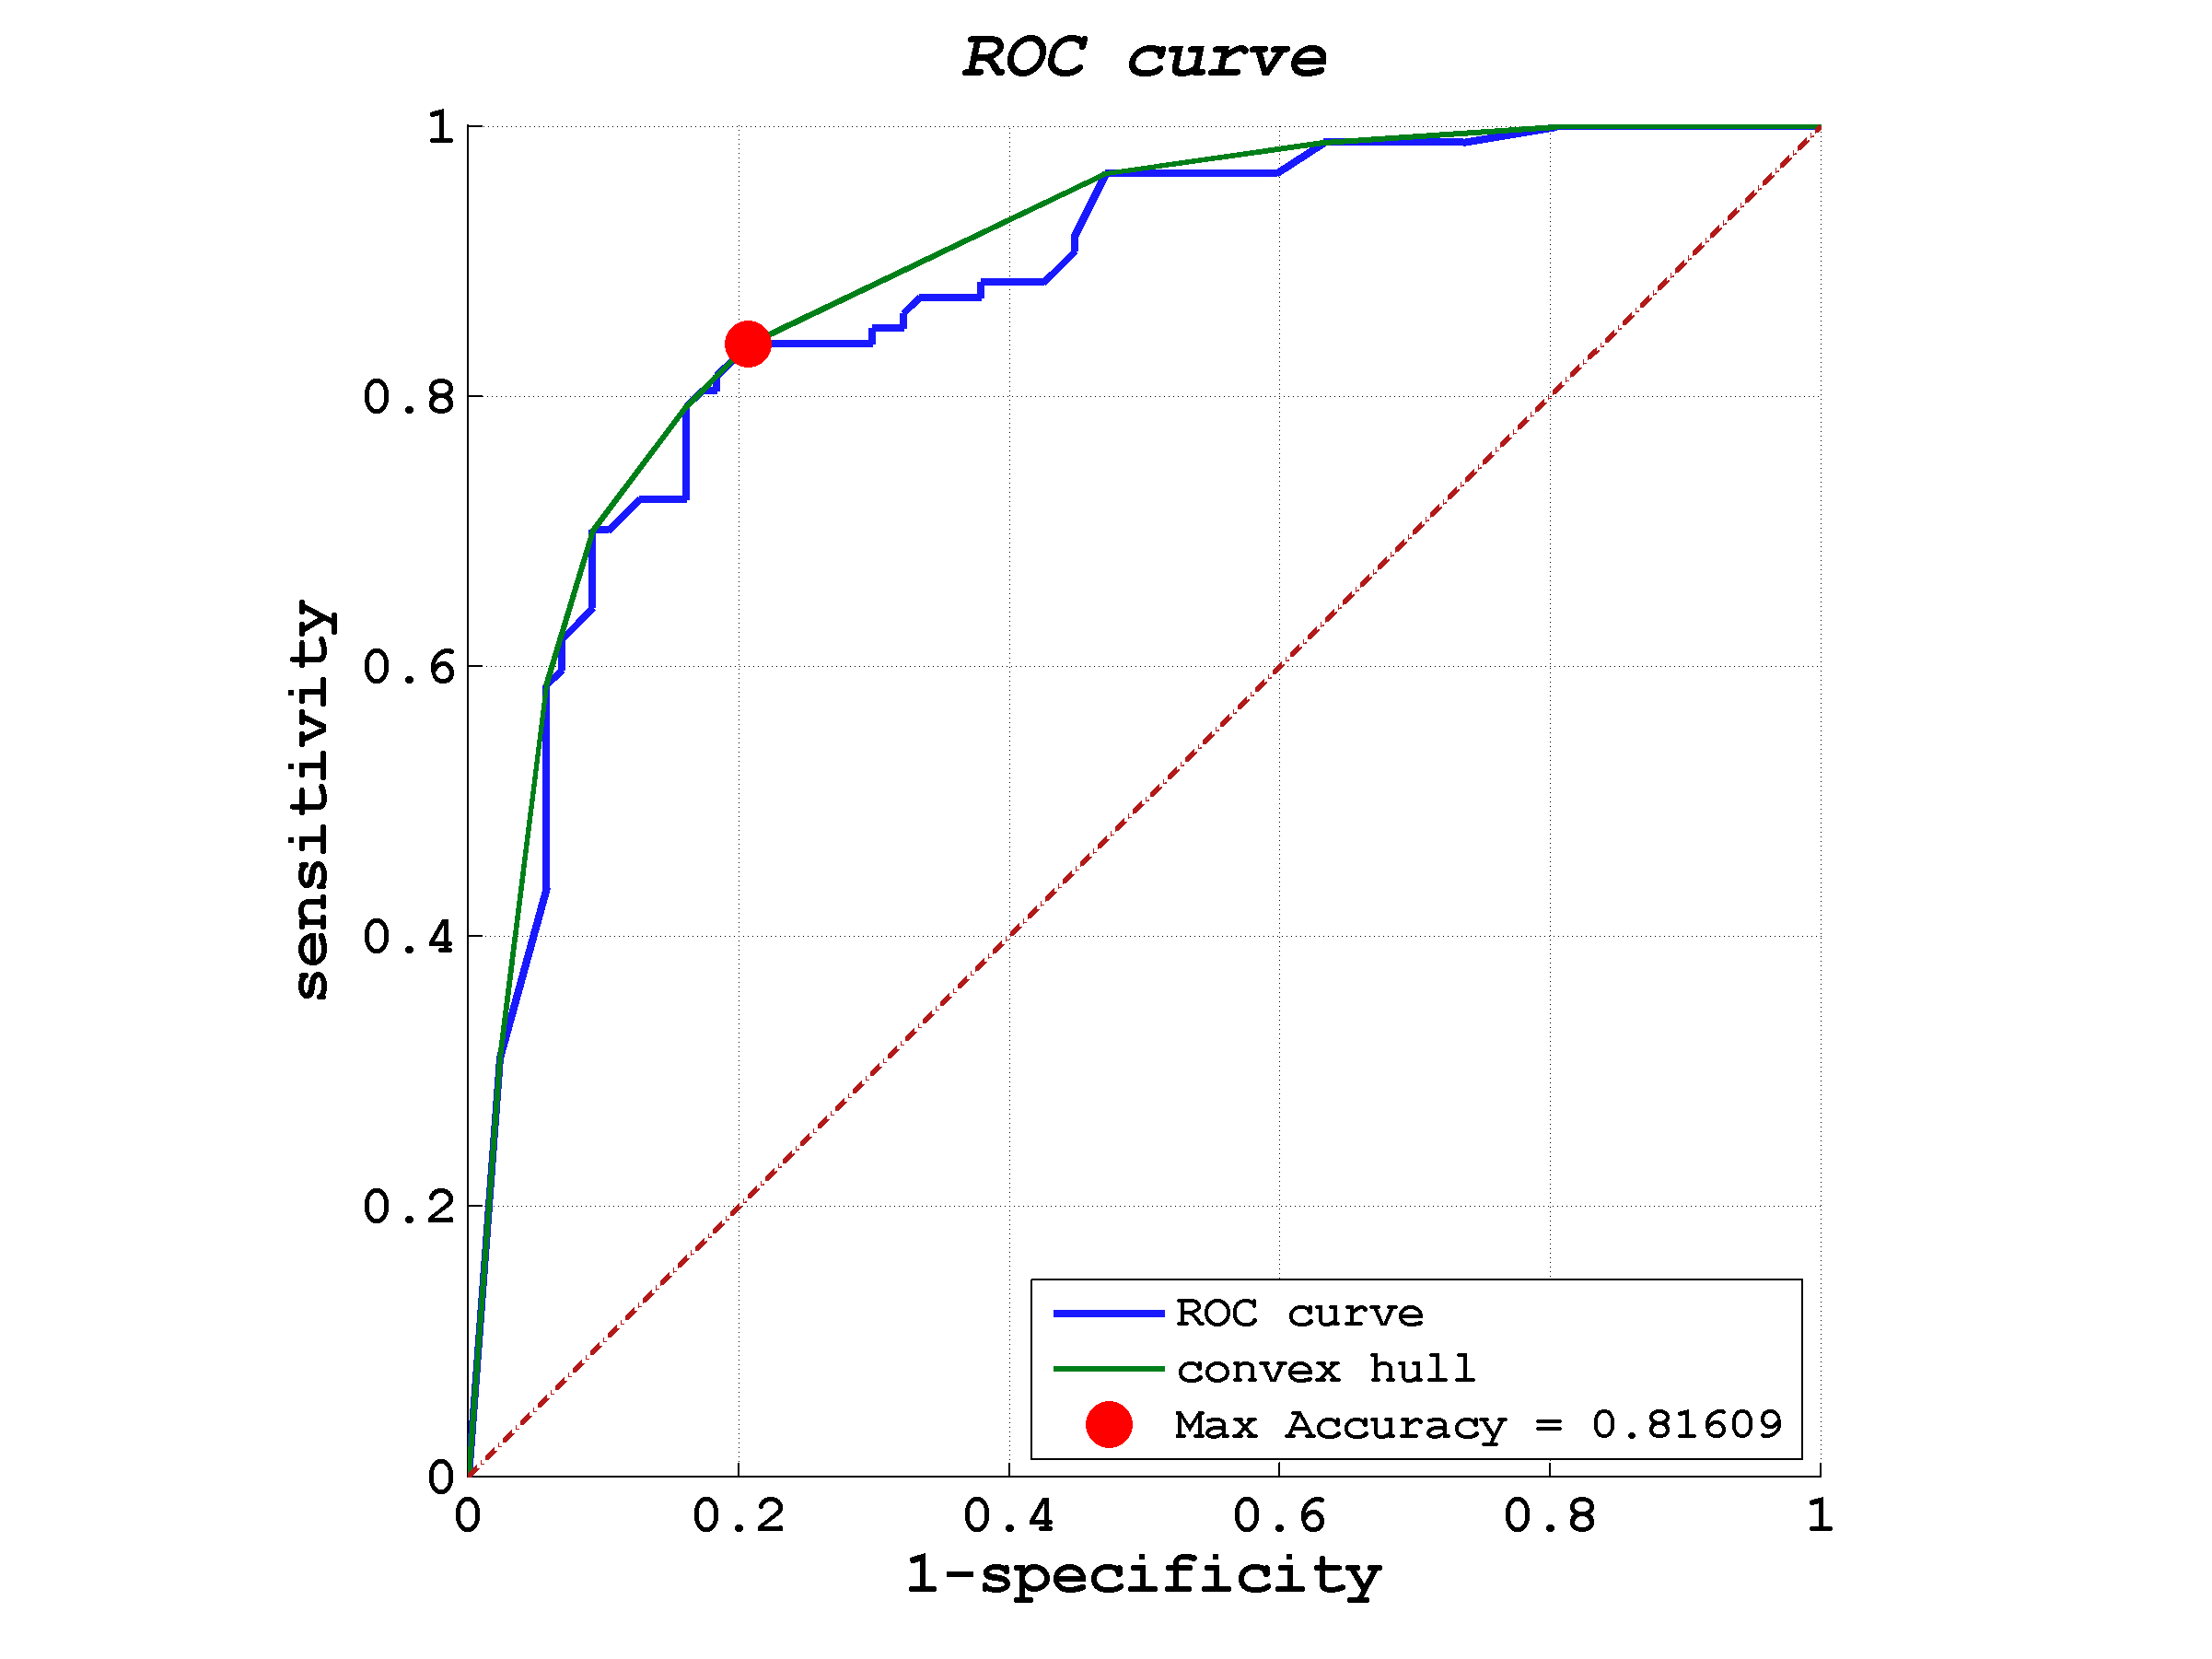
\includegraphics[width=0.46\textwidth]{./images/exp02/SVMprob_MSiHU_extA.png}
      \label{ch6:fig3:d}
    }
    \caption{ROC curves for \texttt{MSiHU} features - SVM classification}
    \label{ch6:fig3}
\end{figure}


\vspace{0.5cm}


\subsubsection{Features: \texttt{MSiHU} - classifier: RF}

We applied our \Gls{RF} classifier to the same dataset, with the results shown in Table \ref{ch6:tab5}.

\begin{table}[!hbt]
\tiny
 \centering
 \begin{tabularx}{350pt}{ >{\centering\arraybackslash} X |>{\centering\arraybackslash} X |>{\centering\arraybackslash} X |>{\centering\arraybackslash} X |>{\centering\arraybackslash} X |>{\centering\arraybackslash} X |>{\centering\arraybackslash} X}
   Classifier     & AUC  & accuracy & precision & F$_1$-Score & sensitivity & specificity \\
   \hline
   \hline
    RF def.      & 0.85 & 78.74\% & 81.25\% & 0.78 & 82.76\% & 74.71\%  \\
    \hline
    RF ext-T     & 0.86 & 79.31\% & 76.29\% & 0.80 & 73.56\% & 85.06\%  \\
    \hline
    RF ext-E     & 0.86 & 78.16\% & 74.75\% & 0.80 & 71.26\% & 85.06\%  \\
    \hline
    RF ext-A     & 0.86 & 77.59\% & 74.00\% & 0.79 & 70.11\% & 85.06\% \\
 \end{tabularx}
 \caption{\texttt{MSiHU} results (RF)}
 \label{ch6:tab5}
\end{table}
 

 
More in detail, the number of classified images at optimal threshold is reported in Table \ref{ch6:tab6}.


\begin{table}[!hbt]
\tiny
 \centering
 \begin{tabularx}{320pt}{ >{\centering\arraybackslash} X |>{\centering\arraybackslash} X |>{\centering\arraybackslash} X |>{\centering\arraybackslash} X |>{\centering\arraybackslash} X }
   Classifier     & TP  & FN & TN & FP  \\
   \hline
   \hline
    RF def.      & 65 & 22 & 72 & 15  \\
    \hline
    RF ext-T     & 74 & 13 & 64 & 23  \\
    \hline
    RF ext-E     & 74 & 13 & 62 & 25  \\
    \hline
    RF ext-A     & 74 & 13 & 61 & 26 \\
 \end{tabularx}
 \caption{\texttt{MSiHU} classified images (RF)}
 \label{ch6:tab6}
\end{table}  

In this classification the extended dataset brings an improvement in the detection of mitoses, while worsens the detection of non-mitoses.
The \Gls{ROC} curves of this classification is shown in Figure \ref{ch6:fig4}.

\begin{figure}[!htb]
  \centering
    \subfigure[RF default - ROC]{
      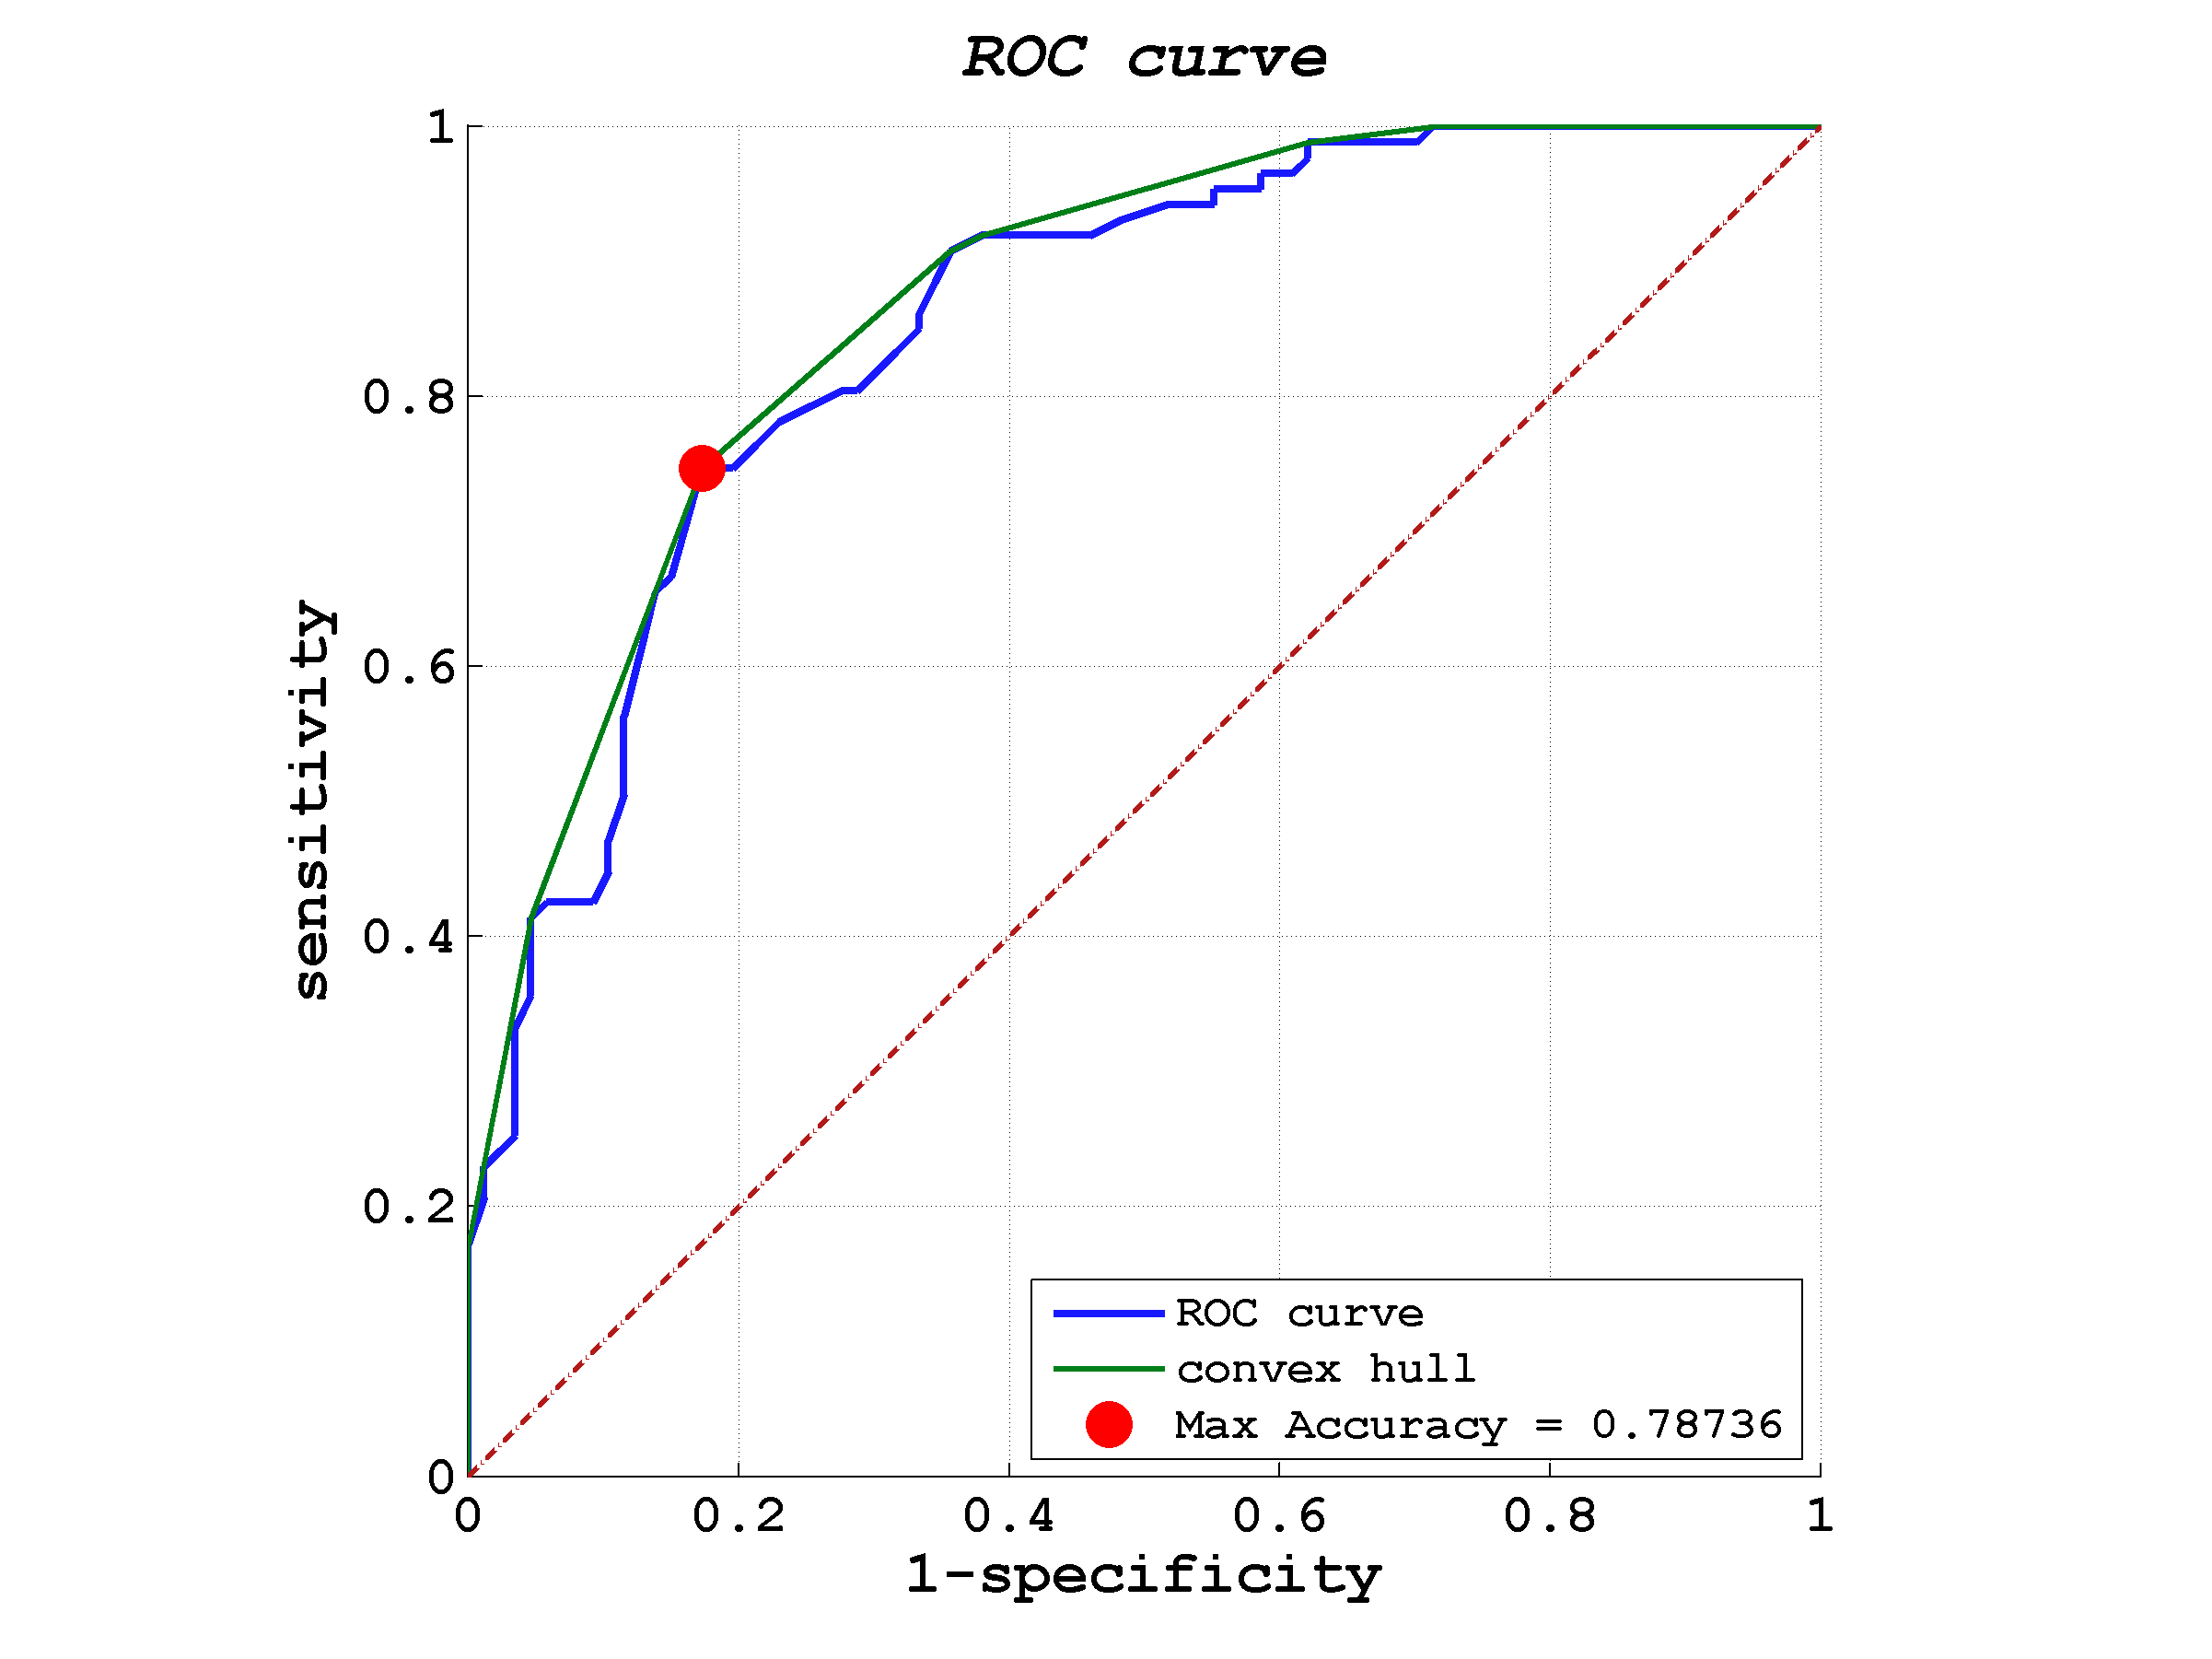
\includegraphics[width=0.46\textwidth]{./images/exp02/RF_MSiHU_def.png}
      \label{ch6:fig4:a}
    }
    \hspace{1mm}
    \subfigure[RF ext-T - ROC]{
      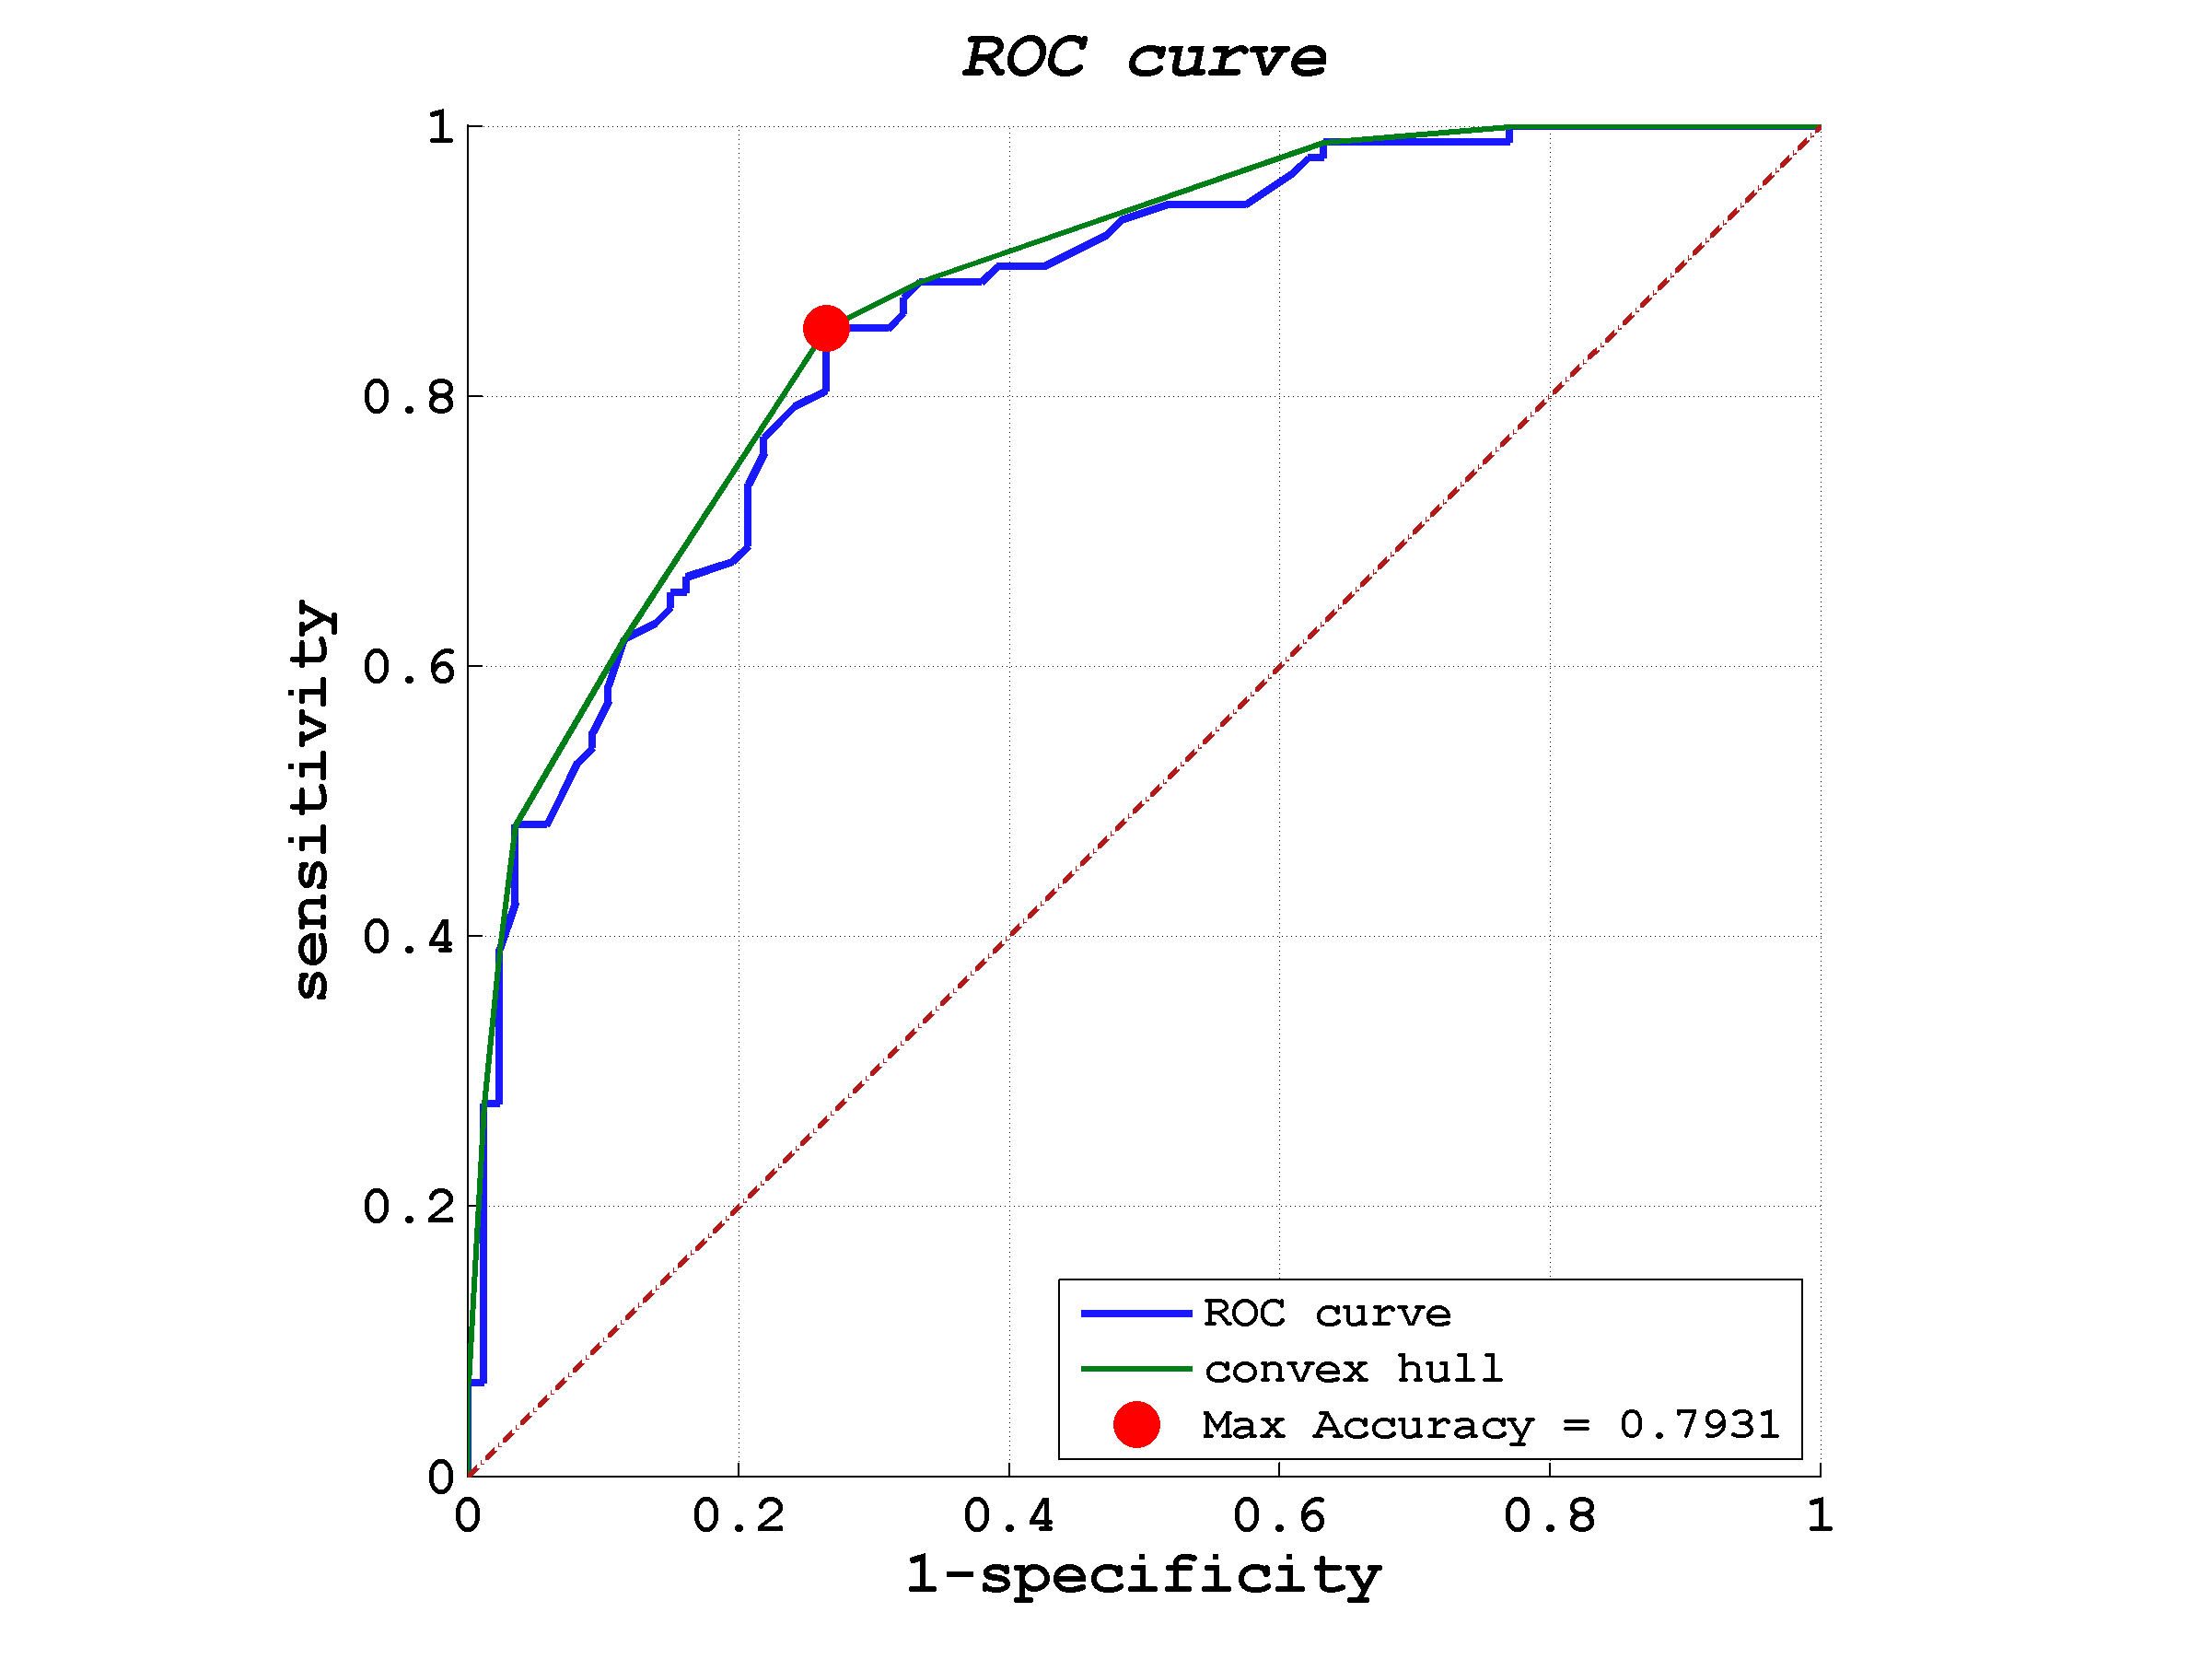
\includegraphics[width=0.46\textwidth]{./images/exp02/RF_MSiHU_extT.png}
      \label{ch6:fig4:b}
    }
    \\
    \subfigure[RF ext-E - ROC]{
      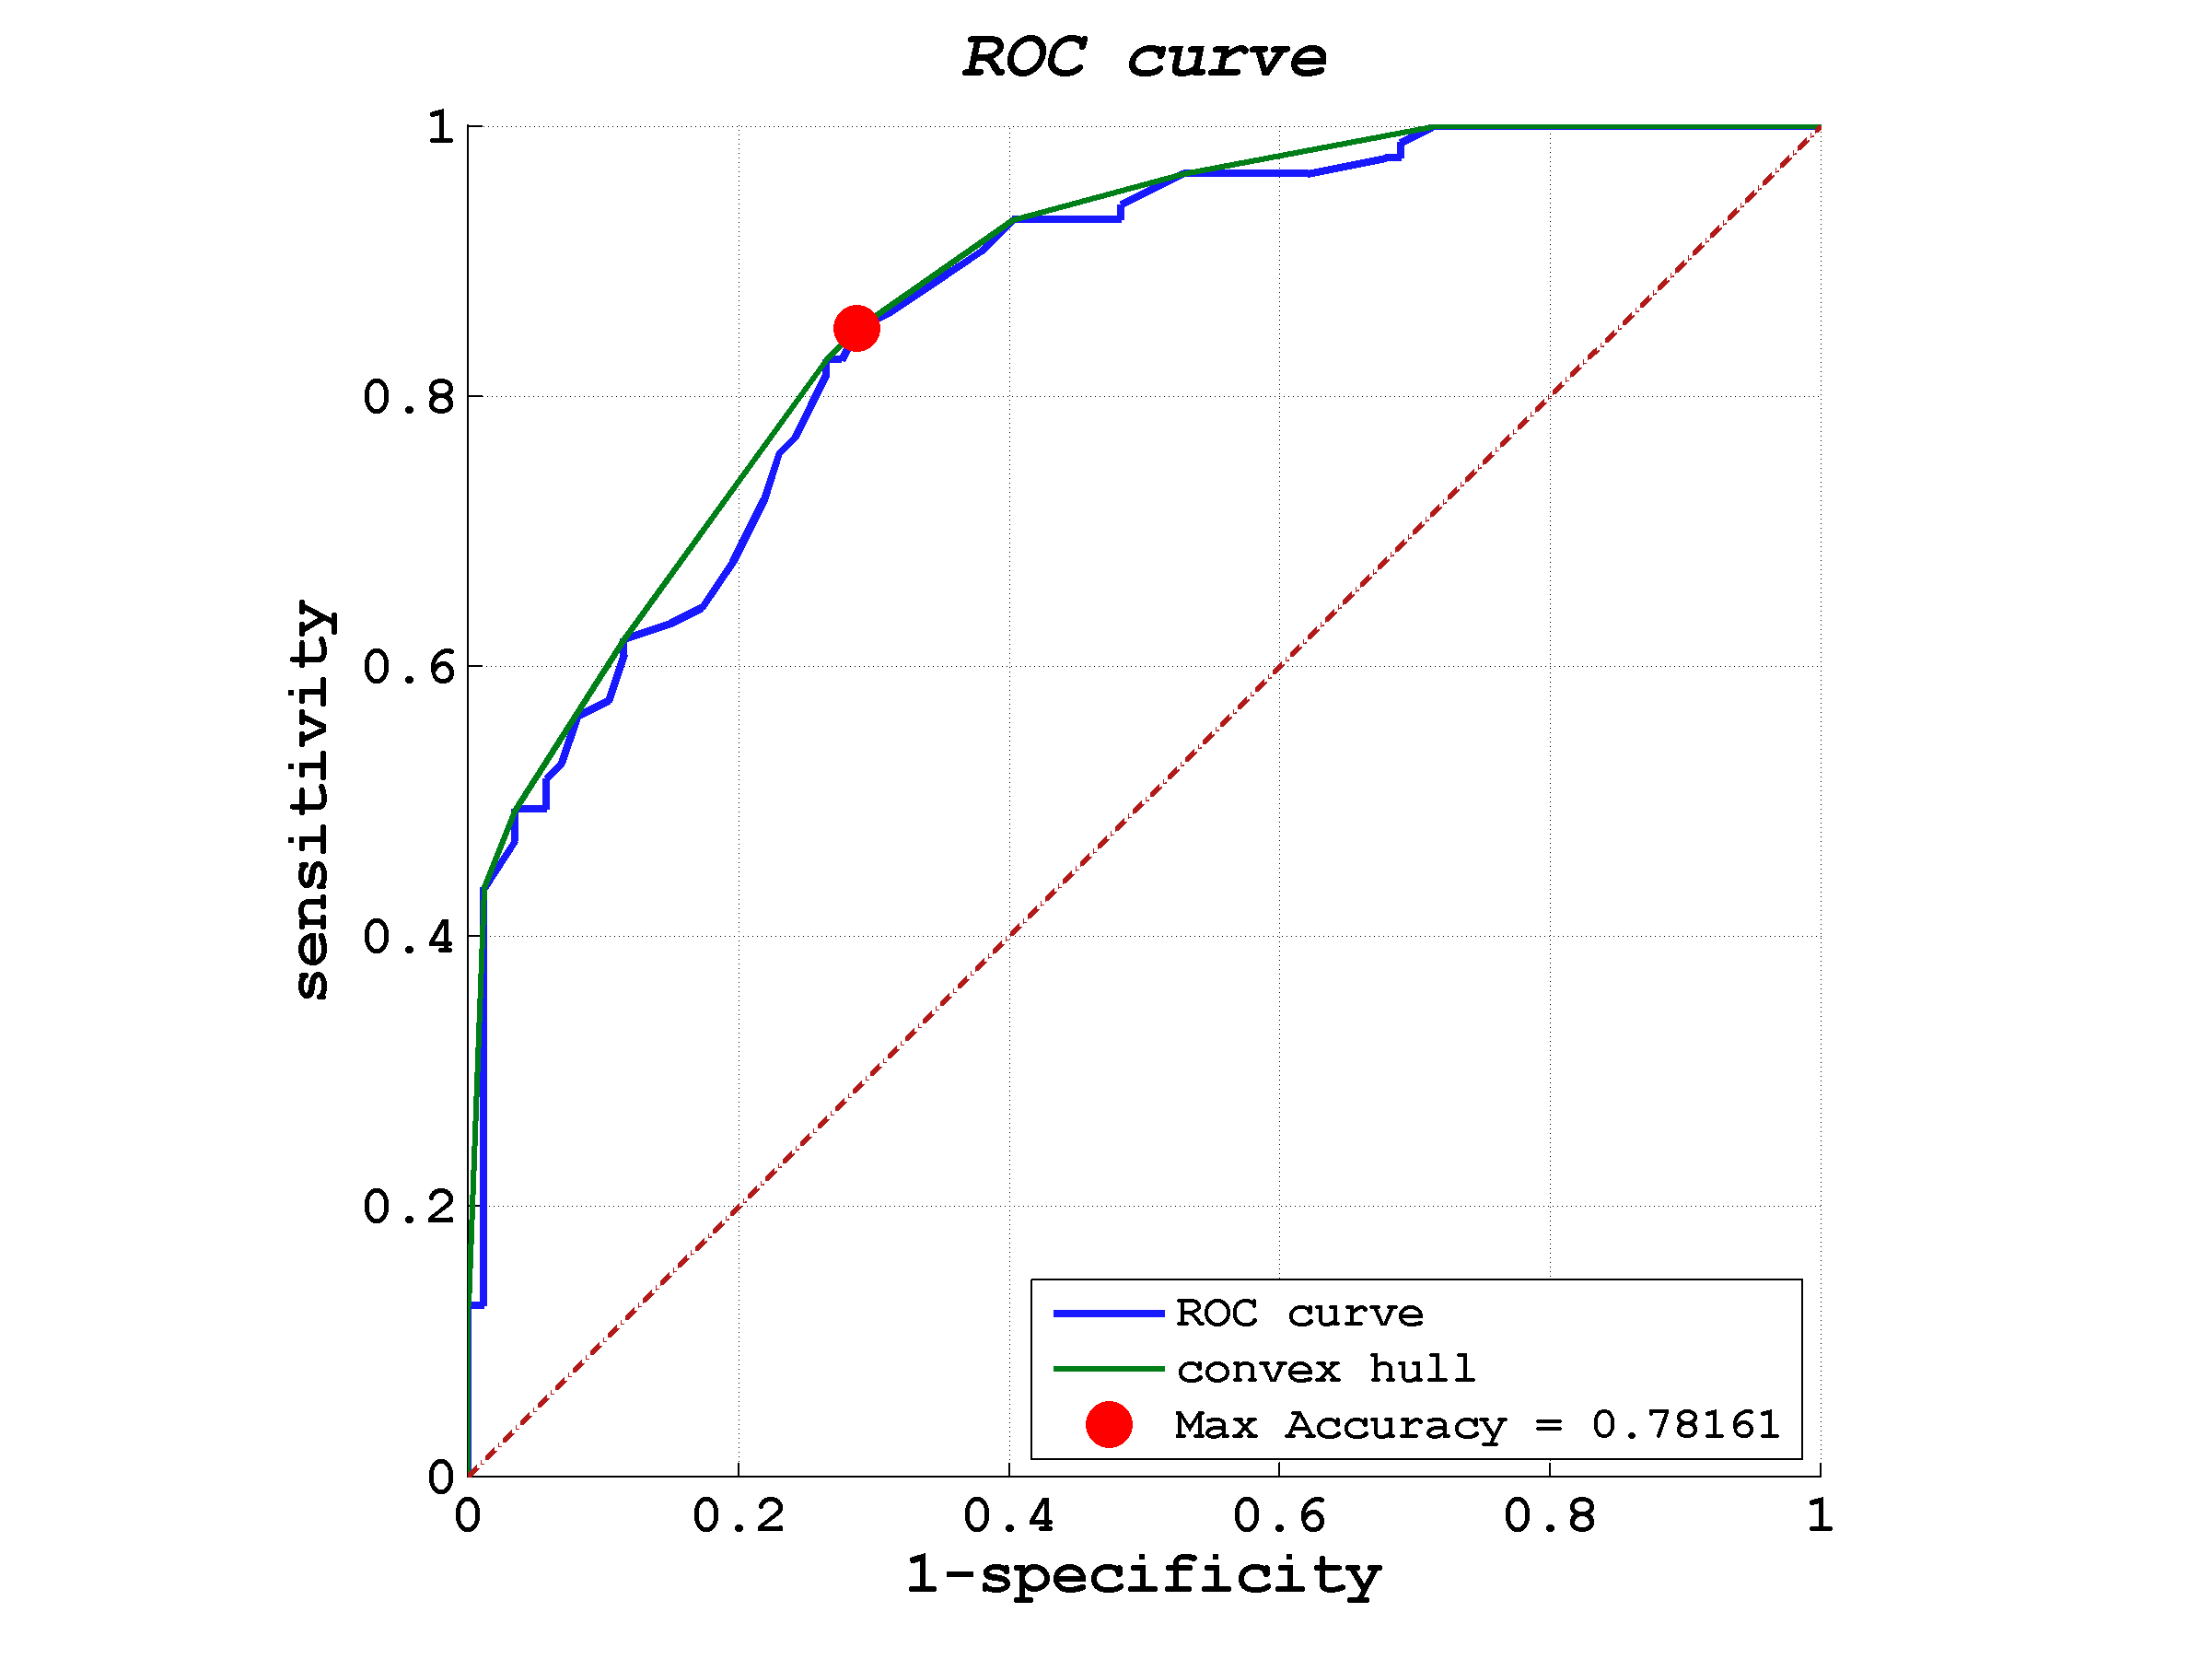
\includegraphics[width=0.46\textwidth]{./images/exp02/RF_MSiHU_extE.png}
      \label{ch6:fig4:c}
    }    
    \hspace{1mm}
    \subfigure[RF ext-A - ROC]{
      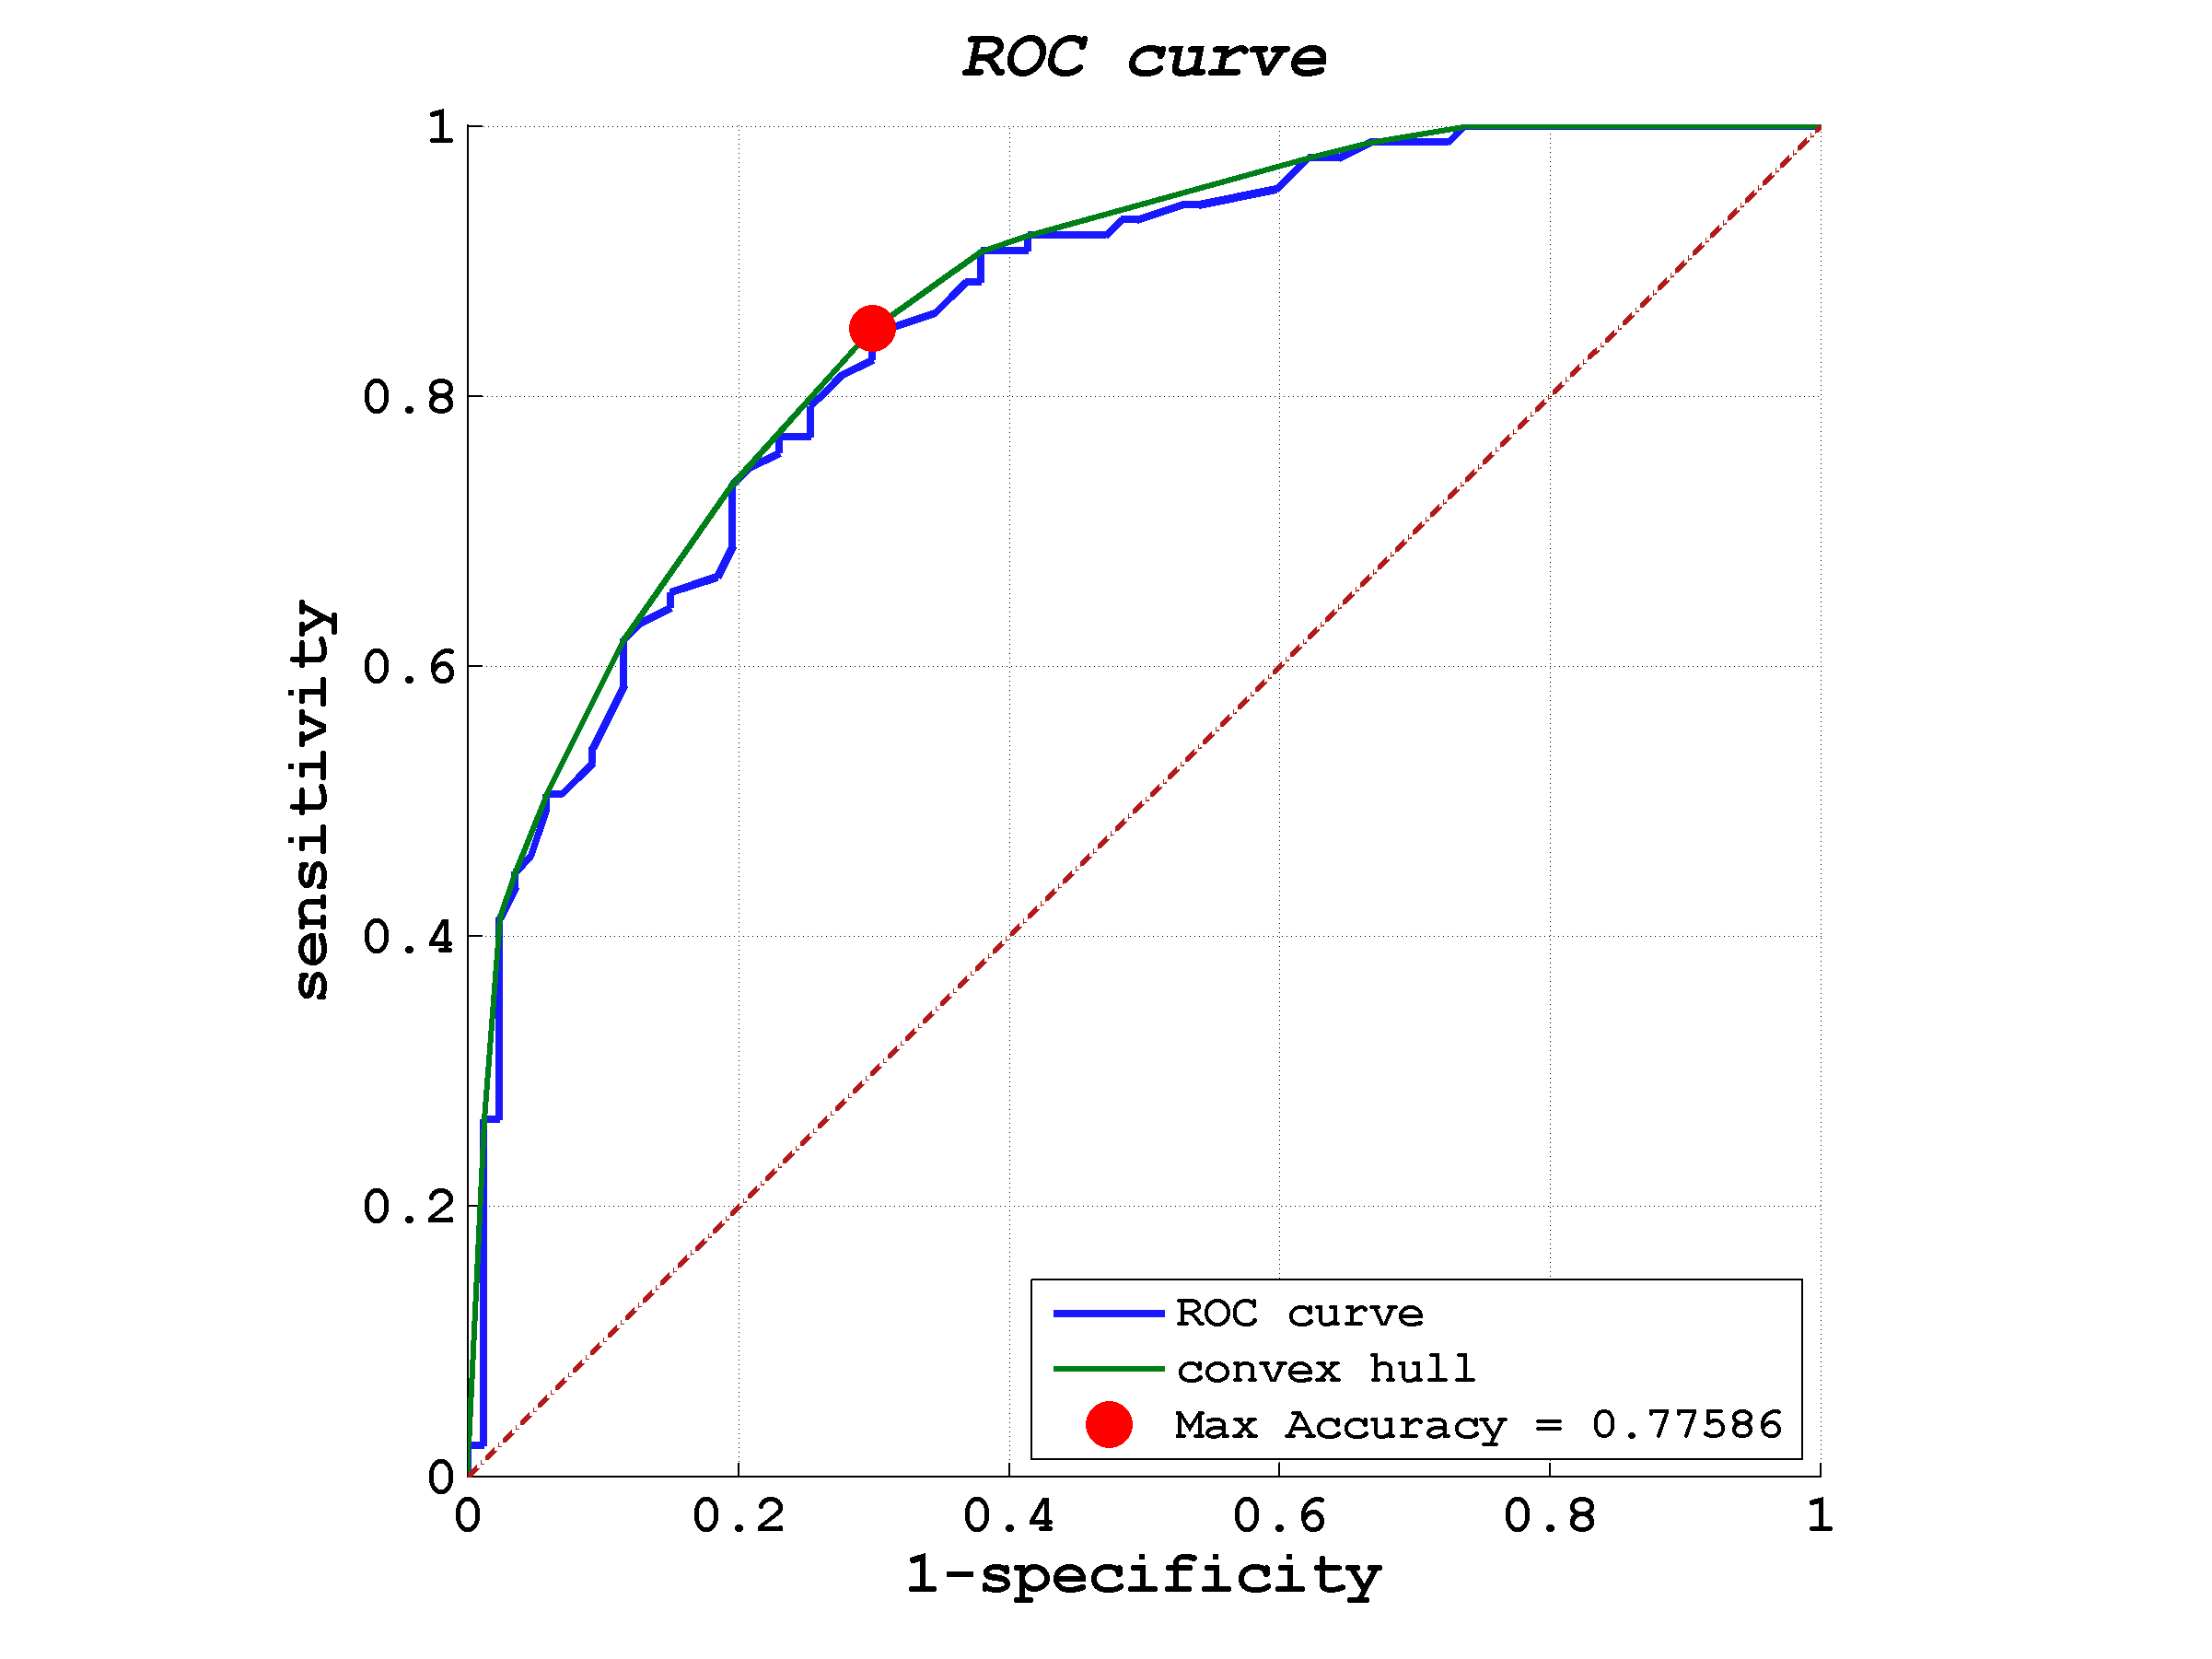
\includegraphics[width=0.46\textwidth]{./images/exp02/RF_MSiHU_extA.png}
      \label{ch6:fig4:d}
    }
    \caption{ROC curves for \texttt{MSiHU} features - RF classification}
    \label{ch6:fig4}
\end{figure}


\vspace{0.5cm}

\subsubsection{Features: \texttt{MSiHR} - classifier: RF}

We applied our \Gls{RF} classifier to the feature-set coded \texttt{MSiHR}, which is an orientation independent dataset. The results are shown in Table \ref{ch6:tab7}.


\begin{table}[!hbt]
\tiny
 \centering
 \begin{tabularx}{350pt}{ >{\centering\arraybackslash} X |>{\centering\arraybackslash} X |>{\centering\arraybackslash} X |>{\centering\arraybackslash} X |>{\centering\arraybackslash} X |>{\centering\arraybackslash} X |>{\centering\arraybackslash} X}
   Classifier     & AUC  & accuracy & precision & F$_1$-Score & sensitivity & specificity \\
   \hline
   \hline
    RF def.      & 0.89 & 82.18\% & 84.15\% & 0.82 & 85.06\% & 79.31\%  \\
    \hline
    RF ext-T     & 0.90 & 81.61\% & 83.95\% & 0.81 & 85.06\% & 78.16\%  \\
    \hline
    RF ext-E     & 0.89 & 81.61\% & 85.71\% & 0.80 & 87.36\% & 75.86\%  \\
    \hline
    RF ext-A     & 0.90 & 81.03\% & 85.53\% & 0.80 & 87.36\% & 74.71\% \\
 \end{tabularx}
 \caption{\texttt{MSiHR} results (RF)}
 \label{ch6:tab7}
\end{table}
  
  
More in detail, the number of classified images at optimal threshold is reported in Table \ref{ch6:tab8}.


\begin{table}[!hbt]
\tiny
 \centering
 \begin{tabularx}{320pt}{ >{\centering\arraybackslash} X |>{\centering\arraybackslash} X |>{\centering\arraybackslash} X |>{\centering\arraybackslash} X |>{\centering\arraybackslash} X }
   Classifier     & TP  & FN & TN & FP  \\
   \hline
   \hline
    RF def.      & 69 & 18 & 74 & 13  \\
    \hline
    RF ext-T     & 68 & 19 & 74 & 13  \\
    \hline
    RF ext-E     & 66 & 21 & 76 & 11  \\
    \hline
    RF ext-A     & 65 & 22 & 76 & 11 \\
 \end{tabularx}
 \caption{\texttt{MSiHR} classified images (RF)}
 \label{ch6:tab8}
\end{table}  

Looking at Table \ref{ch6:tab8}, the most interesting trend concerns the number of \Glspl{TP}. In fact, using an extended dataset with no rotation dependent features
brings no advantages, instead reduces the number of detected mitoses. In a sense, there is more noise than useful information. On the other hand, it is always visible 
the fact that \Glspl{TN} are better detected with extended datasets.\\
The \Gls{ROC} curves of this classification is shown in Figure \ref{ch6:fig5}.

\begin{figure}[!htb]
  \centering
    \subfigure[RF default - ROC]{
      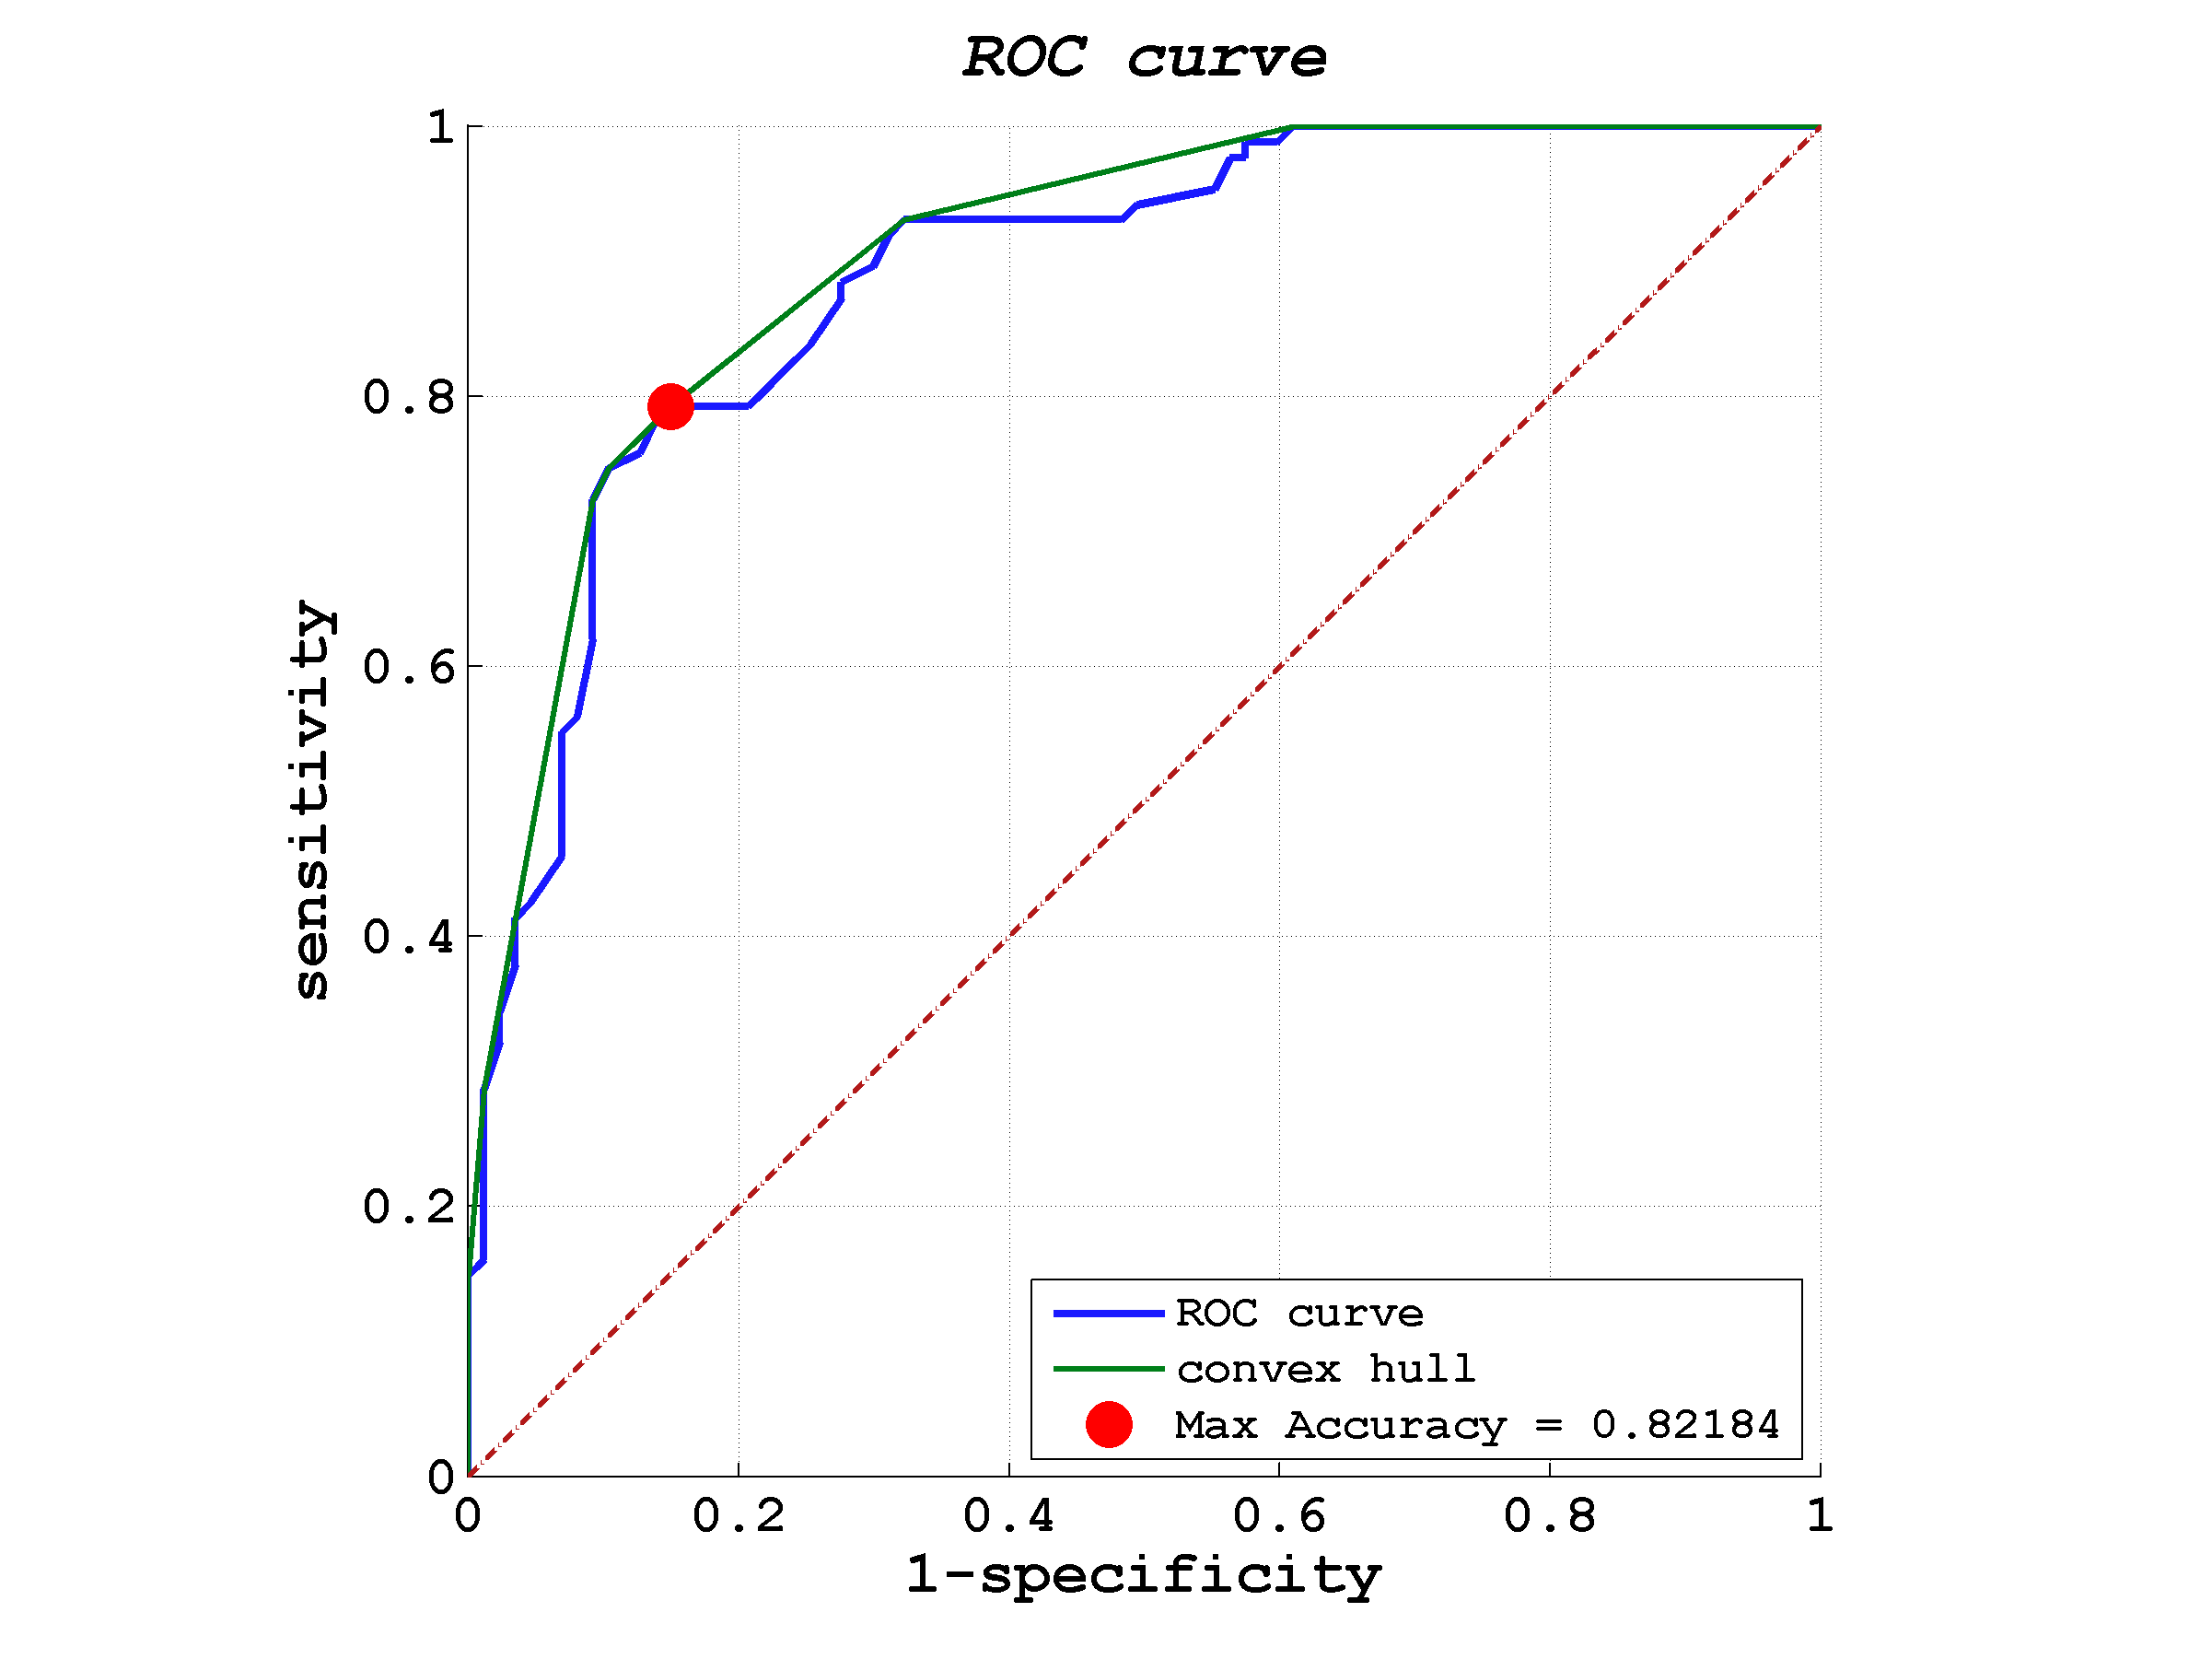
\includegraphics[width=0.46\textwidth]{./images/exp02/RF_MSiHR_def.png}
      \label{ch6:fig5:a}
    }
    \hspace{1mm}
    \subfigure[RF ext-T - ROC]{
      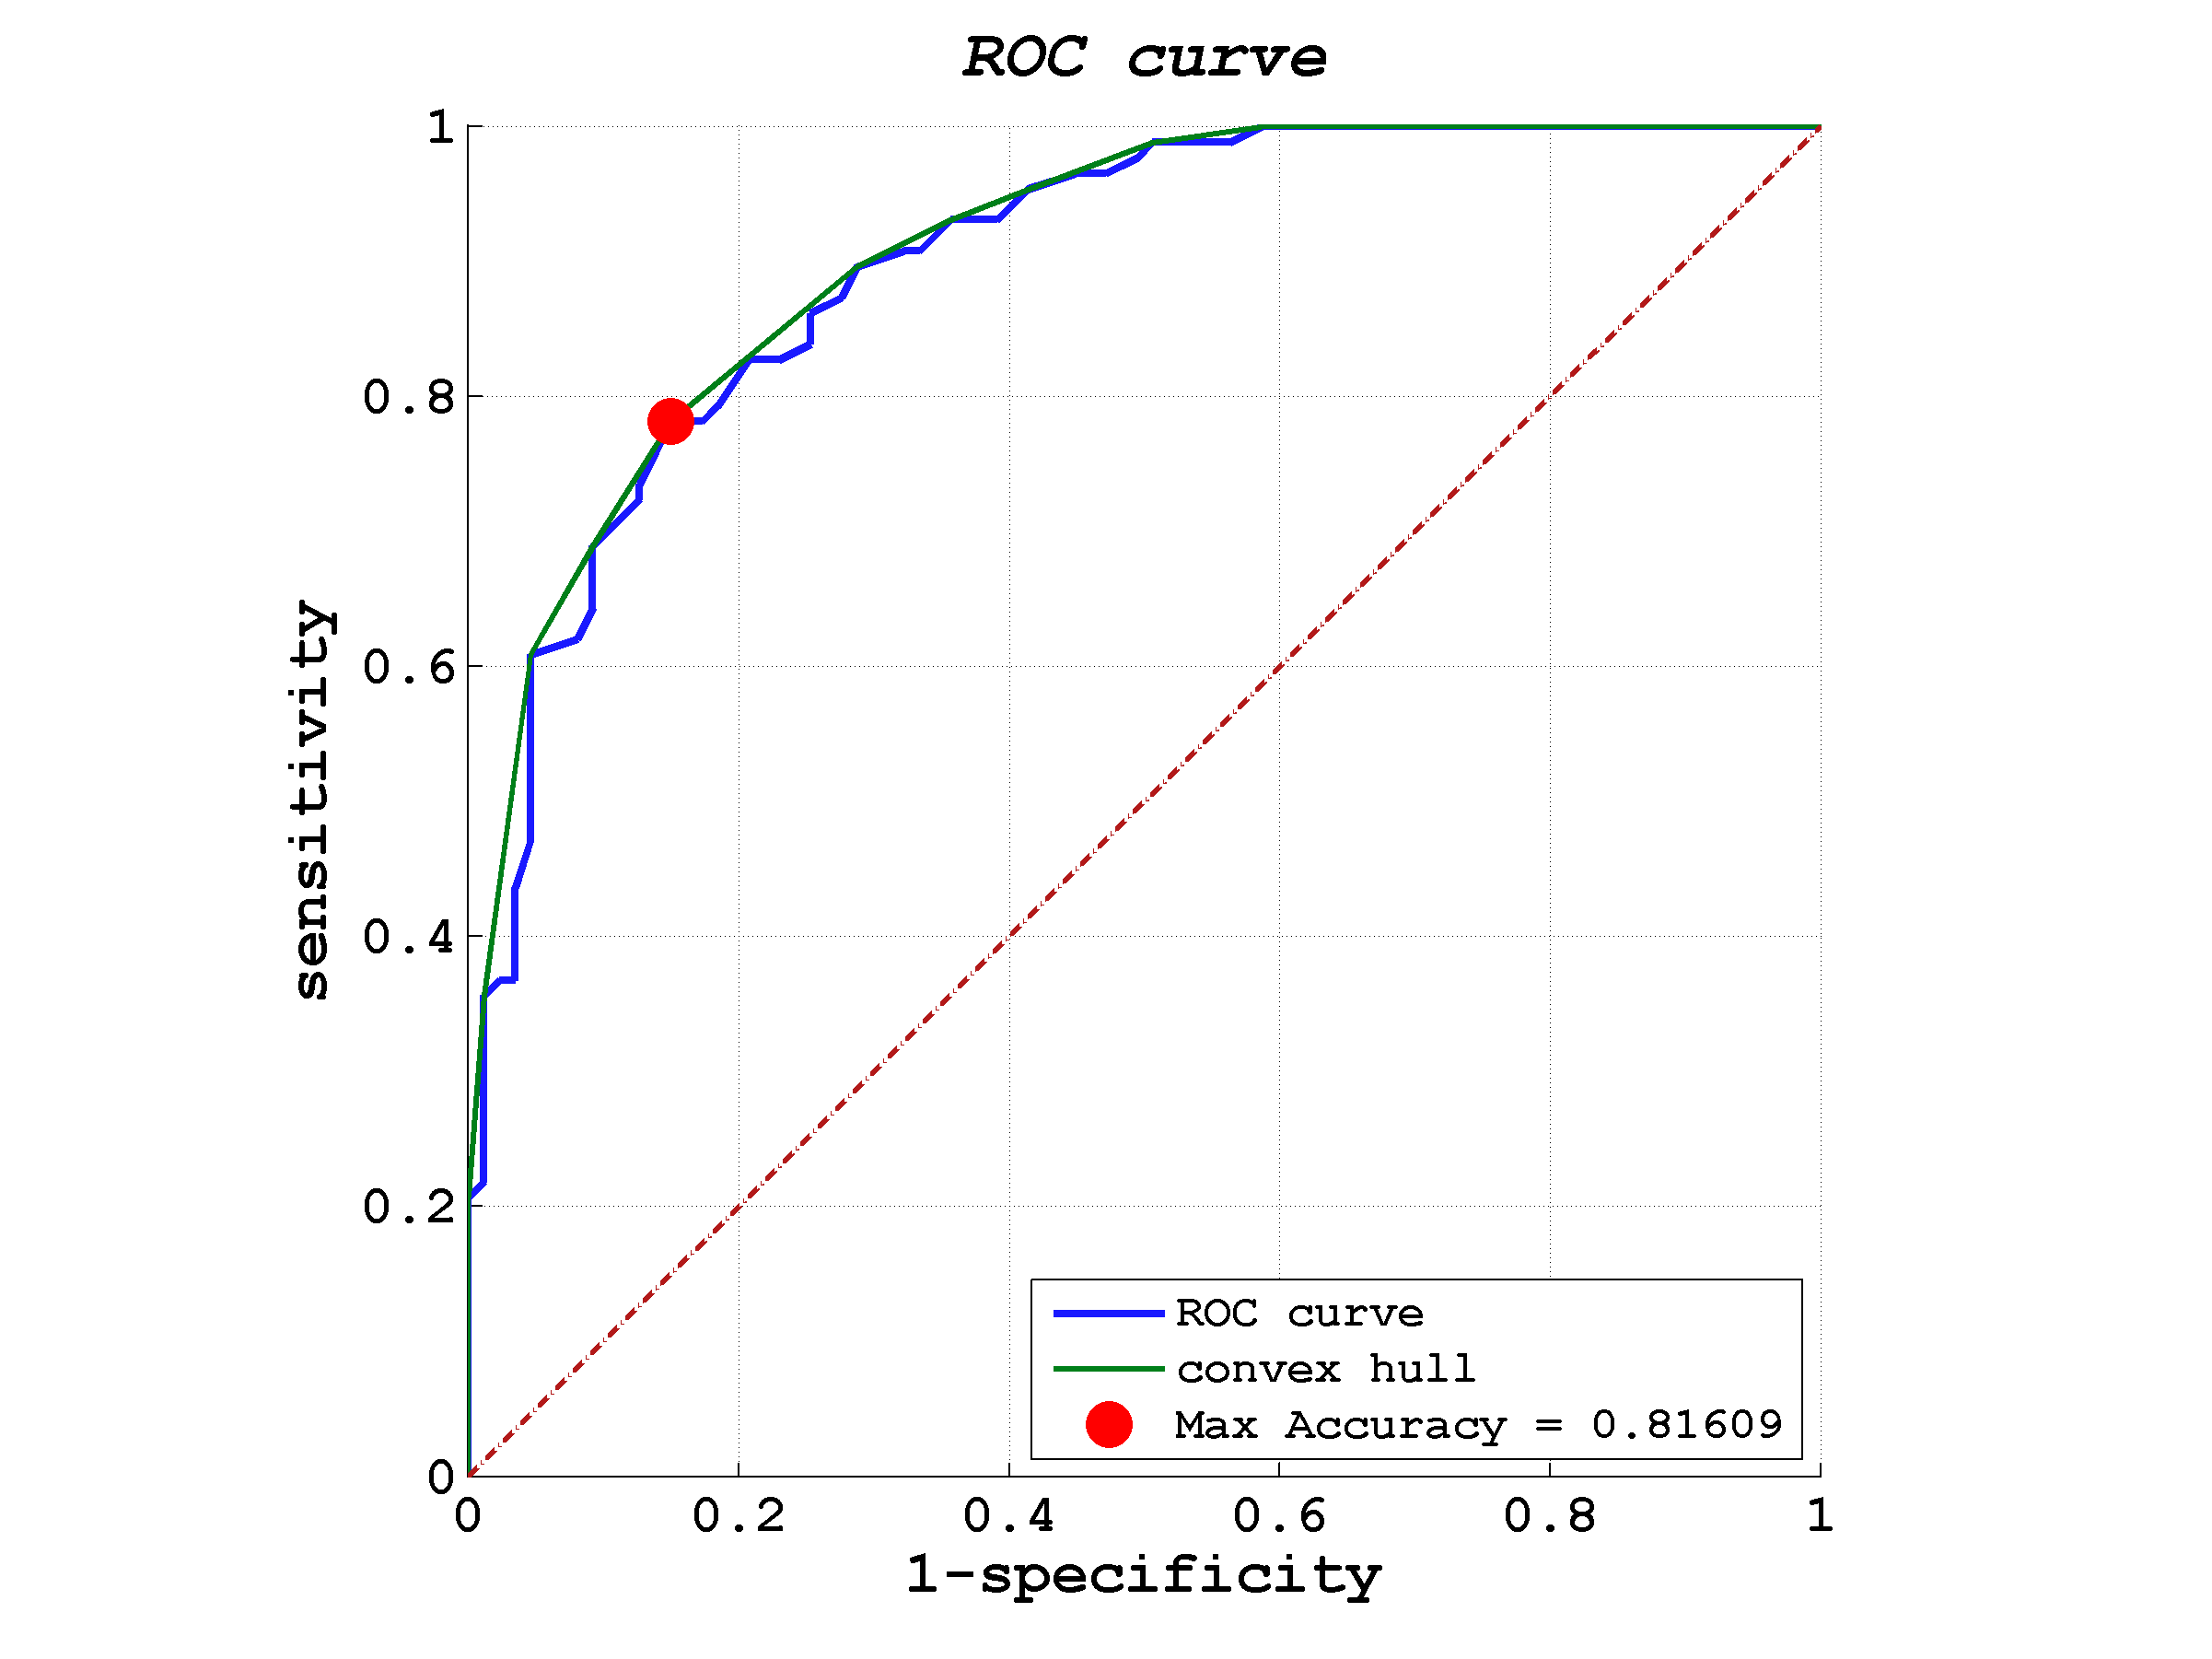
\includegraphics[width=0.46\textwidth]{./images/exp02/RF_MSiHR_extT.png}
      \label{ch6:fig5:b}
    }
    \\
    \subfigure[RF ext-E - ROC]{
      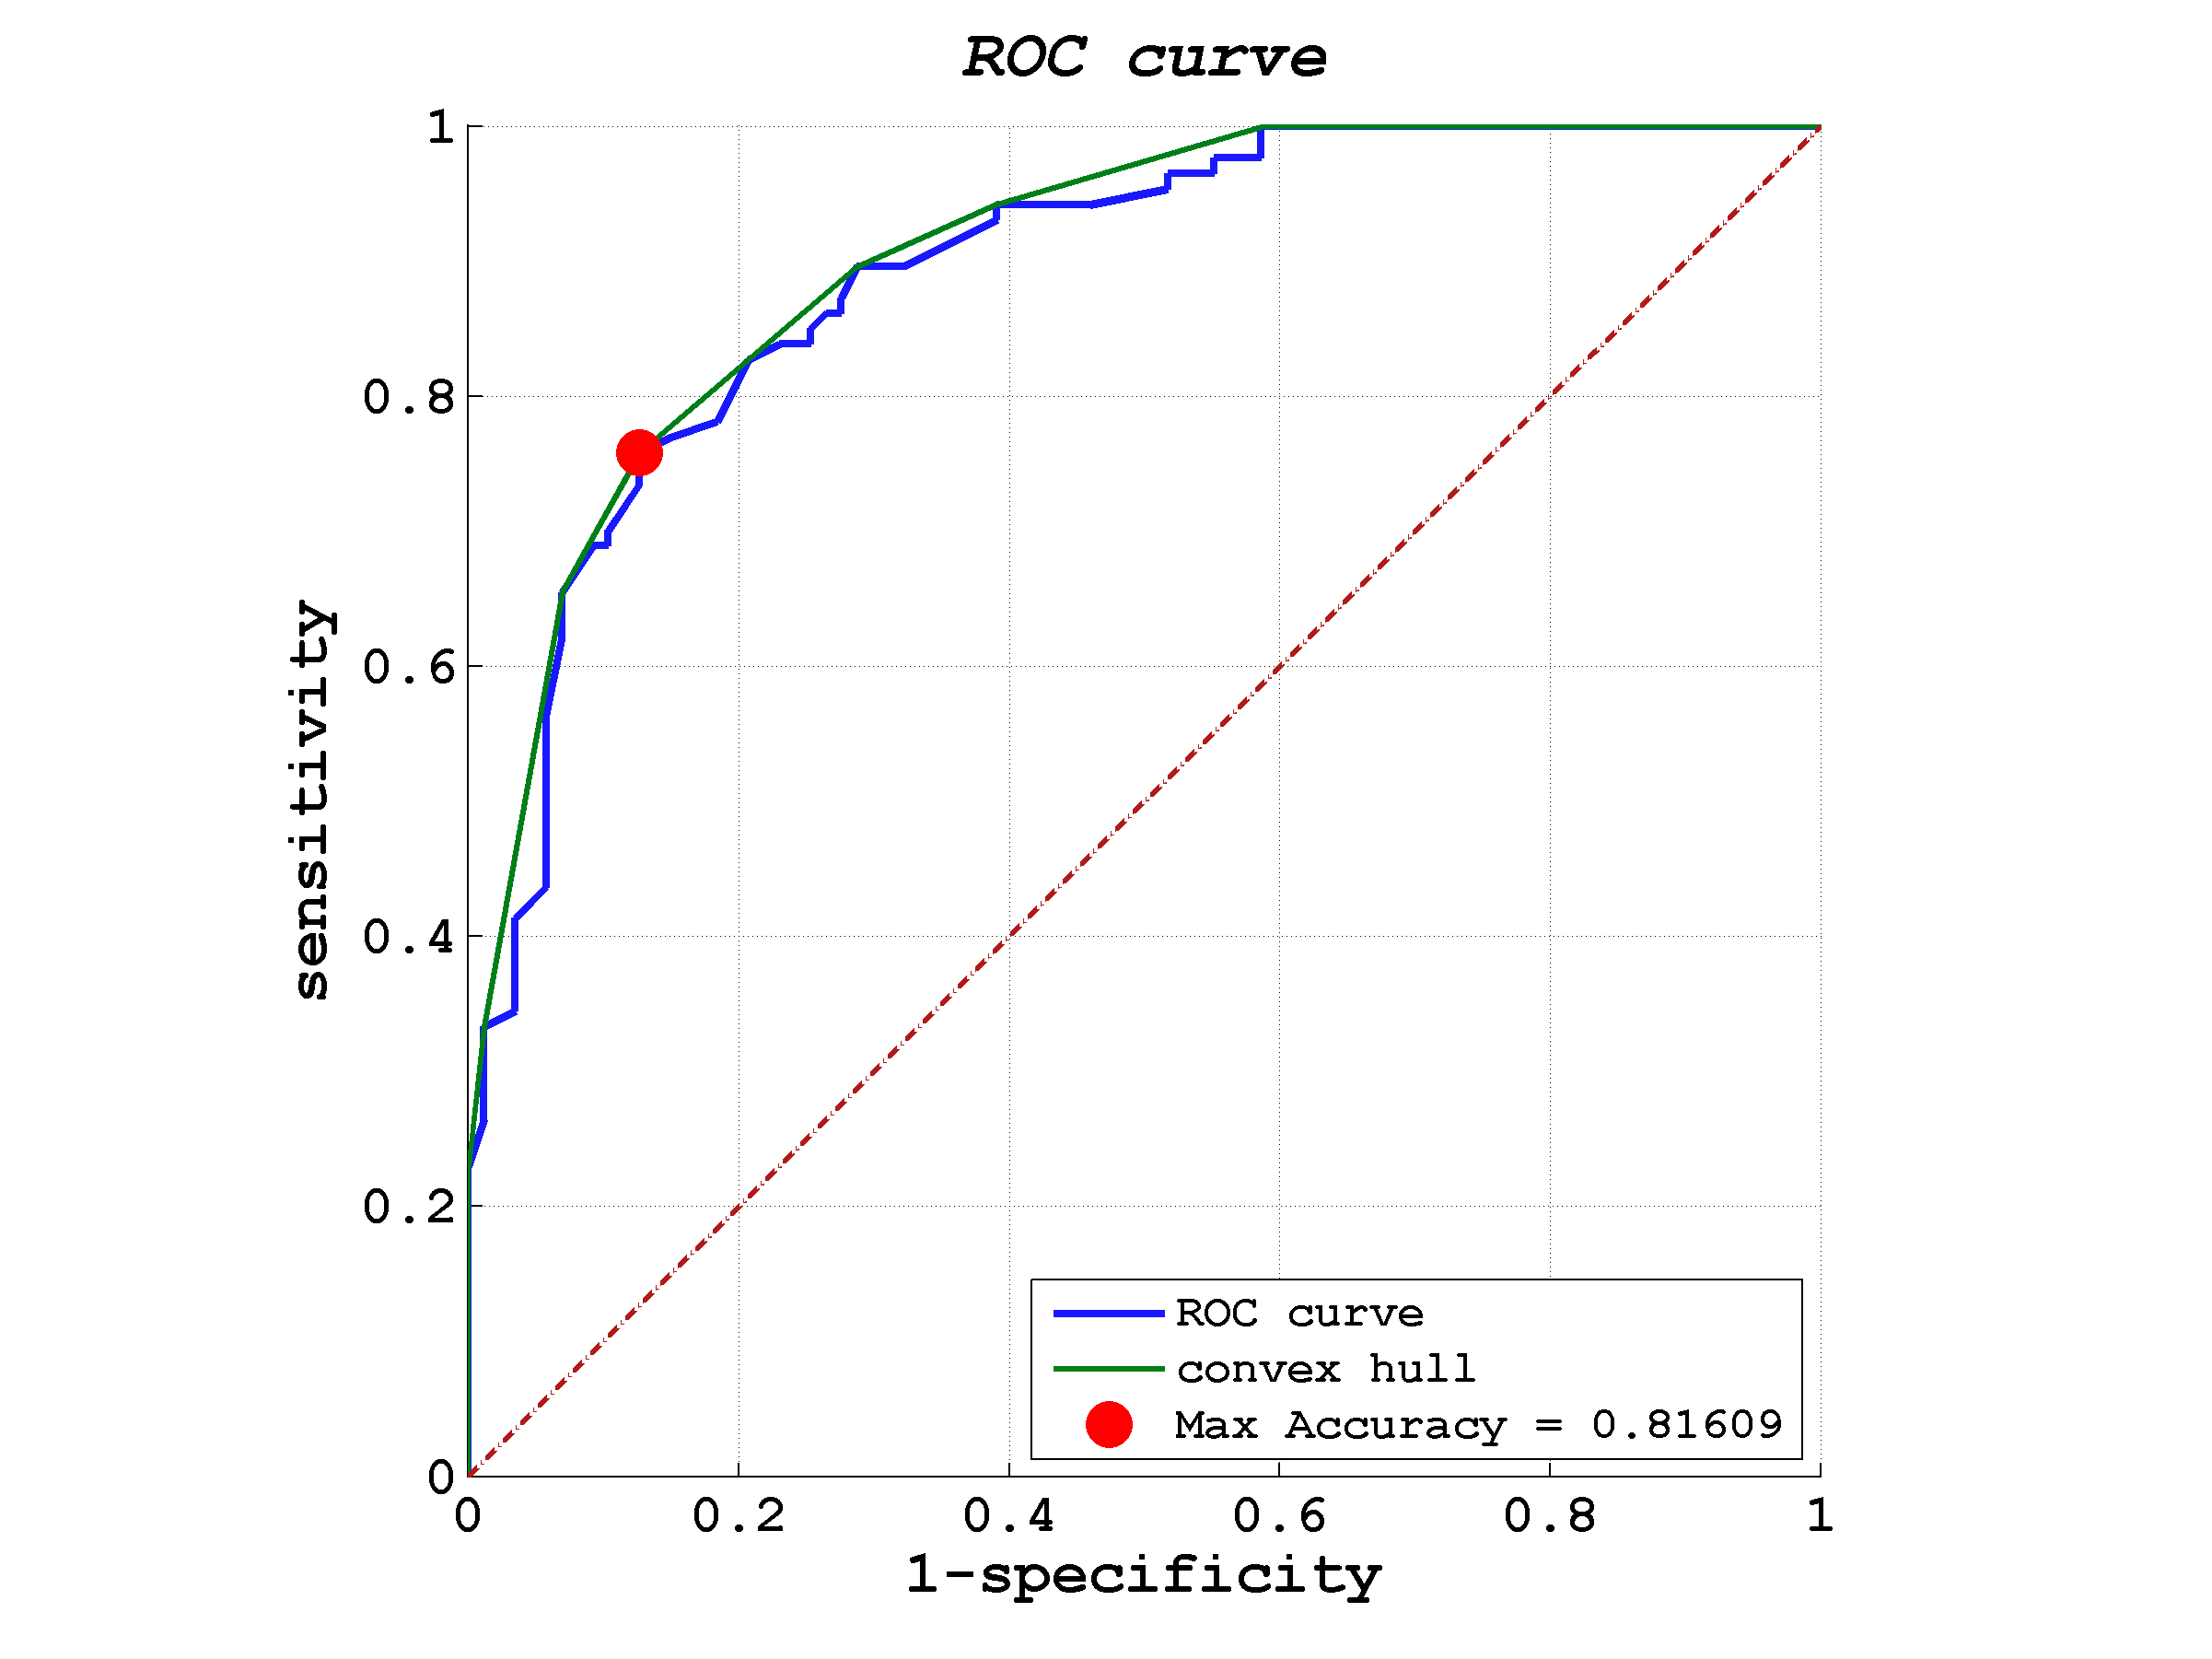
\includegraphics[width=0.46\textwidth]{./images/exp02/RF_MSiHR_extE.png}
      \label{ch6:fig5:c}
    }    
    \hspace{1mm}
    \subfigure[RF ext-A - ROC]{
      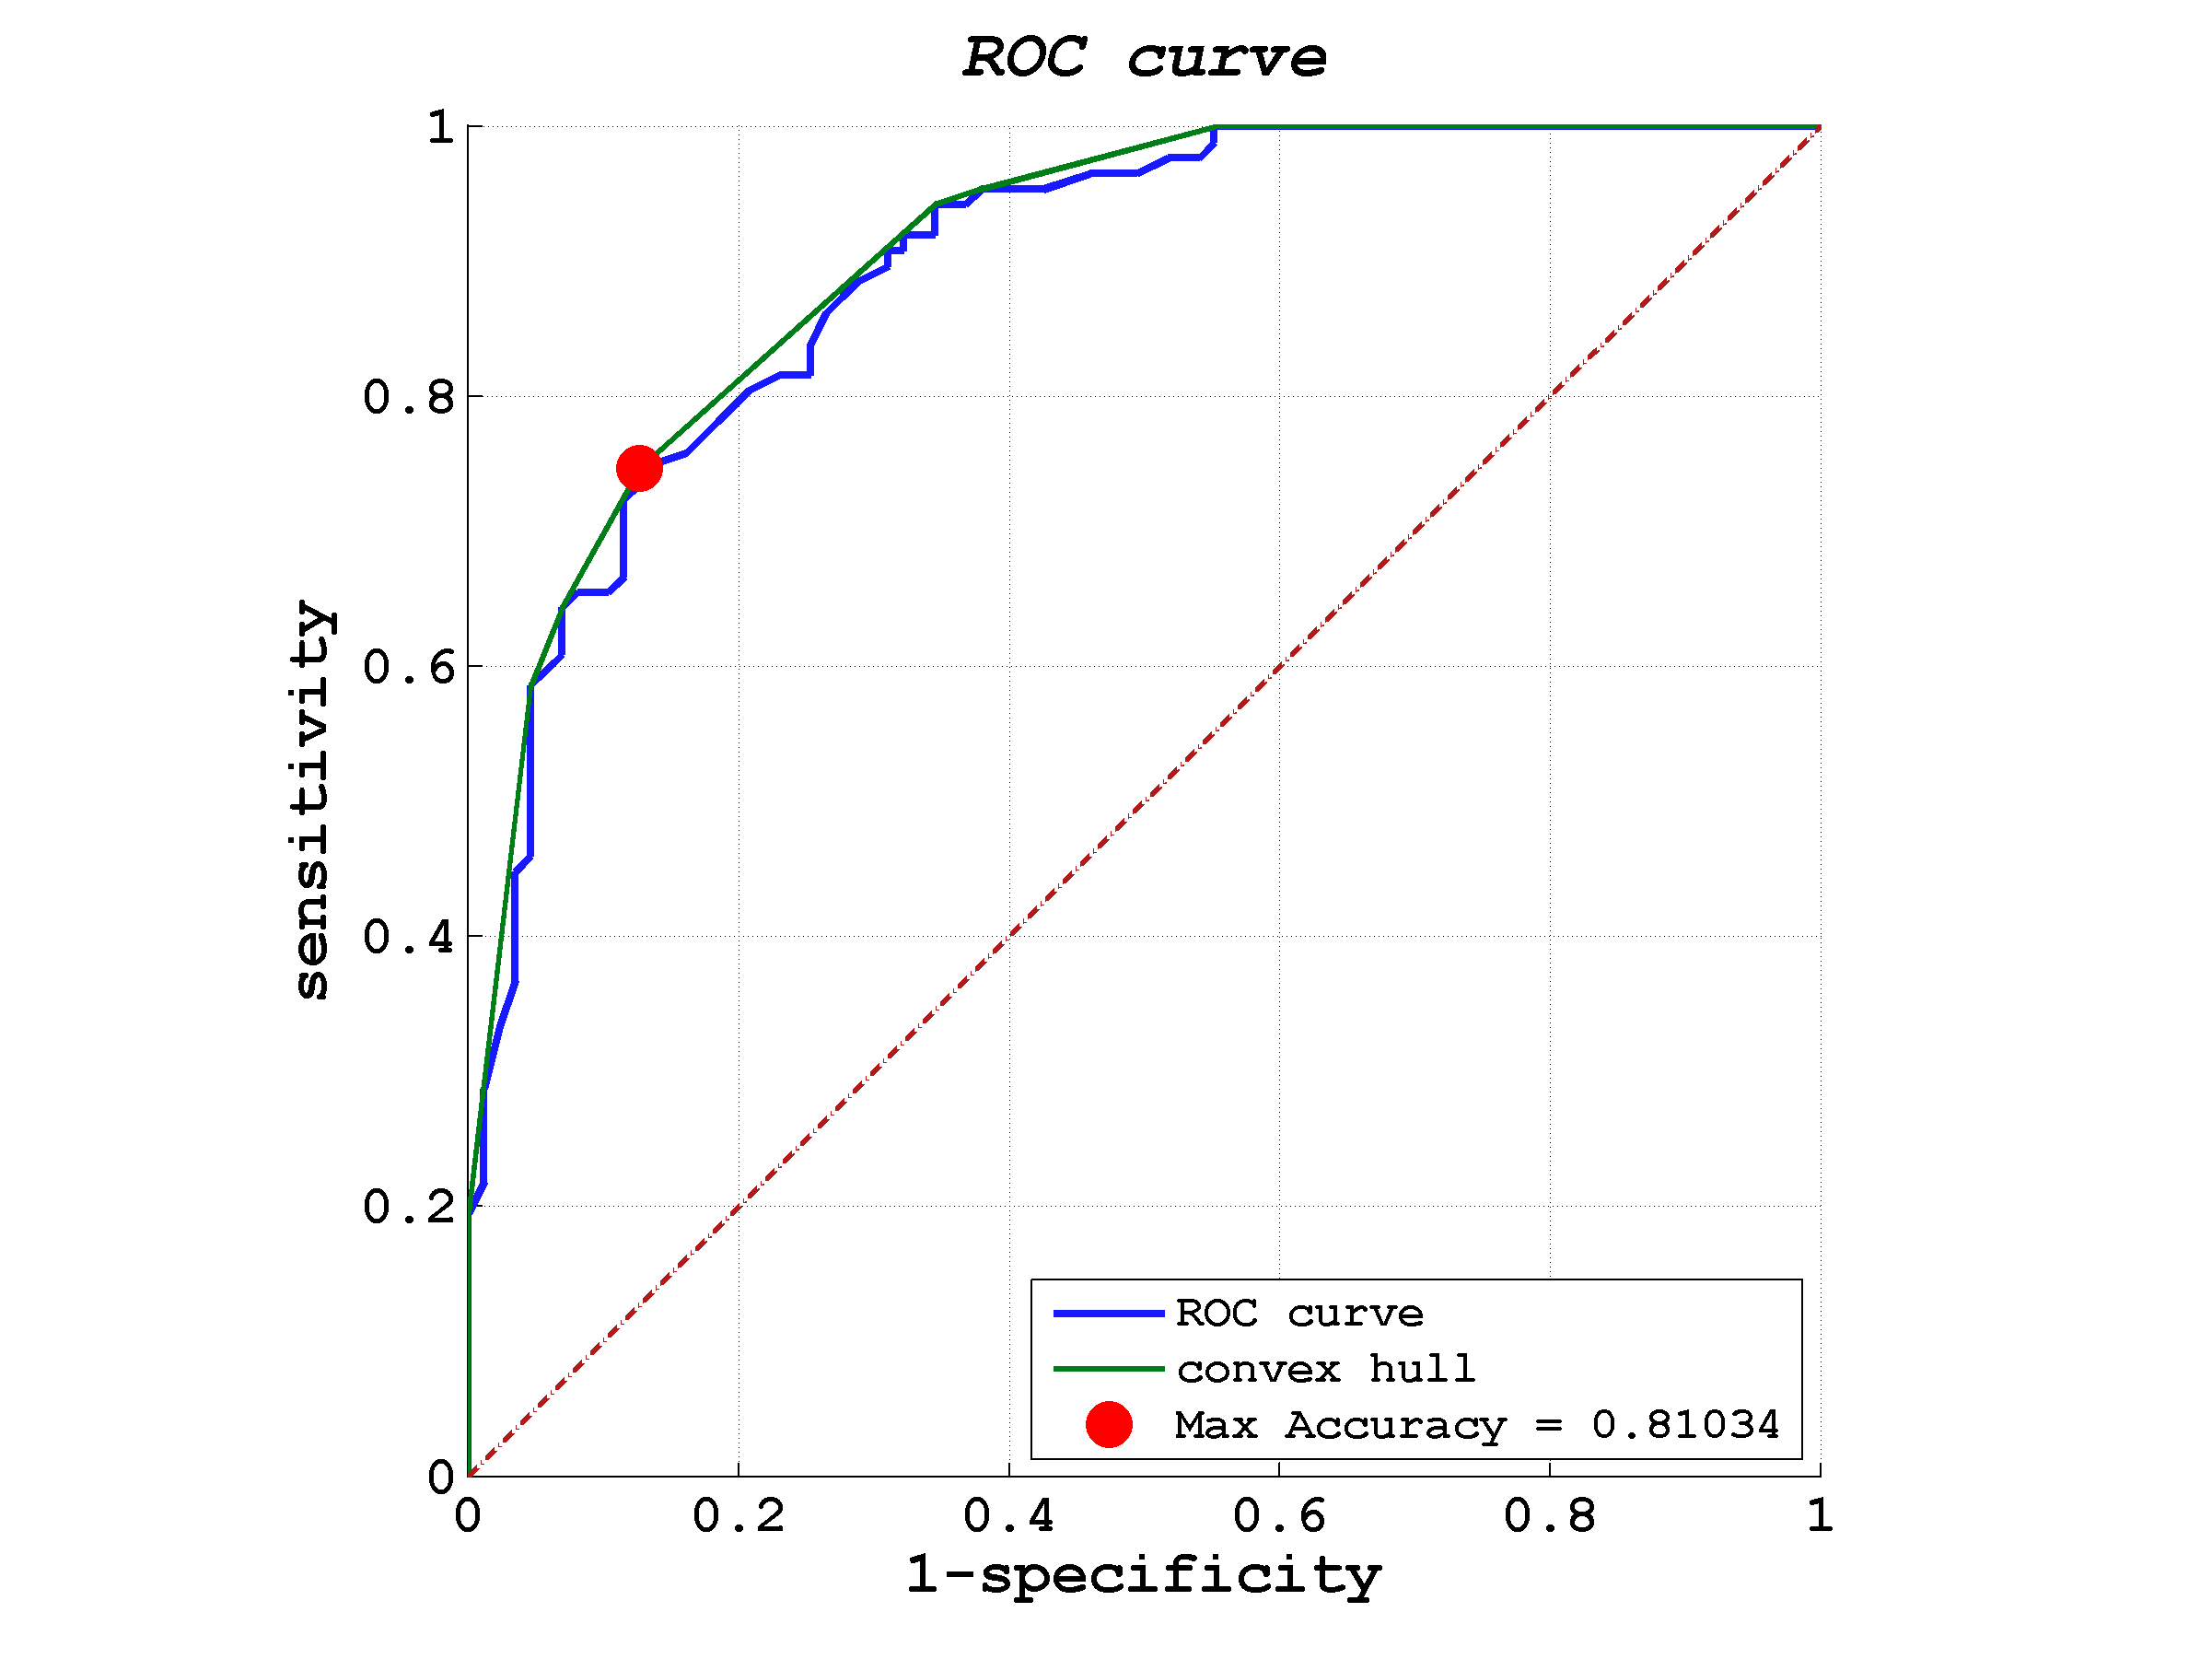
\includegraphics[width=0.46\textwidth]{./images/exp02/RF_MSiHR_extA.png}
      \label{ch6:fig5:d}
    }
    \caption{ROC curves for \texttt{MSiHR} features - RF classification}
    \label{ch6:fig5}
\end{figure}


In the following examples we considered extended datasets, unless explicitly specified.


\vspace{0.5cm}

\subsection{Best Feature Combinations}
\label{ch6:sec_best}

In this experiment we looked for the best combination of features, so we considered all the features described in \ref{ch4:FE}. Having \textit{n} features, maybe multi-component,
they can be combined in $2^n-1$ ways. As the texture features (see Section \ref{ch4:tf}, in particular Equation \ref{ch4:tftypes}) are mutually exclusive, we run three different
experiments, one for each texture feature set.
\\
The Matlab code implemented to run \textit{experiment 3} is listed in \ref{appendixB:exp3}

\vspace{0.5cm}


\subsection{Best Feature Combinations: Experimental Results}


Having run all possible combinations of features, we report here the best performance found, divided for \Gls{RF} and \Gls{SVM} classifiers.

\vspace{0.5cm}

\subsubsection{Best Performances - classifier: SVM}

The four feature sets which gave best results, when classified with \Gls{SVM} are described in Table \ref{ch6:tab9}. The detailed number of classified images,
at the optimal classification threshold is shown in Table \ref{ch6:tab10}.

\begin{table}[!hbt]
\tiny
 \centering
 \begin{tabularx}{350pt}{ l |>{\centering\arraybackslash} X |>{\centering\arraybackslash} X |>{\centering\arraybackslash} X |>{\centering\arraybackslash} X |>{\centering\arraybackslash} X |>{\centering\arraybackslash} X}
   Classifier     & AUC  & accuracy & precision & F$_1$-Score & sensitivity & specificity \\
   \hline
   \hline
    SVM - H      & 0.83 & 79.89\% & 73.21\% & 0.82 & 65.52\% & \cellcolor{YellowGreen} 94.25\%  \\
    \hline
    SVM - MSiVH     & 0.85 & 78.74\% & \cellcolor{YellowGreen} 87.88\% & 0.76 & \cellcolor{YellowGreen} 90.80\% & 66.67\%  \\
    \hline
    SVM - SiU     & \cellcolor{YellowGreen} 0.88 & \cellcolor{YellowGreen} 84.48\% & 81.91\% & \cellcolor{YellowGreen} 0.85 & 80.46\% & 88.51\%  \\
    \hline
    SVM - SiVHU     & \cellcolor{YellowGreen} 0.88 & 80.46\% & 77.32\% & 0.82 & 74.71\% & 86.21\% \\
    \hline
 \end{tabularx}
 \caption{Best SVM results}
 \label{ch6:tab9}
\end{table}

\begin{table}[!hbt]
\tiny
 \centering
 \begin{tabularx}{320pt}{ l |>{\centering\arraybackslash} X |>{\centering\arraybackslash} X |>{\centering\arraybackslash} X |>{\centering\arraybackslash} X }
   Classifier     & TP  & FN & TN & FP  \\
   \hline
   \hline
    SVM - H      & \cellcolor{YellowGreen} 82 & 5 & 57 & 30  \\
    \hline
    SVM - MSiVH     & 58 & 29 & \cellcolor{YellowGreen} 79 & 8  \\
    \hline
    SVM - SiU     & 77 & 10 & 70 & 17  \\
    \hline
    SVM - SiVHU     & 75 & 12 & 65 & 22 \\
    \hline
    \end{tabularx}
 \caption{Best SVM results - classified images}
 \label{ch6:tab10}
\end{table}  


The \Gls{ROC} curves of these classifications are shown in Figure \ref{ch6:fig6}.

\begin{figure}[!htb]
  \centering
    \subfigure[SVM H - ROC]{
      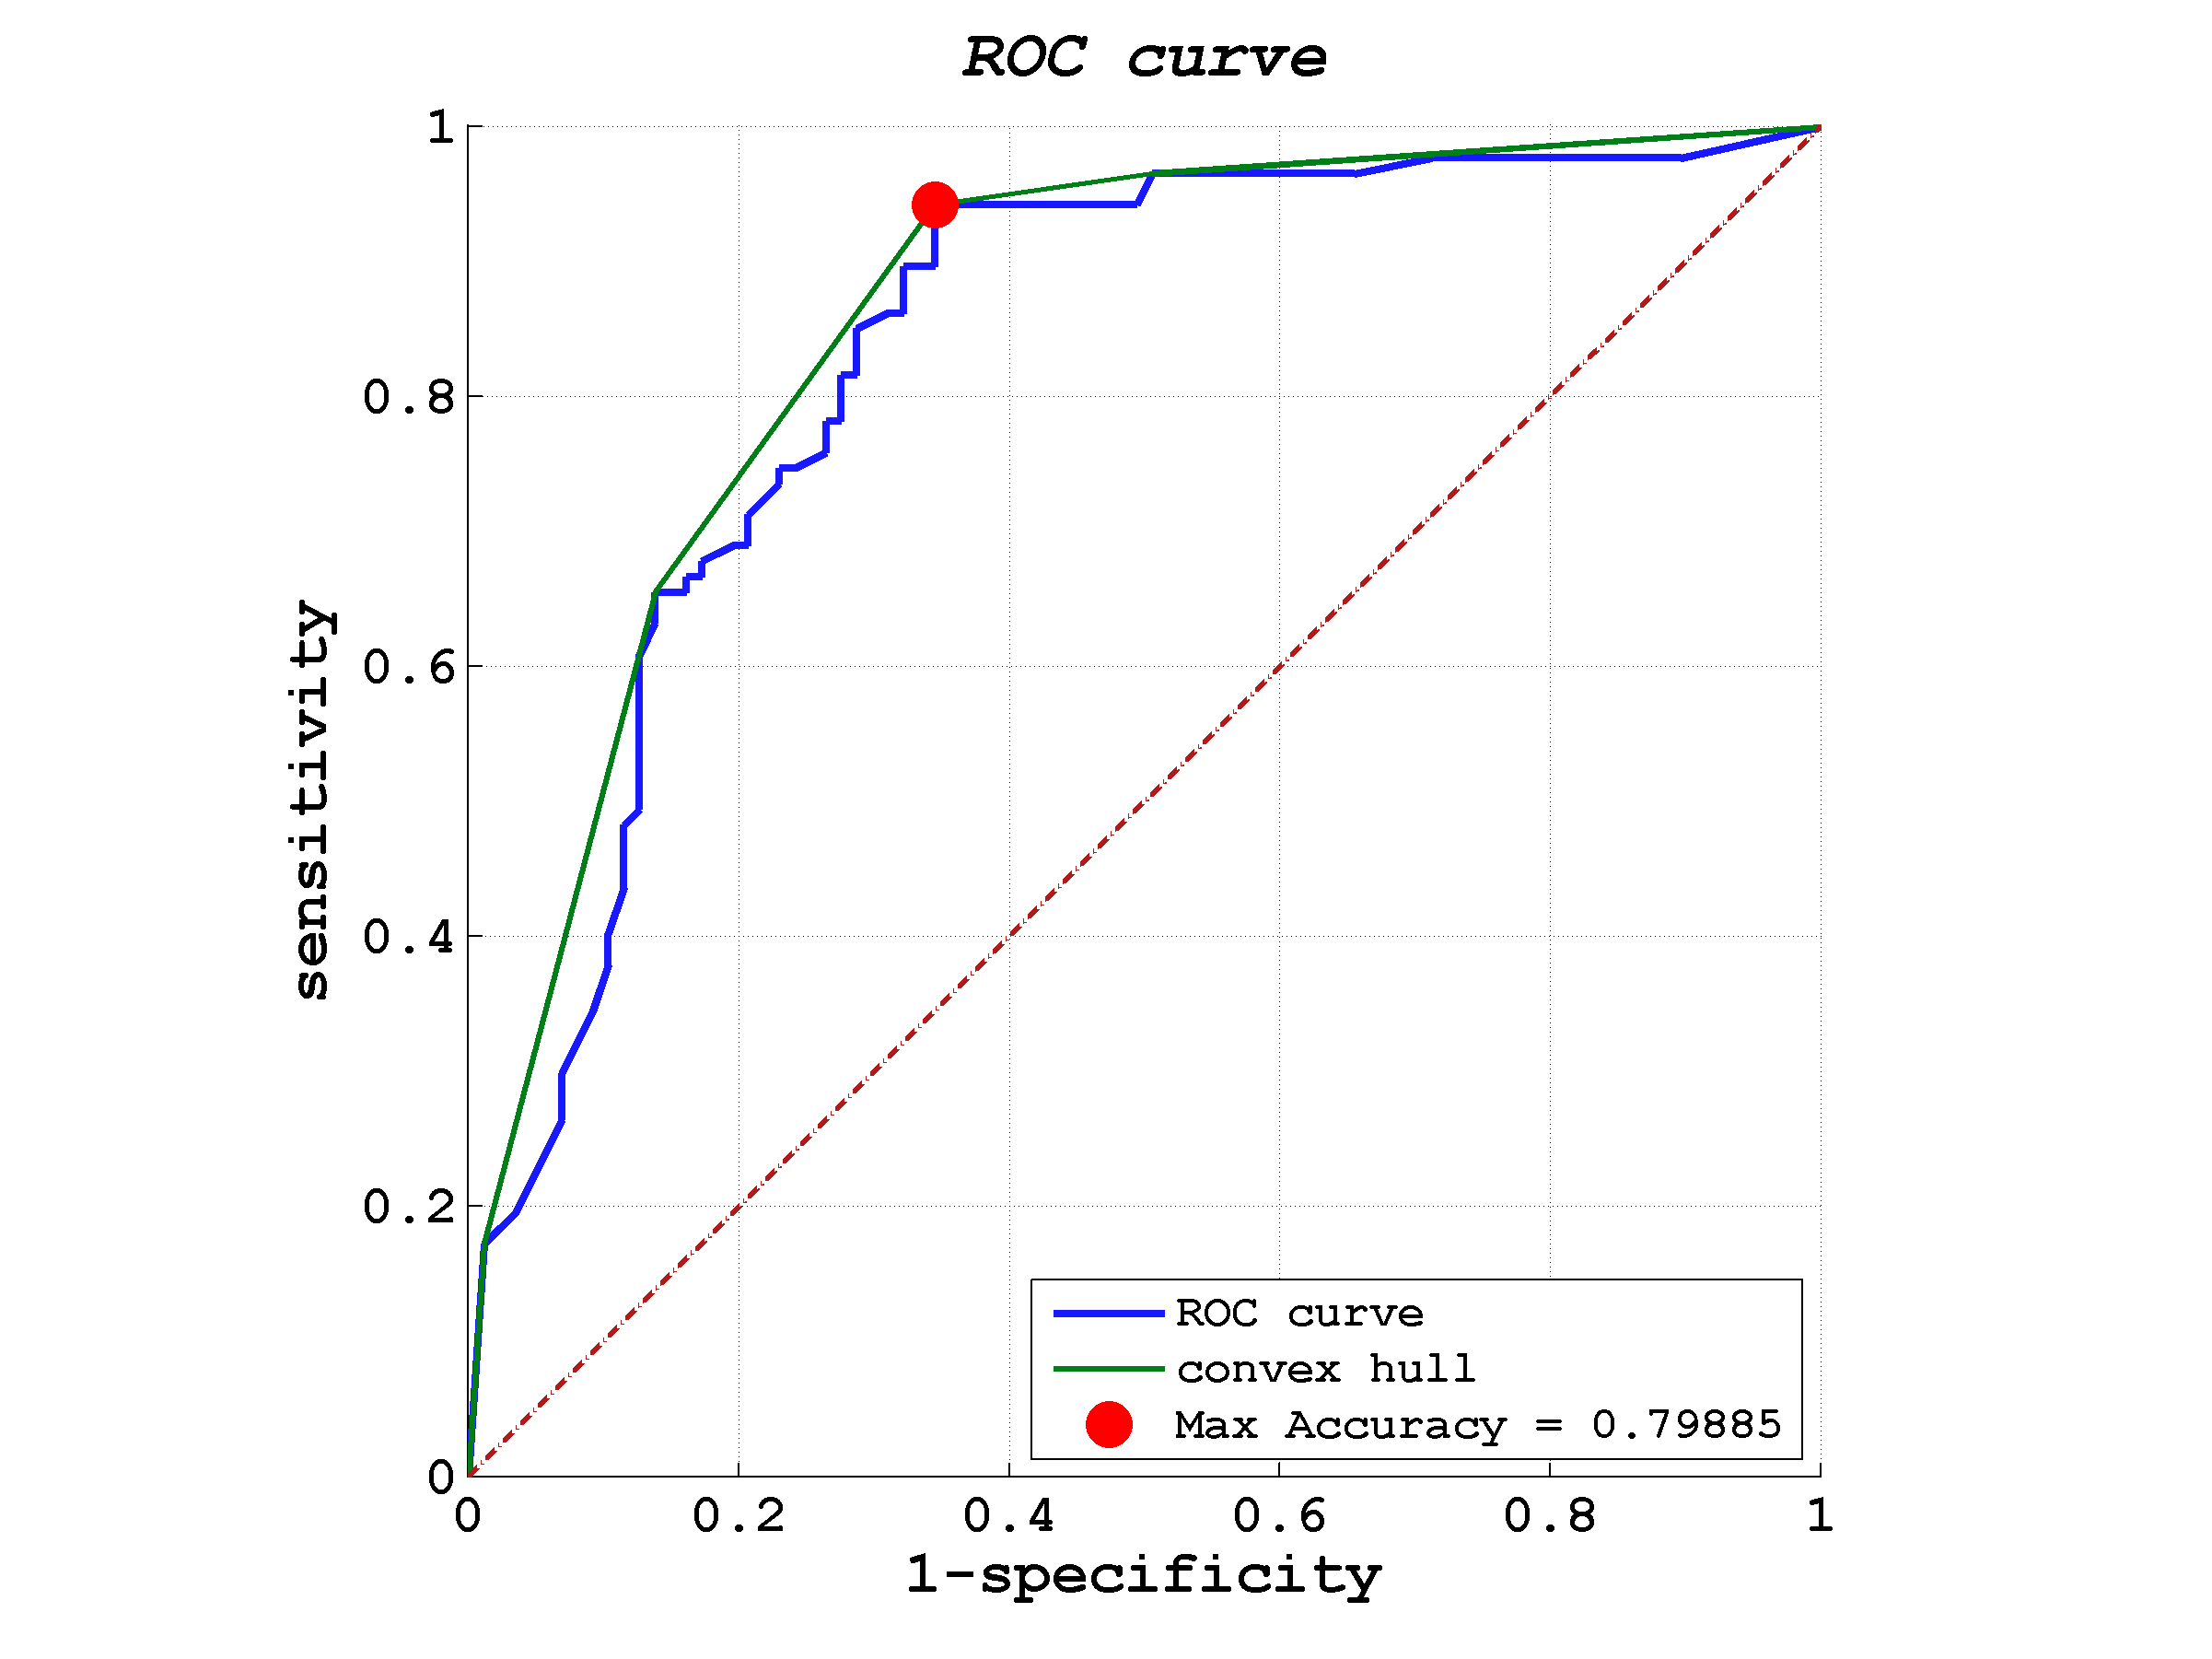
\includegraphics[width=0.46\textwidth]{./images/exp03/class/SVMprob_H_extA.png}
      \label{ch6:fig6:a}
    }
    \hspace{1mm}
    \subfigure[SVM MSiVH - ROC]{
      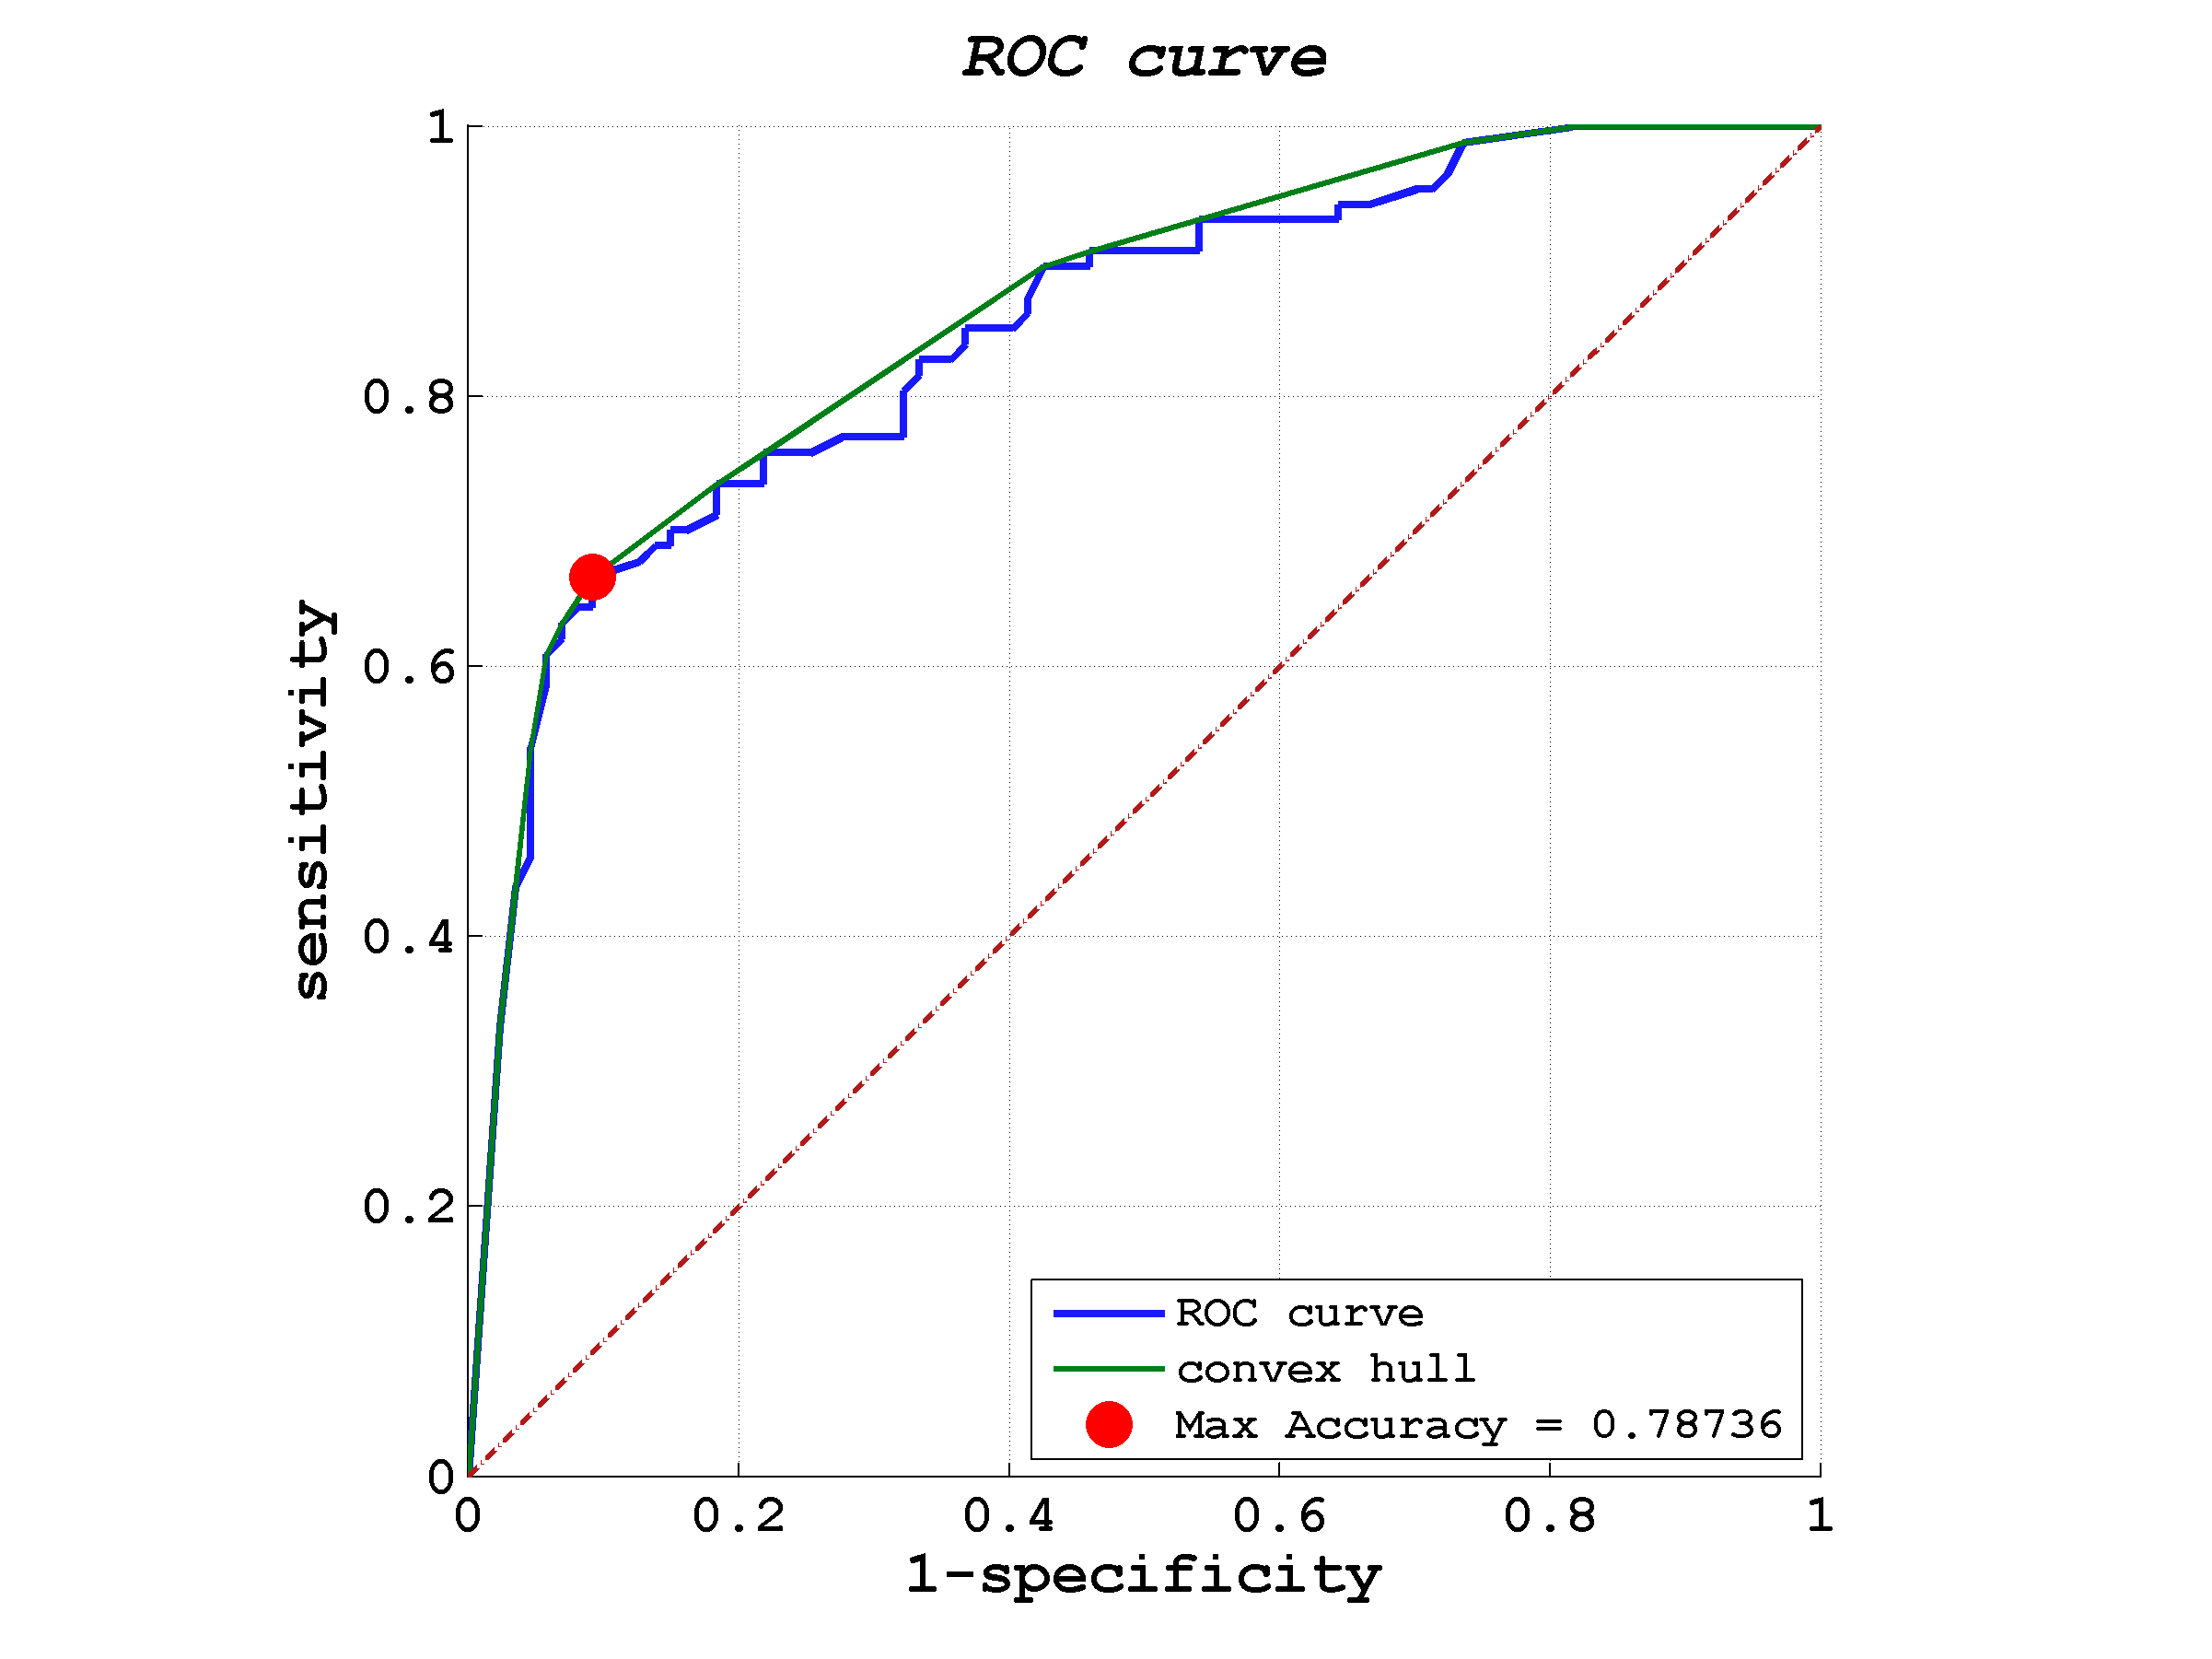
\includegraphics[width=0.46\textwidth]{./images/exp03/class/SVMprob_MSiVH_extA.png}
      \label{ch6:fig6:b}
    }
    \\
    \subfigure[SVM SiU - ROC]{
      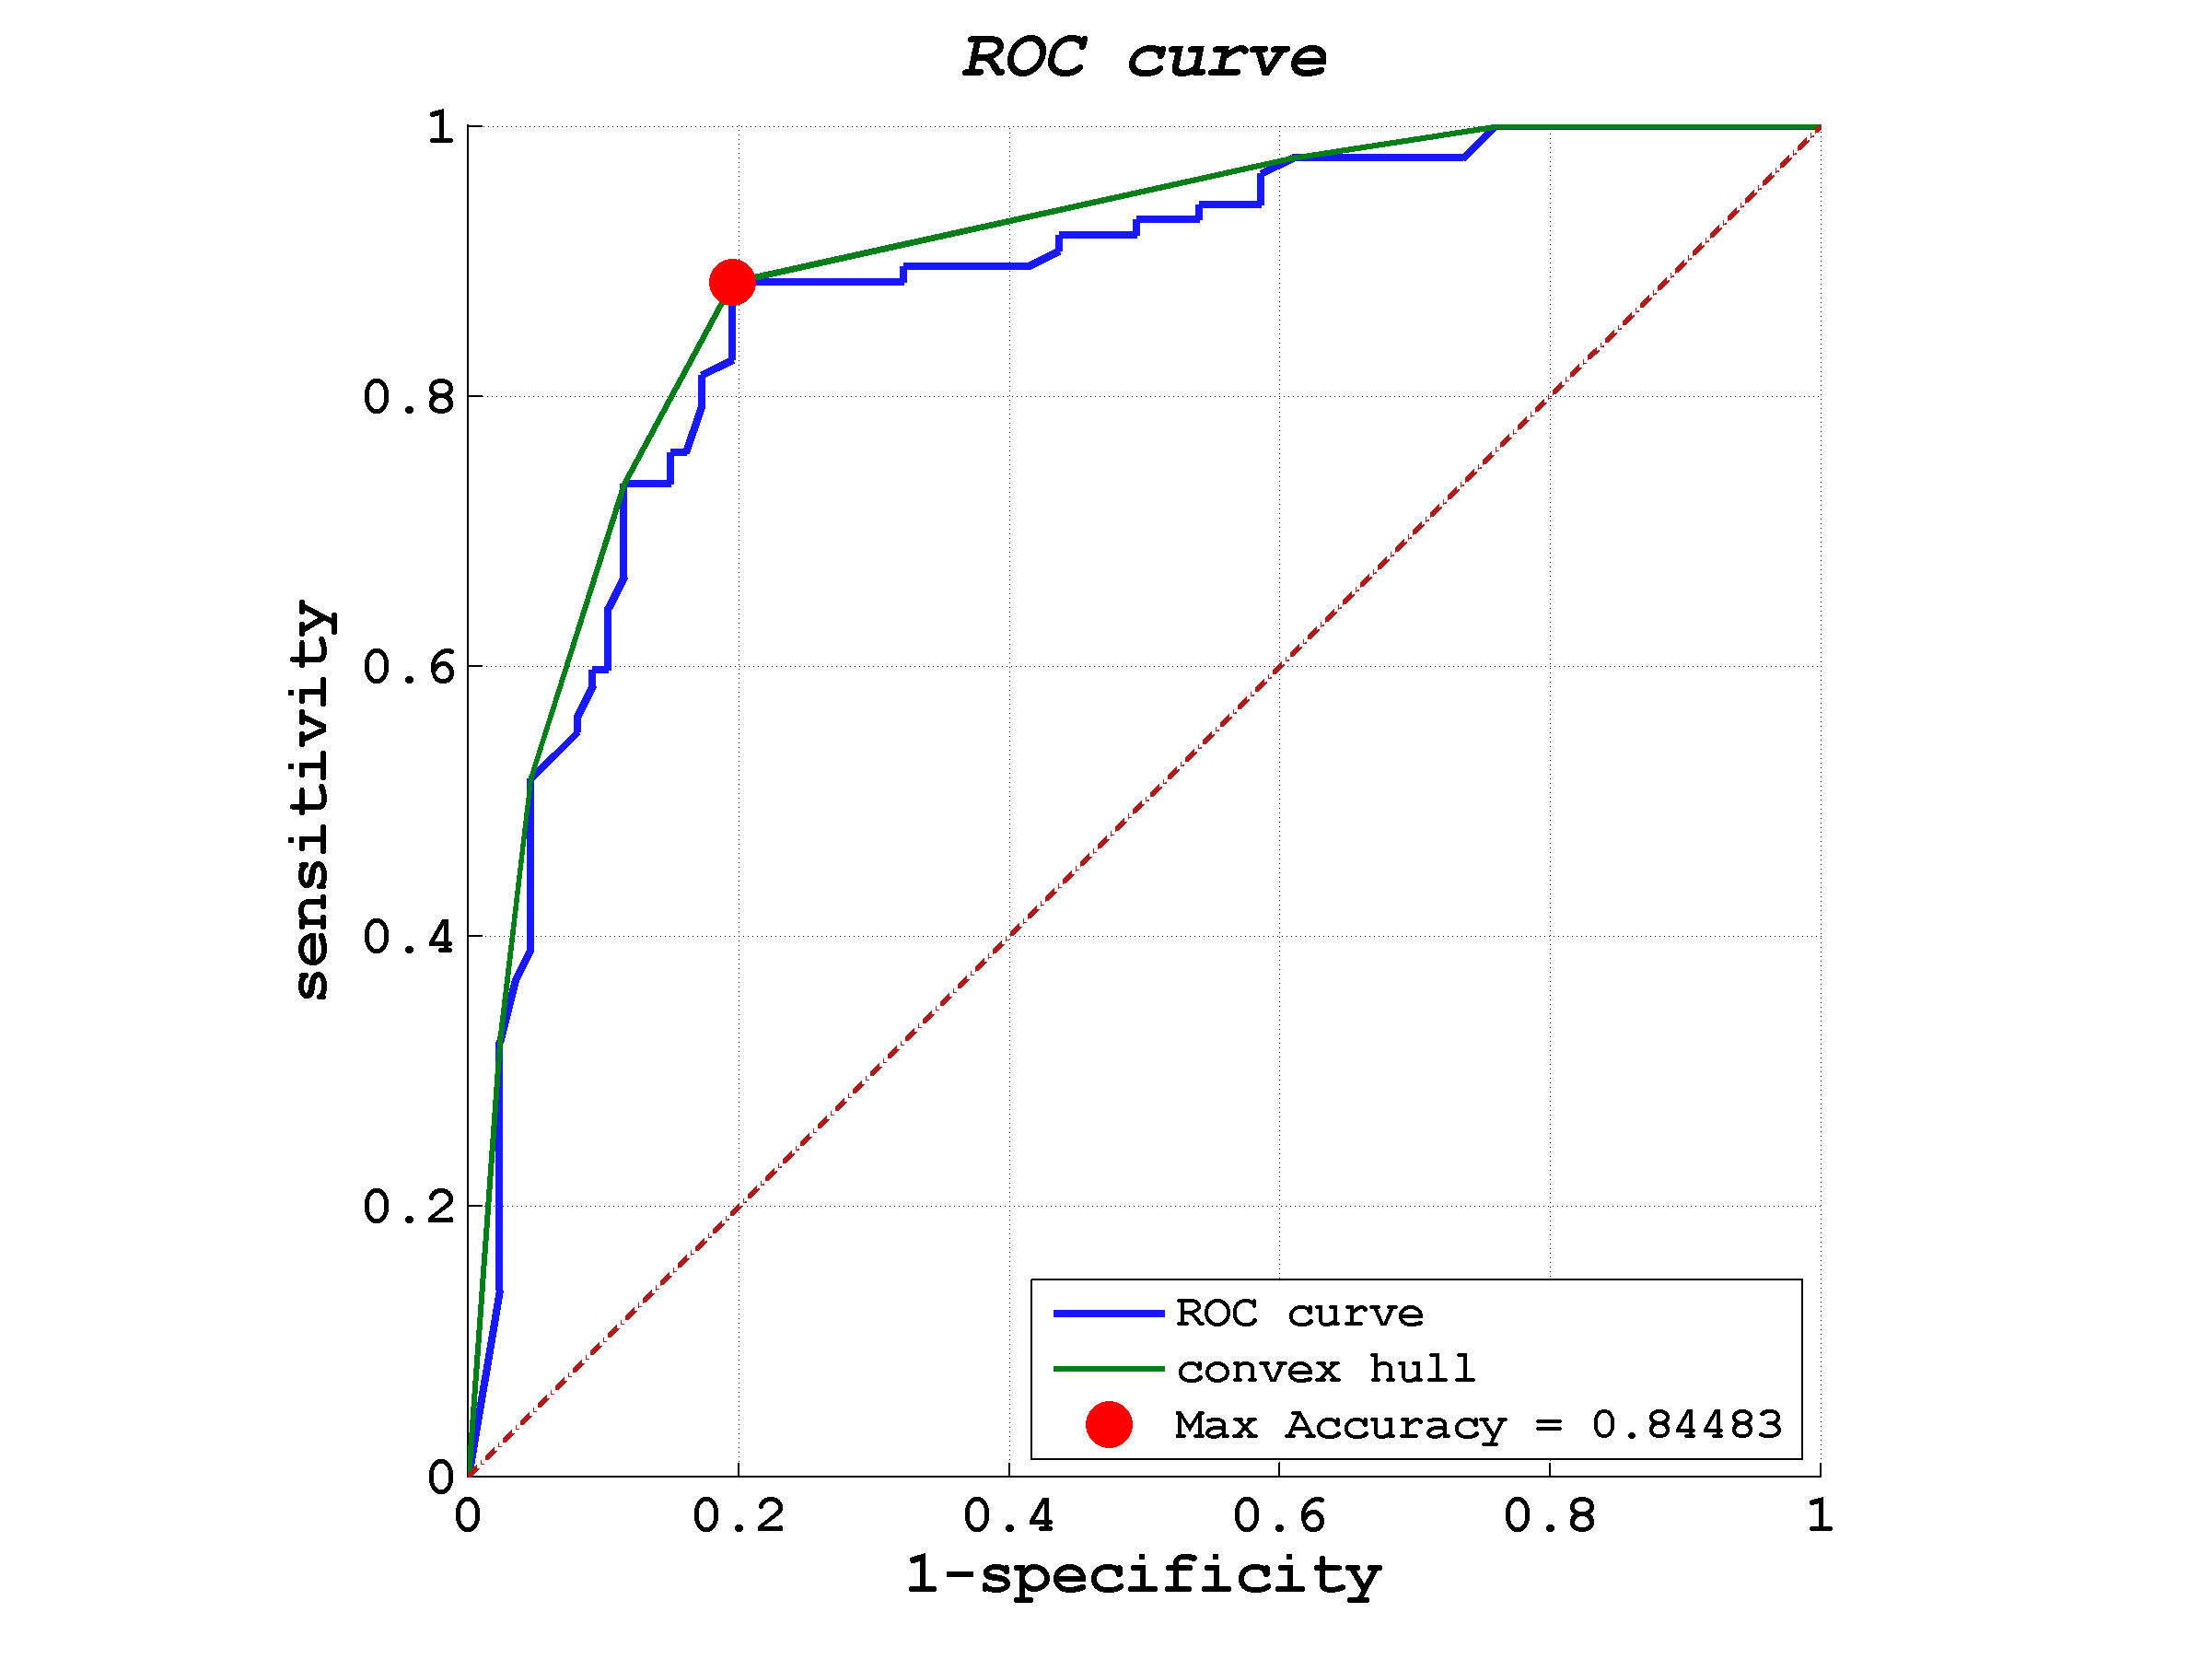
\includegraphics[width=0.46\textwidth]{./images/exp03/class/SVMprob_SiU_extA.png}
      \label{ch6:fig6:c}
    }    
    \hspace{1mm}
    \subfigure[SVM SiVHU - ROC]{
      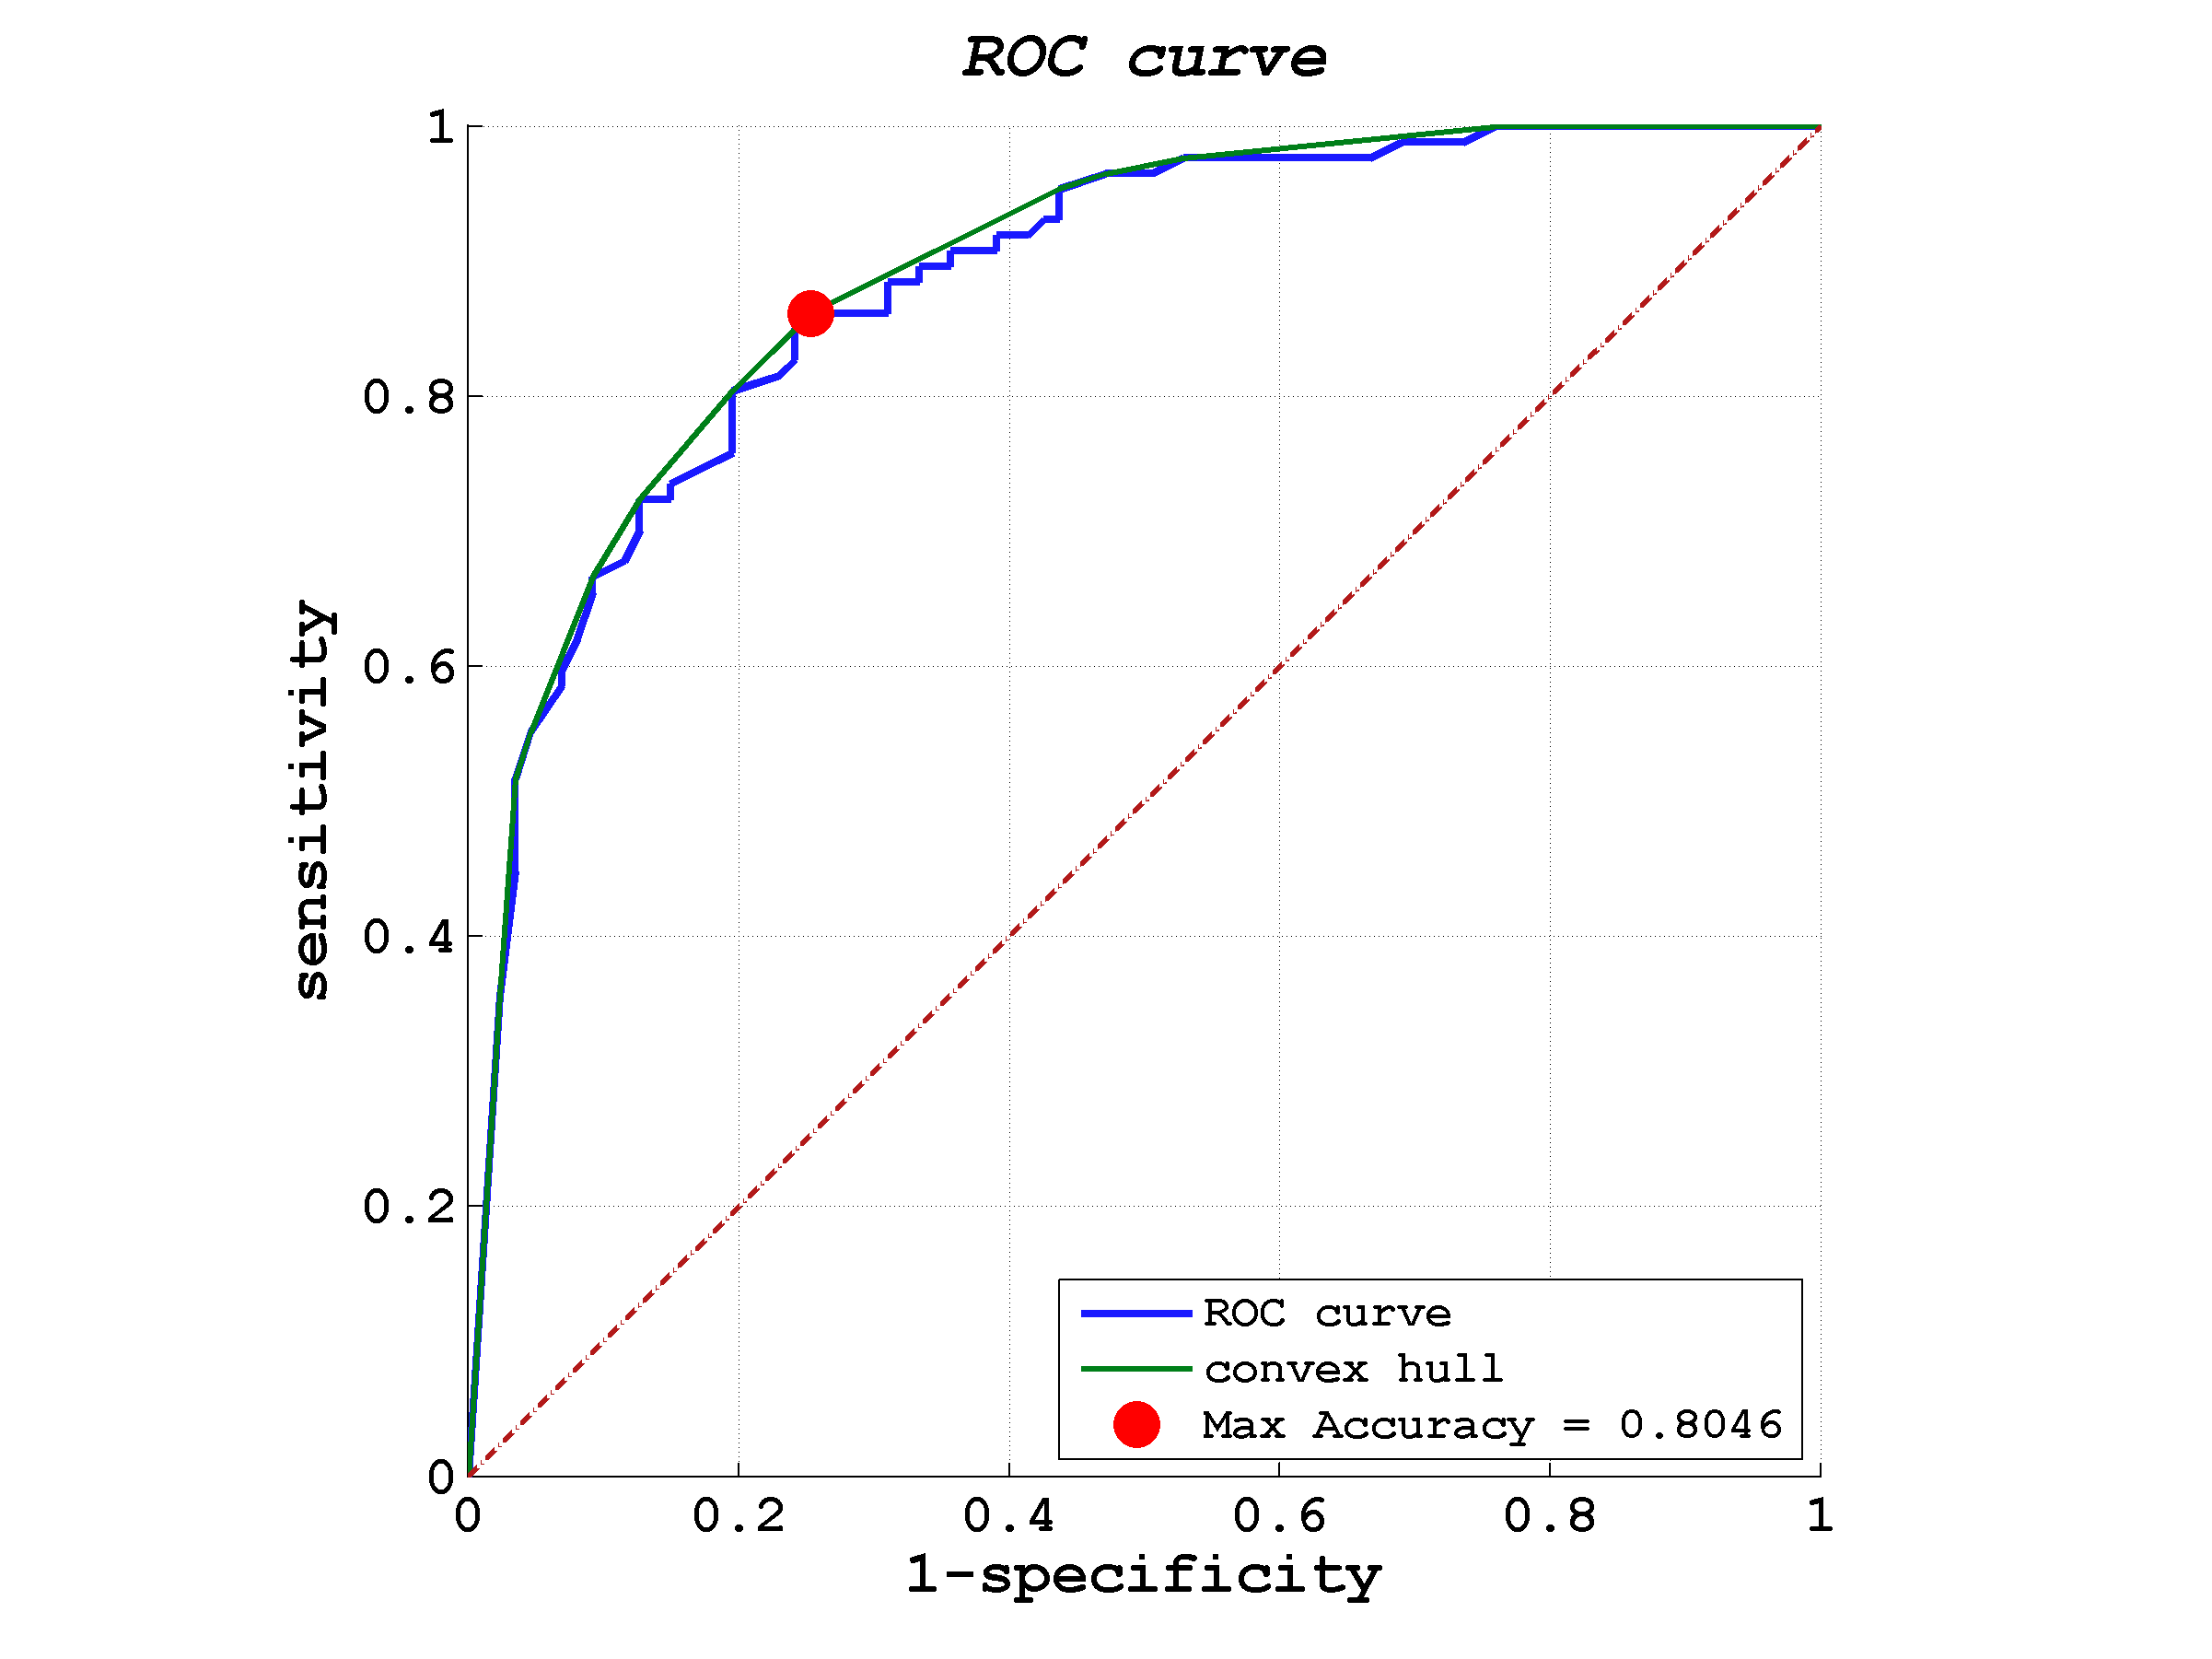
\includegraphics[width=0.46\textwidth]{./images/exp03/class/SVMprob_SiVHU_extA.png}
      \label{ch6:fig6:d}
    }
    \caption{ROC curves for best feature-set - SVM classification}
    \label{ch6:fig6}
\end{figure}

\vspace{0.5cm}

\subsubsection{Best Performances - classifier: RF}

The four feature sets which gave best results, when classified with \Gls{RF} are described in Table \ref{ch6:tab11}. The detailed number of classified images,
at the optimal classification threshold is shown in Table \ref{ch6:tab12}.

\begin{table}[!hbt]
\tiny
 \centering
 \begin{tabularx}{350pt}{ l |>{\centering\arraybackslash} X |>{\centering\arraybackslash} X |>{\centering\arraybackslash} X |>{\centering\arraybackslash} X |>{\centering\arraybackslash} X |>{\centering\arraybackslash} X}
   Classifier     & AUC  & accuracy & precision & F$_1$-Score & sensitivity & specificity \\
   \hline
   \hline
    RF - iVHL      &  0.90 & \cellcolor{YellowGreen} 83.91\% & 79.80\% & \cellcolor{YellowGreen} 0.85 & 77.01\% & 90.80\%  \\
    \hline
    RF - MSHL     & 0.89 & 81.03\% & \cellcolor{YellowGreen} 89.71\% & 0.79 & \cellcolor{YellowGreen} 91.95\% & 70.11\%  \\
    \hline
    RF - MSiVHR     & \cellcolor{YellowGreen} 0.91 & \cellcolor{YellowGreen} 83.91\% & 81.05\% & 0.85 & 79.31\% & 88.51\%  \\
    \hline
    RF - SHL     & 0.89 & 80.46\% & 73.04\% & 0.83 & 64.37\% & \cellcolor{YellowGreen} 96.55\% \\
    \hline
 \end{tabularx}
 \caption{Best RF results}
 \label{ch6:tab11}
\end{table}



\begin{table}[!hbt]
\tiny
 \centering
 \begin{tabularx}{320pt}{ l |>{\centering\arraybackslash} X |>{\centering\arraybackslash} X |>{\centering\arraybackslash} X |>{\centering\arraybackslash} X }
   Classifier     & TP  & FN & TN & FP  \\
   \hline
   \hline
    RF - iVHL      & 79 & 8 & 67 & 20  \\
    \hline
    RF - MSHL     & 61 & 26 & \cellcolor{YellowGreen} 80 & 7  \\
    \hline
    RF - MSiVHR     & 77 & 10 & 69 & 18  \\
    \hline
    RF - SHL     & \cellcolor{YellowGreen} 84 & 3 & 56 & 31 \\
    \hline
 \end{tabularx}
 \caption{Best RF results - classified images}
 \label{ch6:tab12}
\end{table}  


The \Gls{ROC} curves of these classifications are shown in Figure \ref{ch6:fig7}.

\begin{figure}[!htb]
  \centering
    \subfigure[RF iVHL - ROC]{
      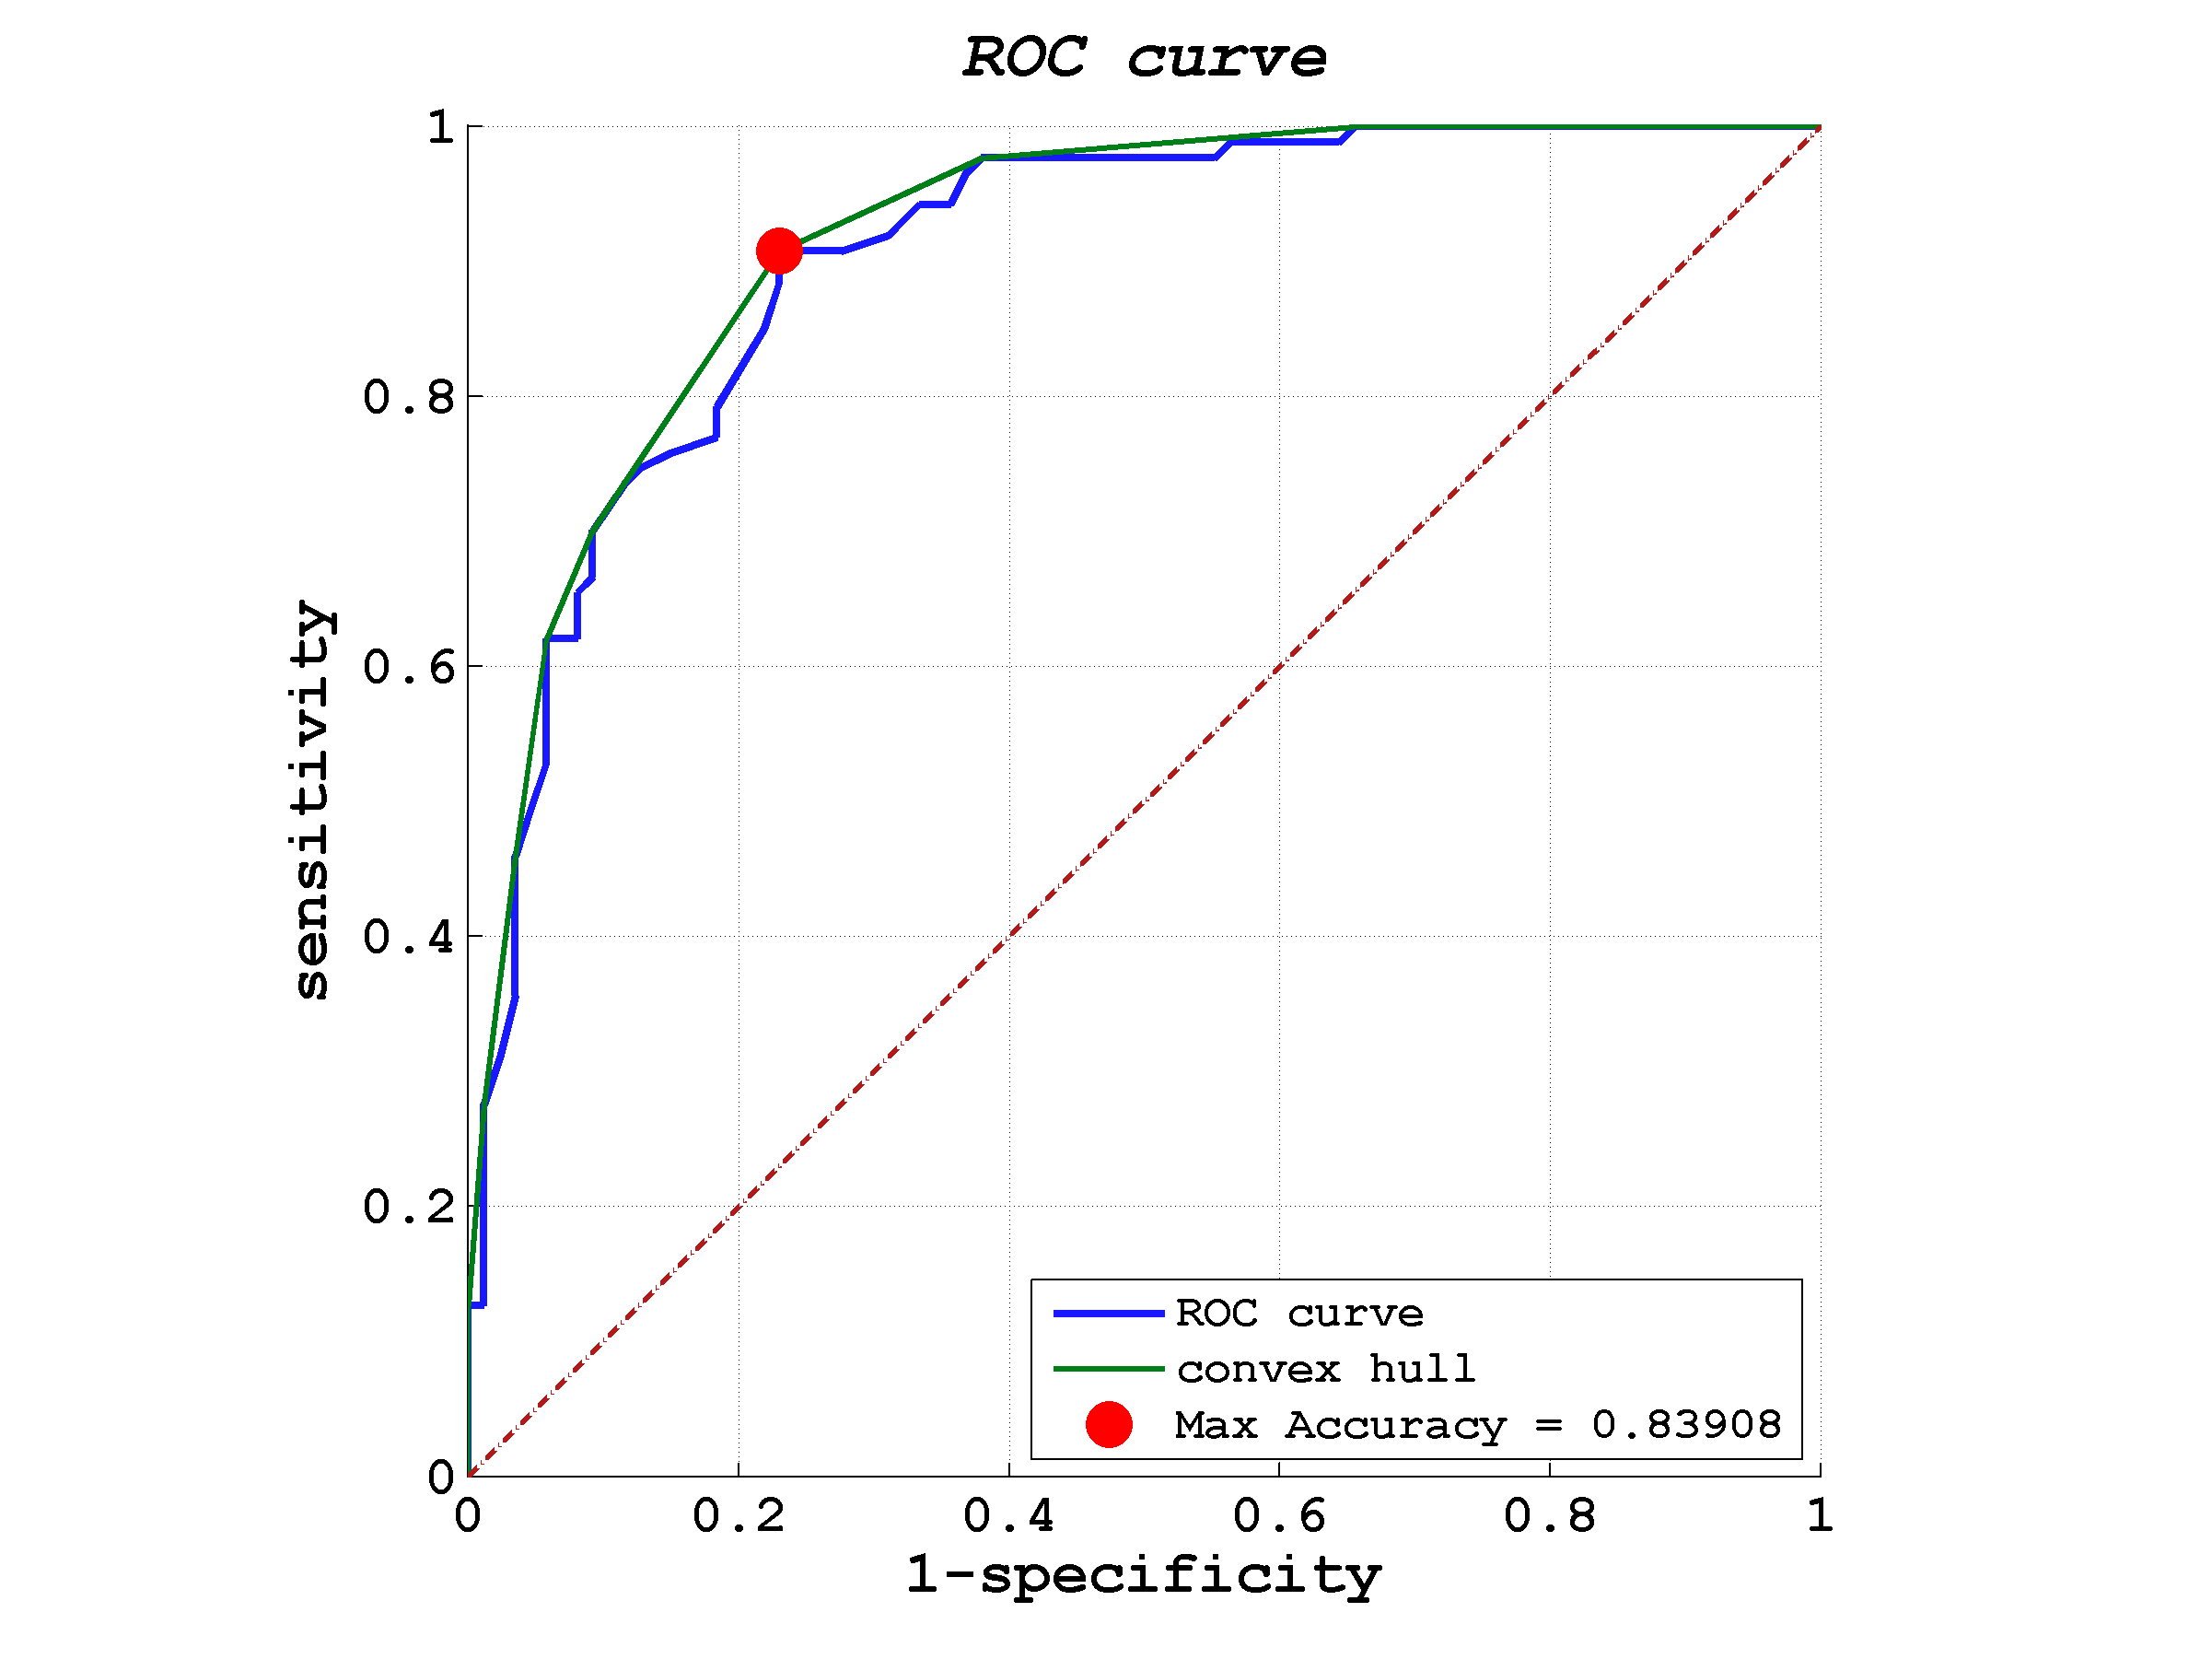
\includegraphics[width=0.46\textwidth]{./images/exp03/class/RF_iVHL_extA.png}
      \label{ch6:fig7:a}
    }
    \hspace{1mm}
    \subfigure[RF MSHL - ROC]{
      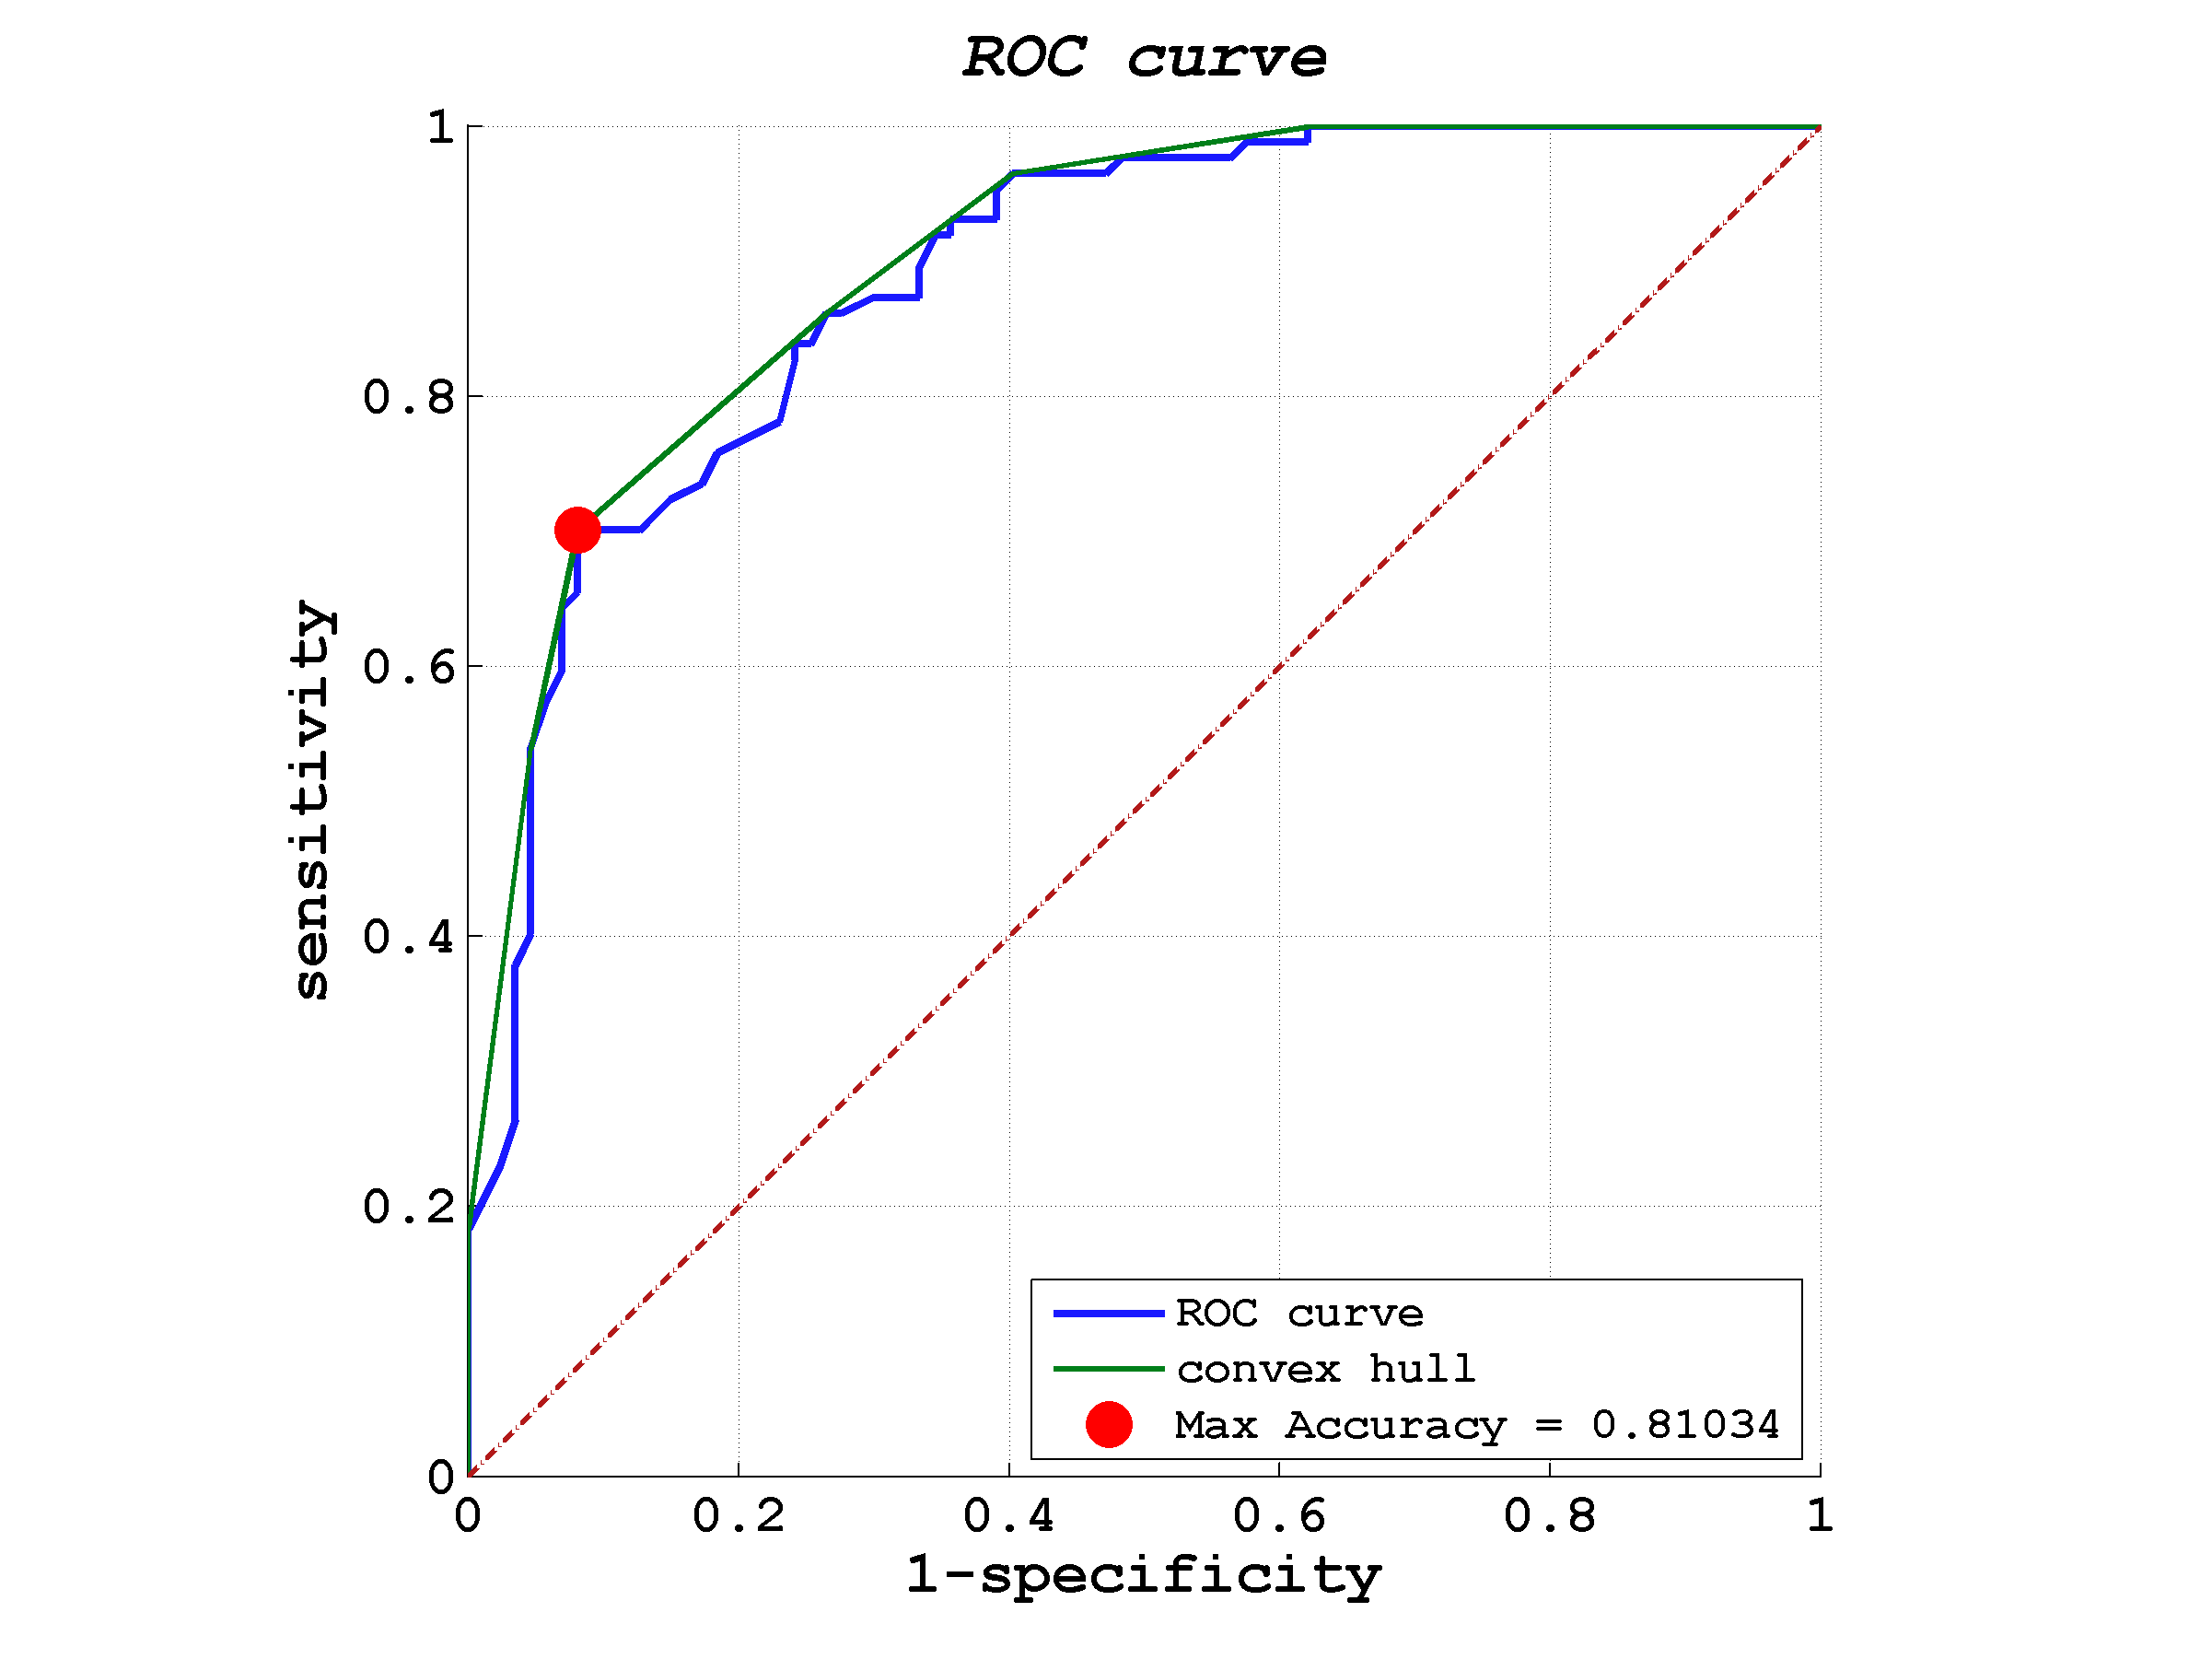
\includegraphics[width=0.46\textwidth]{./images/exp03/class/RF_MSHL_extA.png}
      \label{ch6:fig7:b}
    }
    \\
    \subfigure[RF MSiVHR - ROC]{
      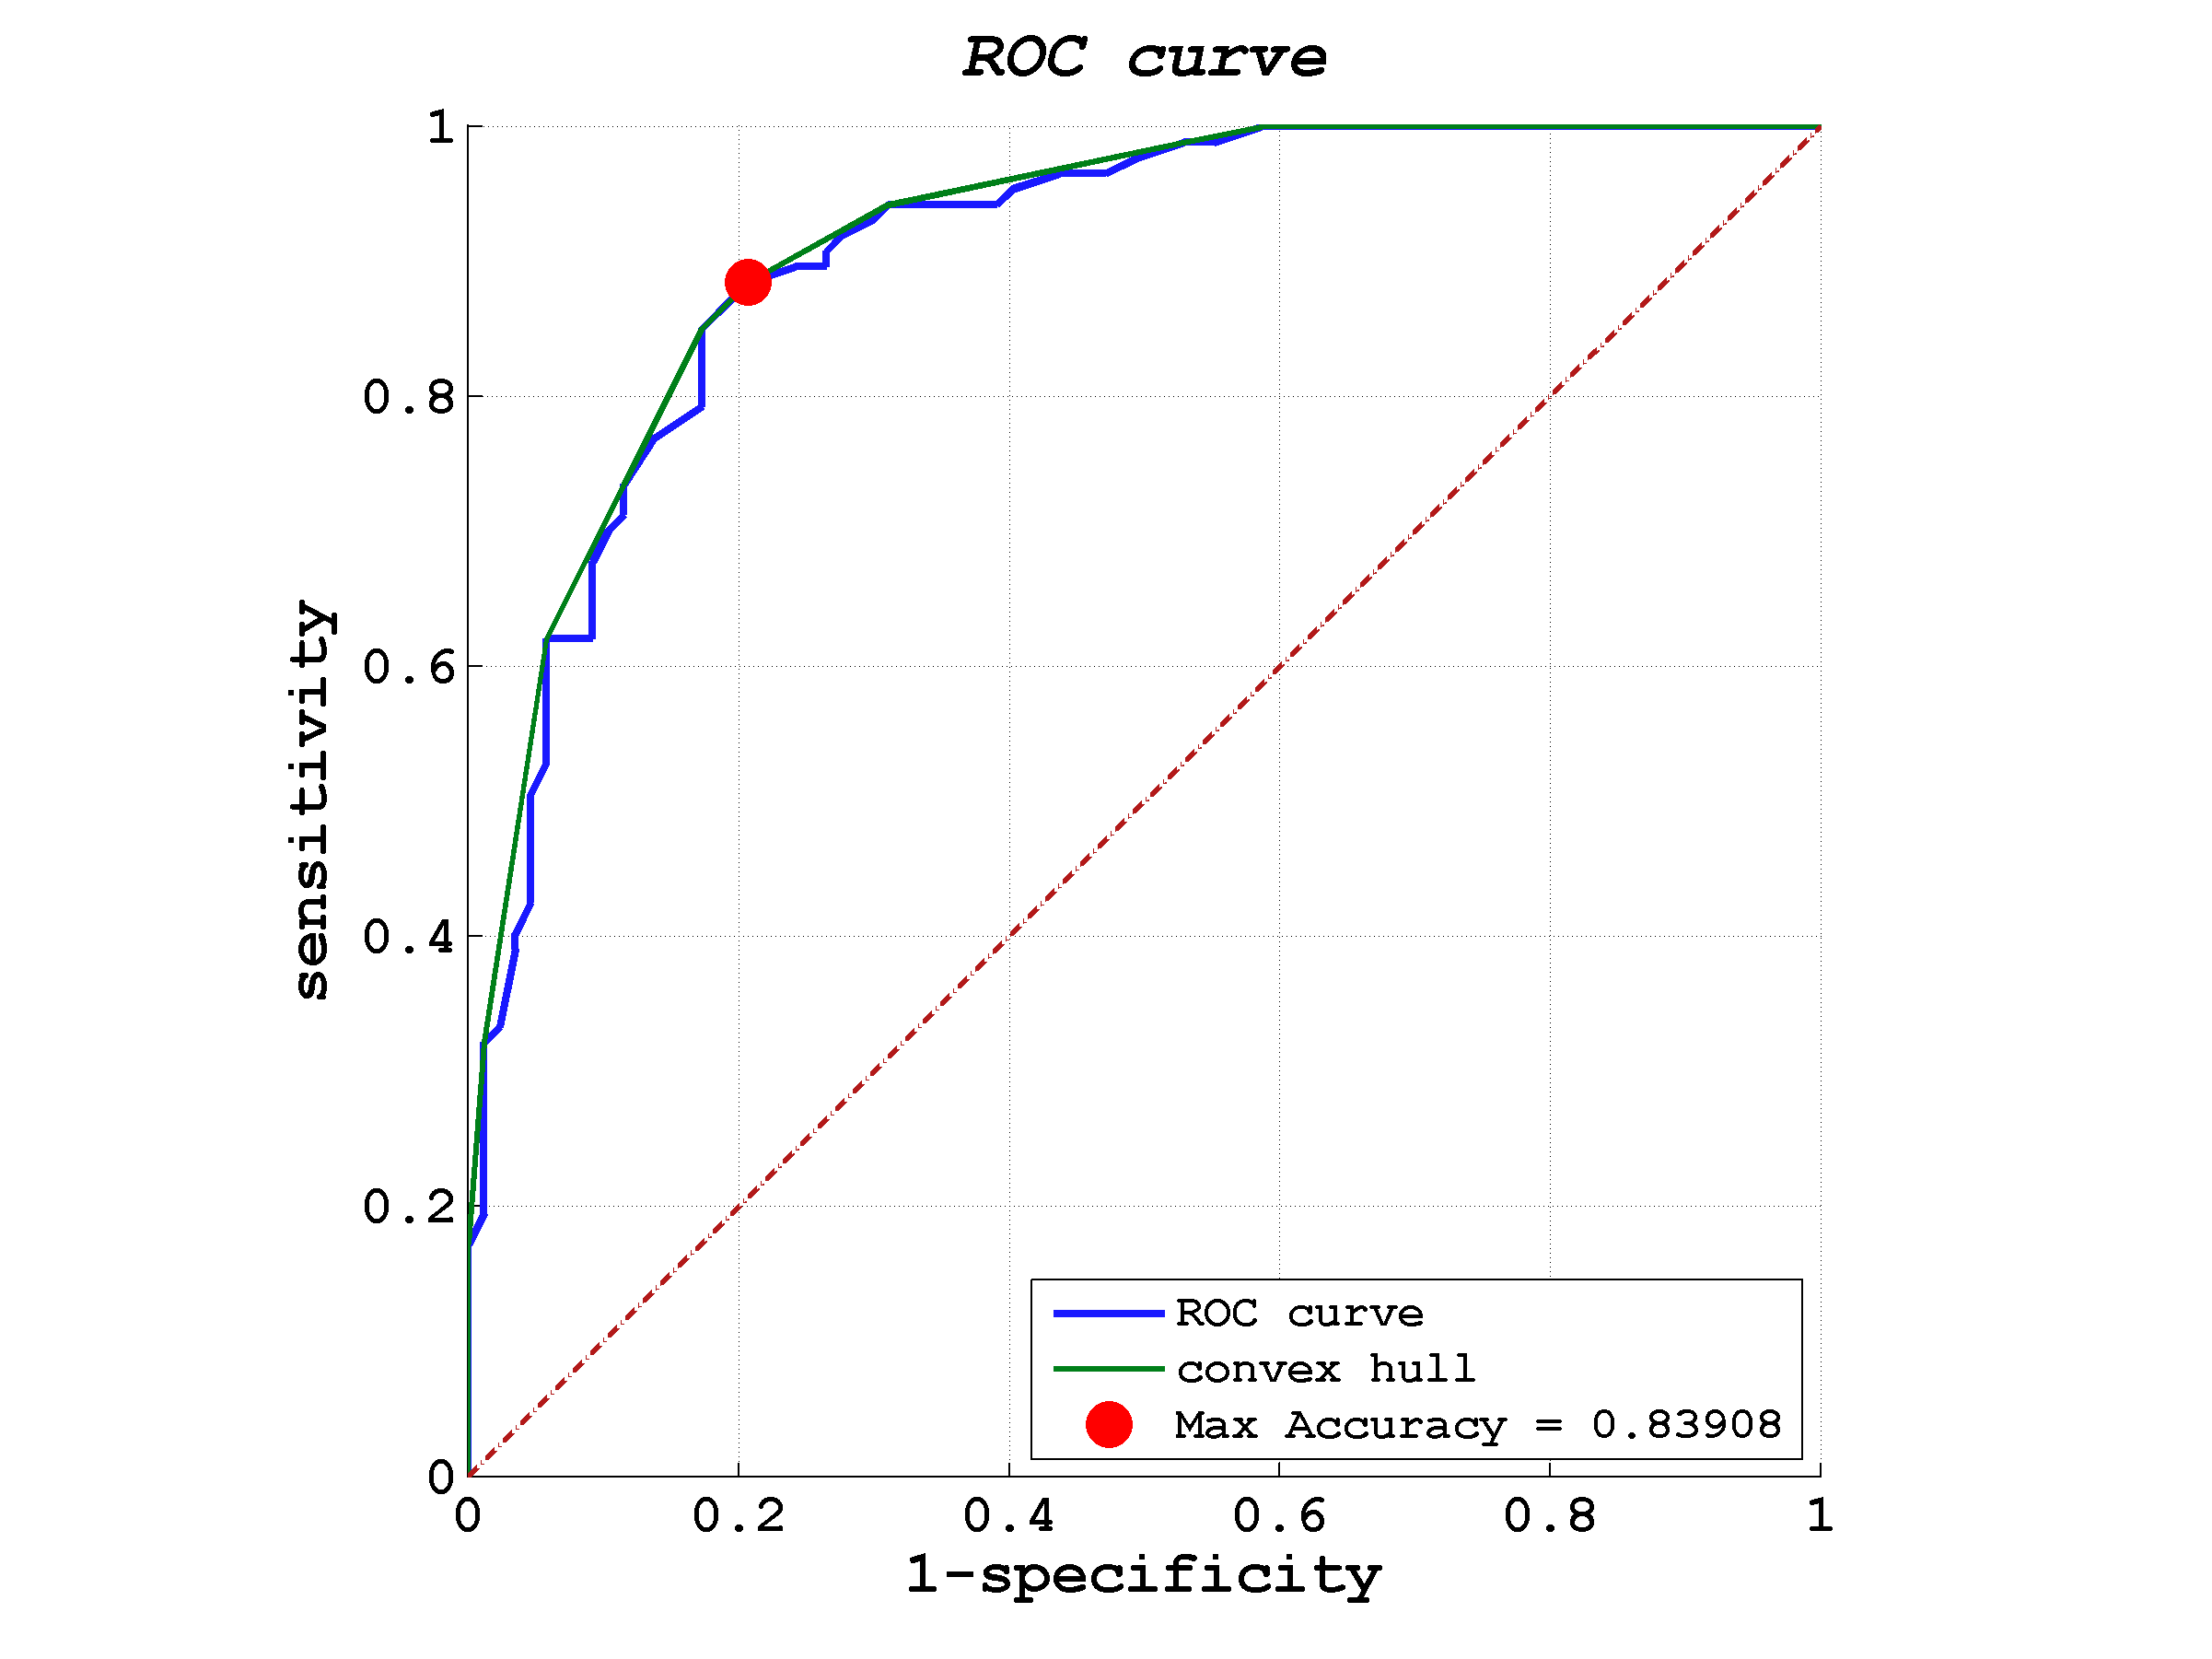
\includegraphics[width=0.46\textwidth]{./images/exp03/class/RF_MSiVHR_extA.png}
      \label{ch6:fig7:c}
    }    
    \hspace{1mm}
    \subfigure[RF SHL - ROC]{
      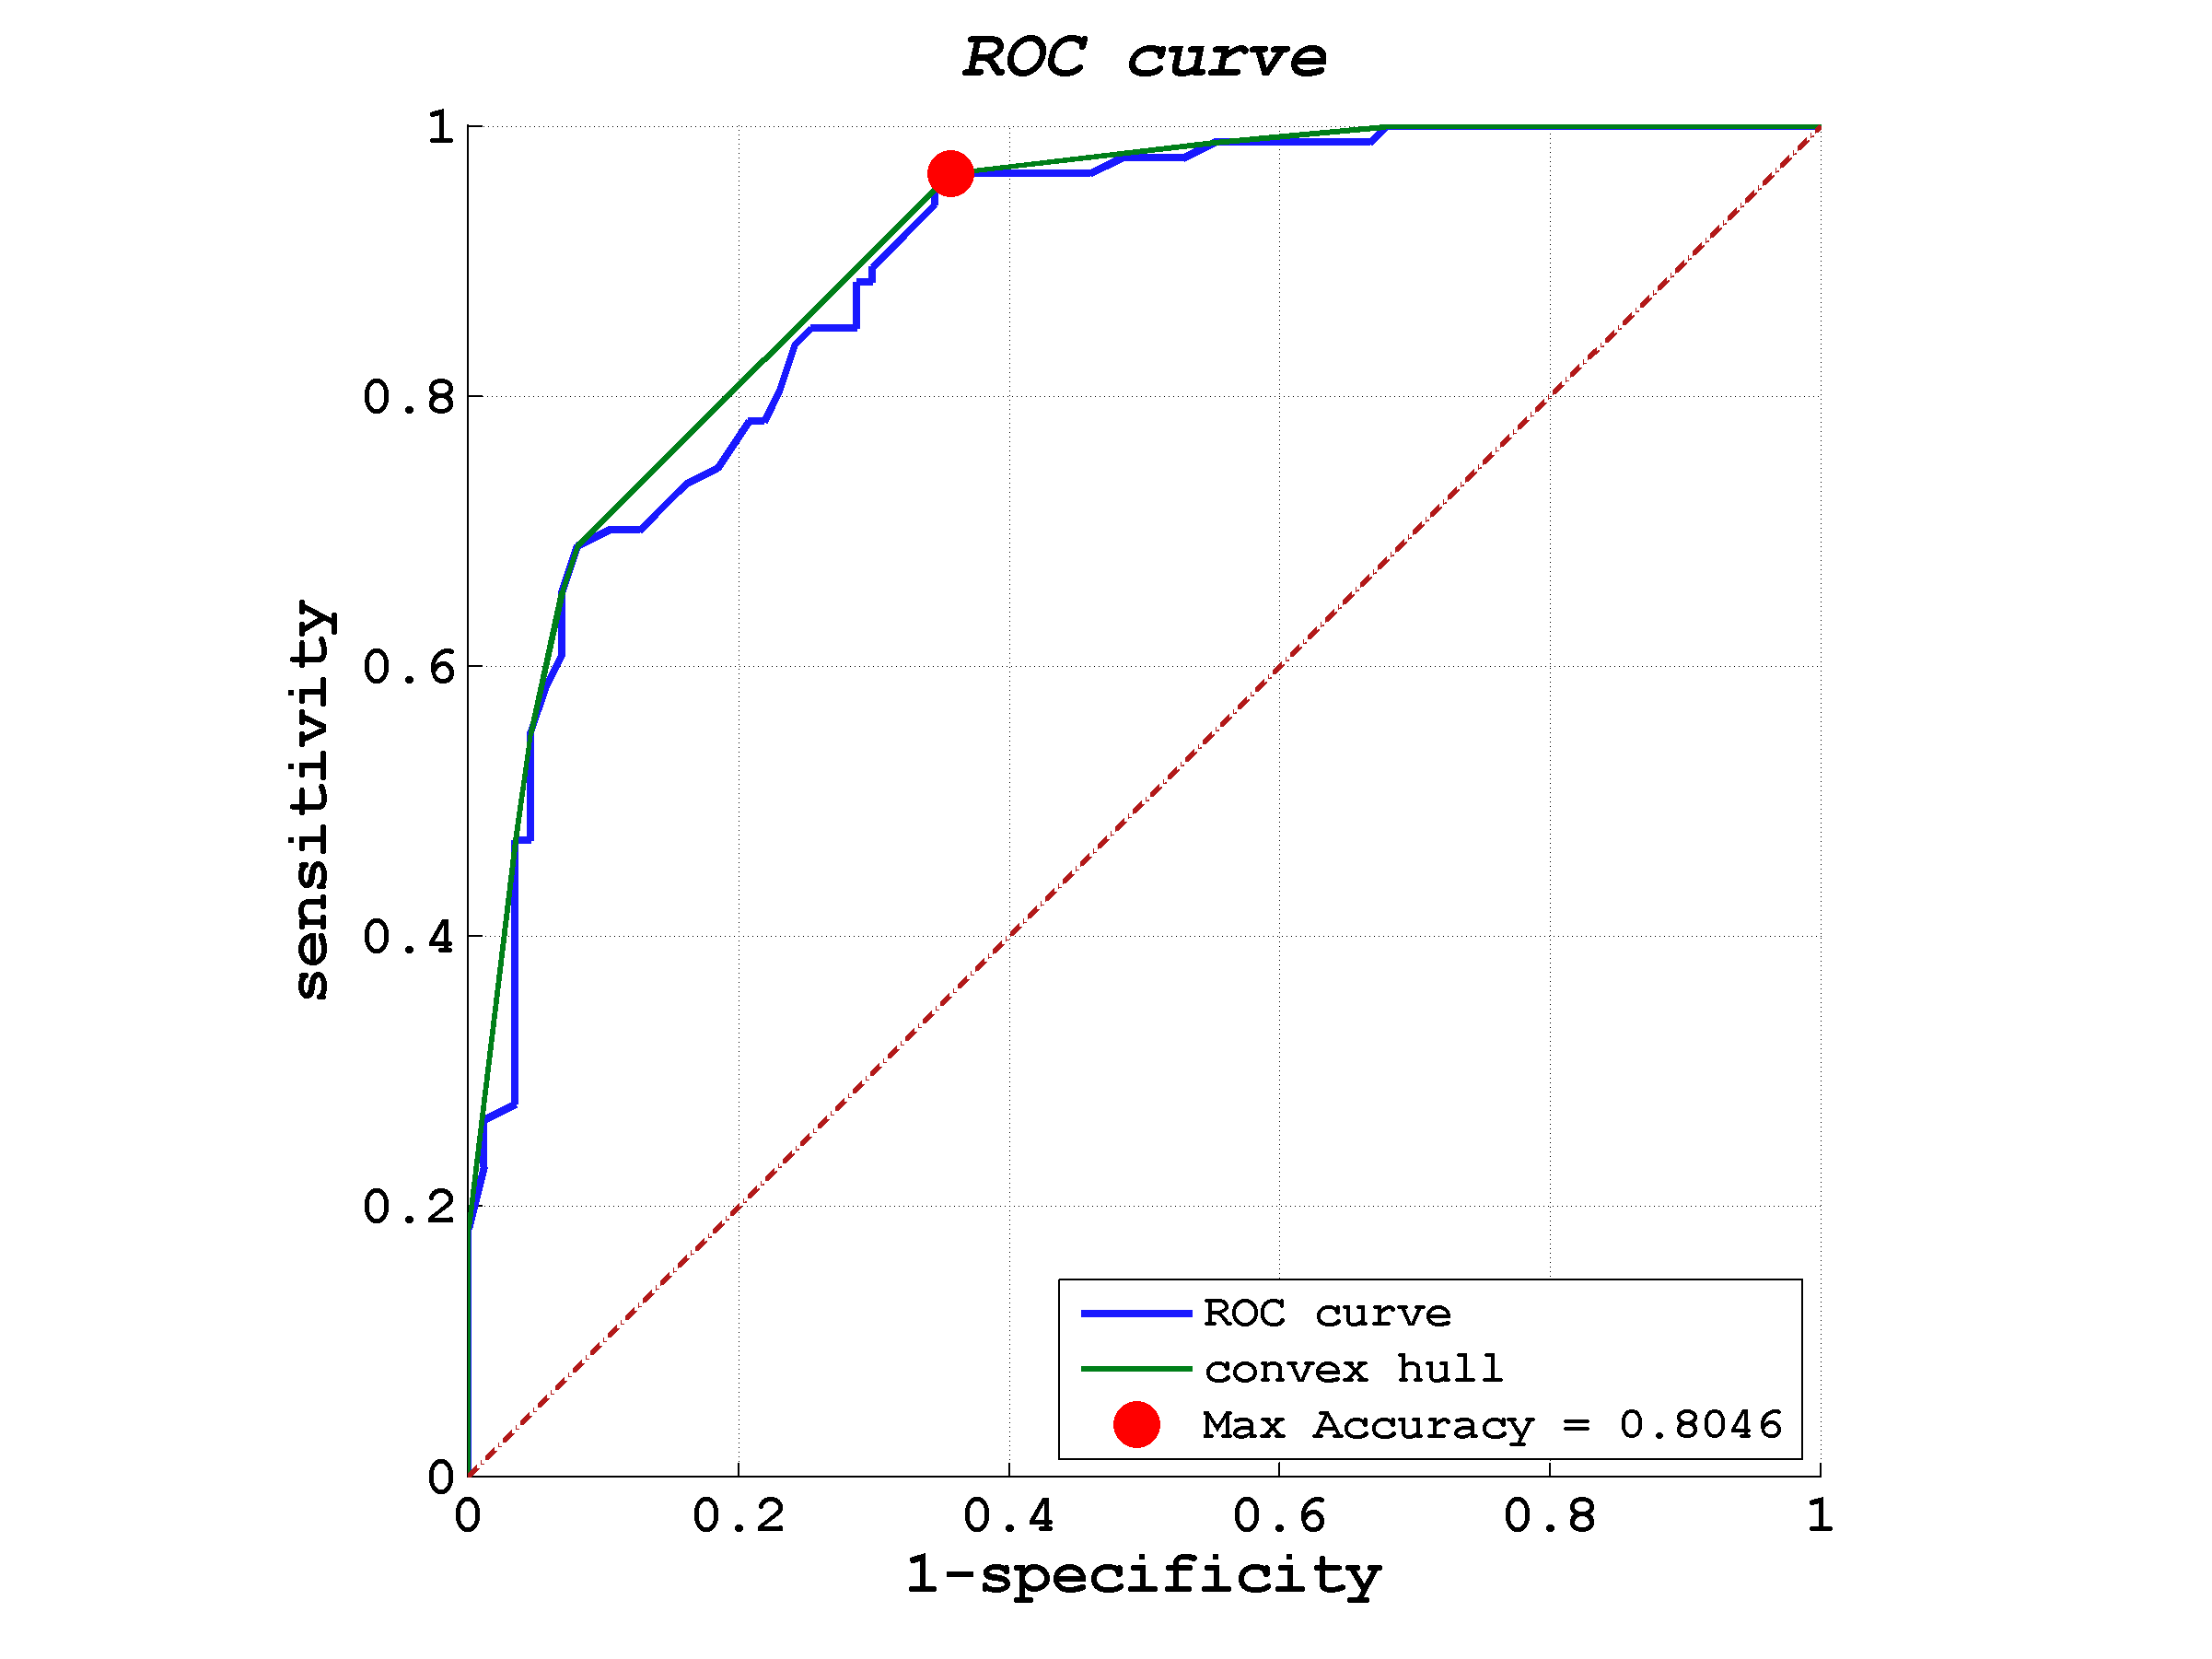
\includegraphics[width=0.46\textwidth]{./images/exp03/class/RF_SHL_extA.png}
      \label{ch6:fig7:d}
    }
    \caption{ROC curves for best feature-set - RF classification}
    \label{ch6:fig7}
\end{figure}

\vspace{0.5cm}

\subsubsection{Comparison between classifiers}

Having classified our evaluation set with a considerable number of different features, we could try to answer the question
whether one of the two considered classifiers outperforms the other. We used, as a metric for our analysis,
the \textit{AUC} and the \textit{accuracy}, and considered the three different complete feature sets: \texttt{MSiVHU}, \texttt{MSiVHR} and \texttt{MSiVHL}.
Having tried all the possible combinations, the sorted the results obtained by the \Gls{RF} classifier in ascending order and plotted the results obtained by the 
\Gls{SVM} classifier in the same sequence.\\
The results are showed on Figures \ref{ch6:fig8}, \ref{ch6:fig9} and \ref{ch6:fig10}.


\begin{figure}[!htb]
  \centering
    \subfigure[MSiVHL - AUC]{
      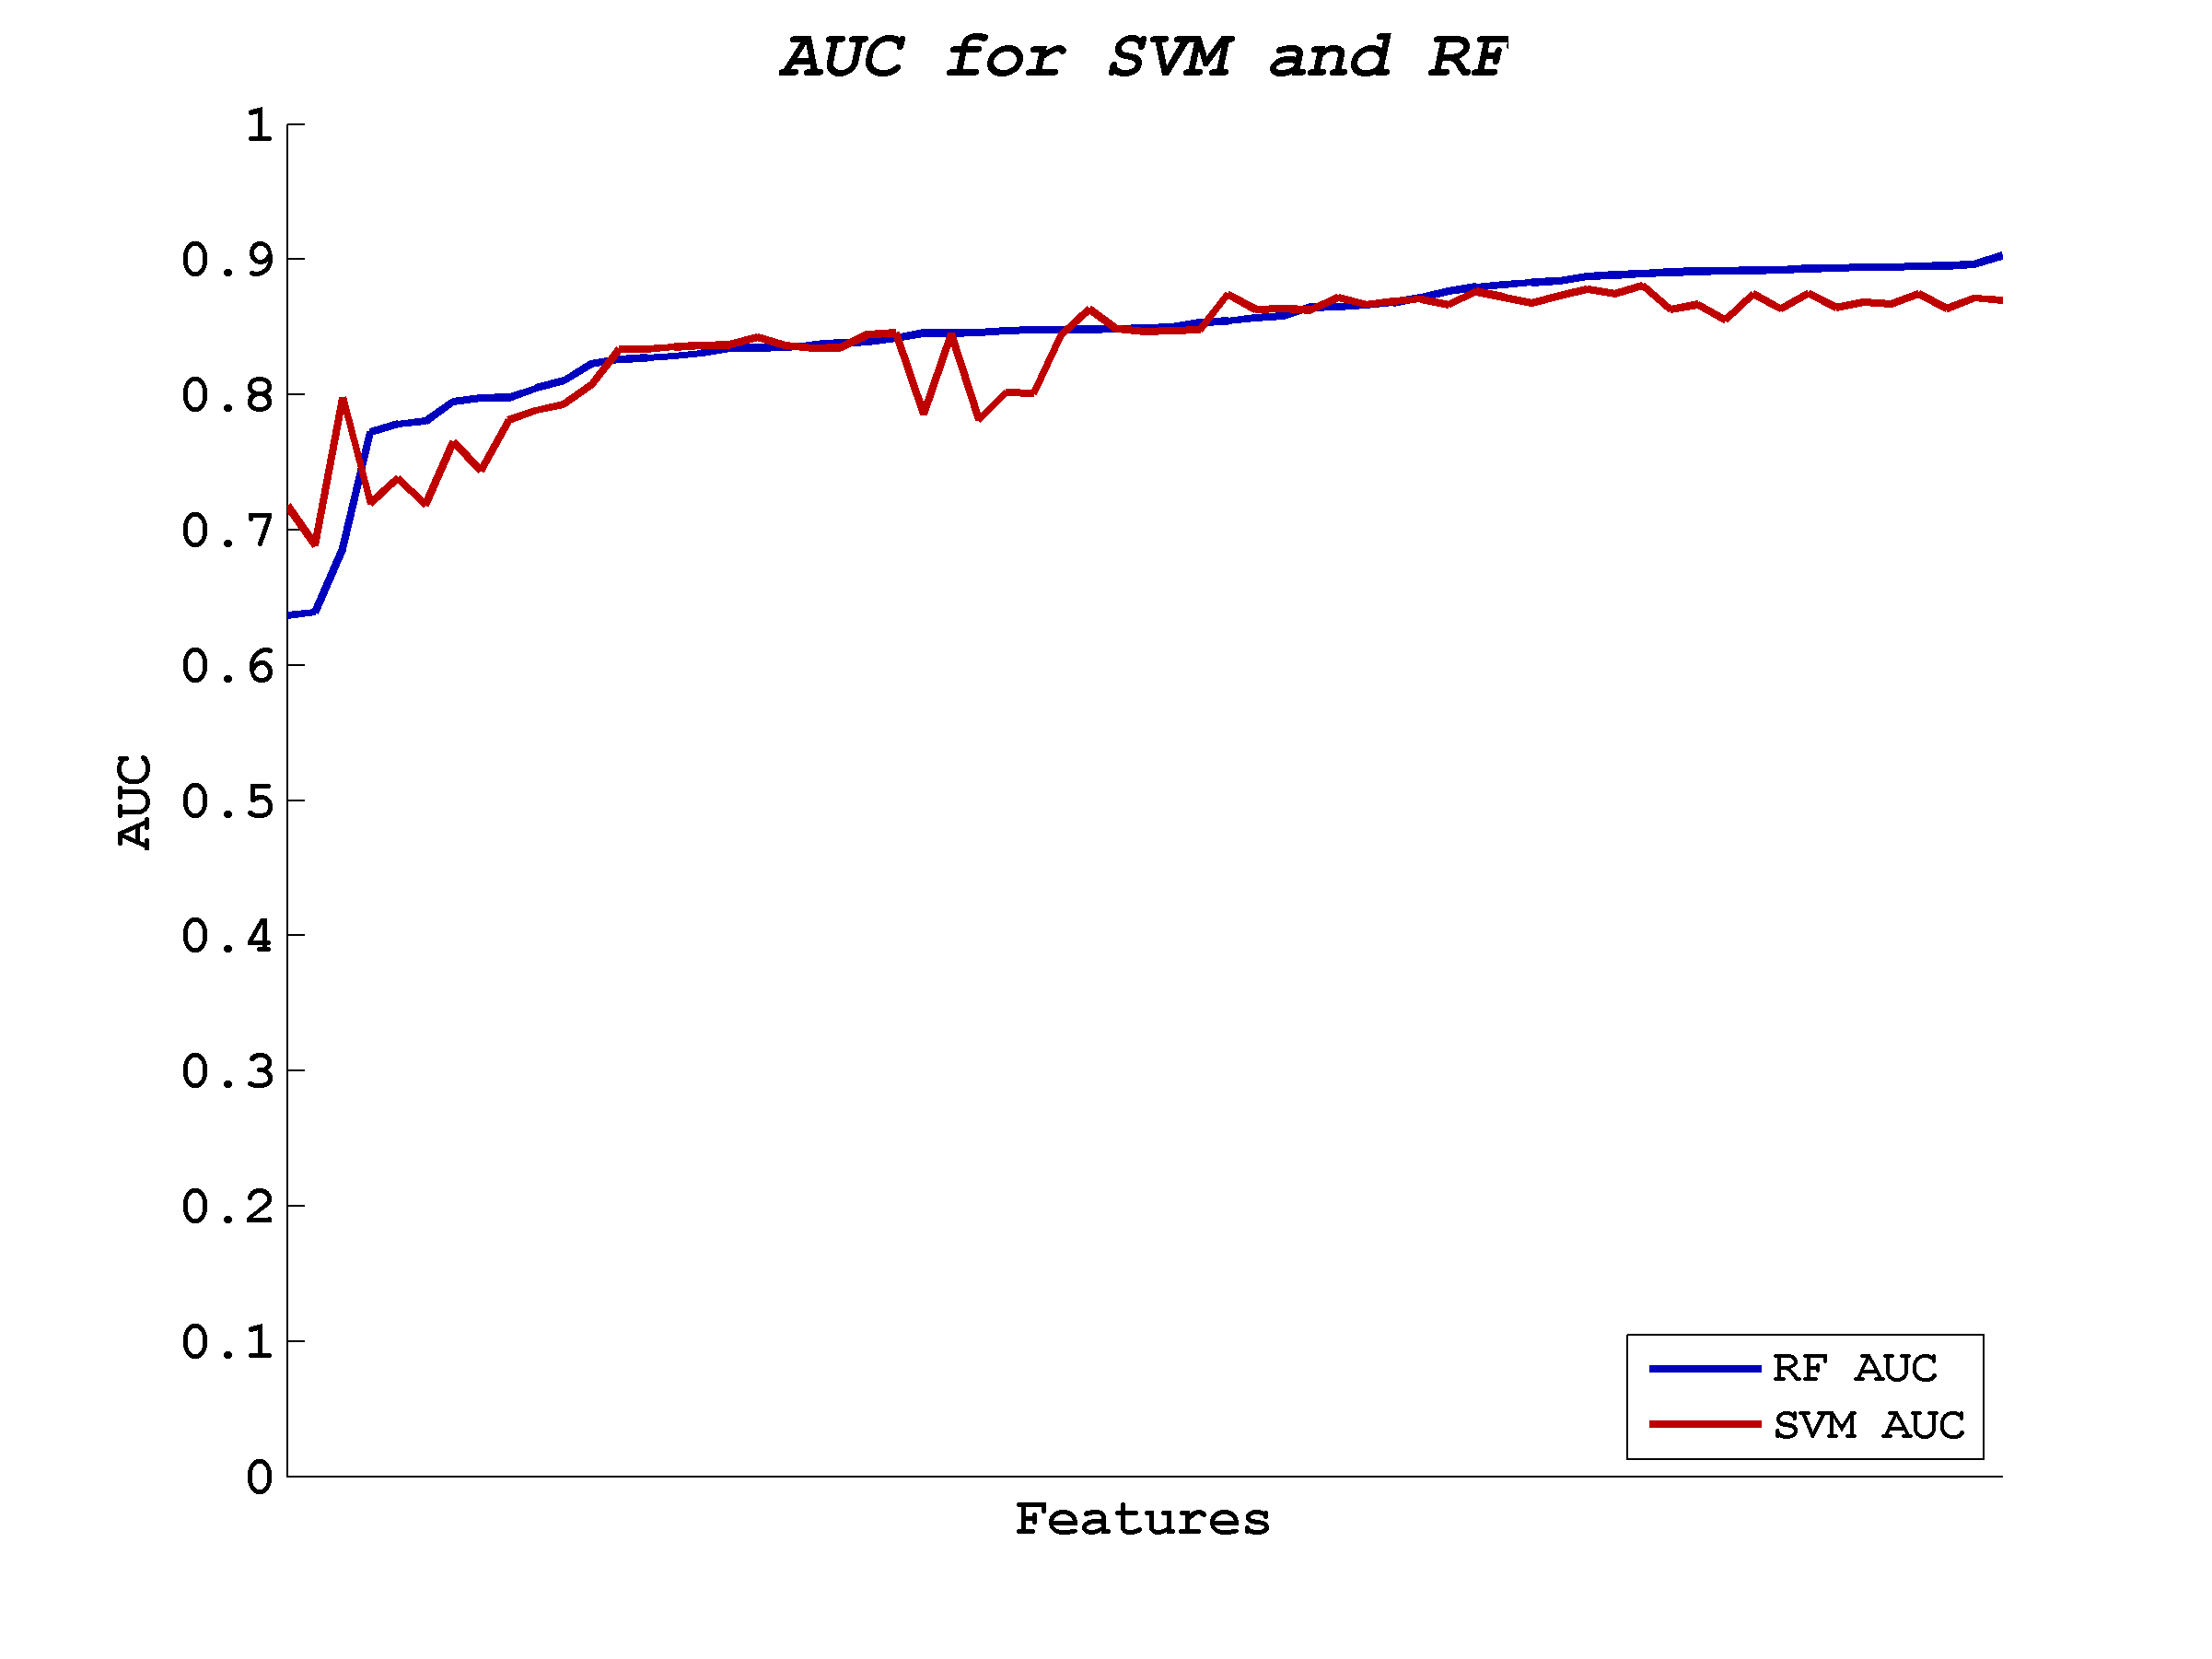
\includegraphics[width=0.46\textwidth]{./images/exp03/MSiVHL_sortAUC.png}
      \label{ch6:fig8:a}
    }
    \hspace{1mm}
    \subfigure[MSiVHL - accuracy]{
      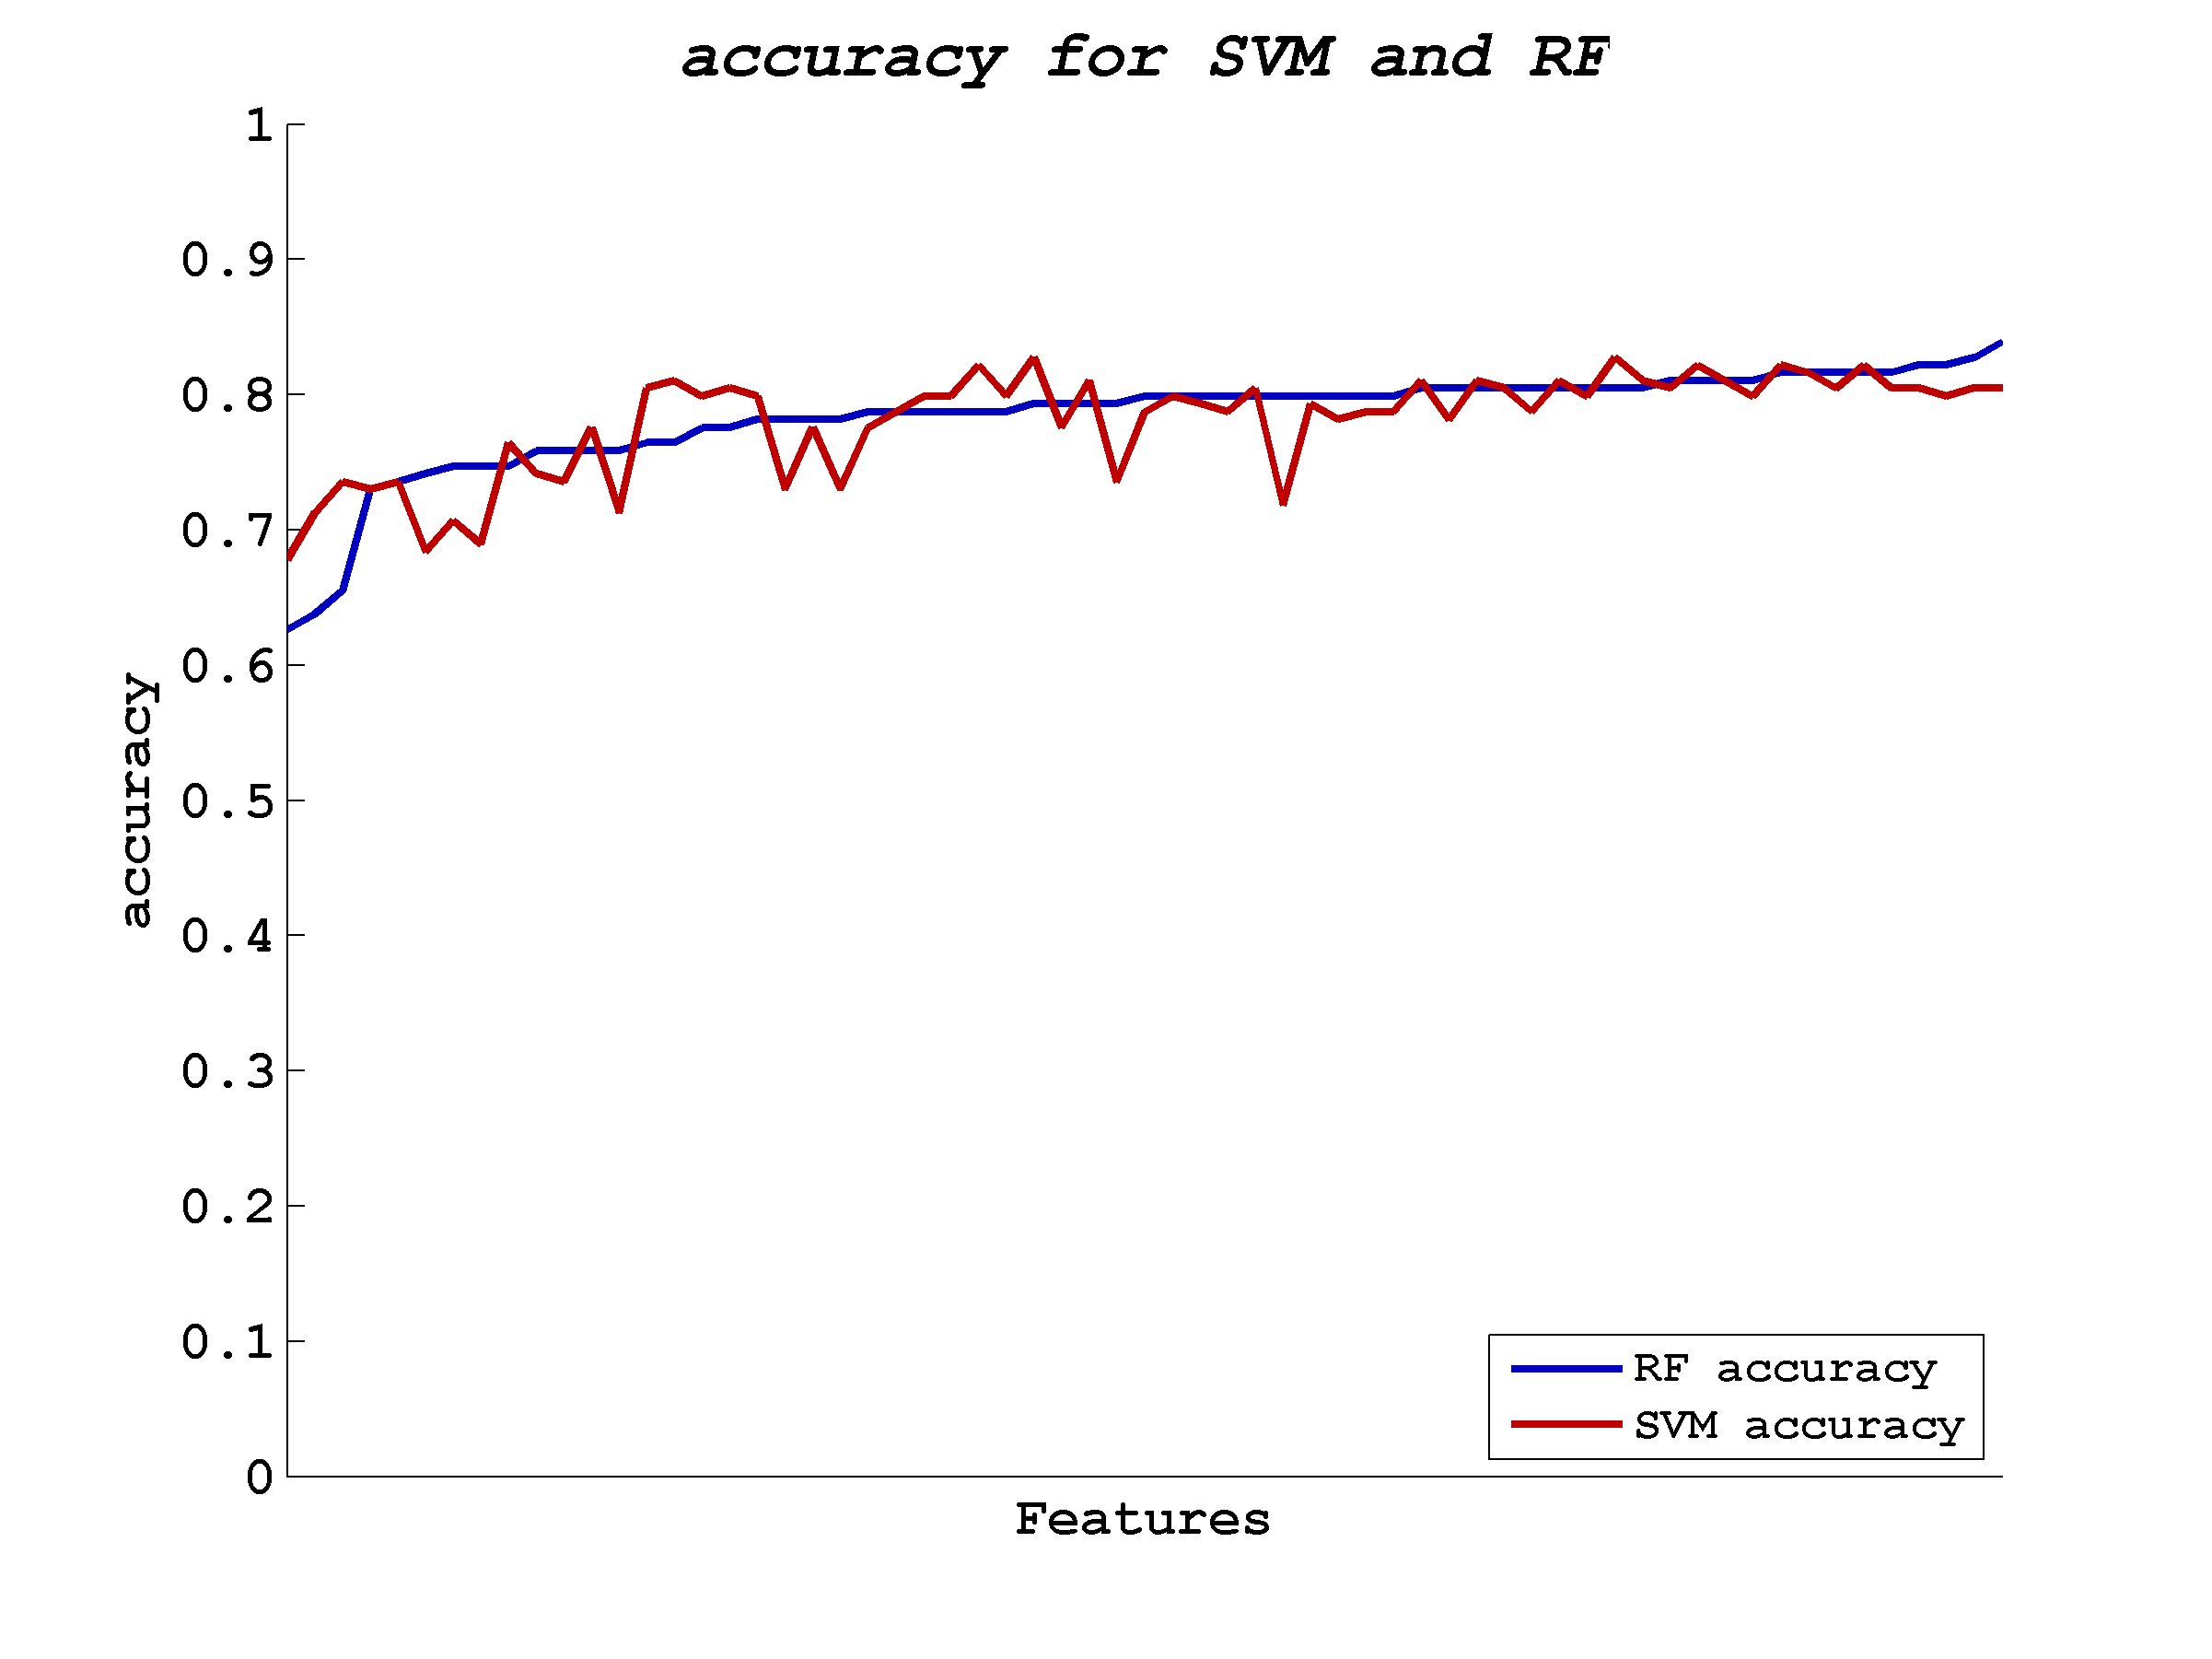
\includegraphics[width=0.46\textwidth]{./images/exp03/MSiVHL_sortAccuracy.png}
      \label{ch6:fig8:b}
    }    
    \caption{Features MSiVHL - overall performances}
    \label{ch6:fig8}
\end{figure}

\begin{figure}[!htb]
  \centering
    \subfigure[MSiVHR - AUC]{
      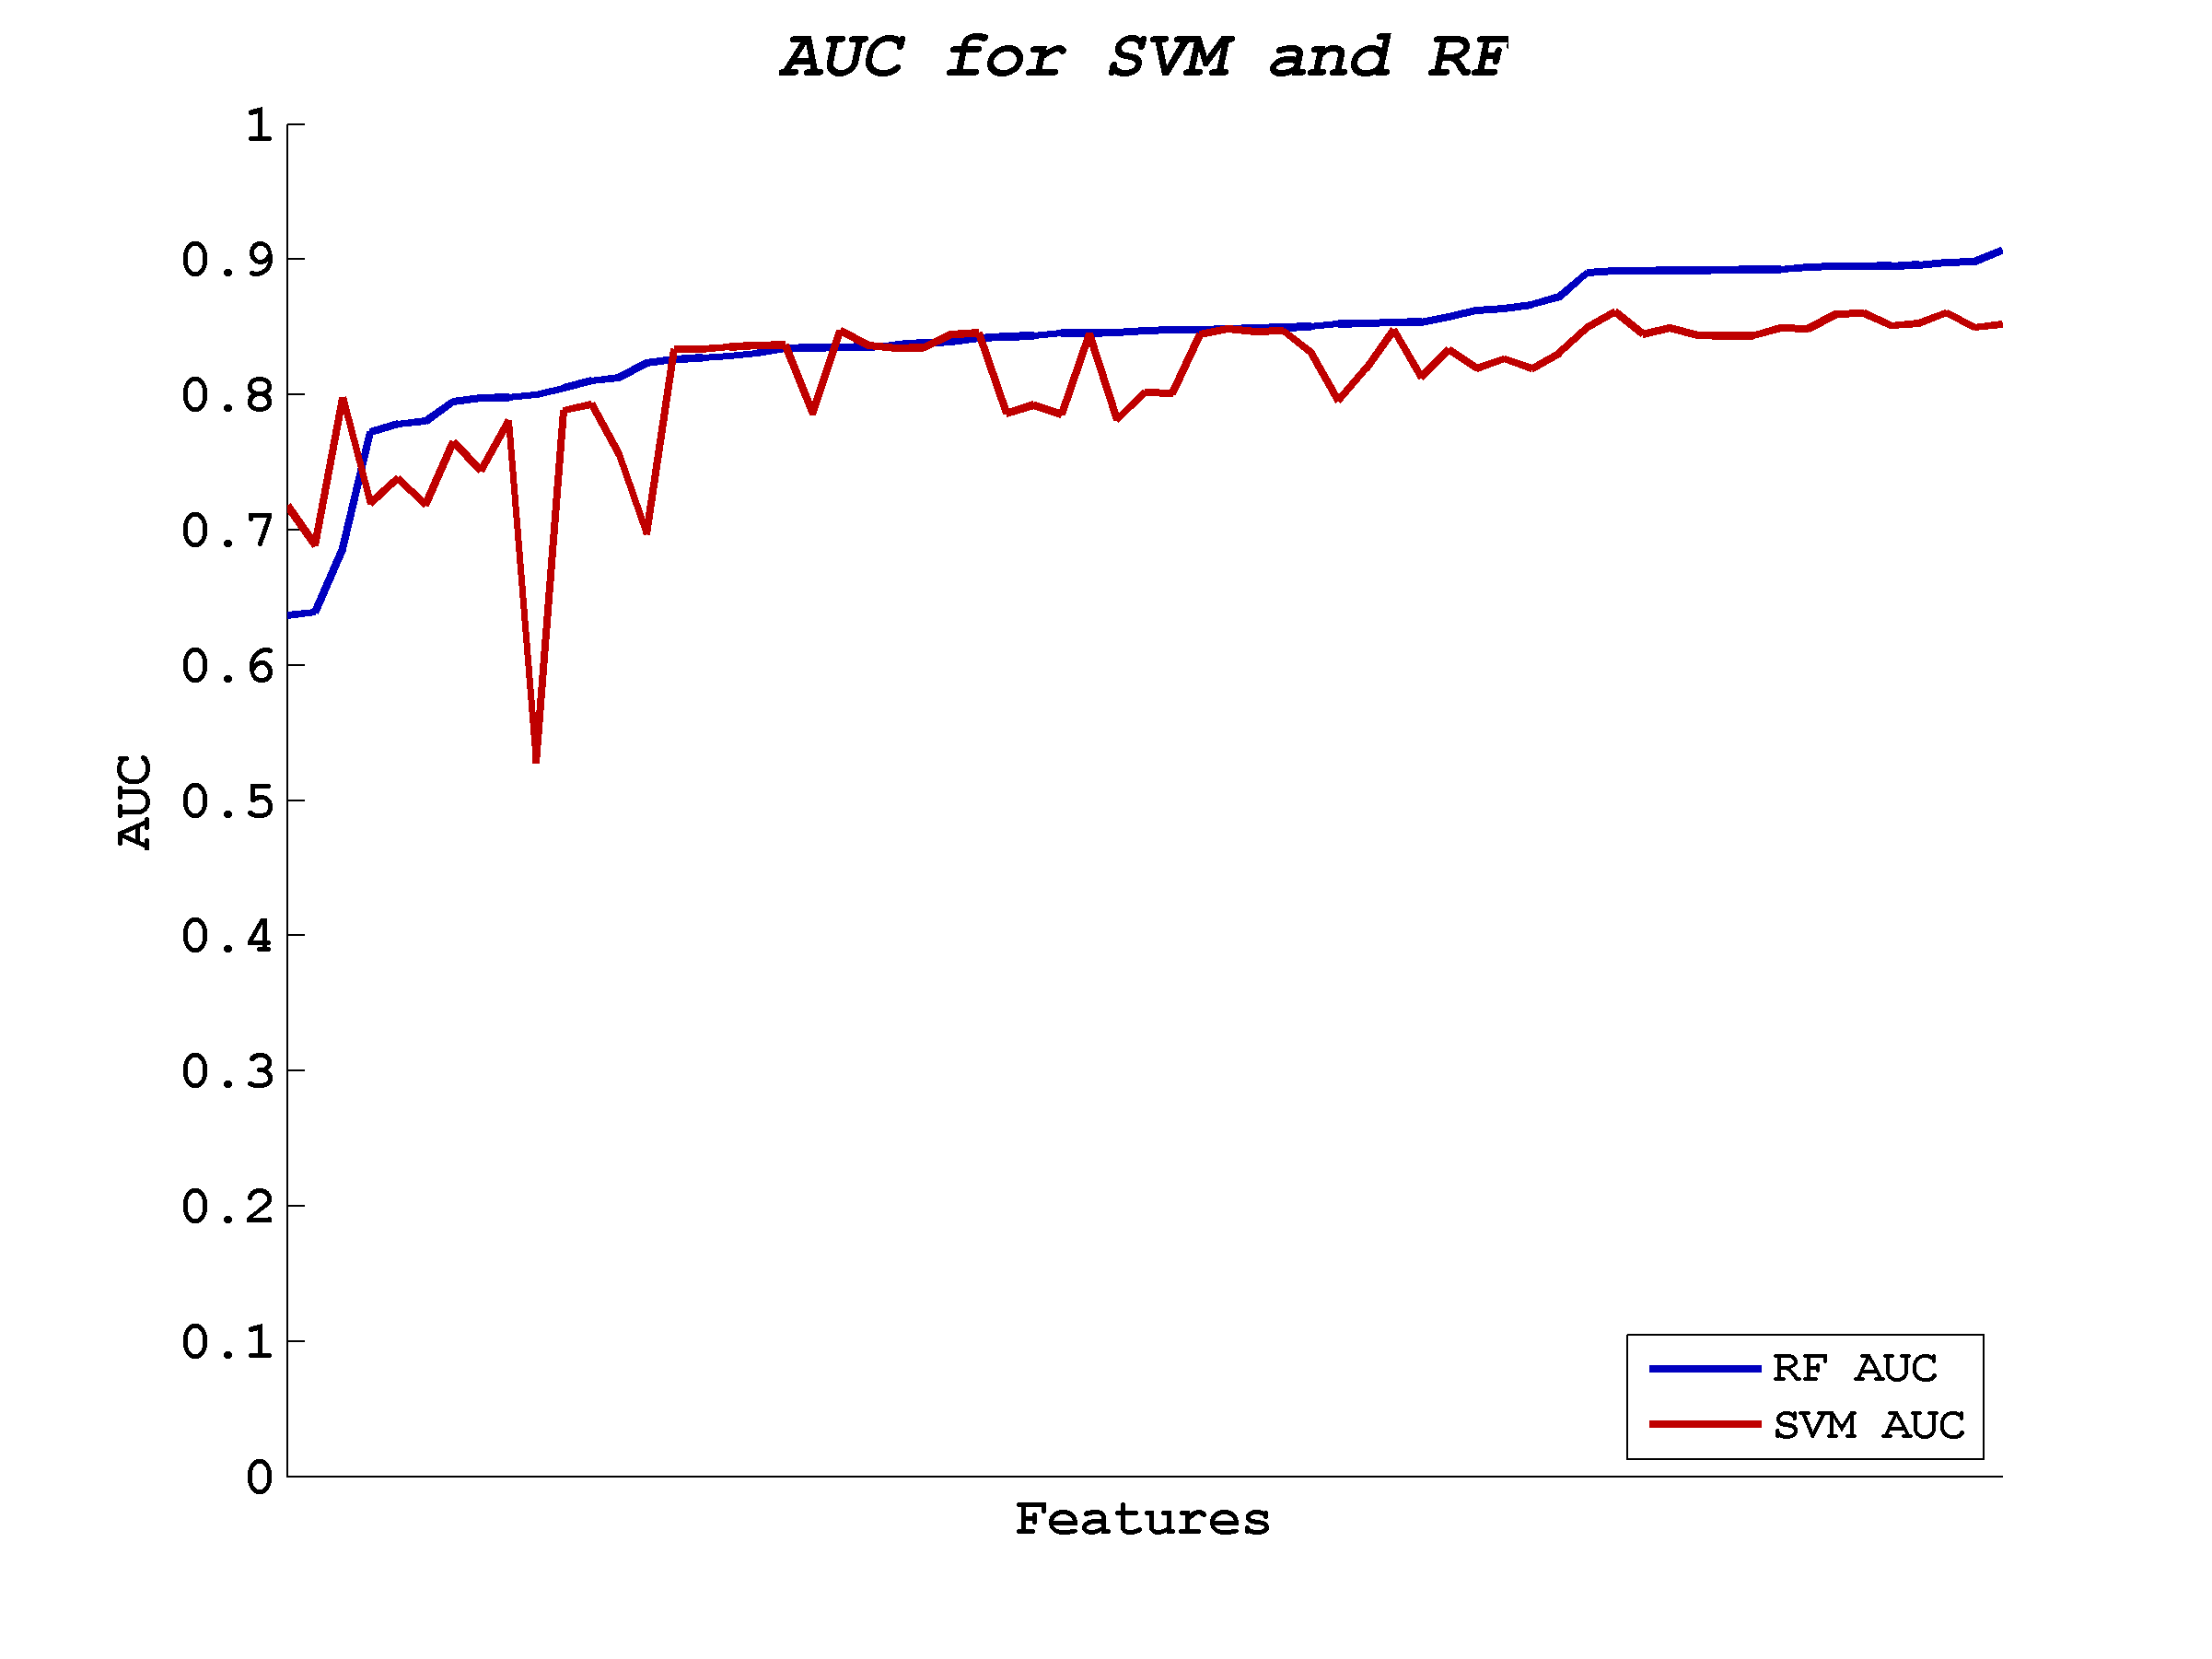
\includegraphics[width=0.46\textwidth]{./images/exp03/MSiVHR_sortAUC.png}
      \label{ch6:fig9:a}
    }
    \hspace{1mm}
    \subfigure[MSiVHR - accuracy]{
      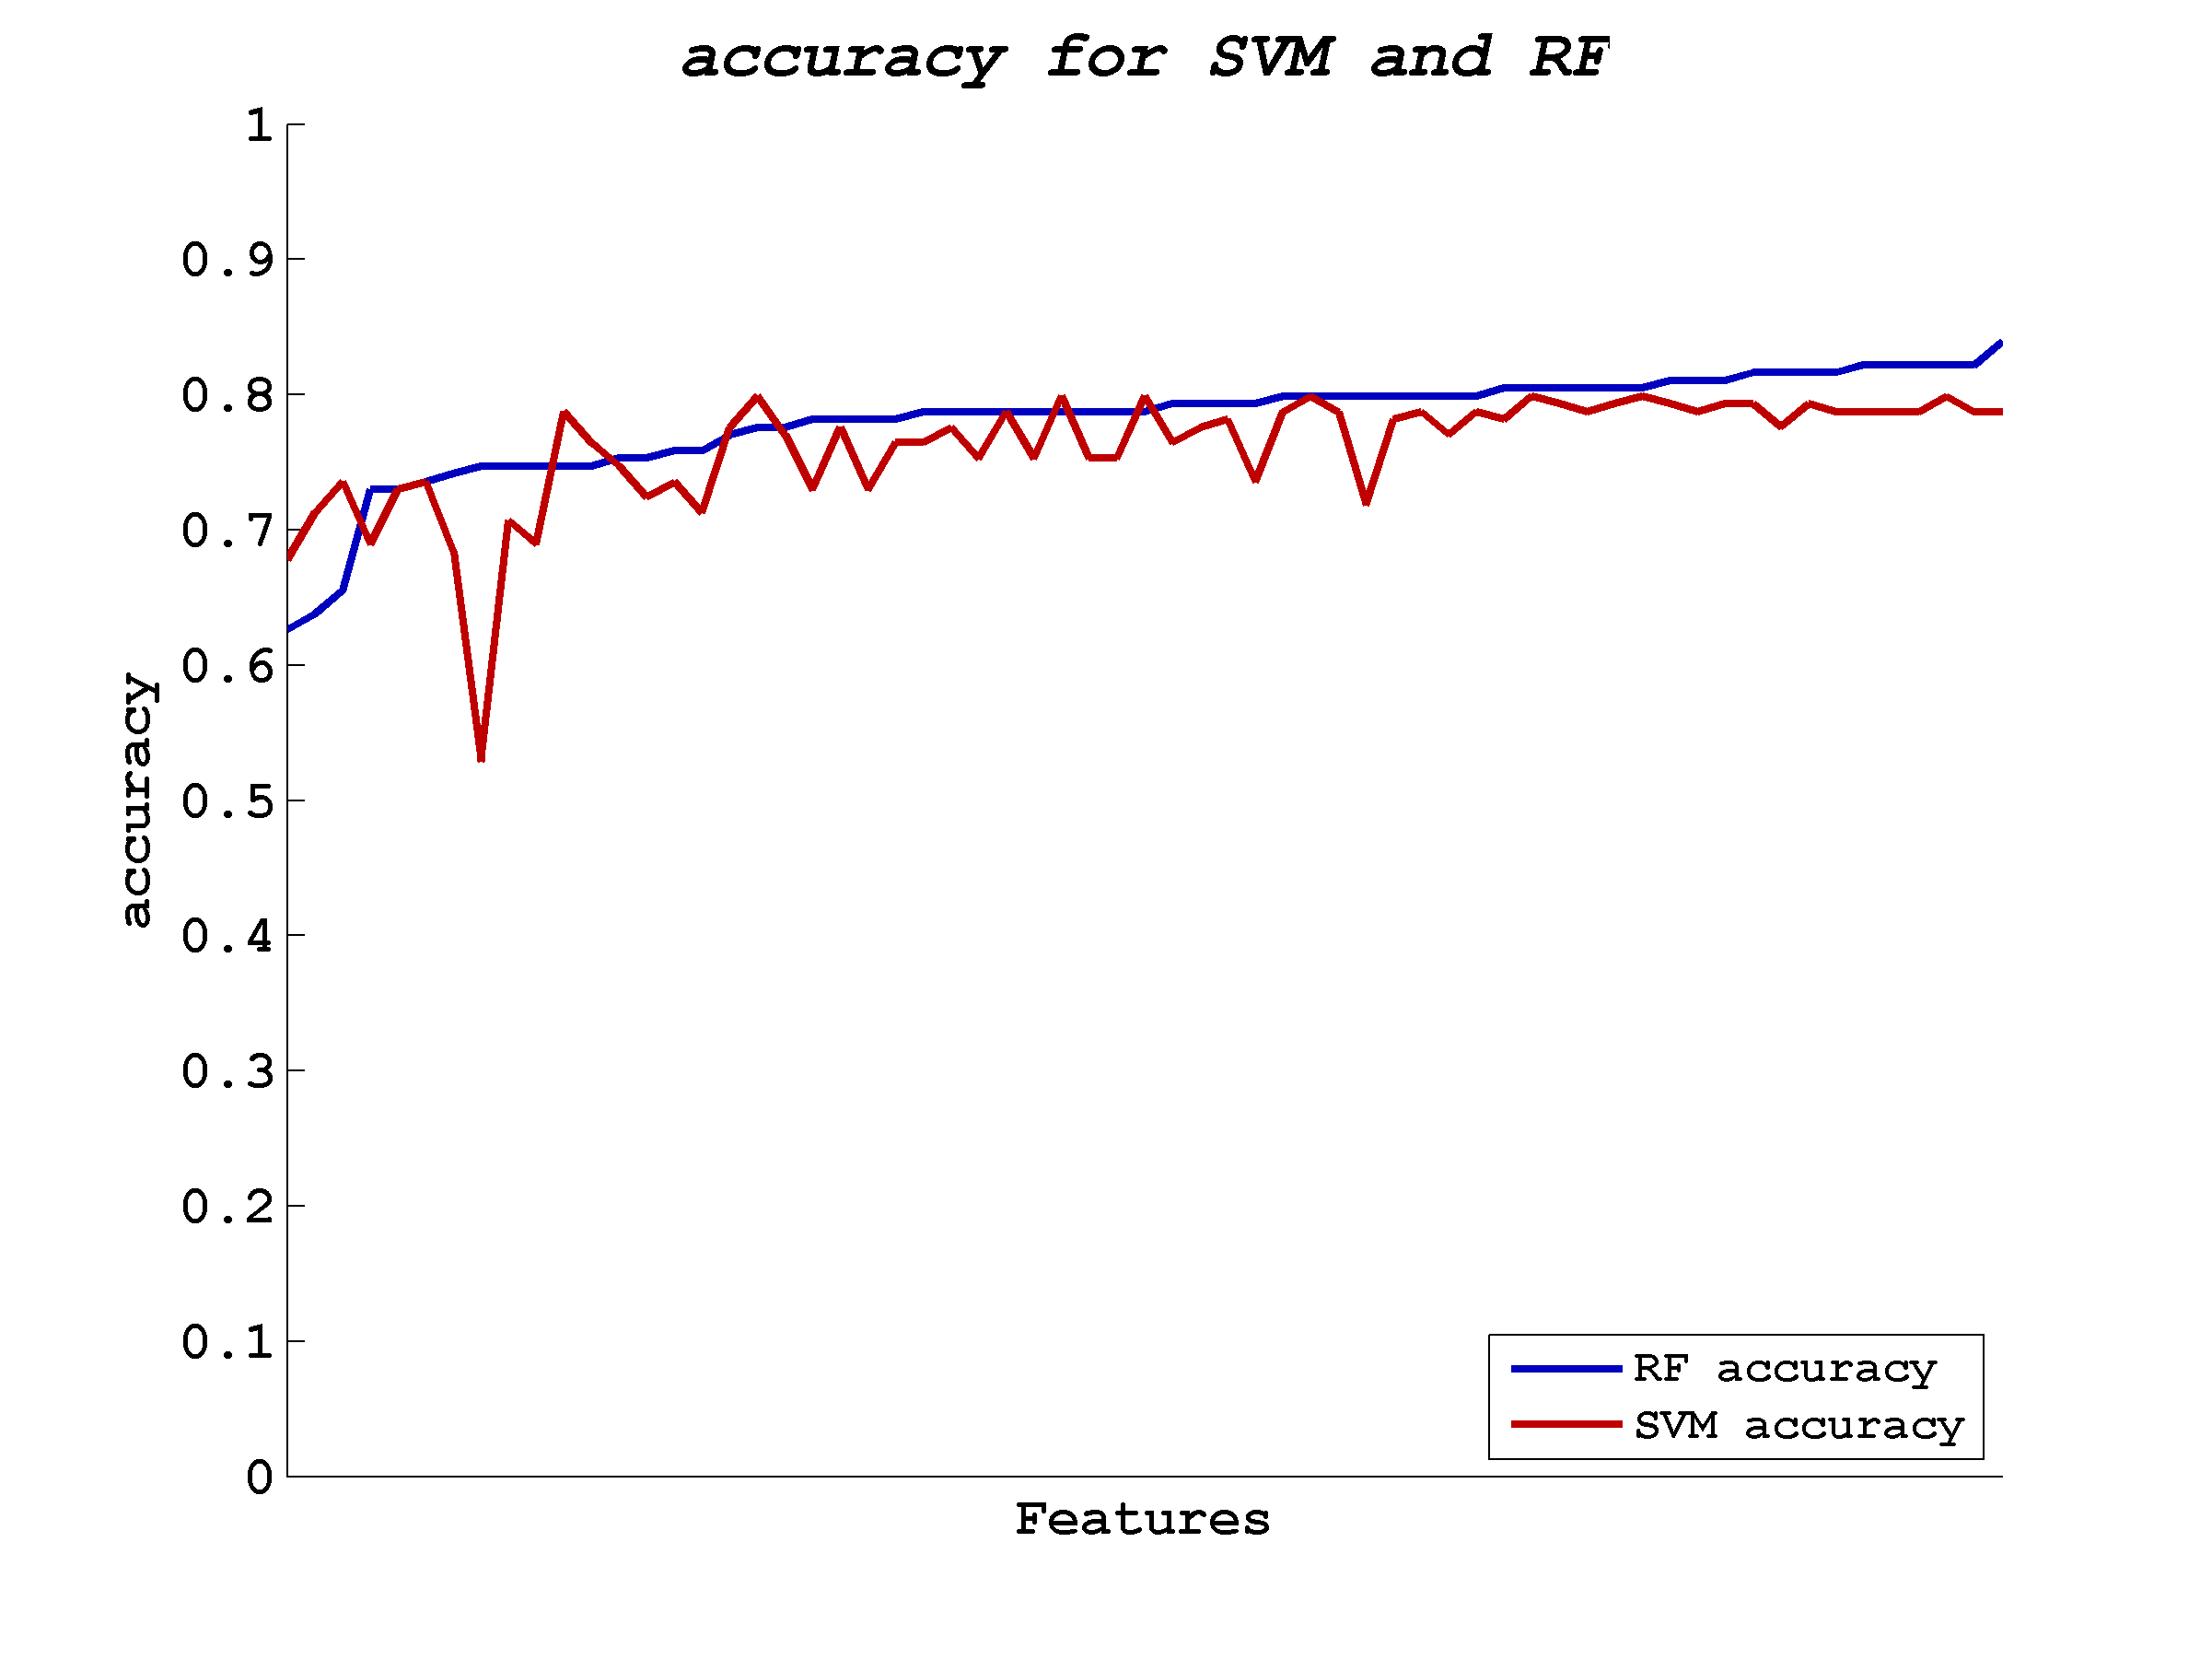
\includegraphics[width=0.46\textwidth]{./images/exp03/MSiVHR_sortAccuracy.png}
      \label{ch6:fig9:b}
    }    
    \caption{Features MSiVHR - overall performances}
    \label{ch6:fig9}
\end{figure}

\begin{figure}[!htb]
  \centering
    \subfigure[MSiVHU - AUC]{
      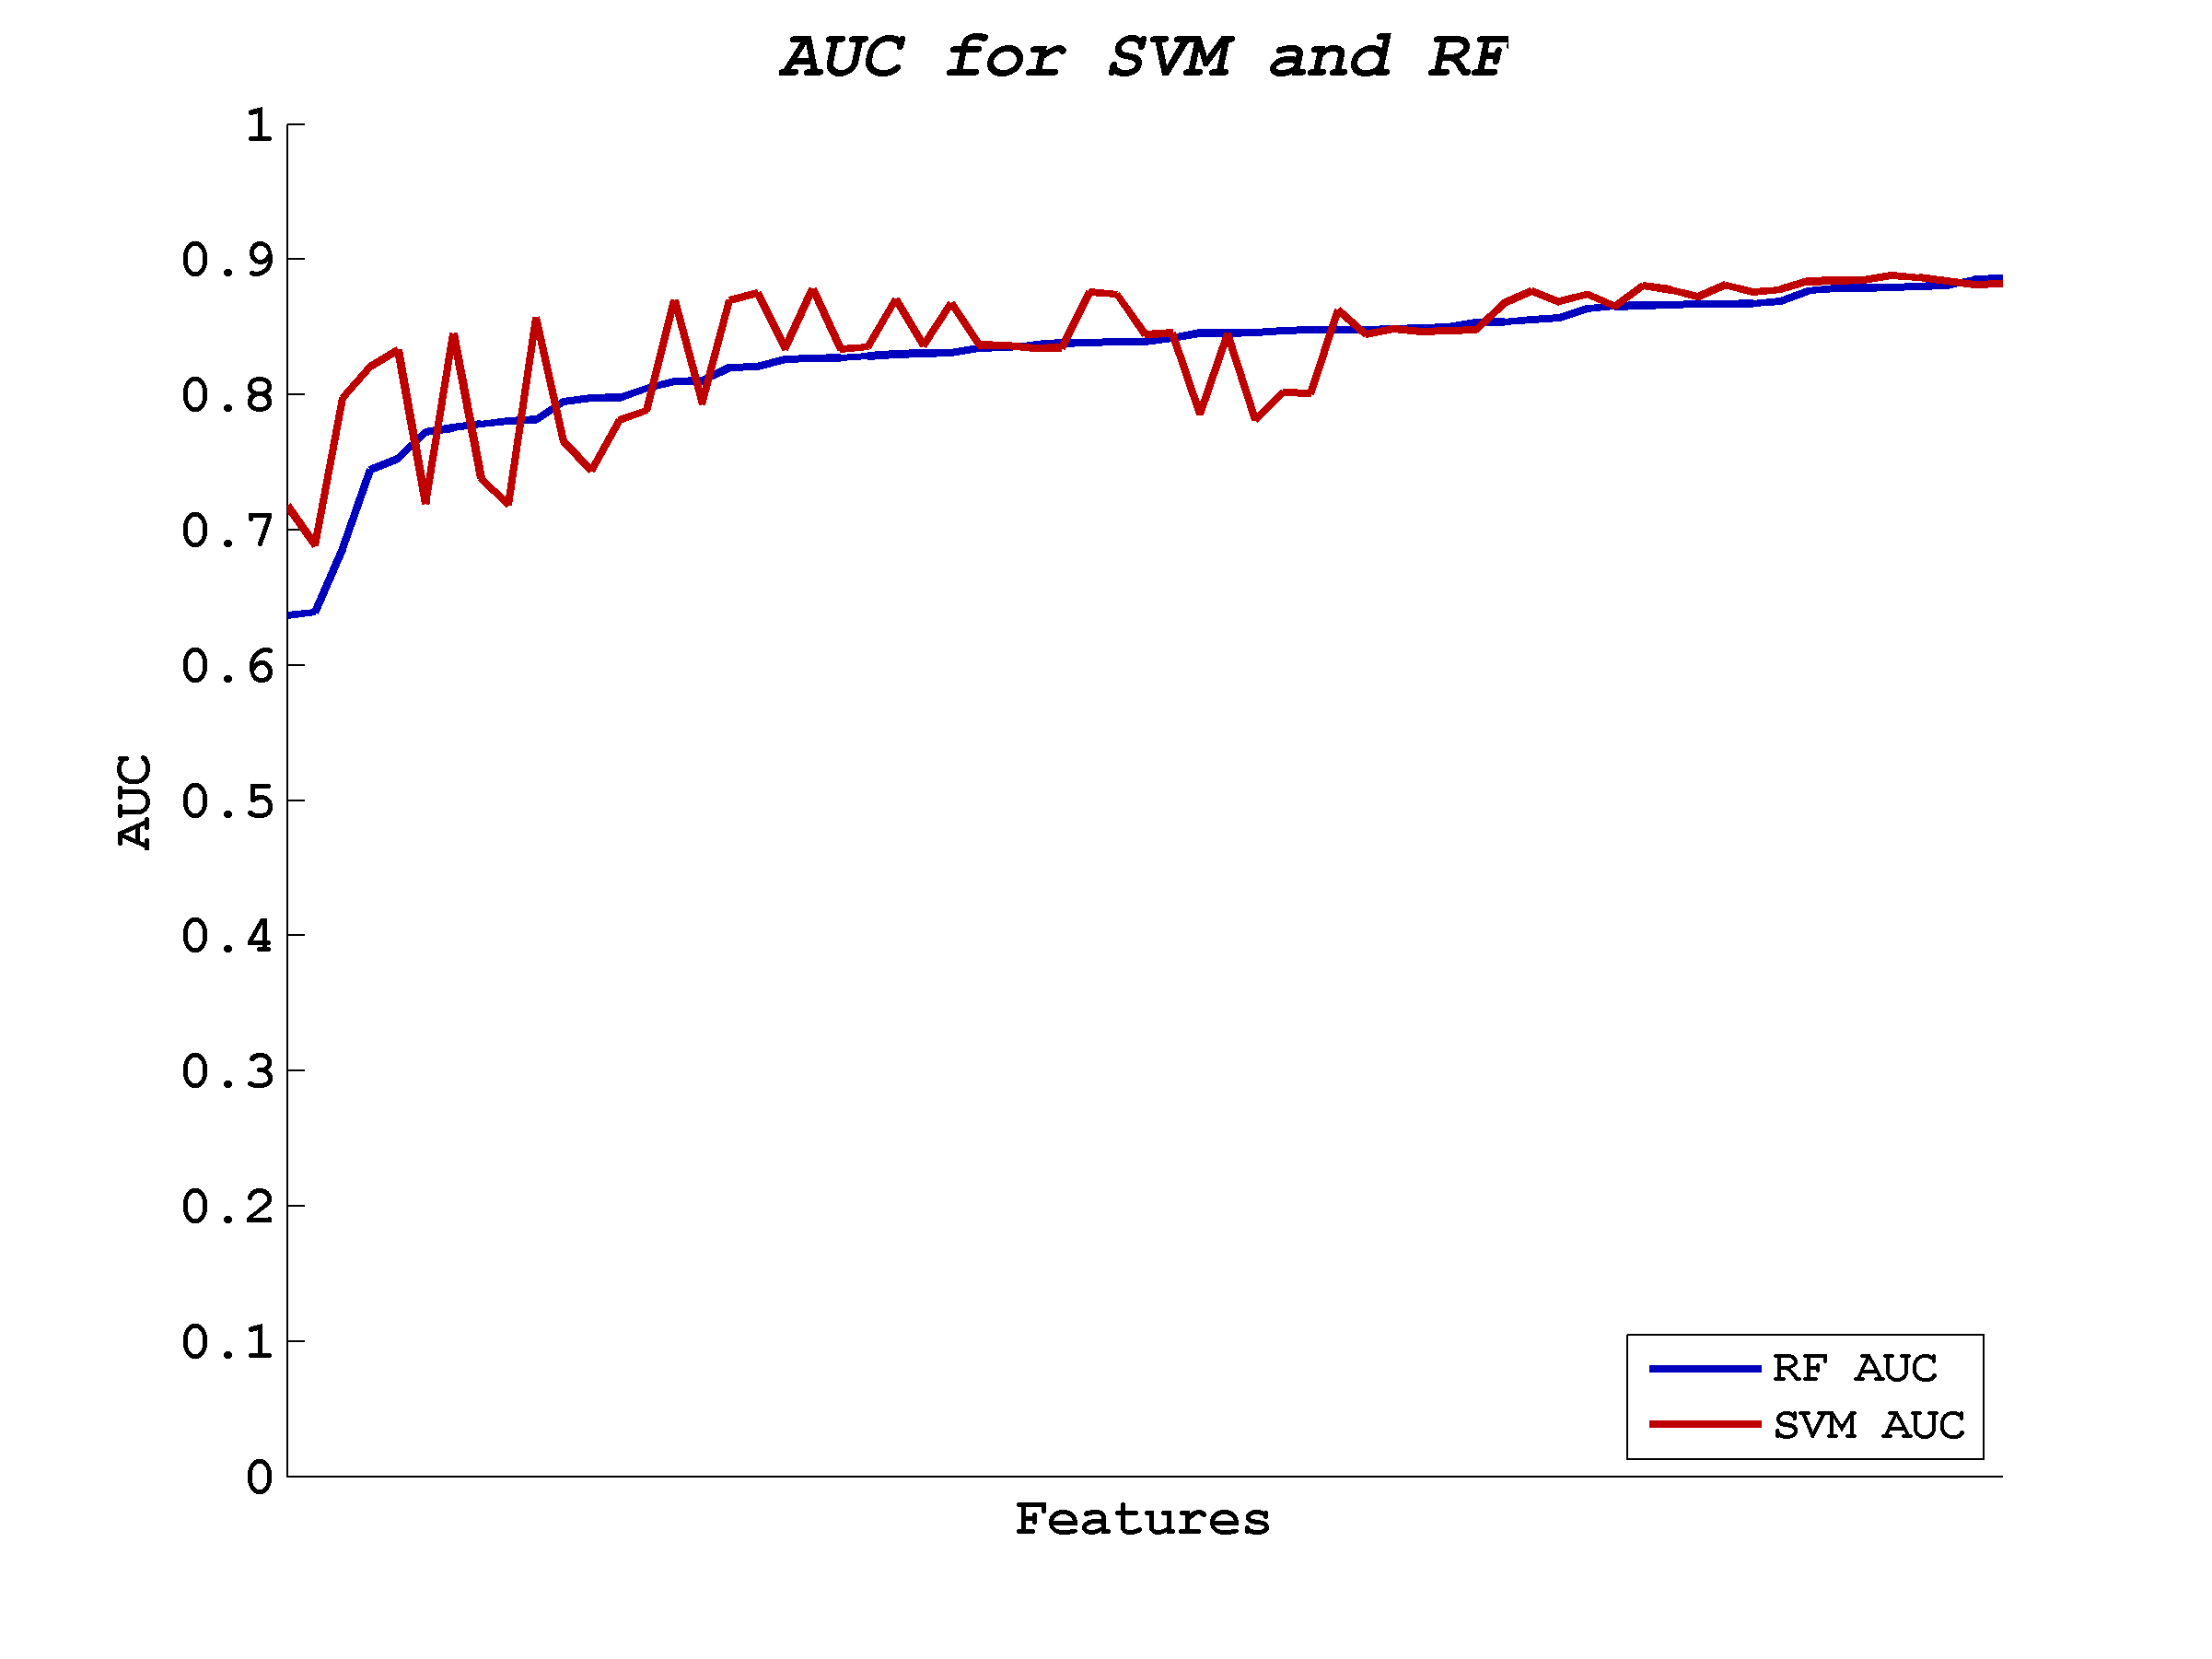
\includegraphics[width=0.46\textwidth]{./images/exp03/MSiVHU_sortAUC.png}
      \label{ch6:fig10:a}
    }
    \hspace{1mm}
    \subfigure[MSiVHU - accuracy]{
      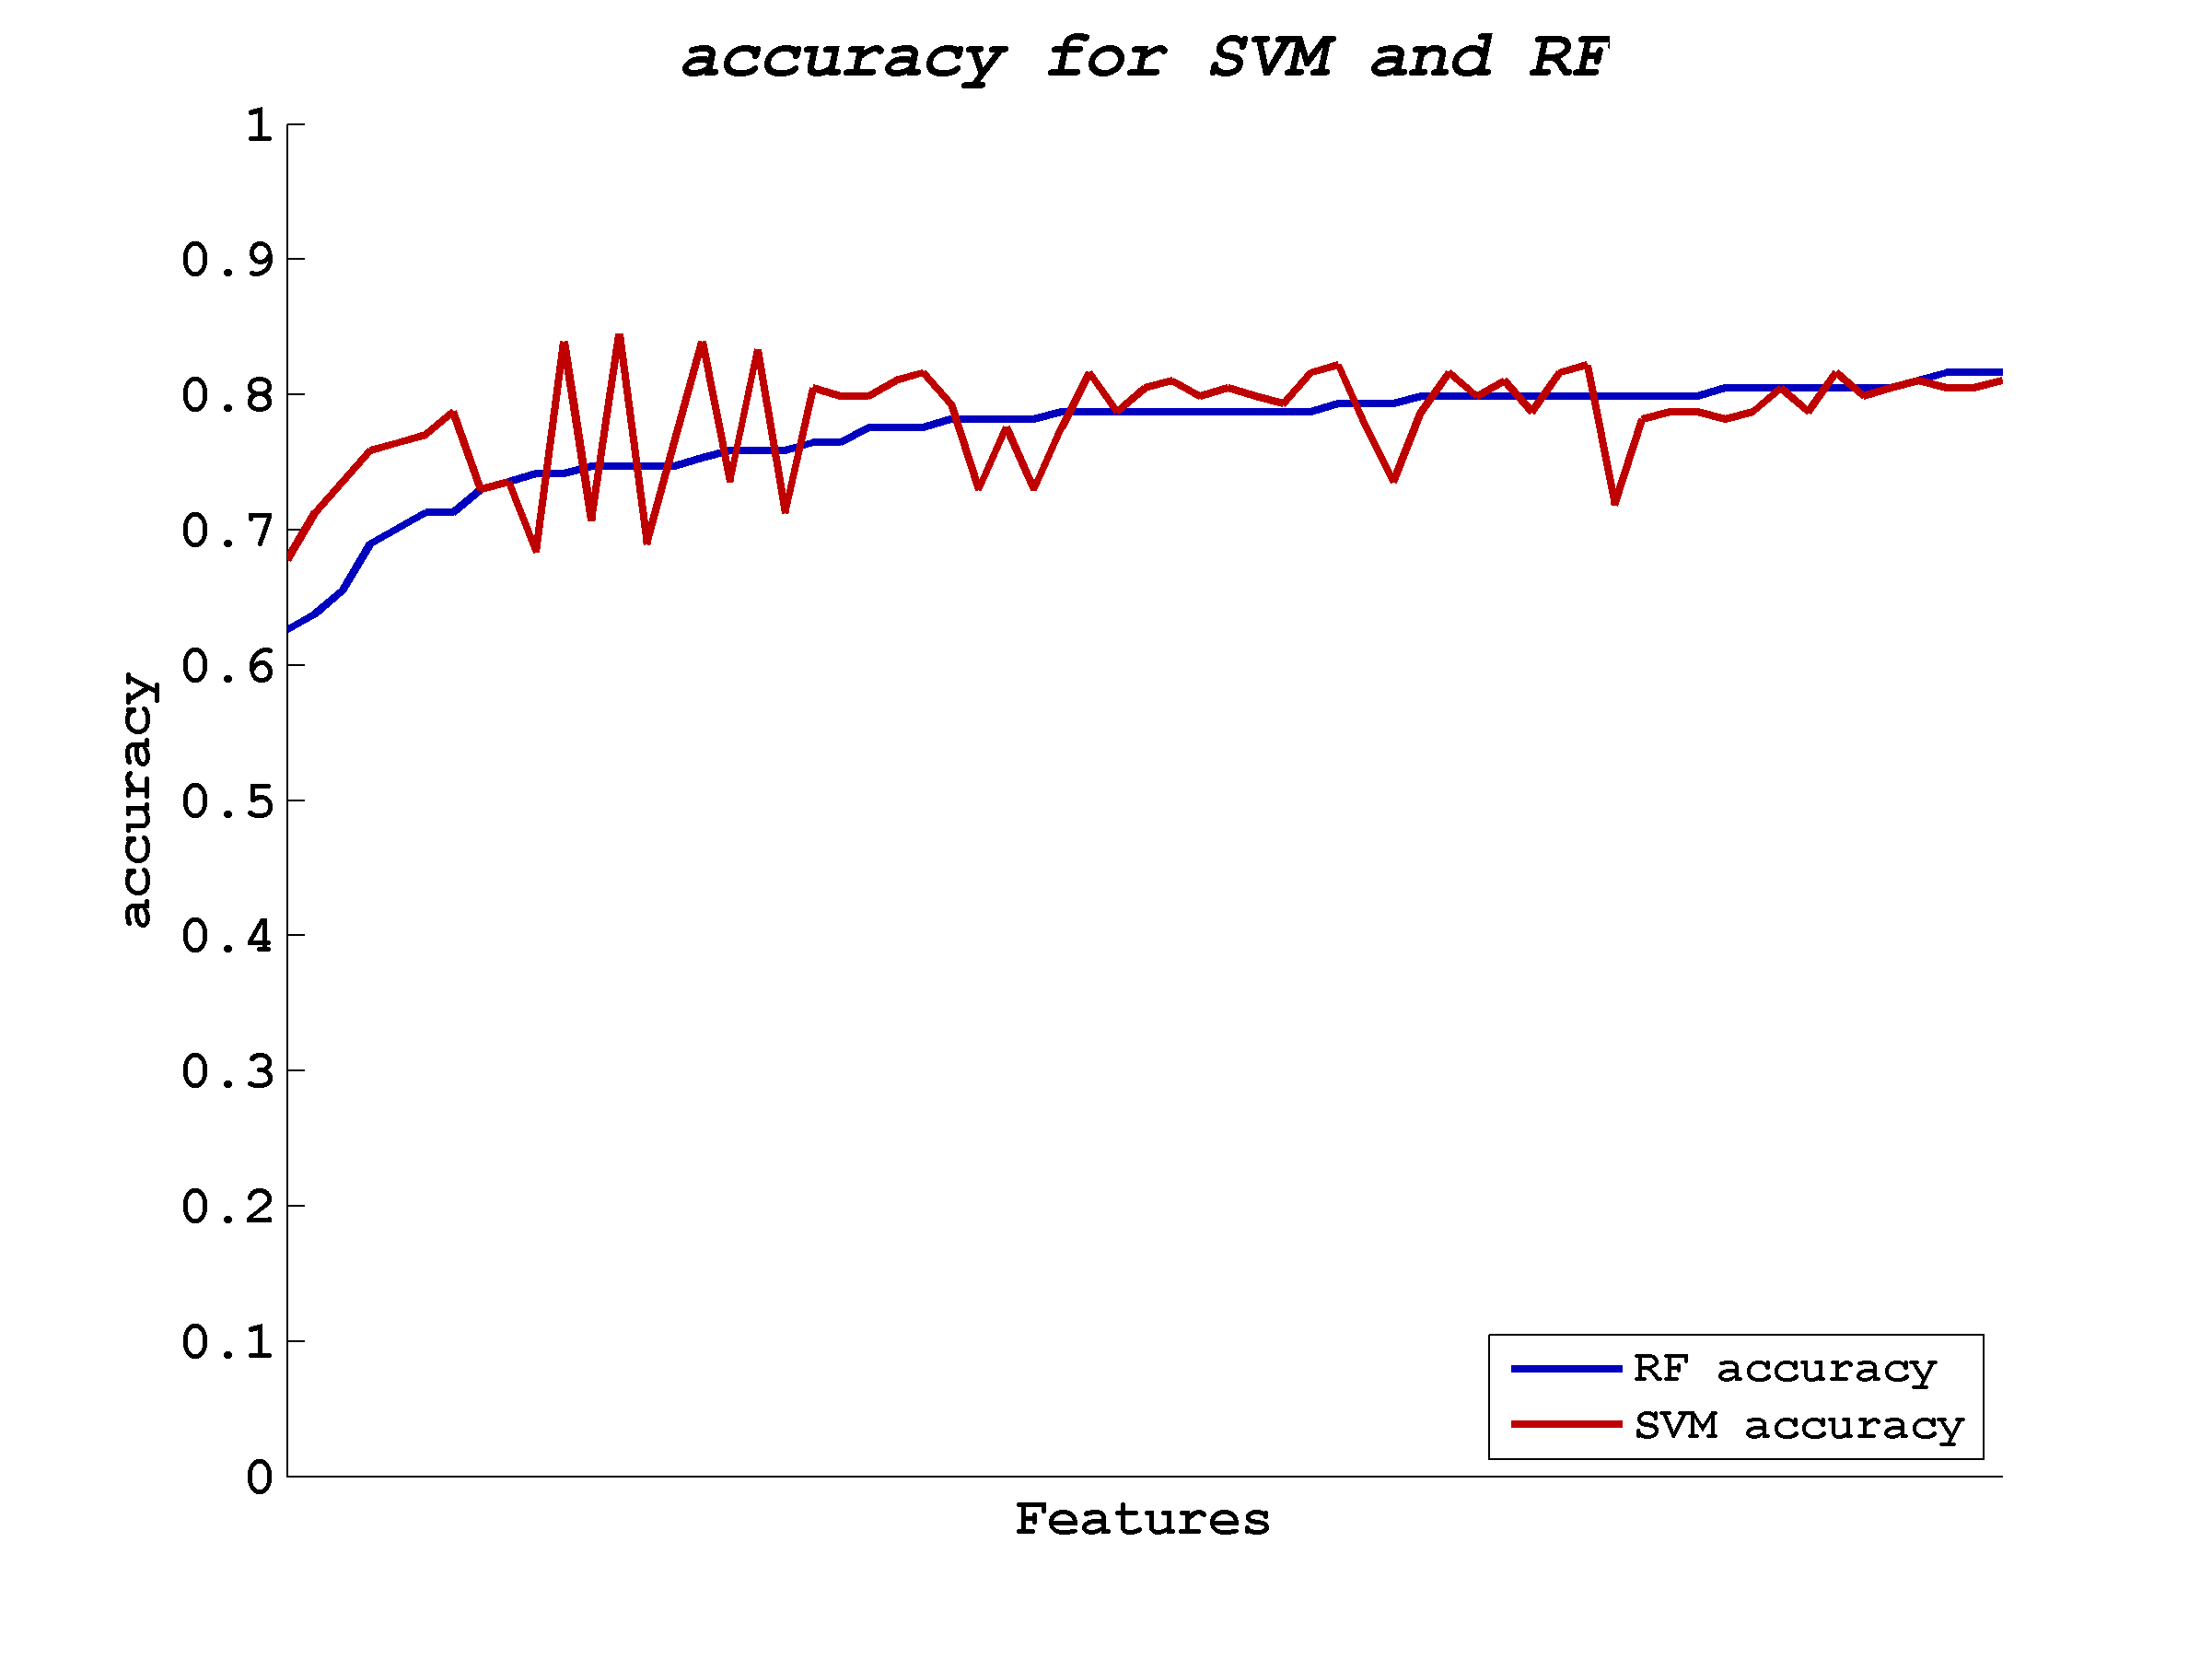
\includegraphics[width=0.46\textwidth]{./images/exp03/MSiVHU_sortAccuracy.png}
      \label{ch6:fig10:b}
    }    
    \caption{Features MSiVHU - overall performances}
    \label{ch6:fig10}
\end{figure}


While it is generally true that the mean performance of the \Gls{RF} classifier is better (in terms of \textit{AUC} and \textit{accuracy}) than the one given by the
\Gls{SVM} classifier, it is not possible to say that \Gls{RF} outperforms \Gls{SVM}. There are many cases in which the \Gls{SVM} performance turns out to be
better, in particular when the LBP$^u2$ feature is involved (see Figure \ref{ch6:fig10}). Nevertheless, the best \Gls{RF} performance is better than \Gls{SVM}'s.


\vspace{0.5cm}

\subsection{Dataset Dimension}

In this experiment we analyzed the effect of the size of the training dataset on the classification performance, in term of selected instances.
To achieve this goal, we repeatedly selected random subsets of the
extended dataset and applied our classifier. To avoid the dependence on the specific selected subset, we run many different experiments with randomly chosen subsets with the same 
size and then we averaged the results.
\\
The Matlab code implemented to run \textit{experiment 4} is listed in \ref{appendixB:exp4}

\vspace{0.5cm}



\subsection{Dataset Dimension: Experimental Results}

Considering fractions of the \textit{training} dataset ranging $1\%$ \textrightarrow $100\%$, we performed the classification on the
whole \textit{evaluation} set having trained the classifier o a randomly selected subset. In order to reduce the risk of biases due to
a specific subset, we made different trials, selecting at each time the training dataset. We used the following empirical rule to decide 
the number of trials in function of the subset size:

\begin{equation}
\label{ch6:eq1}
 \frac{\textrm{subset-size}}{\textrm{trial}} \cdot \left( \sharp \ \textrm{of trials} \right) \approx 3
\end{equation}

Equation \ref{ch6:eq1} brings to the number of trials illustrated in Figure \ref{ch6:fig11}.

\begin{figure}[!hbf]
 \begin{center}
  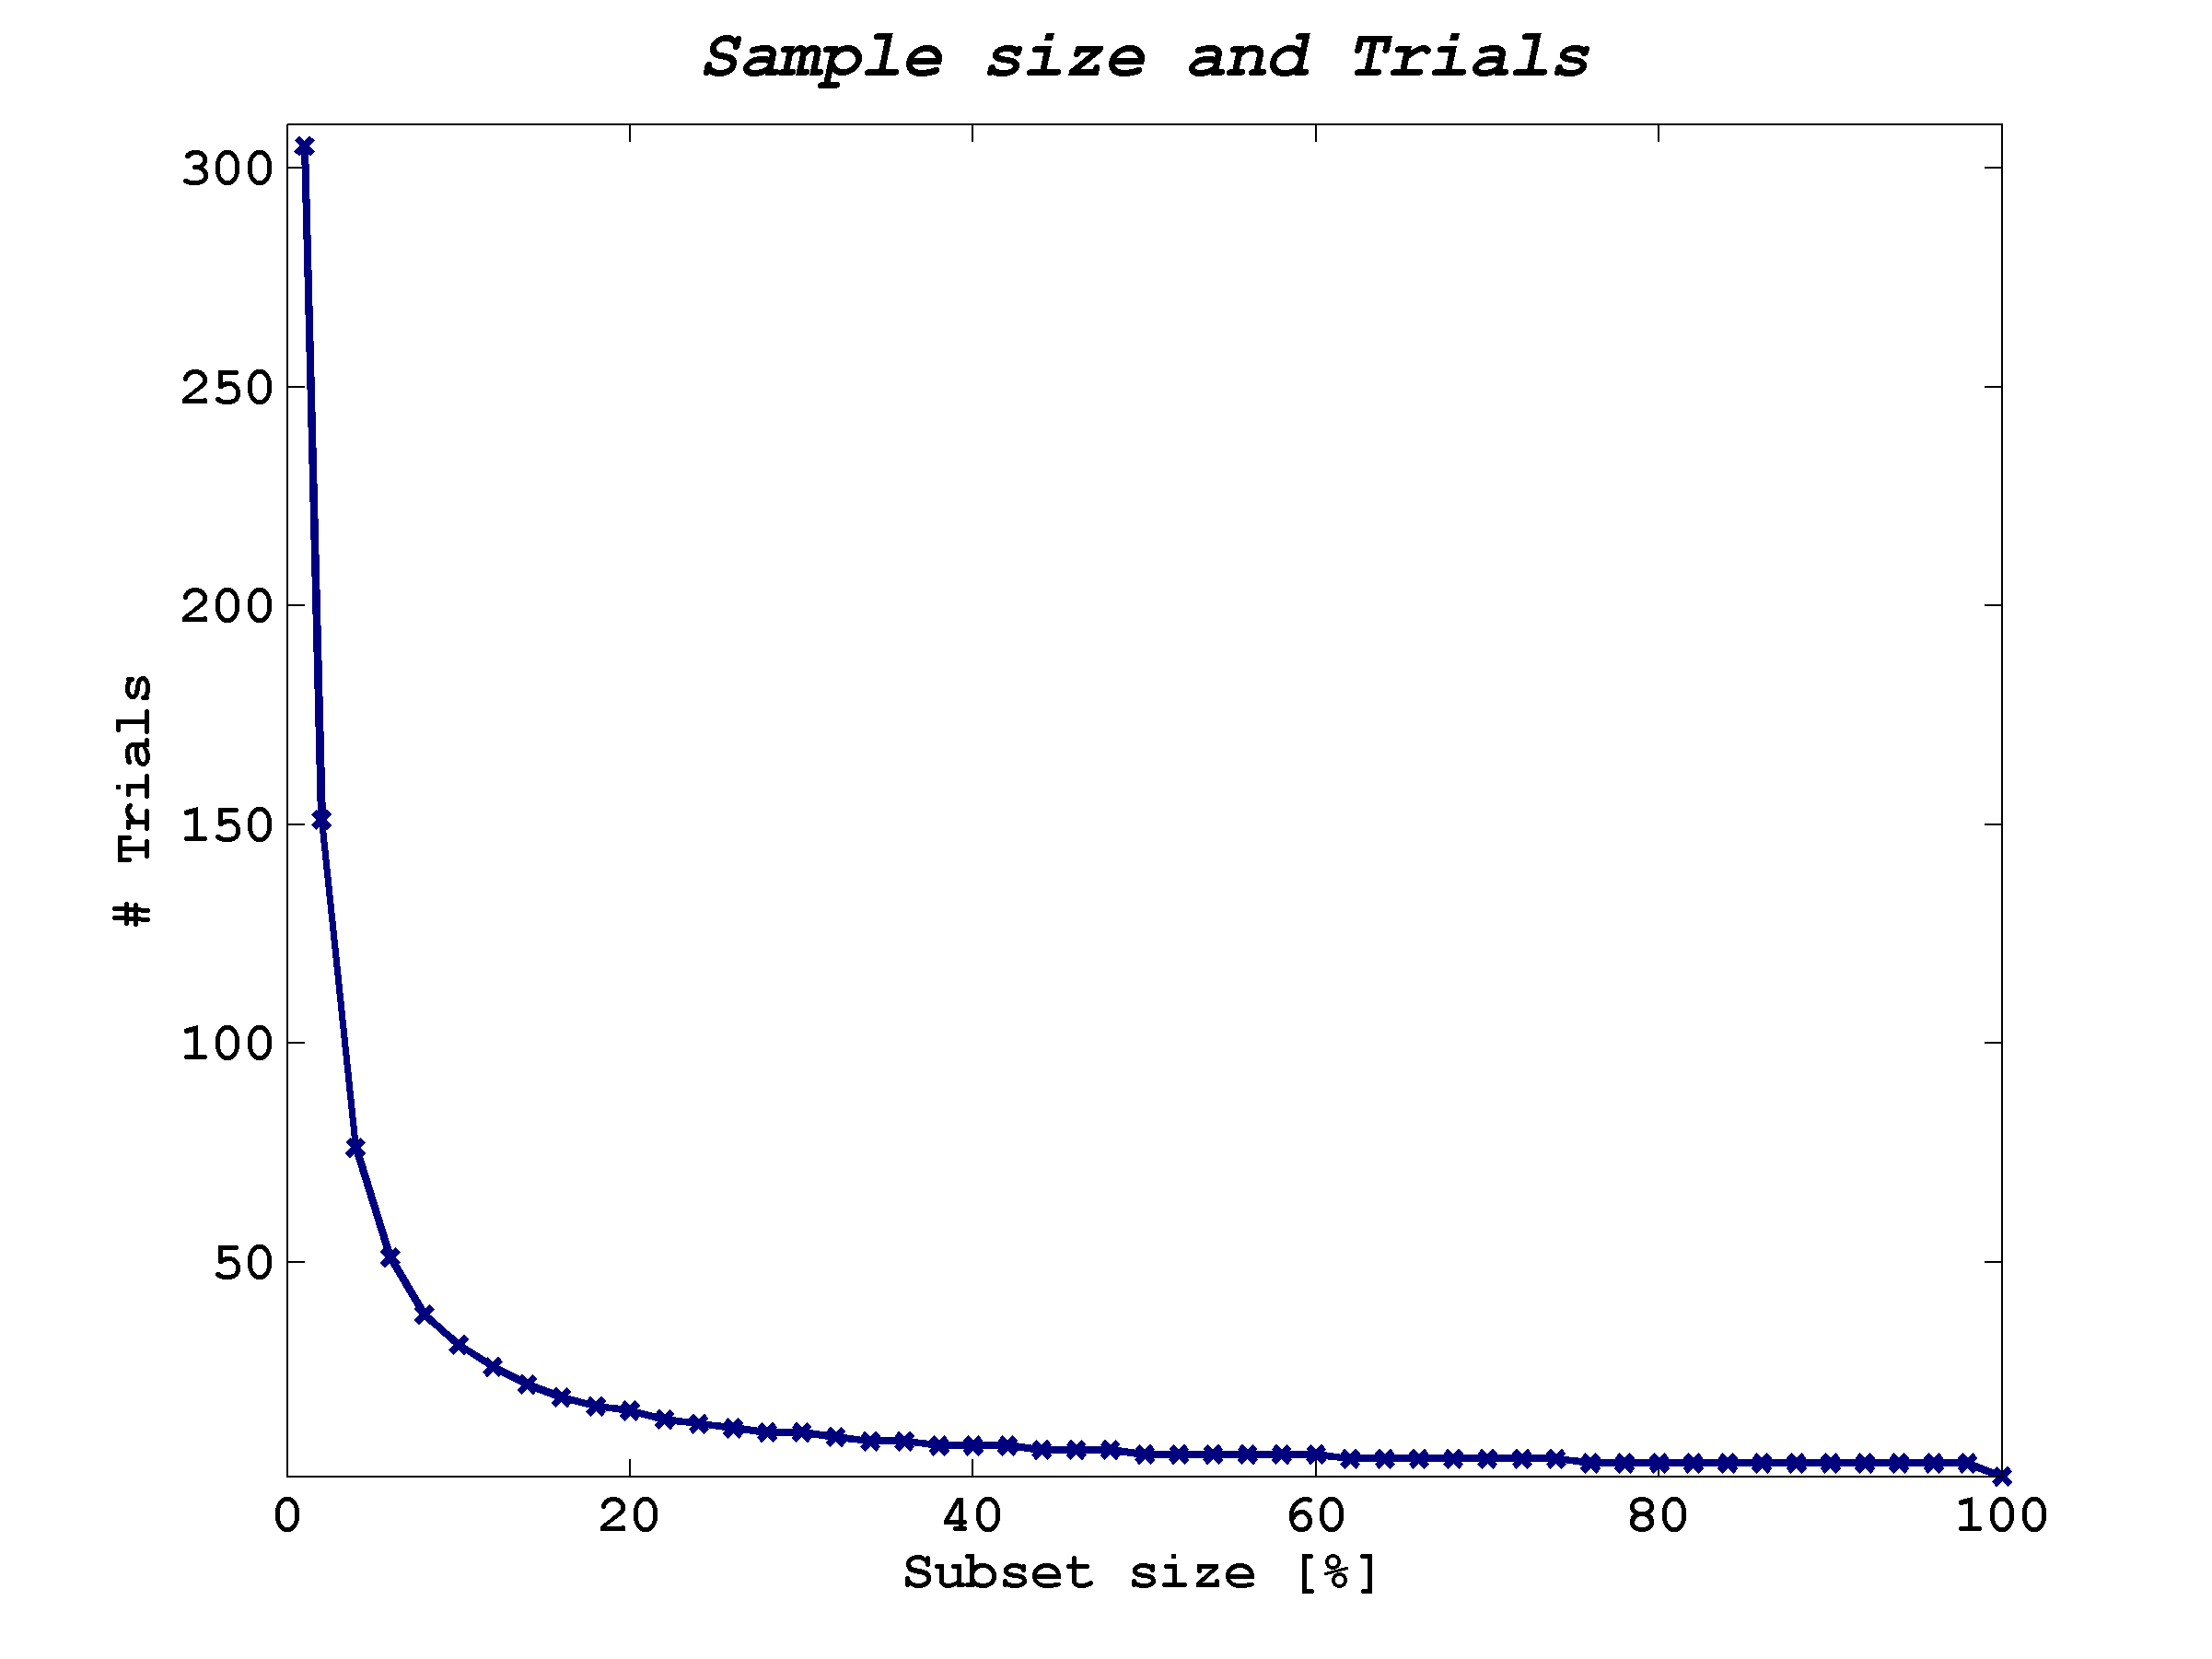
\includegraphics[width=0.75\textwidth]{./images/exp04/iVHL_trials.png}
  \caption[subset size and trials]{Subset size and number of trials}
  \label{ch6:fig11}
 \end{center}
\end{figure}

We run experiments on different sets of features that performed well in previous tests (not necessarily the best ones): \texttt{iVHL}, \texttt{MiVHU} and \texttt{MSVHR}.
We initially used used both of our classifiers. However, it emerged that, with some combination of instances, the \Gls{SVM} was unable to find a proper solution.
For this reason we preferred to focus on the performances of the \Gls{RF} classifier, which contextually turned out to be more robust.\\
As usual we considered, as a metric of performance, \textit{AUC} and \textit{accuracy}.

\vspace{0.5cm}

\subsubsection{Classifier: RF - Features \texttt{iVHL}}

The results are shown in Figure \ref{ch6:fig12}, where the continuous line represents the average of the performance, and the \textasteriskcentered represent the
single classification result.

\begin{figure}[!htb]
  \centering
    \subfigure[RF iVHL - AUC]{
      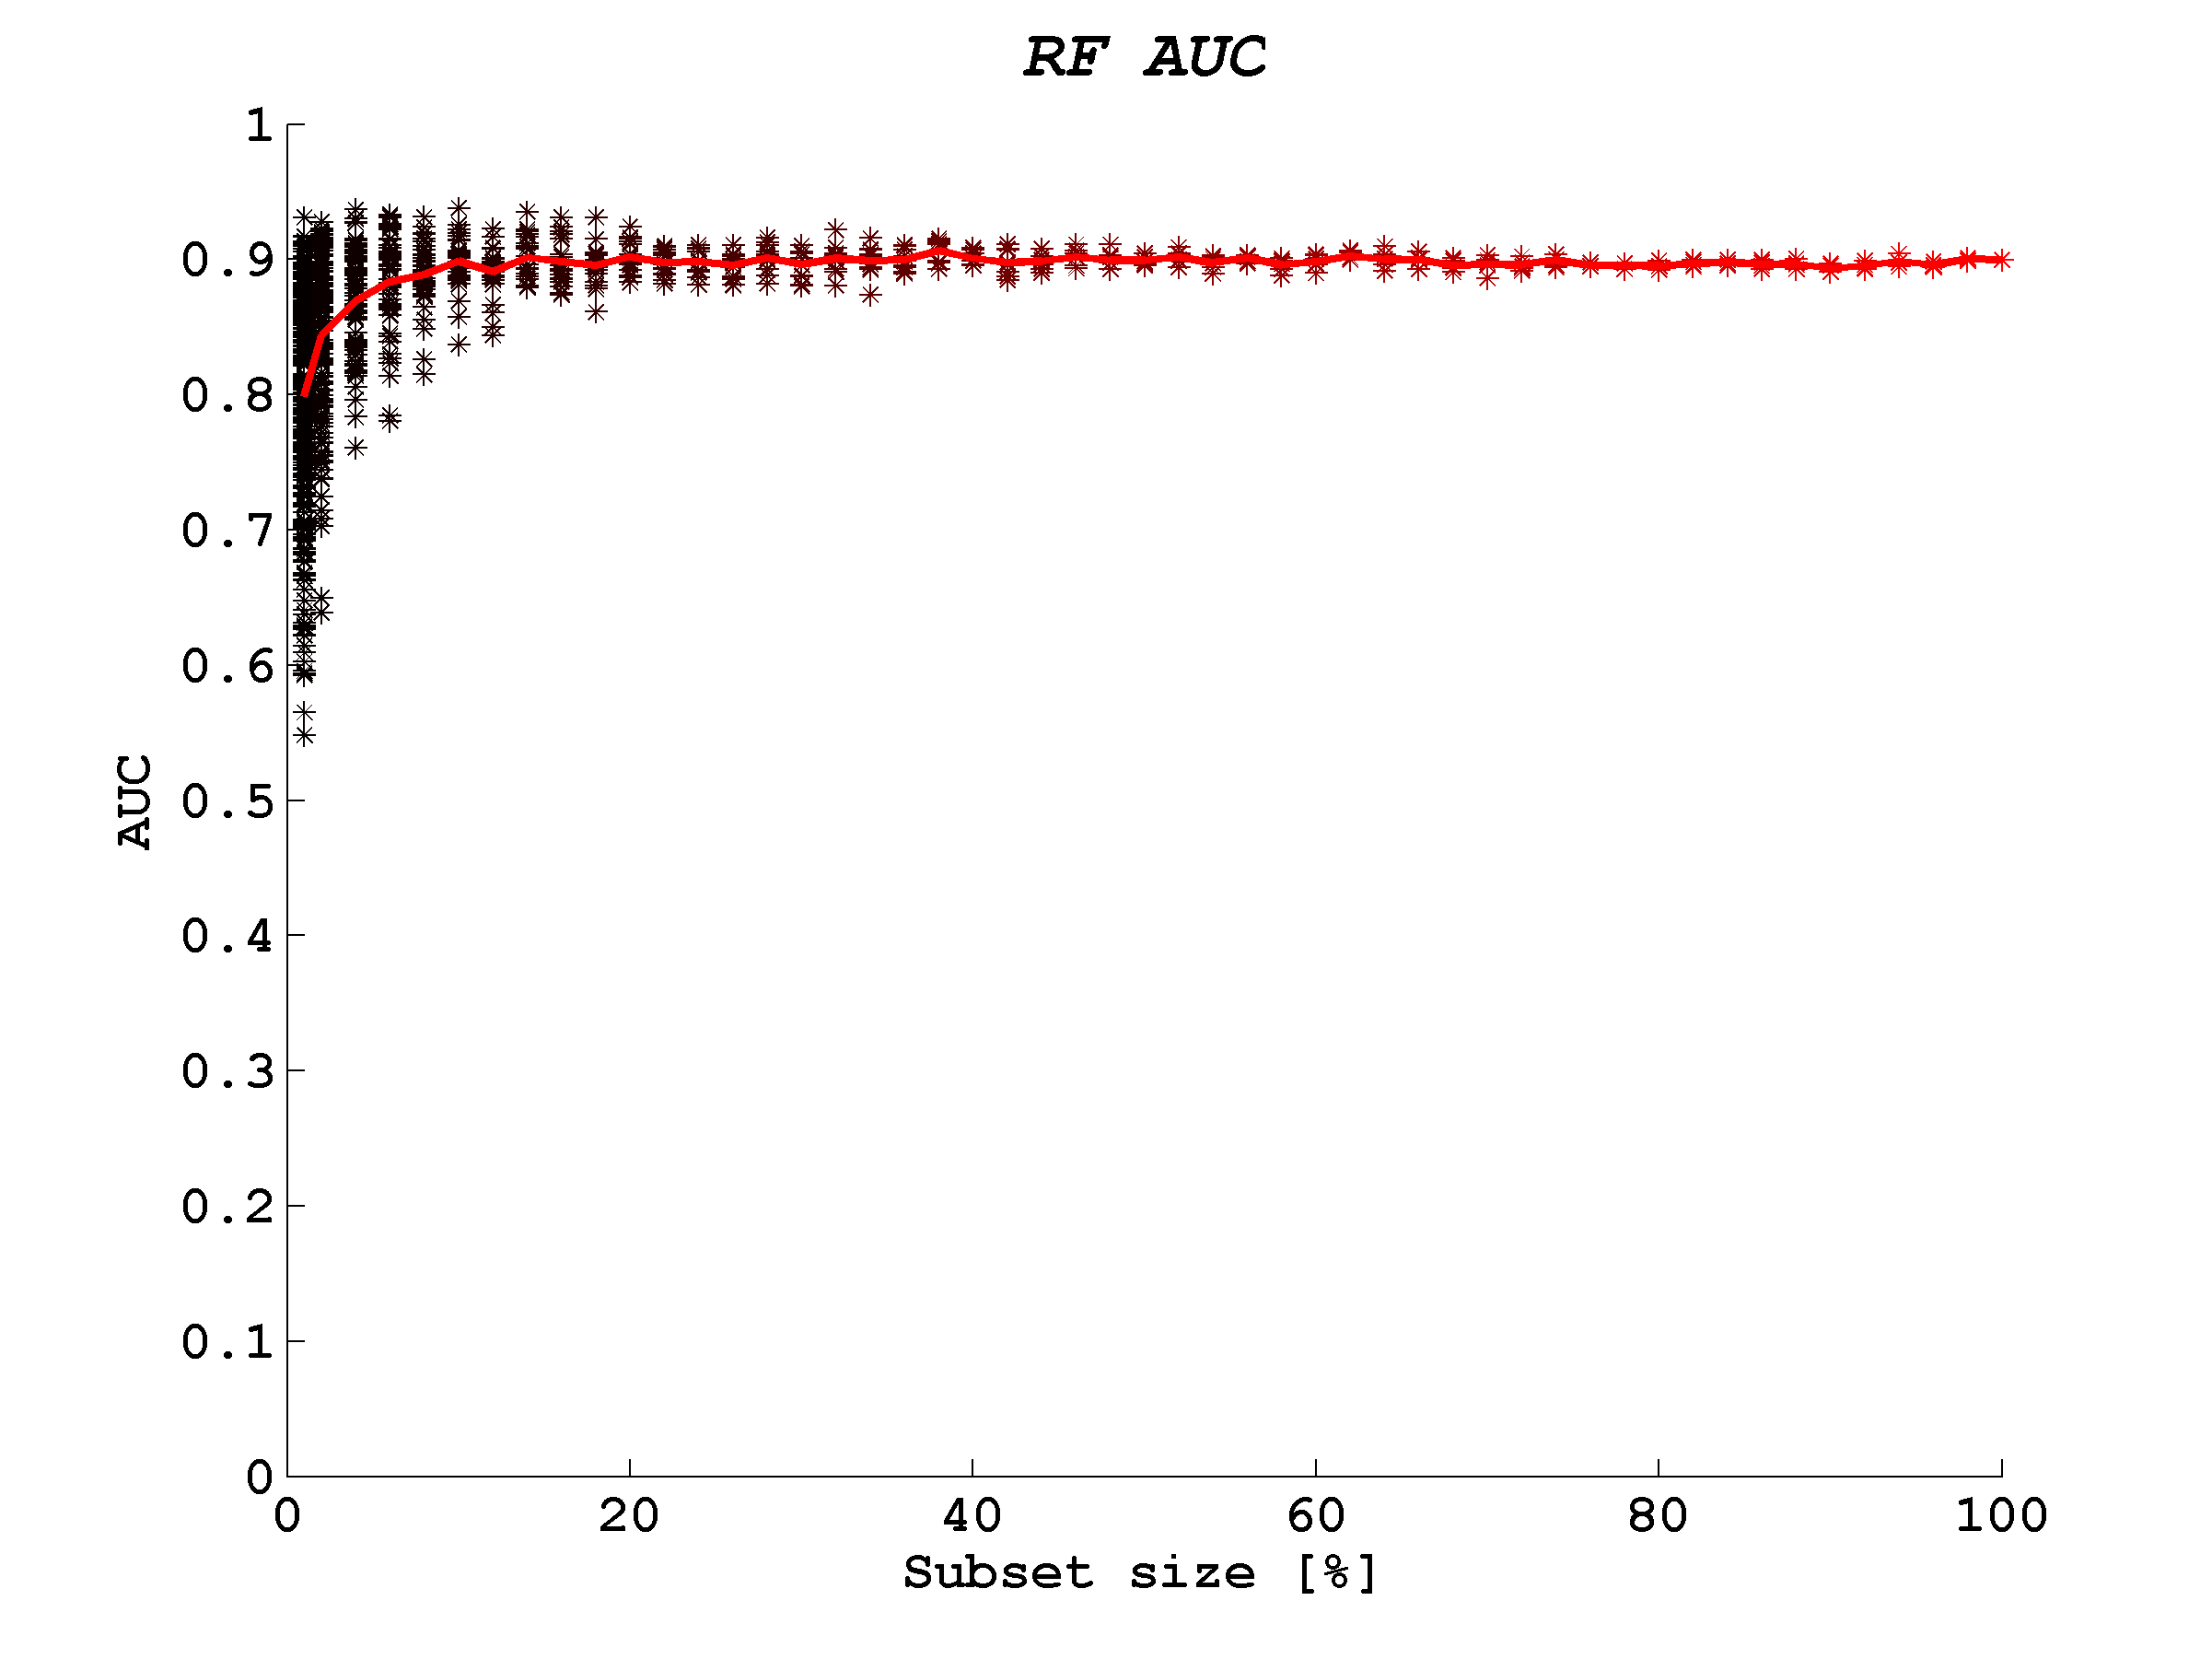
\includegraphics[width=0.75\textwidth]{./images/exp04/iVHL_RF_AUC.png}
      \label{ch6:fig12:a}
    }
    \\
    \subfigure[RF iVHL - accuracy]{
      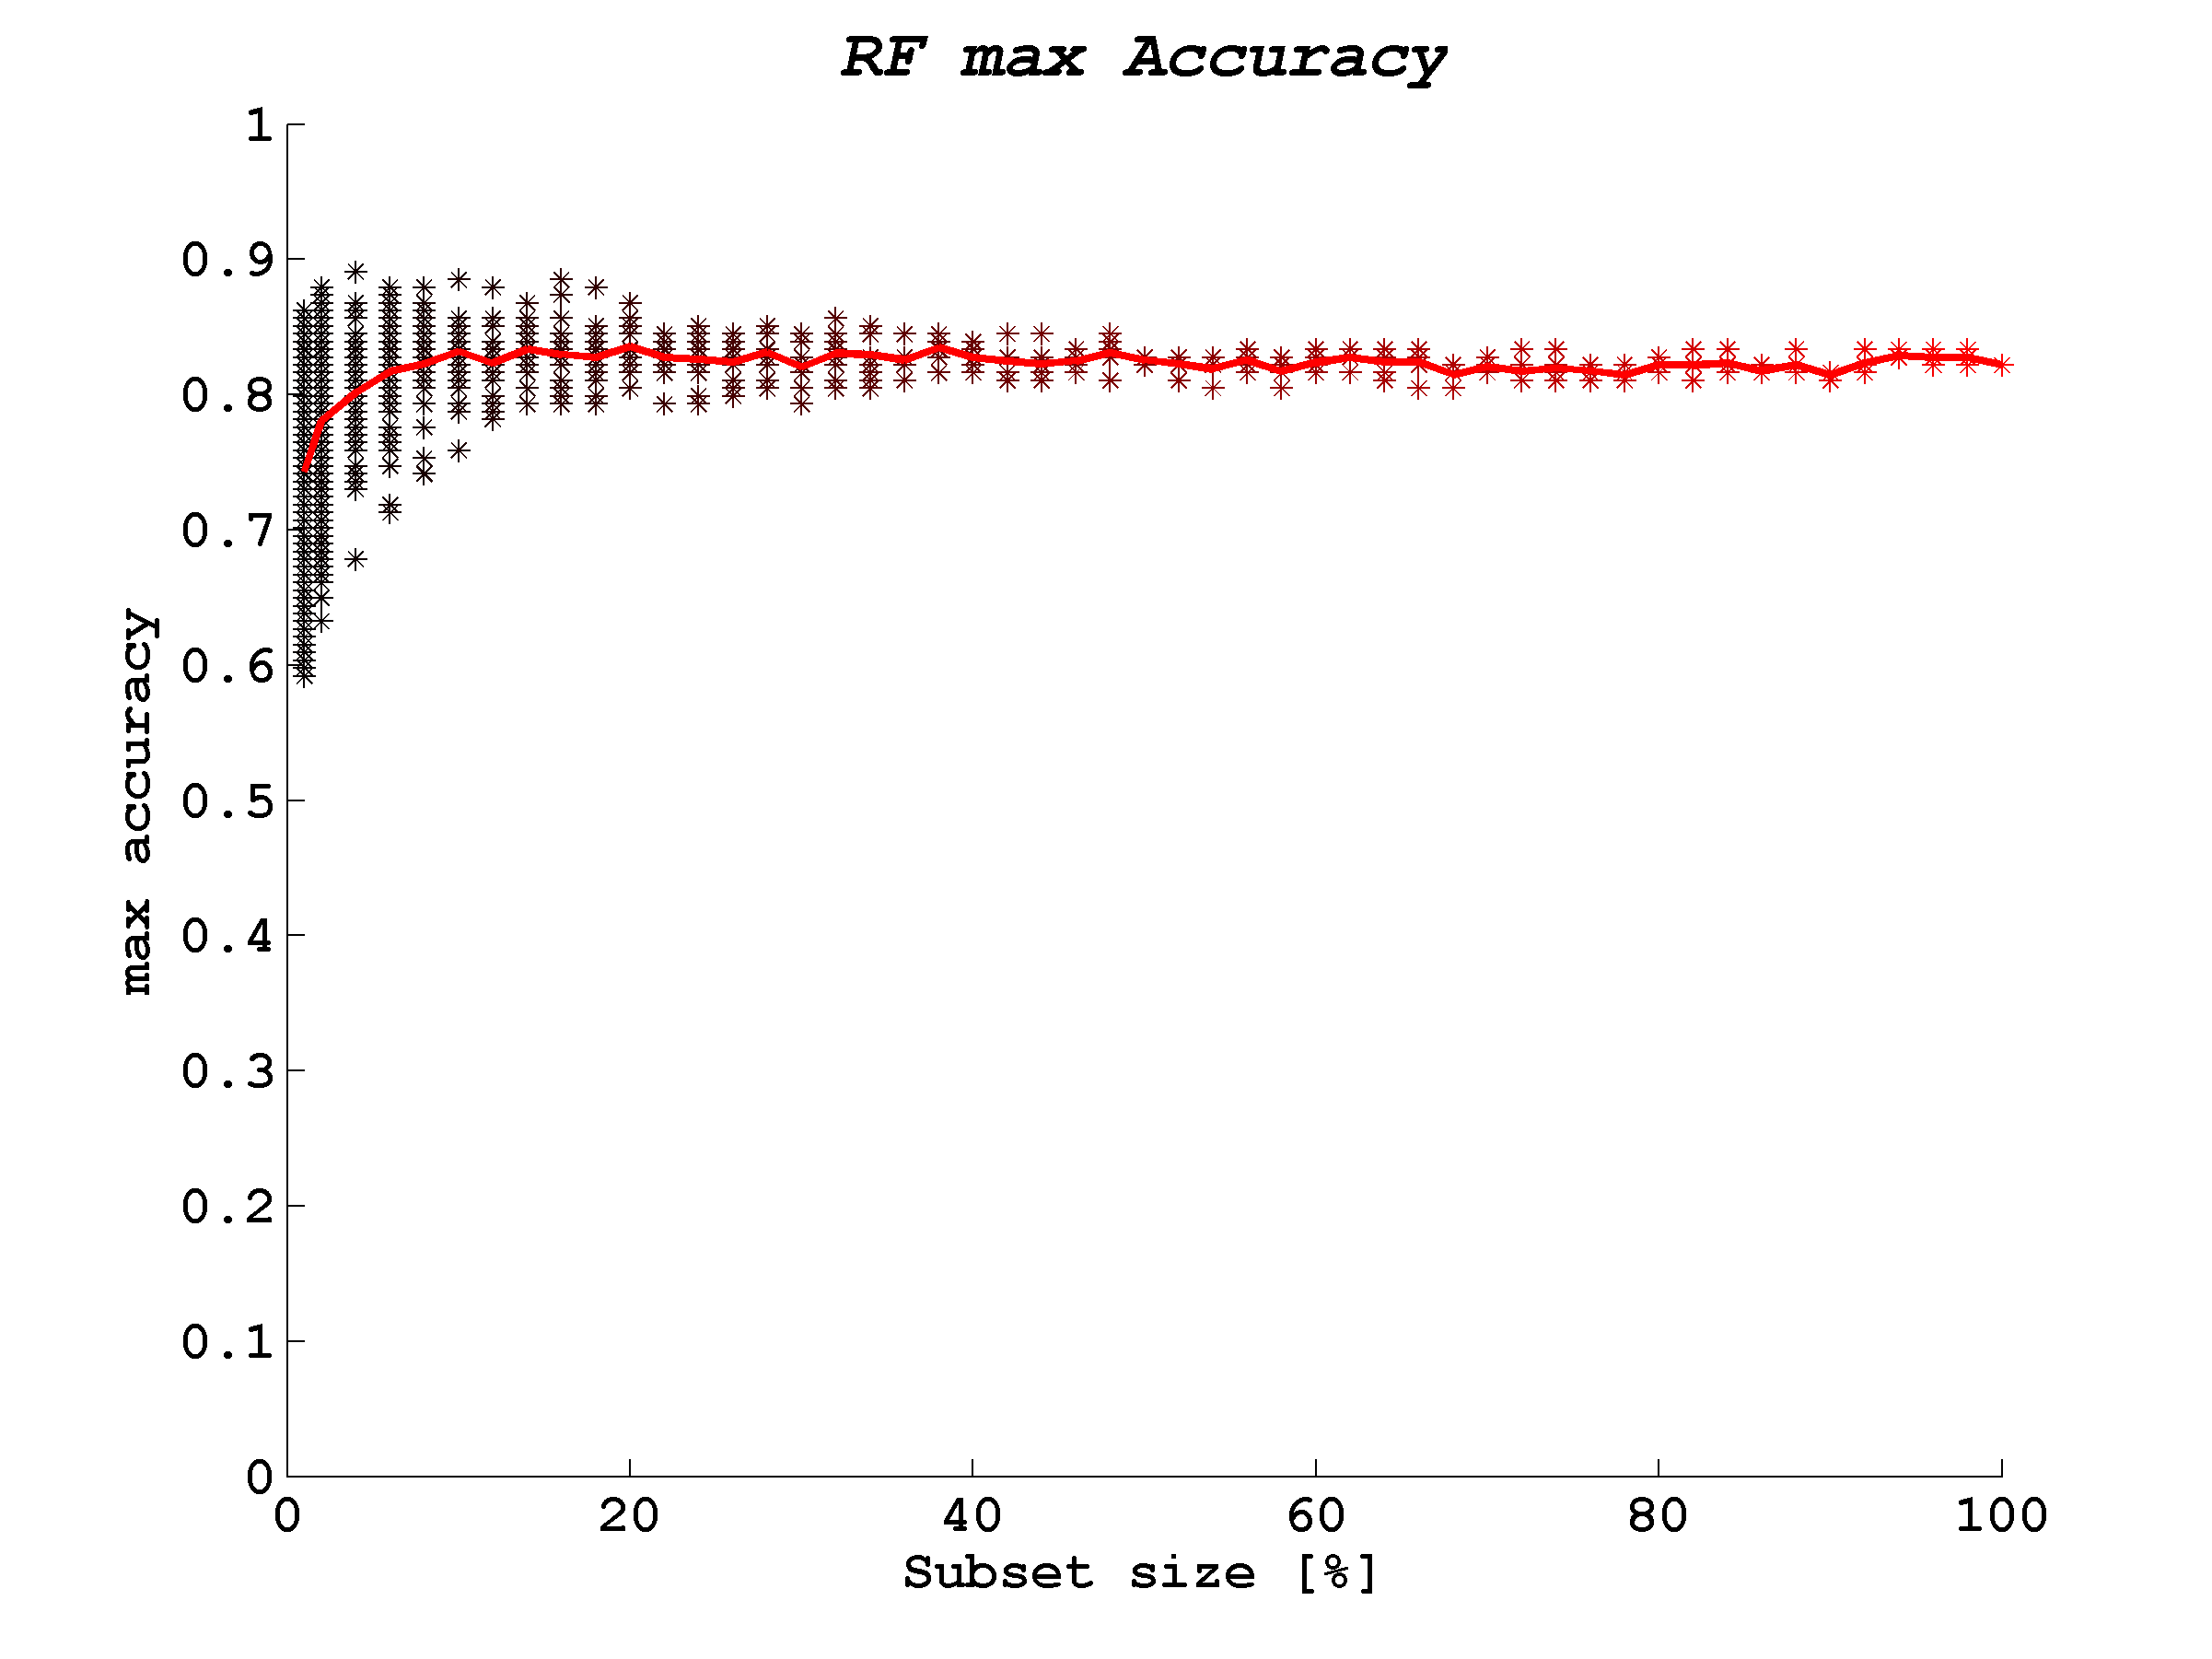
\includegraphics[width=0.75\textwidth]{./images/exp04/iVHL_RF_acc.png}
      \label{ch6:fig12:b}
    }    
    \caption{Features iVHL - sample size}
    \label{ch6:fig12}
\end{figure}

It is apparent that, on one side, the performance grows with the subset size, and on the other side the variance of the performance reduces.
Once the $20\%$ of the dataset size is reached, the average performance remains steady, but it is necessary to reach about the $50\%$ of the dataset to
have small variability of the data.

\vspace{0.5cm}

\subsubsection{Classifier: RF - Features \texttt{MiVHU}}

Figure \ref{ch6:fig13}, shows the results with \texttt{MiVHU} feature set.

\begin{figure}[!htb]
  \centering
    \subfigure[RF MiVHU - AUC]{
      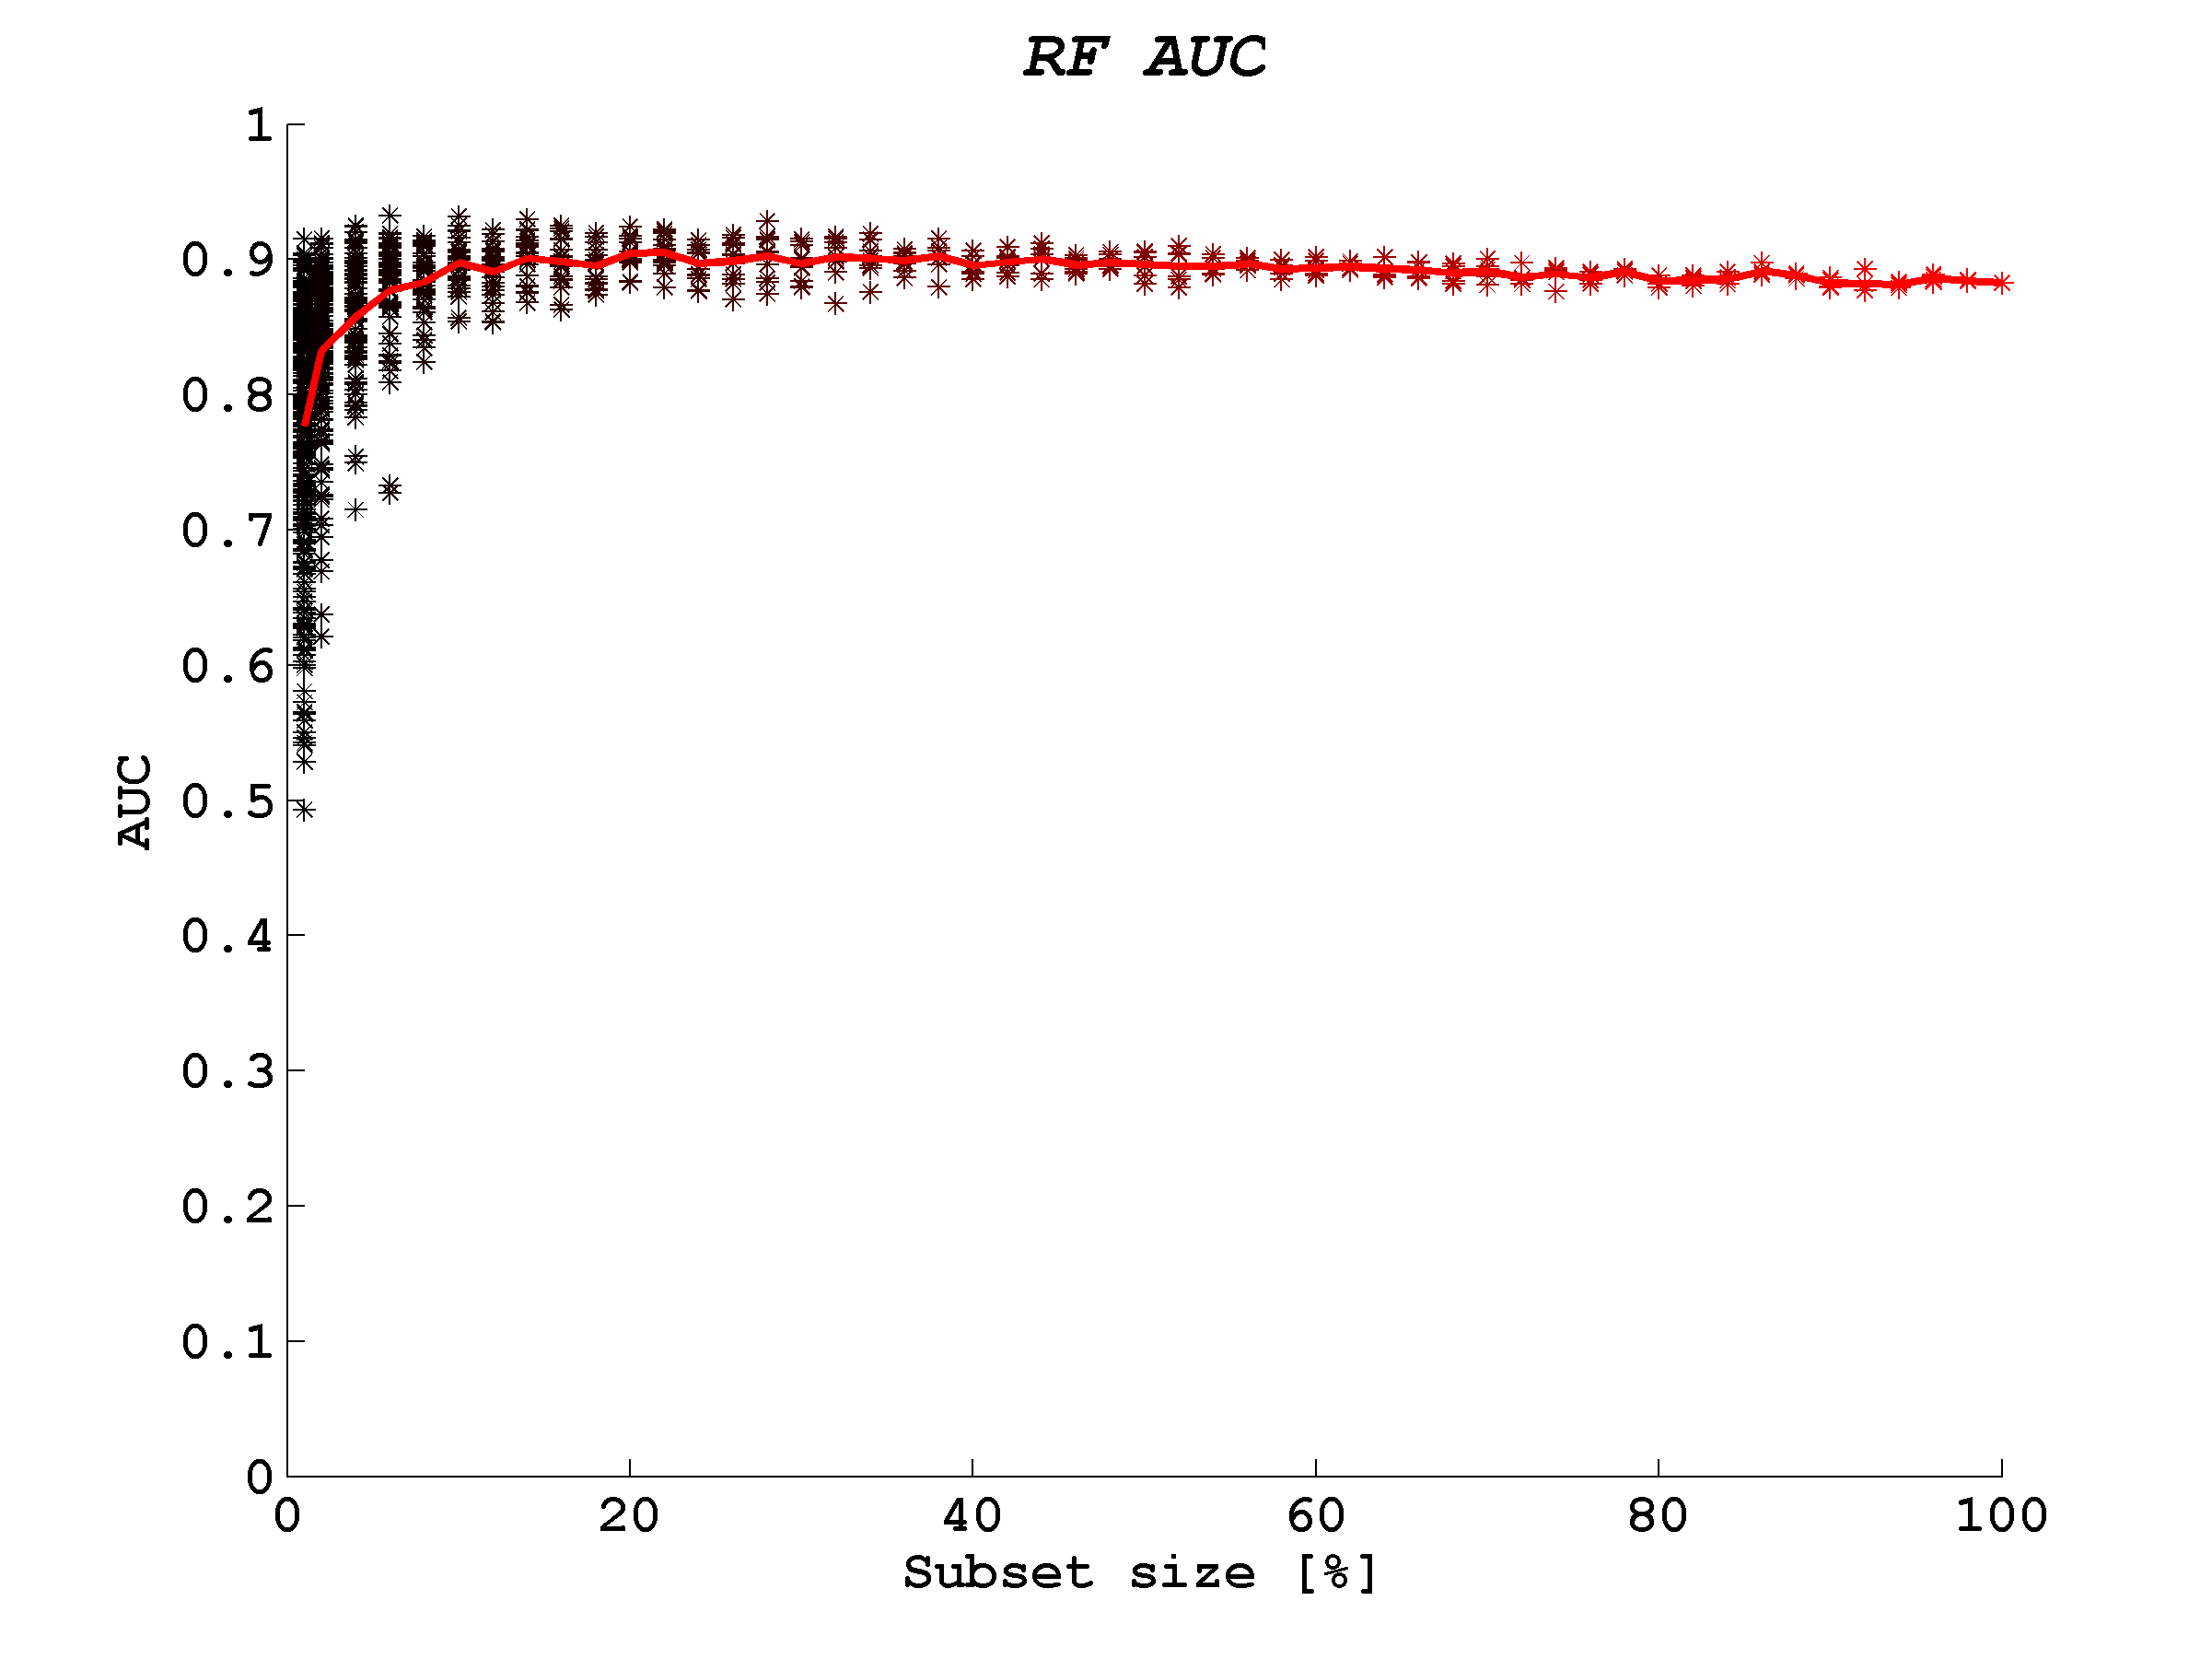
\includegraphics[width=0.75\textwidth]{./images/exp04/MiVHU_RF_AUC.png}
      \label{ch6:fig13:a}
    }
    \\
    \subfigure[RF MiVHU - accuracy]{
      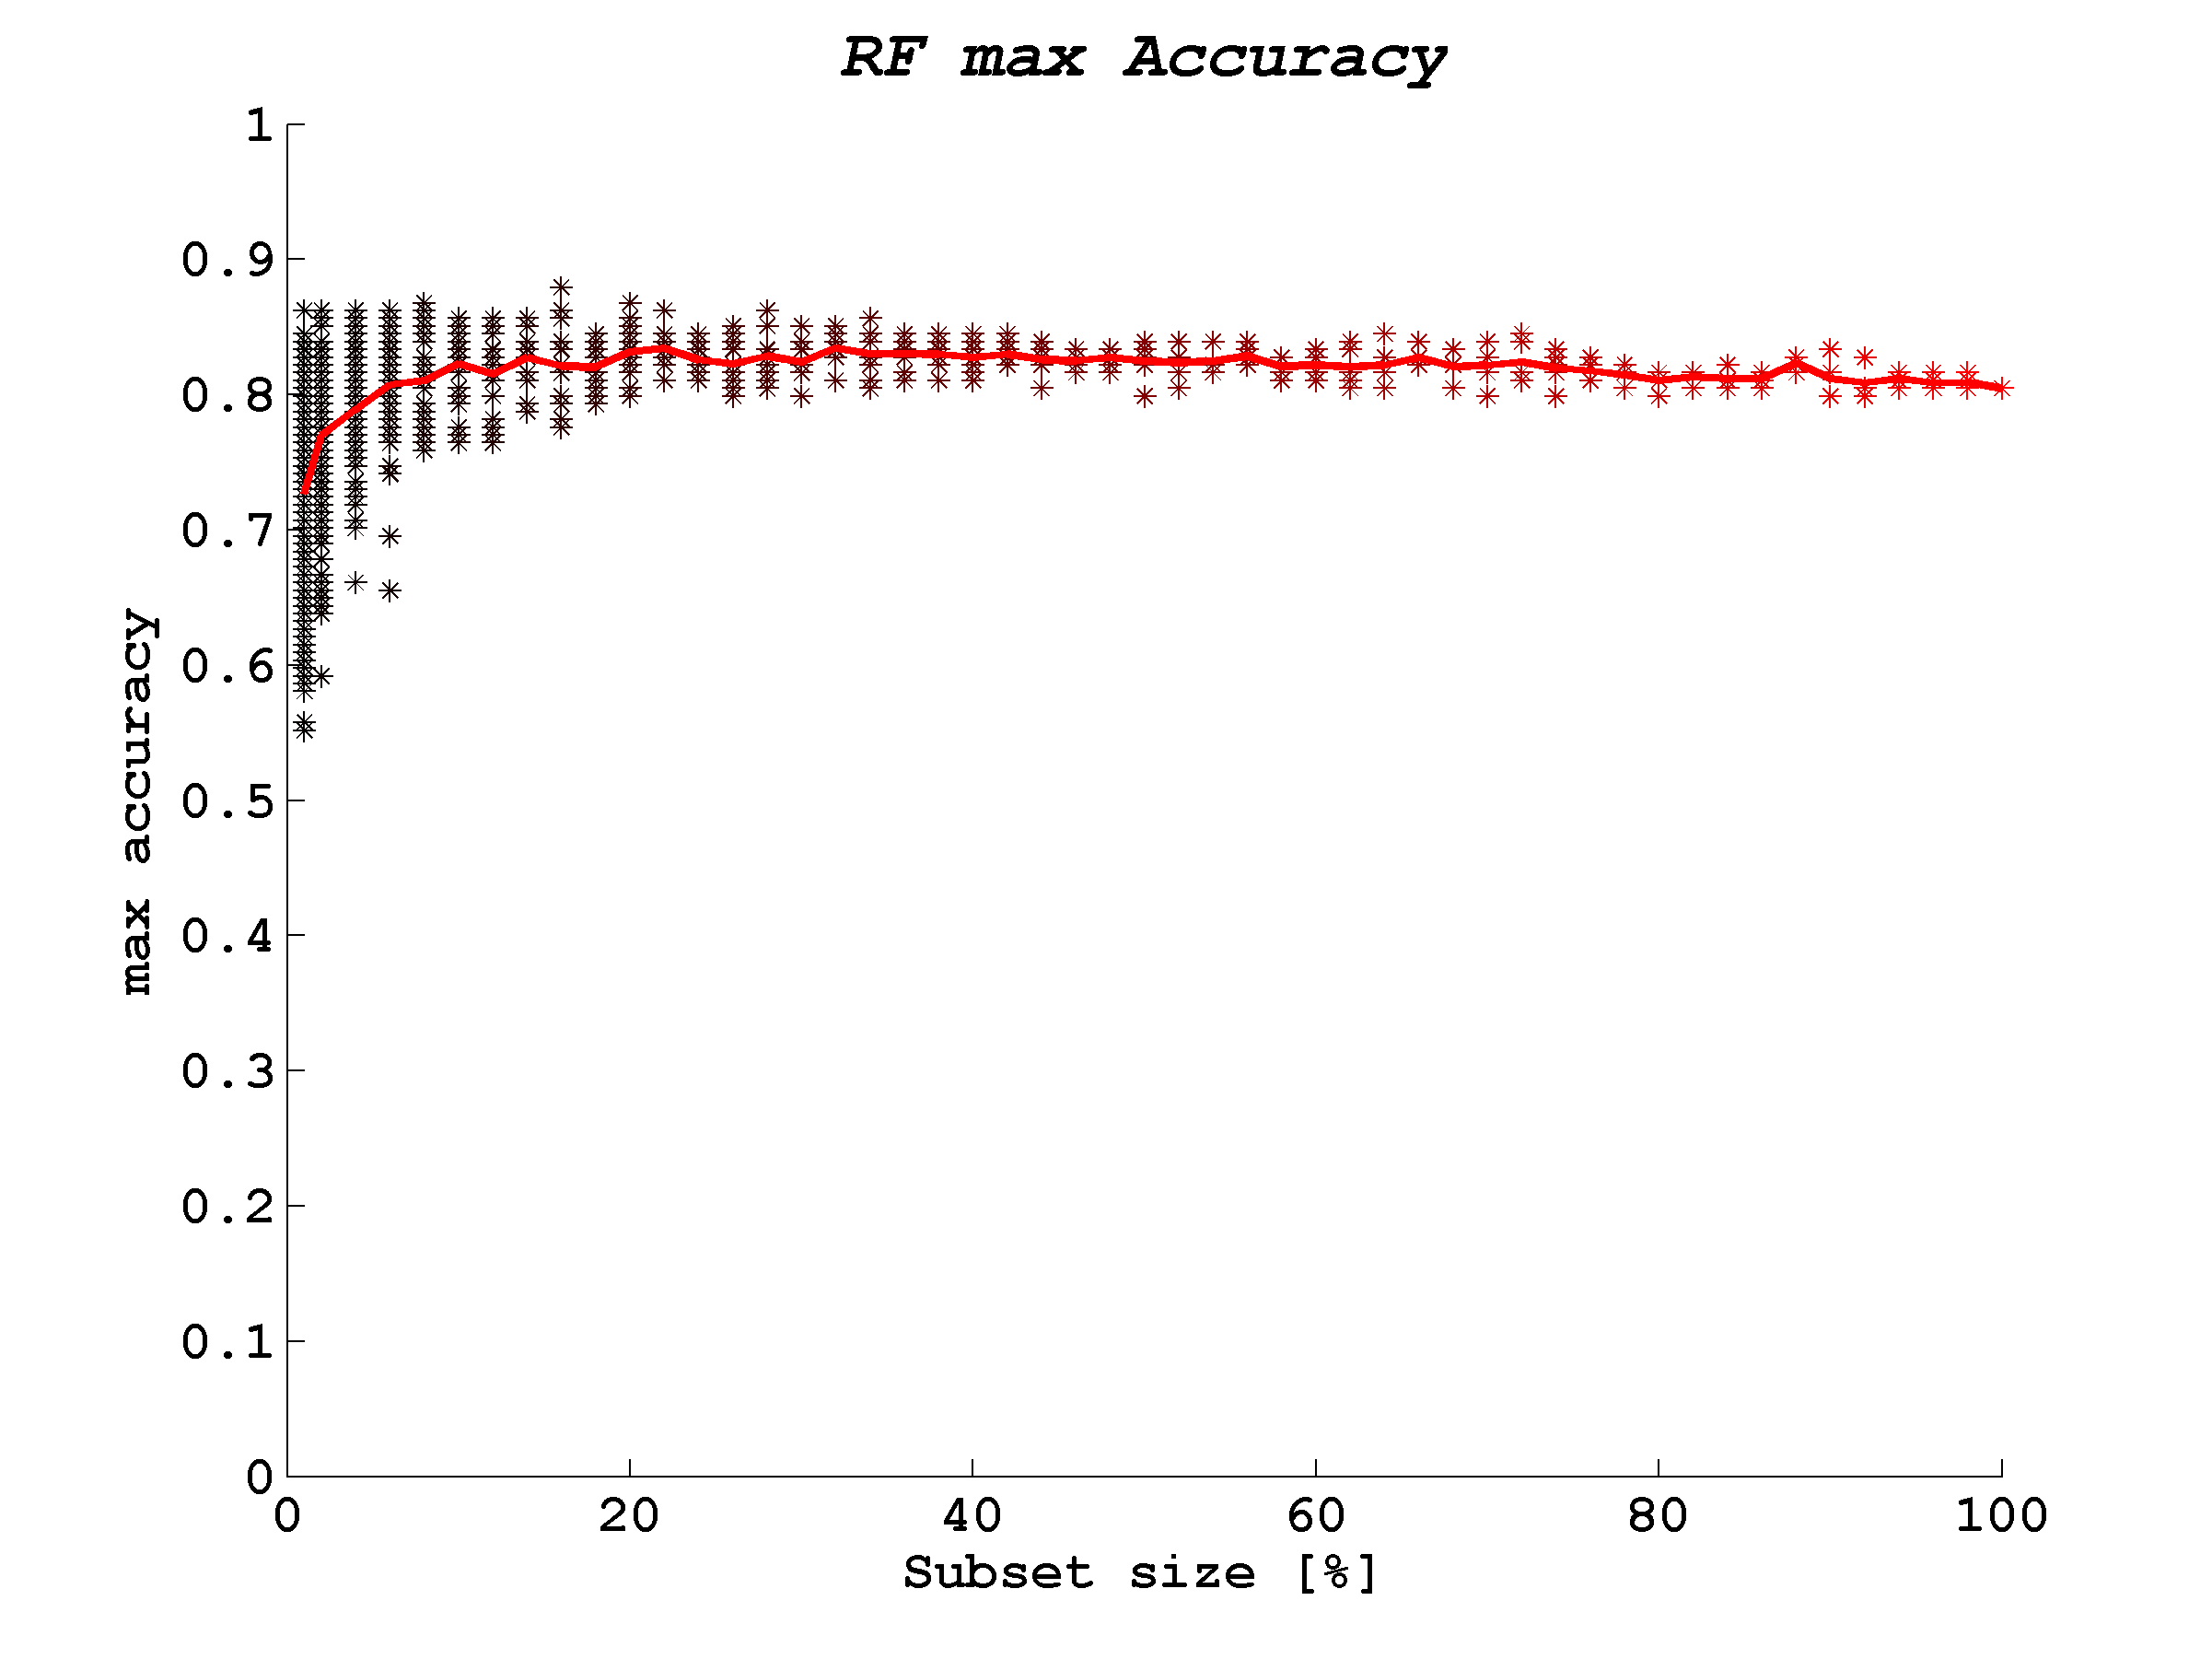
\includegraphics[width=0.75\textwidth]{./images/exp04/MiVHU_RF_acc.png}
      \label{ch6:fig13:b}
    }    
    \caption{Features MiVHU - sample size}
    \label{ch6:fig13}
\end{figure}

The results are similar to the ones shown in Figure \ref{ch6:fig13}. In this case, at $20\%$ of the dataset size a maximum of the \textit{AUC} performance is reached,
even if the negative slope of subsequent data is negligible (see Figure \ref{ch6:fig13:a}).

\vspace{0.5cm}

\subsubsection{Classifier: RF - Features \texttt{MSVHR}}

Figure \ref{ch6:fig14}, shows the results with \texttt{MSVHR} feature set.


\begin{figure}[!htb]
  \centering
    \subfigure[RF MSVHR - AUC]{
      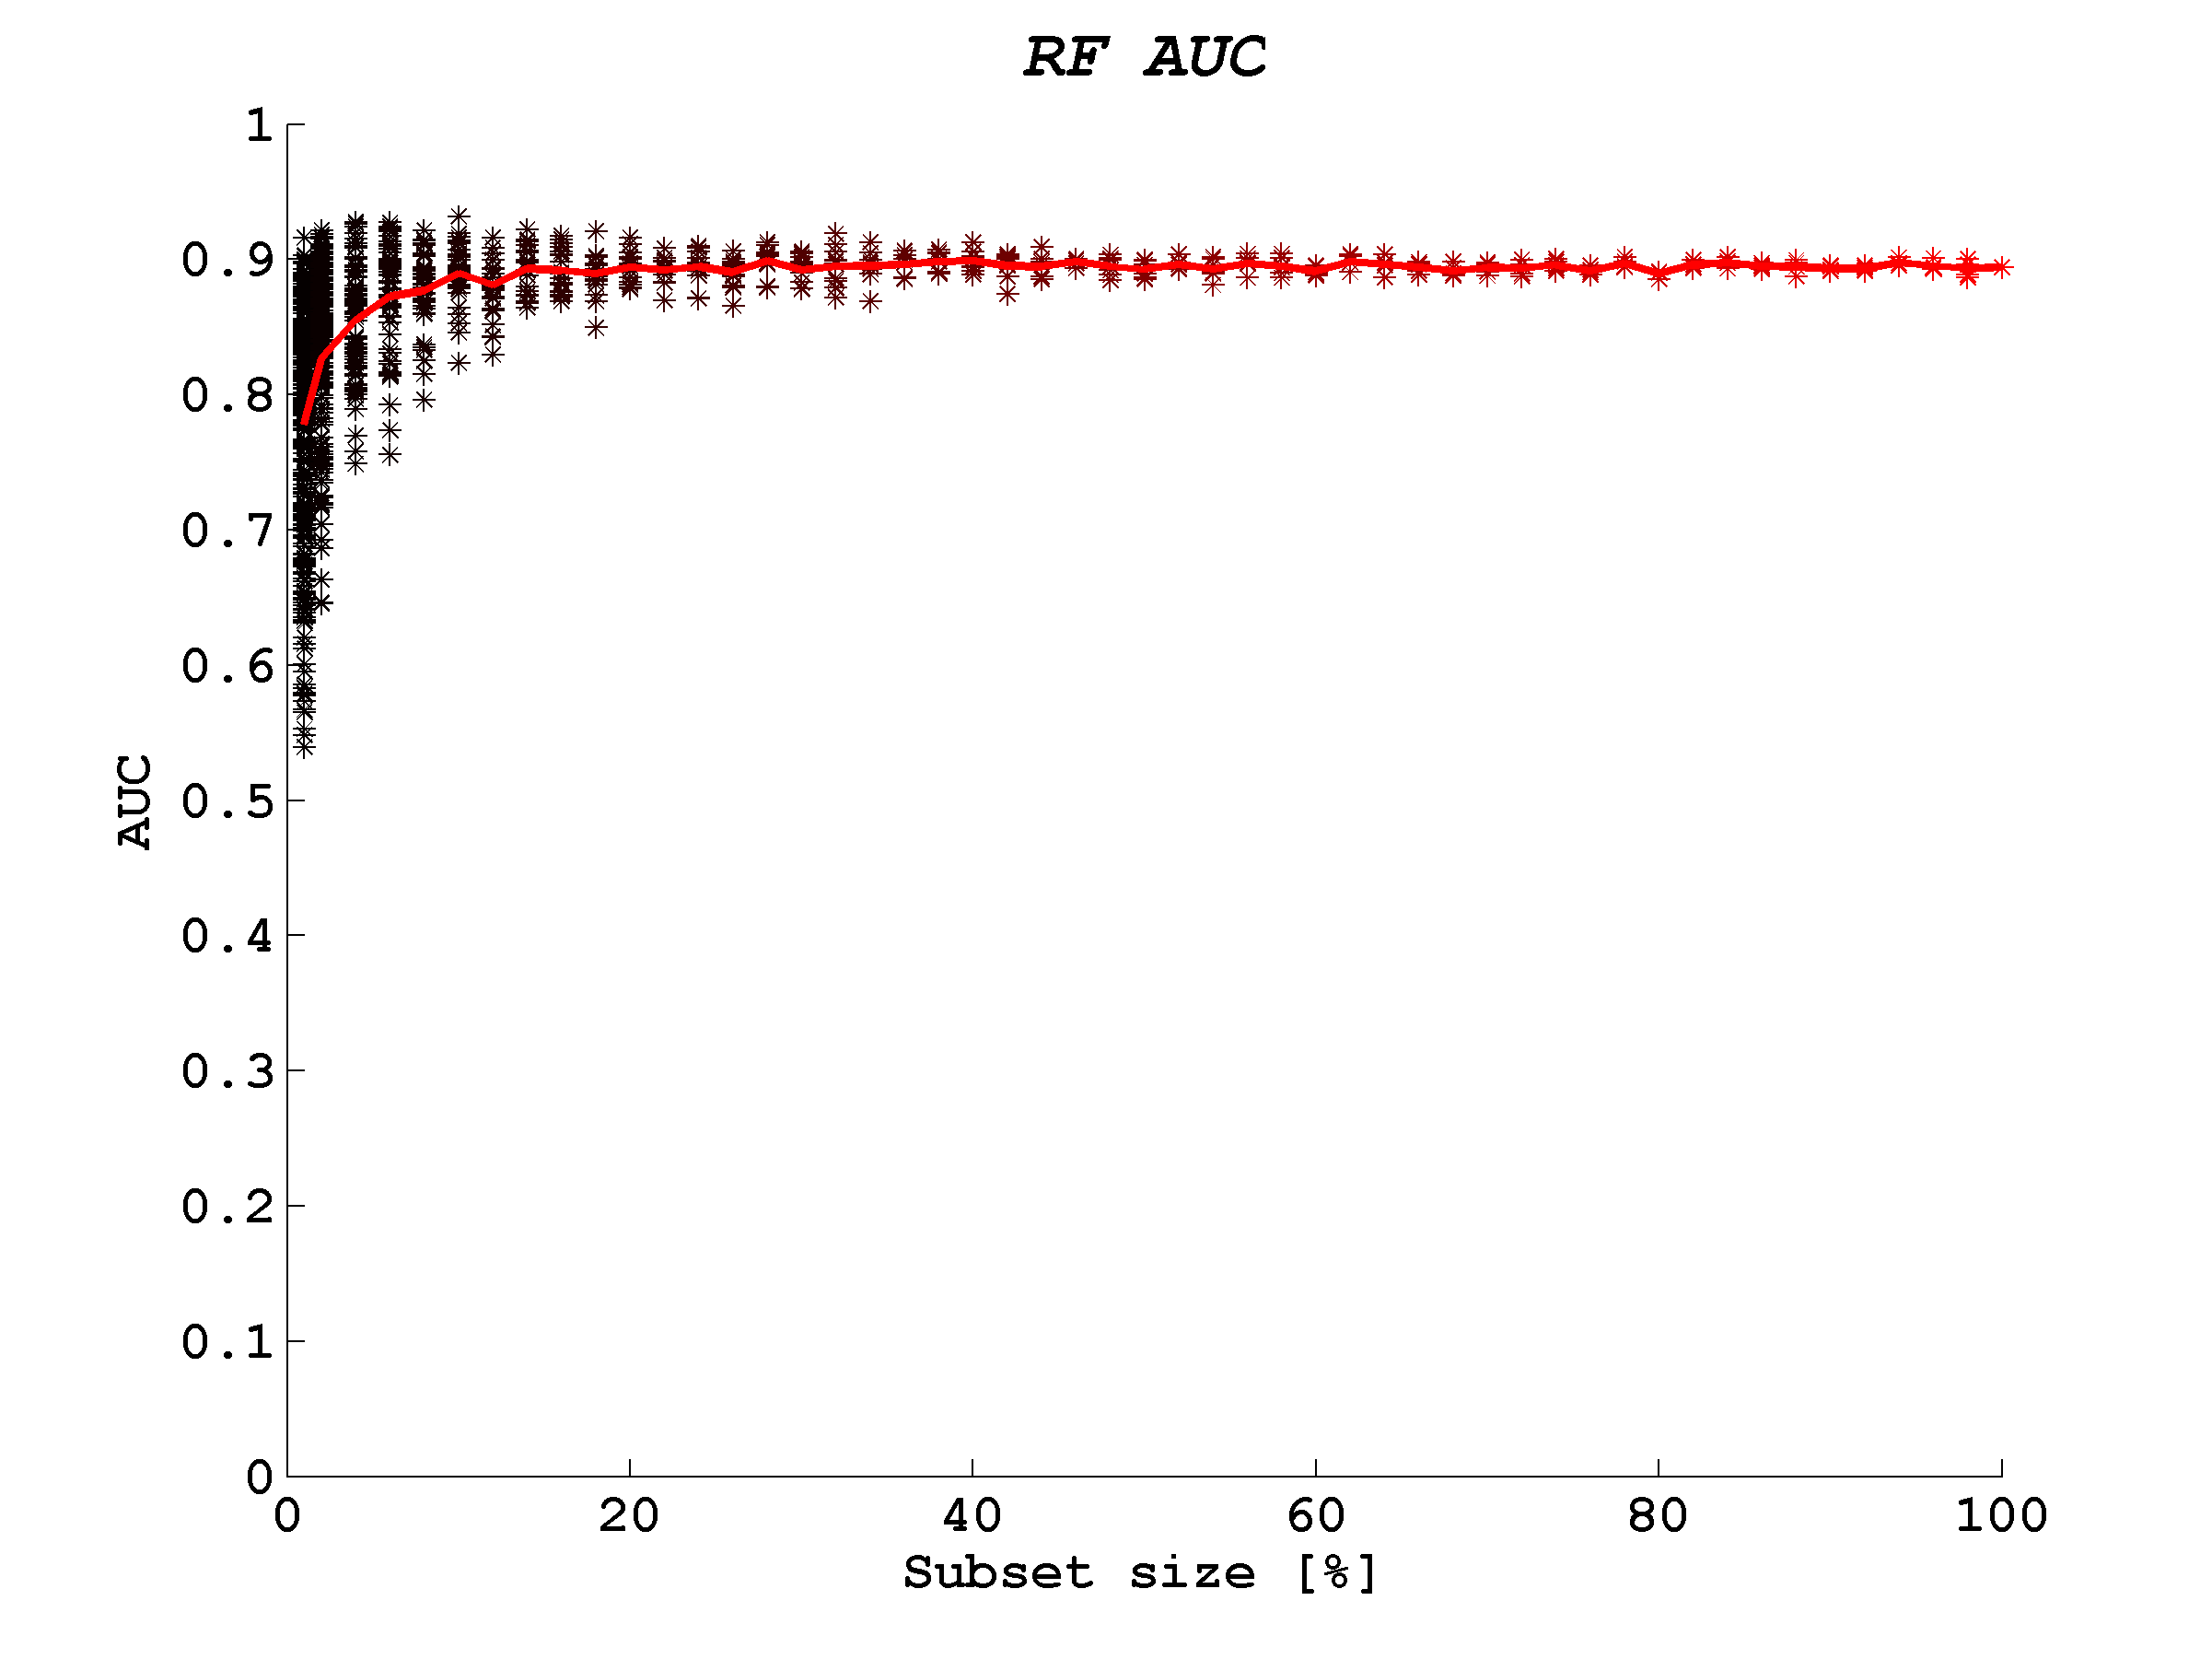
\includegraphics[width=0.75\textwidth]{./images/exp04/MSVHR_RF_AUC.png}
      \label{ch6:fig14:a}
    }
    \\
    \subfigure[RF MSVHR - accuracy]{
      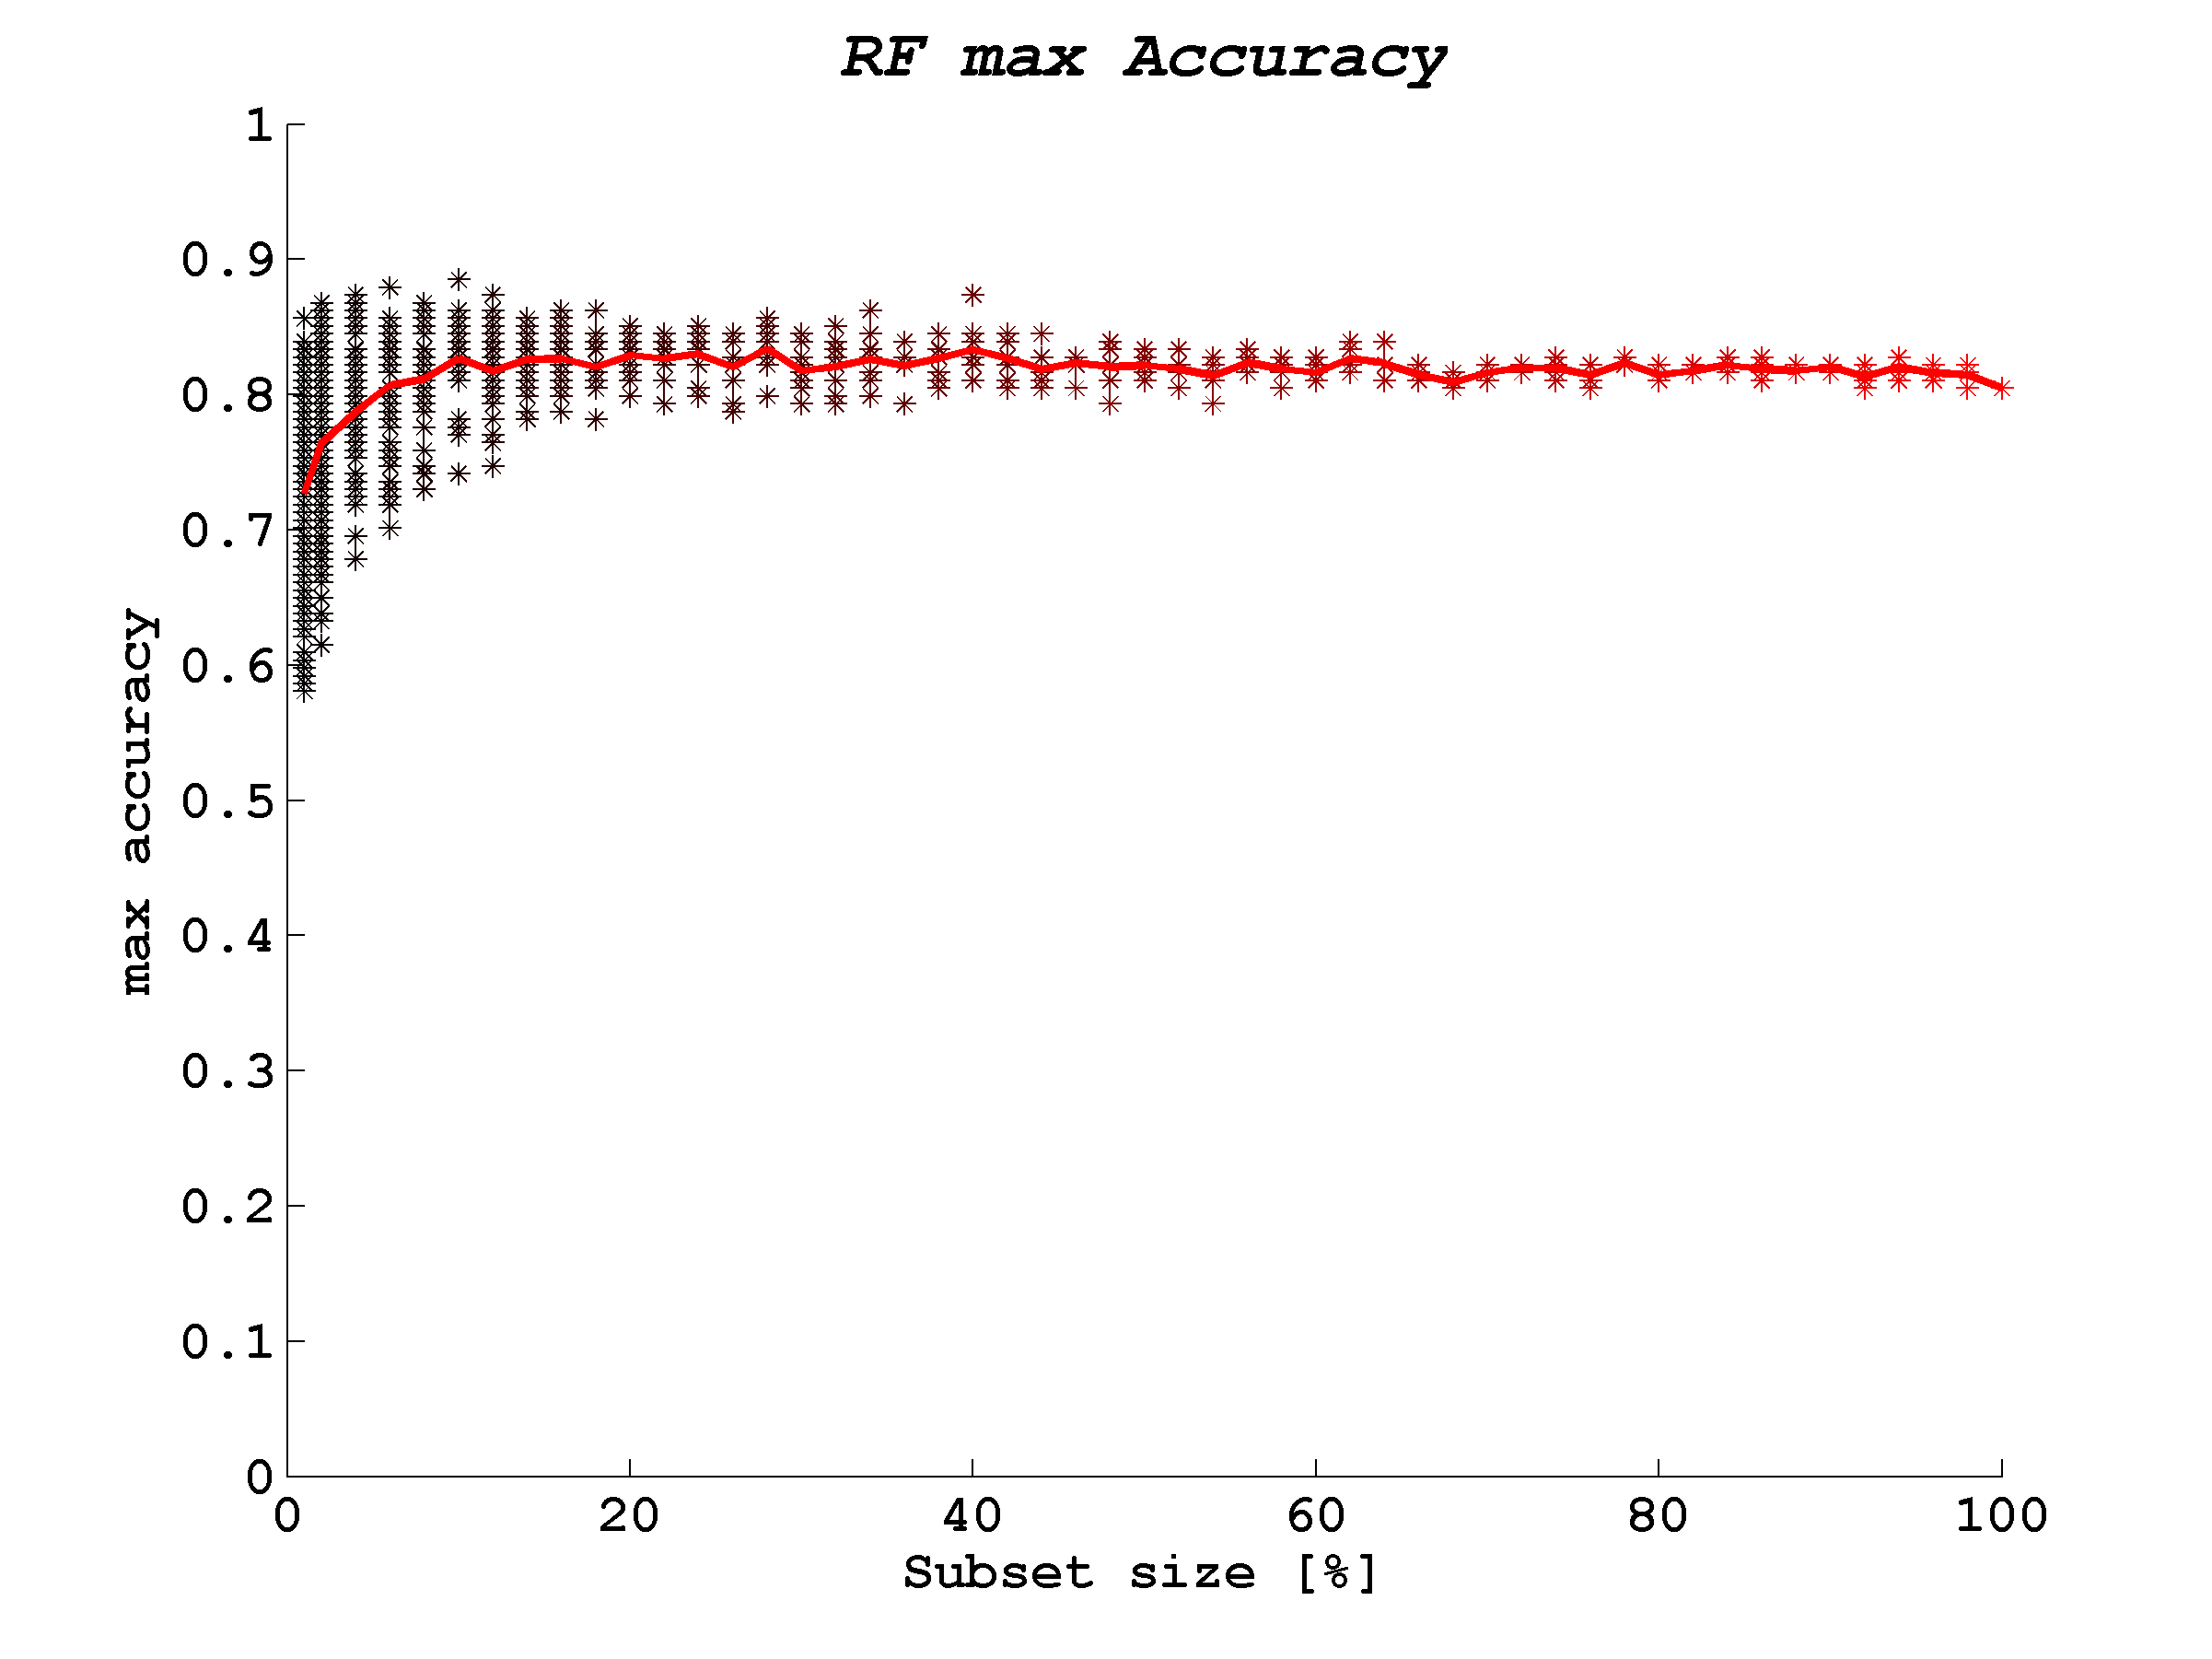
\includegraphics[width=0.75\textwidth]{./images/exp04/MSVHR_RF_acc.png}
      \label{ch6:fig14:b}
    }    
    \caption{Features MSVHR - sample size}
    \label{ch6:fig14}
\end{figure}

The results are similar to the previous ones: in this case the maximum \textit{AUC} performance is reached even at lower subset dimension, and then a steady state 
is maintained, while a negligible variability is reached at about $40\%$ of the dataset (see Figure \ref{ch6:fig14:a}). In this experiment the variability of
\textit{accuracy} appears to be accentuated (see Figure \ref{ch6:fig14:b}).


\vspace{0.5cm}


\subsection{SVM parameters}

In the experiments above we noted that \Glspl{SVM} are more sensible to the selected features and to the size of the dataset, meaning that, in some cases, \Gls{SVM} performs poorly on data.
So we decided to analyze in a deeper way if some of the configuration options of the classifier (i.e. kernel type [Section \ref{ch4:svm}], degree in kernel function, etc. ) could improve the performance.
\\
The Matlab code implemented to run \textit{experiment 5} is listed in \ref{appendixB:exp5}

\vspace{0.5cm}

\subsection{SVM parameters: Experimental results}

We tried different configuration parameters for the \Gls{SVM} classifier on the feature set \texttt{MSiHLV}, of which \Gls{SVM} performed poorly: \textit{AUC} $=0.531$ and
\textit{accuracy} $=0.58$.\\
We changed the allowed parameters in the \textit{libSVM} implementation that we used (see Section \ref{ch4:svm}):

\begin{itemize}
 \item \textit{Kernel type}: \Glspl{RBF} (default) or sigmoidal,
 \item \textit{degree}: from 3 (default) up to 7.
\end{itemize}

As we didn't notice any particular benefit in modifying the parameters above (i.e. the performances remained identical), in the following experiments
we continued using the default parameters. This experiments confirmed that, for our classification problem, \Glspl{RF} turned out to be more robust.


\vspace{0.5cm}


\subsection{Principal Component Analysis}

Even when considering only simple features, the feature space can reach high dimensions (i.e. a lot of components). It is common experience,
in many classification problems, that when the dimensionality increases, the volume of the space increases so fast that the meaningful data become sparse
in a substrate of noise.\\
This situation is often referred to as the \textit{curse of dimensionality} \cite{bellmandynamic}.
In \Gls{ML} problems that involve learning from a finite number of data samples in a high-dimensional feature space,
with each feature having a number of possible values, an enormous amount of training data are required to ensure that there are several samples with each combination of values.
With a fixed number of training samples, the predictive power reduces as the dimensionality increases, and this is known as the \textit{Hughes effect} \cite{hughes}.\\
\Gls{PCA} is a way to reduce the dimensionality of the dataset \cite{PCA_jolliffe}. \Gls{PCA} is a mathematical procedure that uses an orthogonal transformation
(SVD transformation) to convert a set of observations of possibly correlated variables into a set of values of linearly uncorrelated variables called \textit{principal components}.
This transformation is defined in such a way that the components are sorted in descending magnitude of \textit{explained variance}: that is, the first principal component
has the largest possible variance ( accounts for as much of the variability in the data as possible), and each succeeding component, has the highest variance possible under the constraint
that it is orthogonal to (i.e., uncorrelated with) the preceding components. \Gls{PCA} is sensitive to the relative scaling of the original variables, 
and so we applied it on normalized data \cite{PCA02_applications}.
In our experiments we selected some datasets with high dimension feature spaces, applied \Gls{PCA} and classified the resulting components adding one component at a time, with the aim to
observe the classification performances in relation to the number of components and the percentage of explained variance.
\\
The Matlab code implemented to run \textit{experiment 6} is listed in \ref{appendixB:exp6}


\vspace{0.5cm}

\subsection{PCA: Experimental results}

The Matlab function \texttt{pca} returns the principal component coefficients for a data matrix whose rows correspond to observations and columns correspond to variables (i.e. the training feature matrix).
It returns a coefficient matrix. Each column of that matrix contains coefficients for one principal component, and the columns are in descending order of component variance.
By default, \texttt{pca} uses the \Gls{SVD} algorithm. It also returns the percentage of the total variance explained by each principal component.\\
For our analysis we selected two sets of features with many components: \texttt{MSidHLV} (with 148 elements) and \texttt{MSidHUV} (with 292 elements). As in previous experiments,
we used \textit{AUC} and \textit{accuracy} as measures of performance.

\vspace{0.5cm}

\subsubsection{PCA: \texttt{MSidHLV}}

Figure \ref{ch6:fig15} shows the results of \Gls{PCA} applied to \texttt{MSidHLV} feature set. We plotted the results as function of percentage of
explained variance and number of components considered.

\begin{figure}[!htb]
  \centering
    \subfigure[PCA MSidHLV - AUC]{
      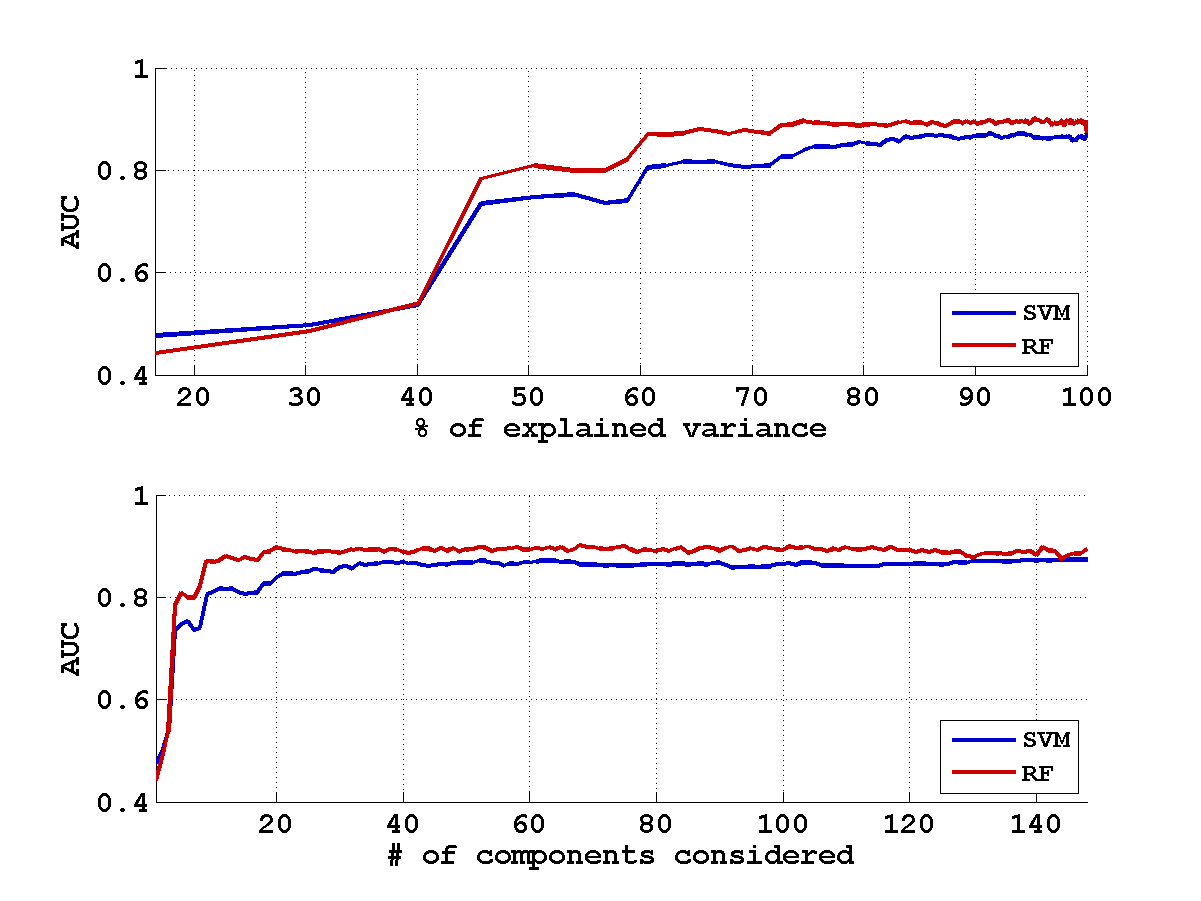
\includegraphics[width=0.75\textwidth]{./images/exp06/pca_AUC_MSidHLV.png}
      \label{ch6:fig15:a}
    }
    \\
    \subfigure[PCA MSidHLV - accuracy]{
      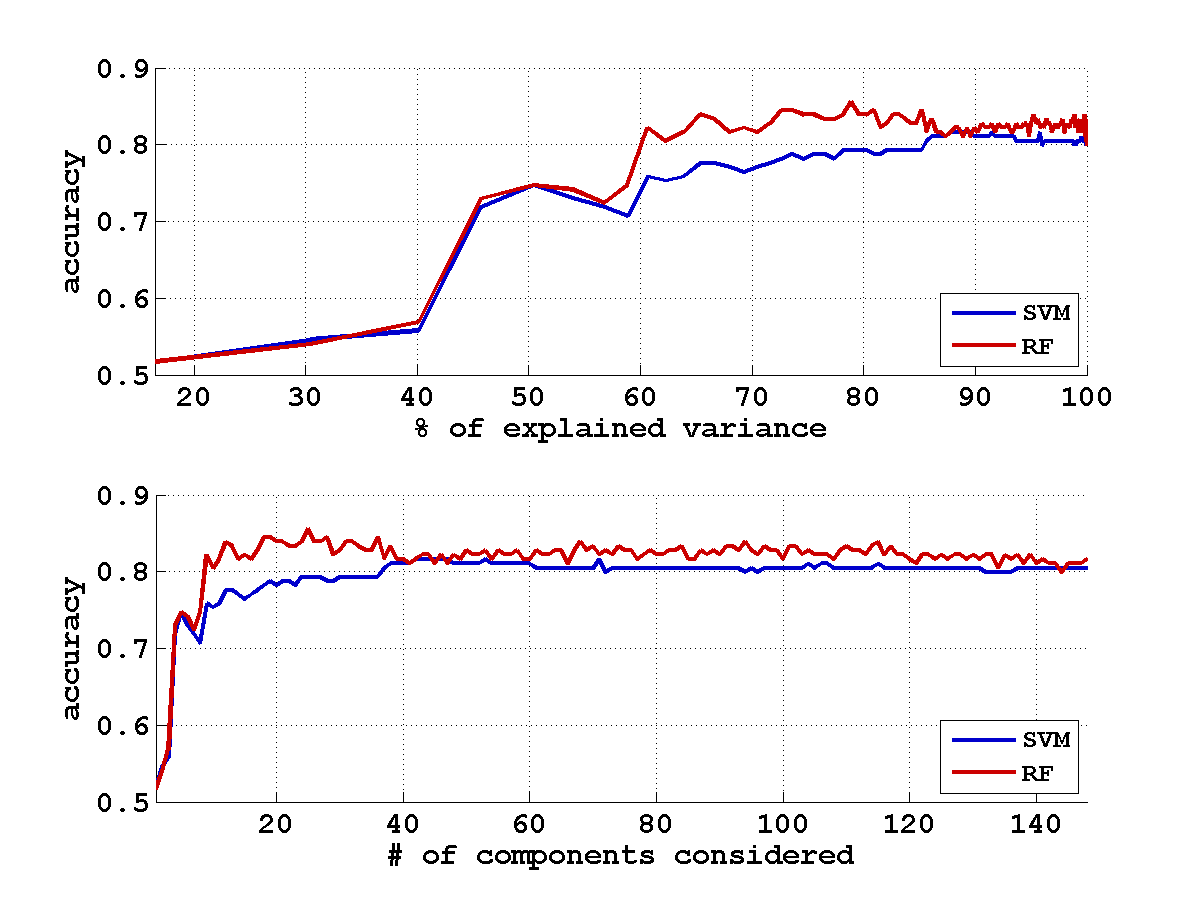
\includegraphics[width=0.75\textwidth]{./images/exp06/pca_acc_MSidHLV.png}
      \label{ch6:fig15:b}
    }    
    \caption{Features MSidHLV - Principal Component Analysis}
    \label{ch6:fig15}
\end{figure}

The results show a generally better performance of \Gls{RF} than \Gls{SVM}. In terms of \textit{AUC} (see Figure \ref{ch6:fig15:a}), the \Gls{RF} classification reaches
a maximum at about $74\%$ of explained variance (20 components), and then it remains almost stable with small fluctuations due to noise.
The \Gls{SVM} classification shows similar behavior.\\
In terms of \textit{accuracy} (see Figure \ref{ch6:fig15:b}) the \Gls{RF} classification reaches a maximum at about $79\%$ of explained variance (27 components)
and then starts decreasing moderately. \Gls{SVM} shows a maximum at about $80\%$ (43 components): the overall behavior appears to be steadier.

\vspace{0.5cm}


\subsubsection{PCA: \texttt{MSidHUV}}

Figure \ref{ch6:fig16} shows the results of \Gls{PCA} applied to \texttt{MSidHUV} feature set. Also in this case, we plotted the results as function of percentage of
explained variance and number of components considered.

\begin{figure}[!htb]
  \centering
    \subfigure[PCA MSidHUV - AUC]{
      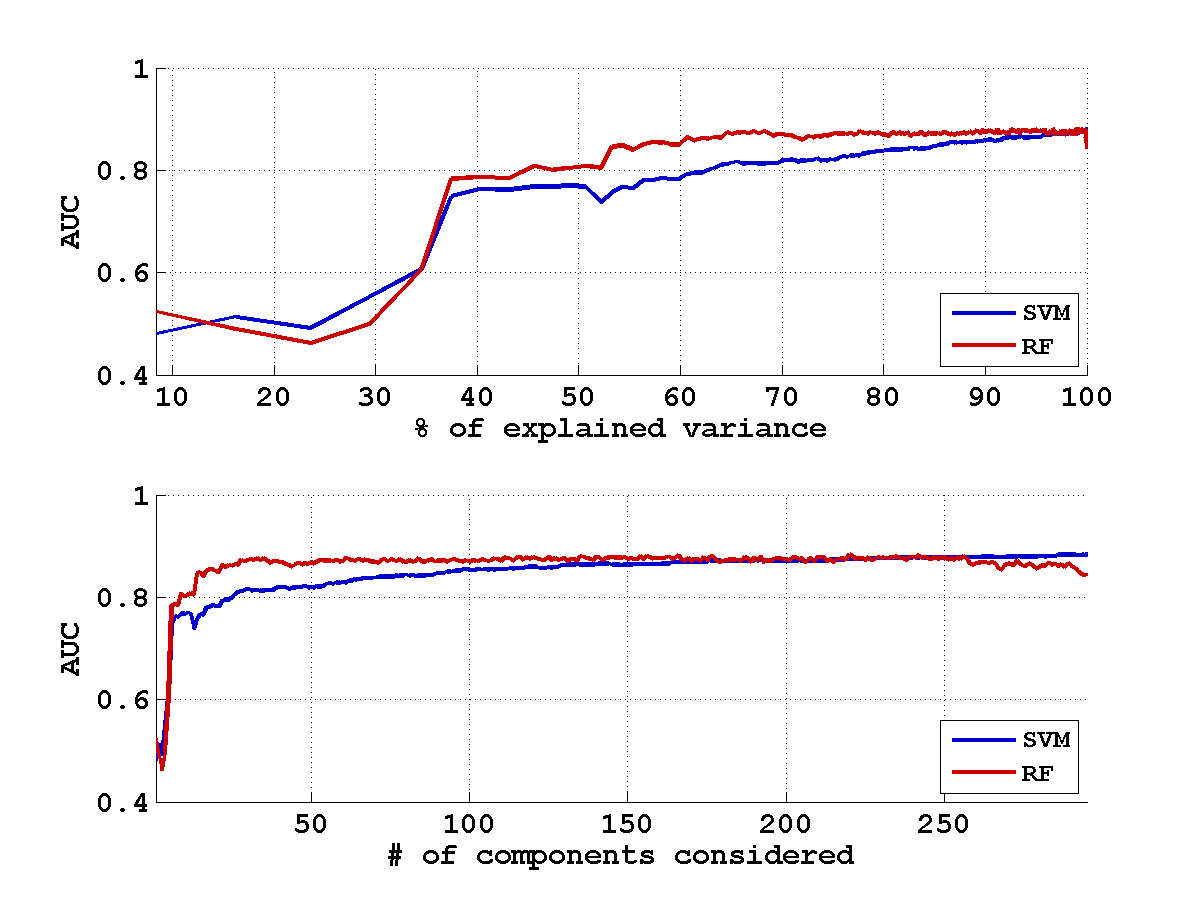
\includegraphics[width=0.75\textwidth]{./images/exp06/pca_AUC_MSidHUV.png}
      \label{ch6:fig16:a}
    }
    \\
    \subfigure[PCA MSidULV - accuracy]{
      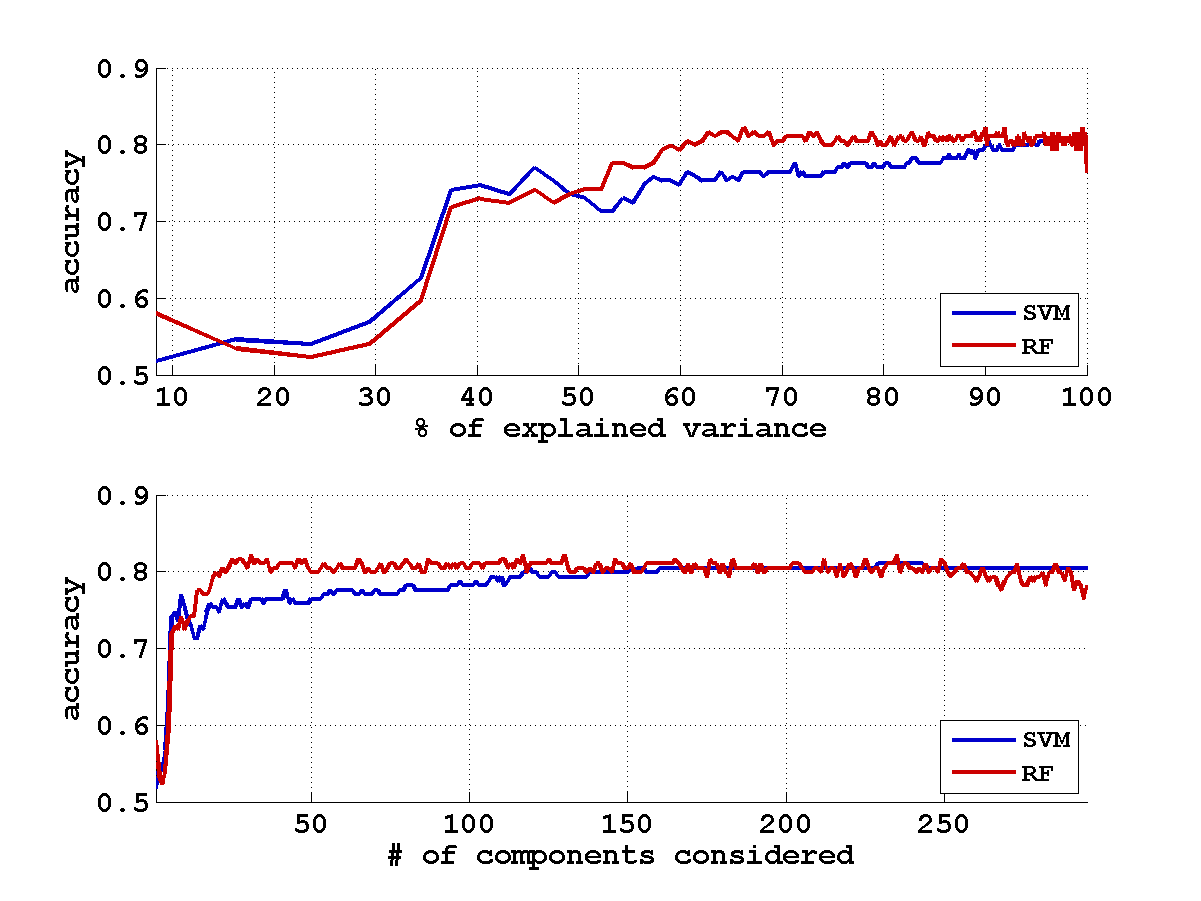
\includegraphics[width=0.75\textwidth]{./images/exp06/pca_acc_MSidHUV.png}
      \label{ch6:fig16:b}
    }    
    \caption{Features MSidHUV - Principal Component Analysis}
    \label{ch6:fig16}
\end{figure}


The results show a generally better performance of \Gls{RF} than \Gls{SVM}, even if, at high number of components ($>250$), \Gls{SVM} still find information useful
fpr classification and improves performance, while \Gls{RF} starts decreasing. It appears that, with a high number of components, \Gls{RF} becomes more sensible
and the performance becomes more noisy.
In terms of \textit{AUC} (see Figure \ref{ch6:fig16:a}), the \Gls{RF} classification reaches
a maximum at about $69\%$ of explained variance (33 components), and then it decreases with fluctuations due to noise induced by further components.
The \Gls{SVM} classification appears more stable and contiunes increasing.\\
In terms of \textit{accuracy} (see Figure \ref{ch6:fig16:b}) the \Gls{RF} classification reaches a maximum at about $66\%$ of explained variance (26 components)
and then starts decreasing. \Gls{SVM} shows a local maximum at about $45\%$ (just 12 components) and then has an important dagradation of performance up to 
about $54\%$ of explained variance. Then it starts increasing again up to the end.


\vspace{0.5cm}

\subsection{Size of the Image Patch}

In all the experiments above, we considered the size of each image patch, on which to compute features, to be $100\times100$ pixels.
We wanted to analyze if there is a smaller sub-image that includes all the meaningful information, while the boundary contains essentially background (i.e. noise for the
purposes of classification), while an excessively small patch would not allow to classify data.\\
So we run experiments considering, form time to time, bigger portions of the images and analyzed the classification performances.
\\
The Matlab code implemented to run \textit{experiment 7} is listed in \ref{appendixB:exp7}



\vspace{0.5cm}

\subsection{Image Size: Experimental Results}

We tried different image sizes, starting from 10px up to 100px, with a step of 10px. We calculated different feature sets on the images and finally we performed classifications.
Even if it appeared to be quite hard to find a \textquotedblleft{}best image size\textquotedblright, we could draw some considerations about the relation among image size and
some of the features selected.\\
Here we report the most interesting ones, focusing in particular on the following features:

\vbox{
\begin{itemize}
 \item Color Histograms (H),
 \item LBP$^{riu2}$ (L),
 \item VAR (V).
\end{itemize}
}
In this case we used \textit{AUC} as a measure of performance. 

\vspace{0.5cm}


\subsubsection{Image Size: SVM Classifier}

By ordering the \Gls{SVM} classification results in ascending order for cumulate \textit{AUC} along feature size, we could plot the behavior as reported in Figure \ref{ch6:fig17} and
in Figure \ref{ch6:fig18}

\begin{figure}[!hbf]
 \begin{center}
  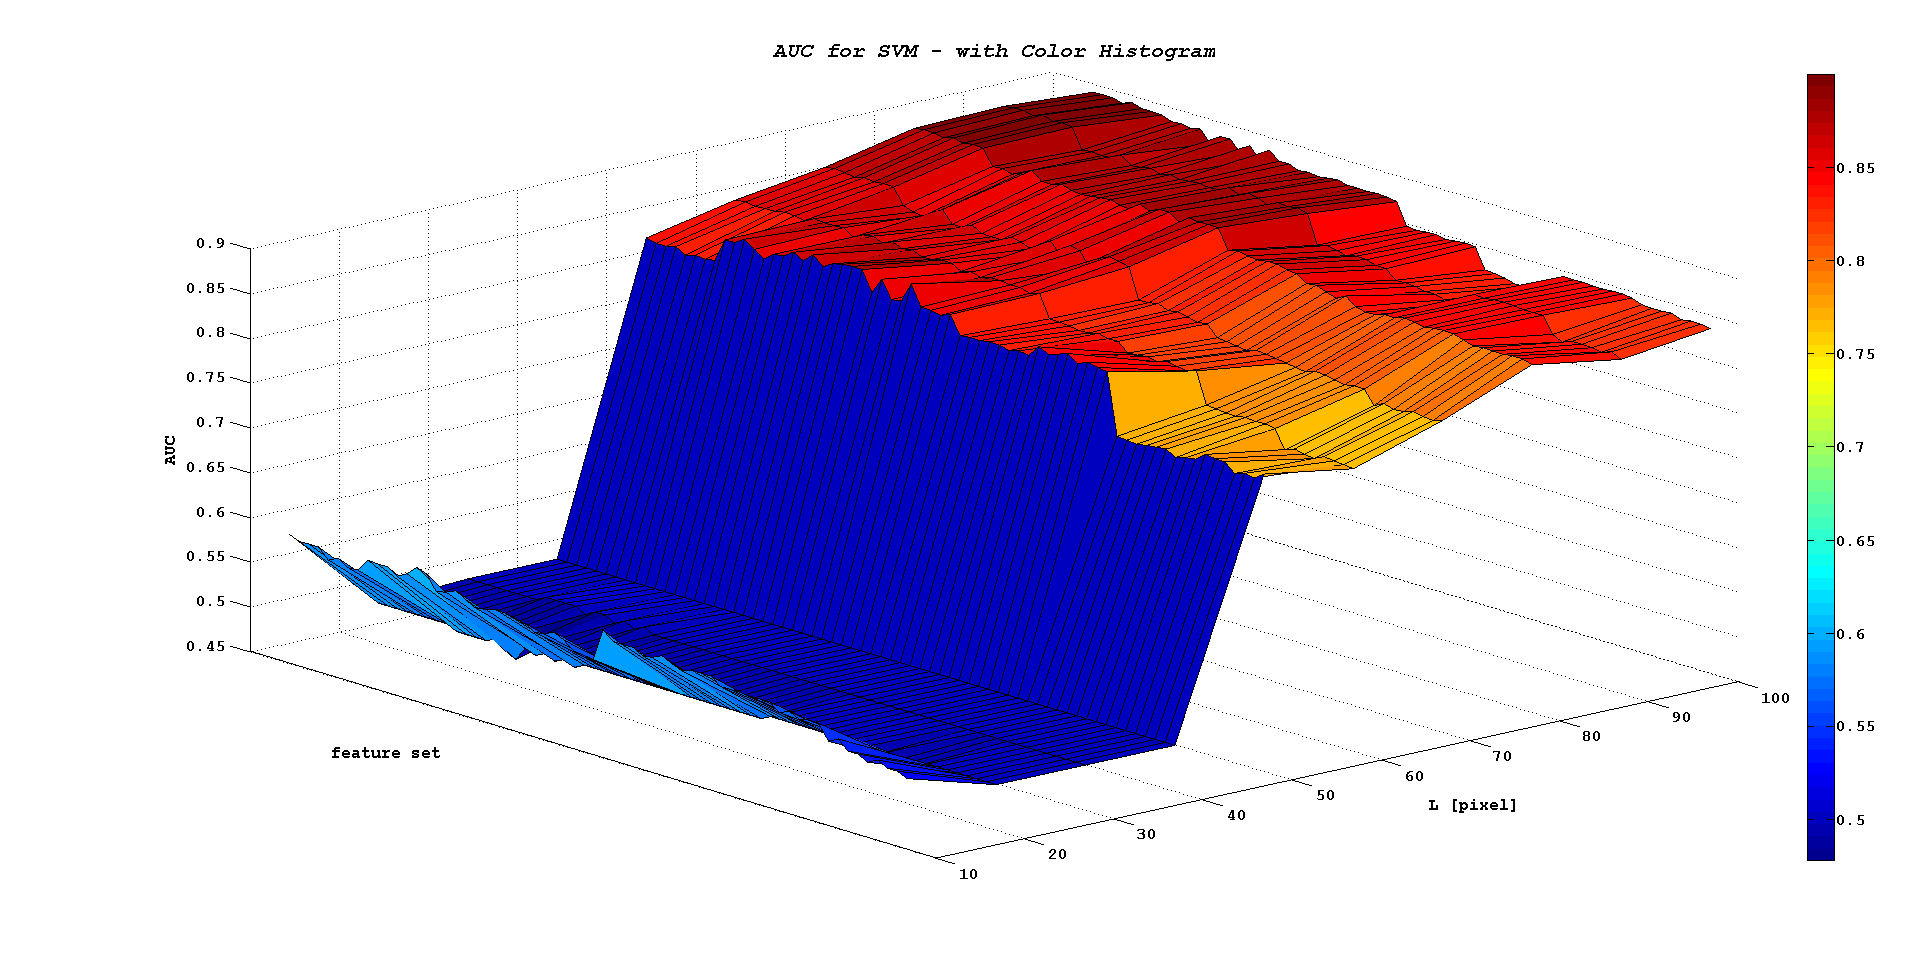
\includegraphics[width=0.92\textwidth]{./images/exp07/SVM_AUC_H.png}
  \caption{Image size and sets with 'H' feature - SVM classifier}
  \label{ch6:fig17}
 \end{center}
\end{figure}

Ordering the results we found that \textbf{all} the feature sets with the \texttt{H} elements have the same behavior.
Figure \ref{ch6:fig17} shows that \Gls{SVM} is unable to classify any dataset containing the \texttt{H} feature up to image size of 40px. Please note that
an \textit{AUC} of $0.5$ means \textquotedblleft{}random classification\textquotedblright. After 50px the performance increases abruptly to high values.


\begin{figure}[!hbf]
 \begin{center}
  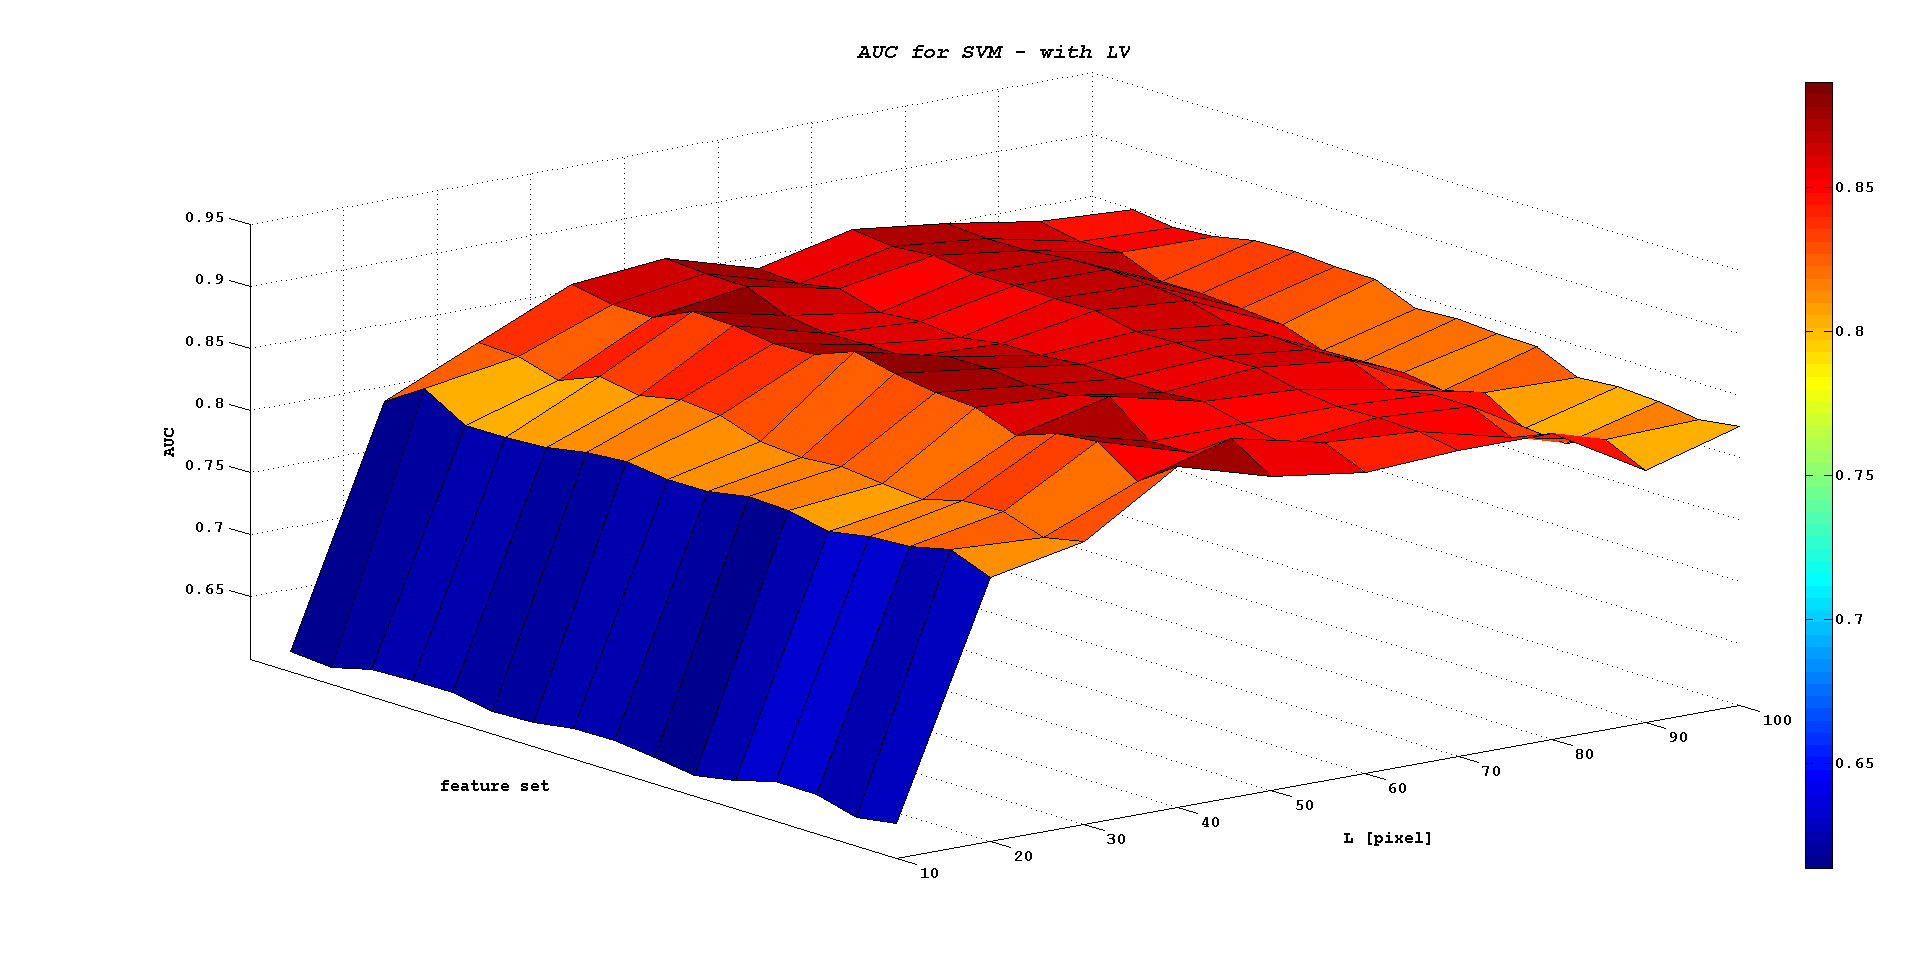
\includegraphics[width=0.92\textwidth]{./images/exp07/SVM_AUC_LV.png}
  \caption{Image size and sets with 'LV' features - SVM classifier}
  \label{ch6:fig18}
 \end{center}
\end{figure}

Among the other feature set (i.e. the ones not containing \texttt{H}), it emerged that the ones containing the \texttt{LV} combination have the best performance.
Figure \ref{ch6:fig18} shows that those sets have a maximum generally at about 40px. With higher image size the performance slightly decreases.


\vspace{0.5cm}


\subsubsection{Image Size: RF Classifier}

We performed the same operations on the results coming from our \Gls{RF} classifier and found similar results. In this case, ordering in ascending order 
the result for mean performance over image size, we found that \textbf{all} the feature set containing the \texttt{HLV} components showed good results and
also performed in the same way (see Figure \ref{ch6:fig19}).

\begin{figure}[!hbf]
 \begin{center}
  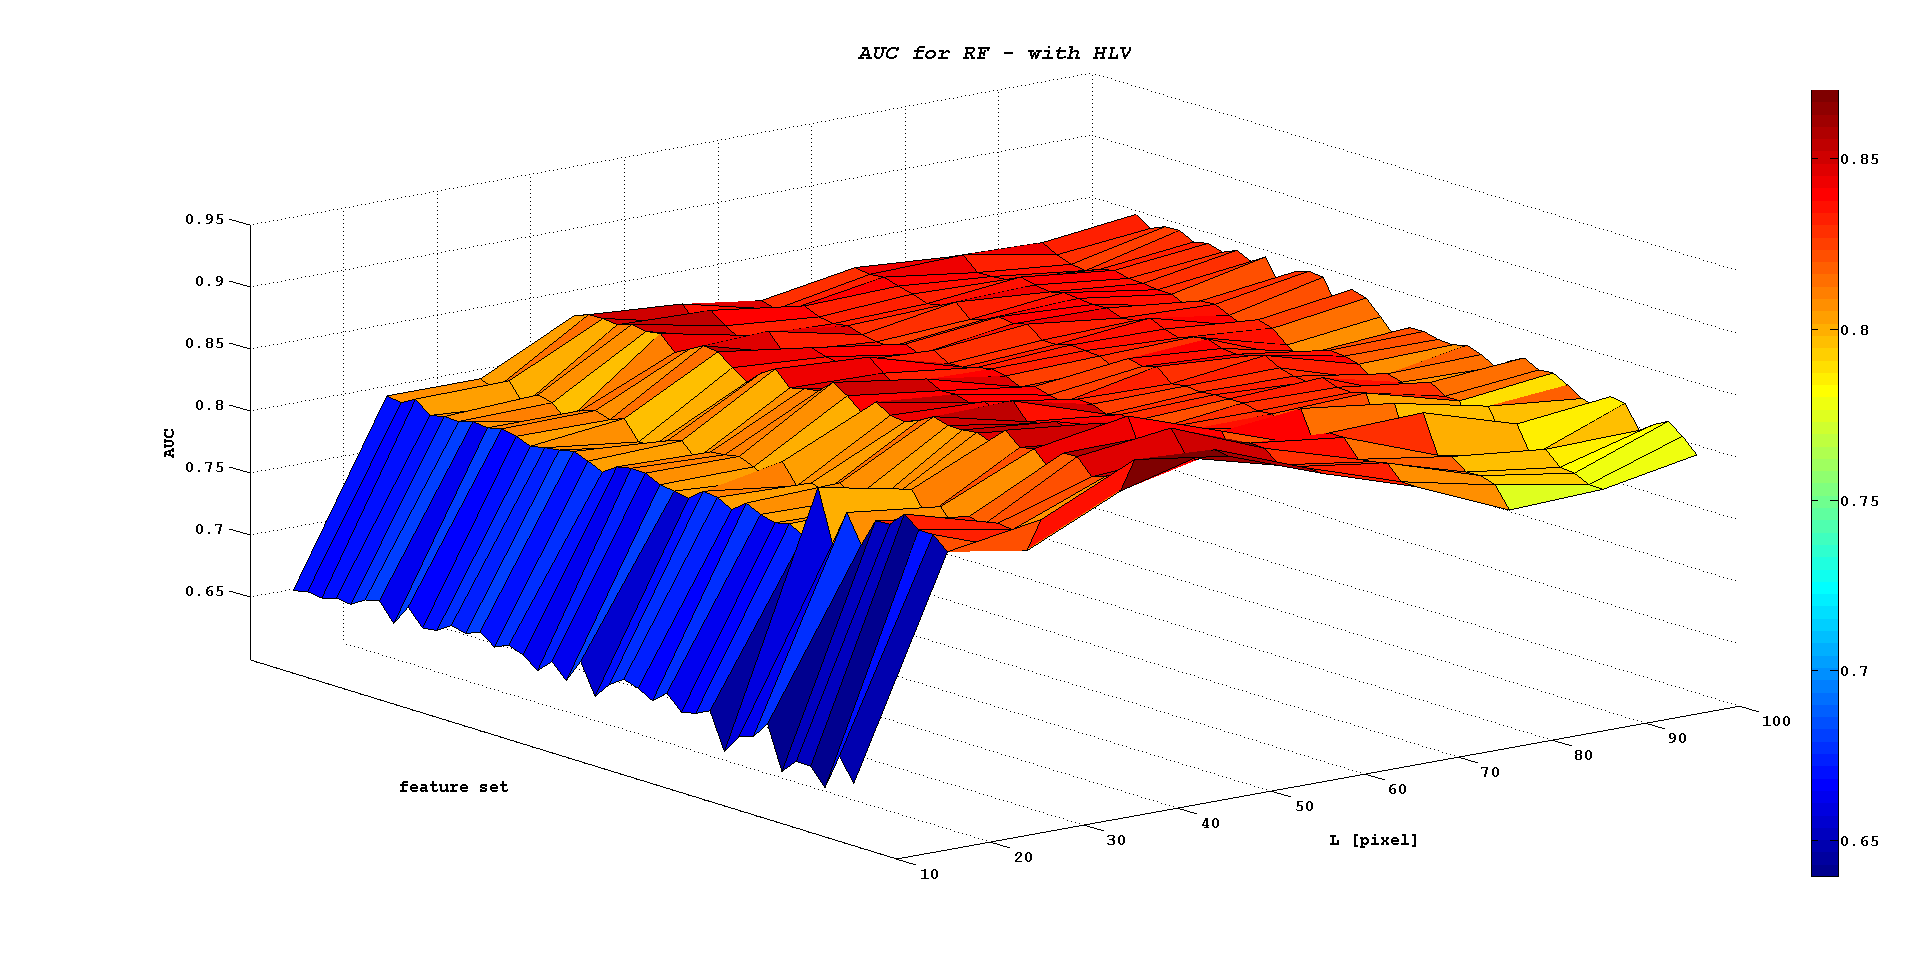
\includegraphics[width=0.92\textwidth]{./images/exp07/RF_AUC_HLV.png}
  \caption{Image size and sets with 'HLV' features - RF classifier}
  \label{ch6:fig19}
 \end{center}
\end{figure}

Figure \ref{ch6:fig19}, similarly to Figure \ref{ch6:fig18}, shows a general maximum at about 40px.


\vspace{0.5cm}


\section{Accuracy of Humans}

In this section we illustrate the performances of the users of the website described in Chapter \ref{chapter5}.
We gathered data from a total of 45 test subjects, 8 of which have expertise in biology (i.e. may have some prior expectations or experience on a mitosis’ appearance),
and none of which routinely works with histology datasets. No subject was allowed to take the test twice. In total, subjects provided 3009 classifications
(on average 67 per subjects), resulting in an average of 17.3 classifications for each of the 174 evaluation samples.
Each subjects dedicated an average of 49 minutes to the test.
Below, we compare the performance of such subjects to the 7 top-performing algorithms in the 2012 ICPR mitosis detection contest, all of which were learned
on the training images of the MITOS dataset. For a given algorithm, a \textbf{C1} evaluation sample is considered a true positive if and only if, in the corresponding
image of the MITOS dataset, the algorithm detected a mitosis whose centroid is within 8 $\mu$m (20 px) from the coordinates given by the algorithm;
else, the sample is considered a false positive (this is the same criterion used for evaluation of the ICPR contest).
A \textbf{C0} evaluation sample is a true negative if and only if the algorithm
returned no detections in a range of 16 $\mu$m (40 px), else it is a false negative.\\
Note that the results reported below for algorithms do not directly map
to the results of the ICPR contest (shown in Section \ref{ch3:icpr_perf}). In fact, we are computing the algorithms’
performance in a classification task on a balanced dataset, whereas the algorithms’ parameters (such as thresholds) were optimized for solving a detection
task where the prevalence of mitosis over non-mitosis was much lower. Therefore, we can expect that the reported performance for each algorithm is a lower
bound of the performance it could obtain when properly tuned for this task.
For this same reason, the results below should not be used to compare different algorithms with each other.
We also compare the performances of the users with best classifications obtained in Chapter \ref{chapter4}, which instead is designed on the same problem
as the one presented to the users.


\clearpage
%\vspace{0.5cm}

\subsection{Humans and ICPR Contest Algorithms}

For a given set of N classifications produced by an human or algorithm, the accuracy is defined as the fraction of classifications which are 
correct\footnote{for all algorithms, N = 174 since we computed an output for each evaluation sample;
instead, test subjects were not required to evaluate all samples}.
Because our evaluation set has the same prevalence of both classes, a random classifier has an expected accuracy = 0.5. Subjects could assign each sample to one of
four probability values: for each user, we computed the accuracy when using all three meaningful thresholds ($p(C1) = {0.1, 0.5, 0.9}$), and selected the maximum
resulting accuracy value.\\

\begin{figure}[!htb]
   \begin{center}
    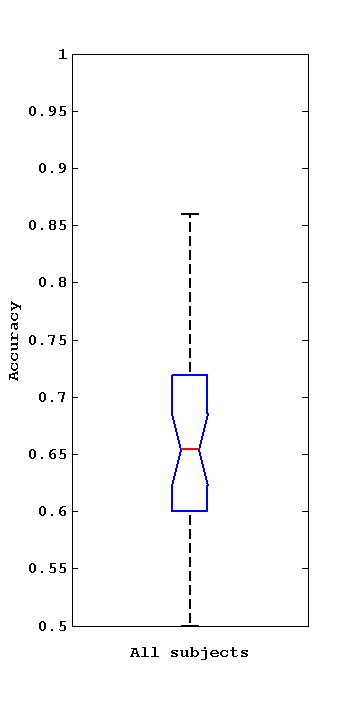
\includegraphics[width=0.28\textwidth]{./images/human/p11.png}
    \caption{Accuracy distribution of humans}
    \label{ch6:fig20}
    \end{center}
\end{figure}


Figure \ref{ch6:fig20} reports the accuracy distribution for all test subjects, while Figure \ref{ch6:fig21} shows the
performance of the 5 best test subjects (\ref{ch6:fig21:a}), compared with the performance
of the 7 algorithms (\ref{ch6:fig21:a}). The average classification accuracy for users is 0.661,
comparable with the accuracy of the worst of the considered algorithms; The best
individual yielded an accuracy of $0.859 \pm 0.012$, which is close to the accuracy
of the second-scoring algorithm, and worse $(p < 0.01)$ than the most accurate
algorithm (accuracy = $0.873 \pm 0.004$).


\begin{figure}[!htb]
  \centering
    \subfigure[]{
      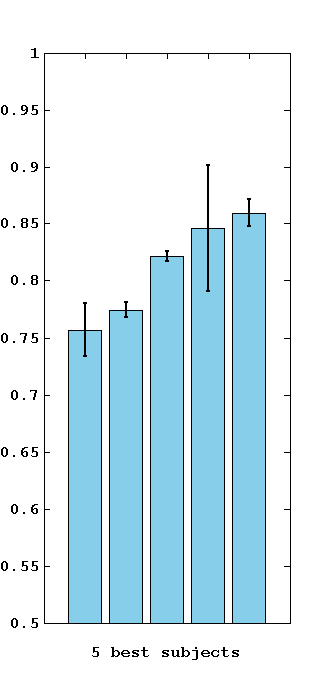
\includegraphics[width=0.351\textwidth]{./images/human/p12.png}
      \label{ch6:fig21:a}
    }
    \hspace{1mm}
    \subfigure[]{
      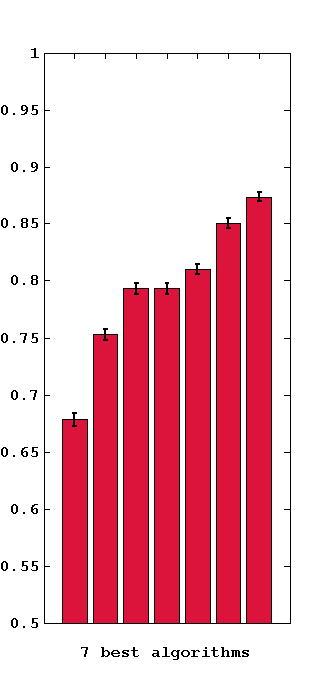
\includegraphics[width=0.351\textwidth]{./images/human/p13.png}
      \label{ch6:fig21:b}
    }
    \caption{best Humans' performance vs. ICPR algorithms}
    \label{ch6:fig21}
\end{figure}

All users with $N \geq 10$ performed better than chance; most achieved an
accuracy between 0.60 and 0.75. Only three users (one of which with significant experience in cytology but not in this specific problem)
exceeded an accuracy of 0.80. Differences in human performance are partly explained by different
amounts of motivation end effort put in the test; still, we observed that many
users who dedicated a significant amount of time and effort to study the training set and complete the test obtained a performance close to the average.
Most users described the problem as \textquotedblleft{}very difficult\textquotedblright”.\\
Some users gave indications about the evaluation criteria which they devised during classification. Most of them focused on the shape of the dark element in the middle.
Mitotic samples where mostly the one with blurry or bumpy edges, while non-mitotic samples where the ones with a smooth shape.
Most of them ignored the surrounding area.\\
Figure \ref{ch6:fig22} reports the performance of test subjects and algorithms in \Gls{ROC} space. IDSIA and Utrecht institutions provided confidence values for each classification,
from which \Gls{ROC} curves were computed.

\begin{figure}[!htb]
   \begin{center}
    \includegraphics[width=0.94\textwidth]{./images/human/p2.png}
    \caption[ROC plot humans vs. algorithms]{For each subject 3 points are reported, corresponding to the three possible thresholds.
    Full ROC curves could be plotted for IDSIA (thick blue) and Utrecht (thin blue),who provided soft confidence values for each detection.}
    \label{ch6:fig22}
    \end{center}
\end{figure}

\vspace{0.5cm}

\subsection{Humans and ad hoc Classifiers}

In this section we compare the performances of users with the classifiers that we trained on the same problem. In particular we selected two of the best performing classifiers with 
reference to Tables \ref{ch6:tab9} and \ref{ch6:tab11}.

\begin{figure}[!htb]
   \begin{center}
    \includegraphics[width=0.94\textwidth]{./images/human/class_humans.png}
    \caption[ROC plot humans vs. classifiers]{For each subject 3 points are reported, corresponding to the three possible thresholds.
    Full ROC curves are shown for two best feature-sets for SVM and RF}
    \label{ch6:fig23}
    \end{center}
\end{figure}

Figure \ref{ch6:fig23} reports the \Gls{ROC} curves of the best performing \Gls{SVM} and \Gls{RF} classifiers and the user performances.

\vspace{0.5cm}

\section{Difficulties}

Even a superficial look at the dataset shows that some samples are easier to classify than others.
Here we investigate whether samples that users find easy are also easier to classify for algorithms.

\vspace{0.5cm}

\subsection{Humans vs. ICPR Algorithms}

First, we define for each sample a score representing the classification difficulty for humans, defined as

\begin{equation}
 D_h = \frac{1}{|S|} \cdot \sum_{s \in S} \left(  |p_s(C1) - c |  \right)
 \label{ch6:eq2}
\end{equation}

\noindent where:

\begin{itemize}
 \item \textit{s} represents a test subject,
 \item \textit{S} is the set of test subjects who evaluated the considered sample, $|S|$ denotes its cardinality,
 \item $p_s(C1)$ is the probability assigned by the user to the \textbf{C1} class,
 \item \textit{c} is a binary variable representing the true class of the sample.
\end{itemize}

Please note that $D_h$ differs from accuracy because it also depends on the confidence that users expressed for each classification.

We divided the \textbf{C1} evaluation samples in three groups: $E_{easy}$, containing the 22 mitosis with the lowest $D_h$ value 
(i.e. those which were identified most easily by humans), $E_{hard}$ , containing the 22 mitosis with the highest $D_h$  and $E_{med}$,
containing the remaining 43 mitosis).

Appendix \ref{appendixD}, in particular Section \ref{appendixD:h_diff} shows the samples described in this section.

\begin{table}[!hbt]
\tiny
 \centering
 \begin{tabularx}{360pt}{ l | >{\centering\arraybackslash} X | >{\centering\arraybackslash} X >{\centering\arraybackslash} X >{\centering\arraybackslash} X >{\centering\arraybackslash} X >{\centering\arraybackslash} X >{\centering\arraybackslash} X >{\centering\arraybackslash} X}
    \hline
           &            &   \multicolumn{7}{c}{Algorithms}  \\
    \hline
    Subset & humans     & IDSIA & IPAL & ISIK   & Necla & NUS & Utrecht & Warwick \\
    \hline
     $E_{easy}$   & 0.876 & 0.909 & 0.864 & 0.864 & 0.773 & 0.591 & 0.909 & 0.727  \\
     \hline
     $E_{med}$    & 0.716 & 0.884 & 0.814 & 0.512 & 0.744 & 0.395 & 0.860 & 0.674  \\ 
     \hline
     $E_{hard}$   & 0.496 & 0.545 & 0.545 & 0.318 & 0.364 & 0.136 & 0.500 & 0.409  \\
     \hline
 \end{tabularx}
 \caption{Accuracy of human and algorithms on easy, medium and difficult mitosis.}
 \label{ch6:tab13}
\end{table}


Table \ref{ch6:tab13} reports the accuracy of algorithms on these samples. We observe that for each algorithm, the accuracy on $E_{easy}$ is
better than the accuracy on $E_{med}$ , which in turn is better than the accuracy
on $E_{hard}$; this indicates that samples which are challenging for humans are also
difficult for all considered algorithms.


\vspace{0.5cm}

\subsection{Humans vs. ad hoc Classifiers}
\label{ch6:sec_class}

The same evaluations and comparisons made in previous Section can be carried out on the results obtained by our best classifiers.\\
Using the same division in $E_{easy}$, $E_{med}$ and $E_{hard}$ of the mitoses, we computed the average accuracy of each classifier for the samples of each subset.
Tables \ref{ch6:tab14} and \ref{ch6:tab15} show the results, divided for \Gls{SVM} and \Gls{RF} best classifiers.


\begin{table}[!hbt]
\tiny
 \centering
 \begin{tabularx}{360pt}{ l | >{\centering\arraybackslash} X | >{\centering\arraybackslash} X >{\centering\arraybackslash} X >{\centering\arraybackslash} X >{\centering\arraybackslash} X }
    \hline
                  &            &  \multicolumn{4}{c}{SVM classifiers}    \\
    \hline
    Subset        & humans     & \texttt{H} & \texttt{MSiVH} & \texttt{SiU}   & \texttt{SiVHU} \\
    \hline
     $E_{easy}$   & 0.876      & 0.954      & 0.818          & 1.000          & 1.000          \\
     \hline
     $E_{med}$    & 0.716      & 0.853      & 0.721          & 0.861          & 0.791          \\ 
     \hline
     $E_{hard}$   & 0.496      & 0.909      & 0.409          & 0.818          & 0.864          \\
     \hline
 \end{tabularx}
 \caption{Accuracy of human and \Gls{SVM} classifiers on sets of mitoses.}
 \label{ch6:tab14}
\end{table}


\begin{table}[!hbt]
\tiny
 \centering
 \begin{tabularx}{360pt}{ l | >{\centering\arraybackslash} X | >{\centering\arraybackslash} X >{\centering\arraybackslash} X >{\centering\arraybackslash} X >{\centering\arraybackslash} X }
    \hline
                  &            &  \multicolumn{4}{c}{RF classifiers}    \\
    \hline
    Subset        & humans     & \texttt{iVHL} & \texttt{MSHL} & \texttt{MSiVHR}   & \texttt{SHL} \\
    \hline
     $E_{easy}$   & 0.876      & 0.954      & 0.864          & 0.954          & 1.000          \\
     \hline
     $E_{med}$    & 0.716      & 0.861      & 0.698          & 0.837          & 0.930          \\ 
     \hline
     $E_{hard}$   & 0.496      & 0.954      & 0.545          & 0.909          & 1.000          \\
     \hline
 \end{tabularx}
 \caption{Accuracy of human and \Gls{RF} classifiers on sets of mitoses.}
 \label{ch6:tab15}
\end{table}

Tables \ref{ch6:tab14} and \ref{ch6:tab15} show that, most classifiers, even if trained on different features, have better performances on easy mitoses than on medium and hard,
with a trend similar to human performance. This confirms that, in general, difficult mitoses for humans are generally more difficult also for classifiers.\\
On average, classifiers outperform humans on each set of mitoses, as shown in Table \ref{ch6:tab16}.


\begin{table}[!hbt]
% \tiny
 \centering
 \begin{tabularx}{280pt}{ l | >{\centering\arraybackslash} X | >{\centering\arraybackslash} X }
    \hline
    Subset        & humans     & classifiers (avg.) \\
    \hline
     $E_{easy}$   & 0.876      & 0.943         \\
     \hline
     $E_{med}$    & 0.716      & 0.831         \\ 
     \hline
     $E_{hard}$   & 0.496      & 0.801         \\
     \hline
 \end{tabularx}
 \caption{Accuracy of human and average of classifiers on sets of mitoses.}
 \label{ch6:tab16}
\end{table}

The measure of the difficulty described in Equation \ref{ch6:eq2} of an image sample can be used not only for \textbf{C1} samples, but also for \textbf{C0} samples.
We divided the subset of negative samples of our evaluation dataset with the same criteria used for positive samples and performed the same comparison between
humans and our classifiers. Tables \ref{ch6:tab17} and \ref{ch6:tab18} show the results, divided for \Gls{SVM} and \Gls{RF} best classifiers.




\begin{table}[!hbt]
\tiny
 \centering
 \begin{tabularx}{360pt}{ l | >{\centering\arraybackslash} X | >{\centering\arraybackslash} X >{\centering\arraybackslash} X >{\centering\arraybackslash} X >{\centering\arraybackslash} X }
    \hline
                  &            &  \multicolumn{4}{c}{SVM classifiers}    \\
    \hline
    Subset        & humans     & \texttt{H} & \texttt{MSiVH} & \texttt{SiU}   & \texttt{SiVHU} \\
    \hline
     $E_{easy}$   & 0.801      & 0.750      & 0.917          & 0.958          & 0.875          \\
     \hline
     $E_{med}$    & 0.626      & 0.683      & 0.951          & 0.732          & 0.732          \\ 
     \hline
     $E_{hard}$   & 0.376      & 0.500      & 0.818          & 0.773          & 0.636          \\
     \hline
 \end{tabularx}
 \caption{Accuracy of human and \Gls{SVM} classifiers on sets of non-mitoses.}
 \label{ch6:tab17}
\end{table}


\begin{table}[!hbt]
\tiny
 \centering
 \begin{tabularx}{360pt}{ l | >{\centering\arraybackslash} X | >{\centering\arraybackslash} X >{\centering\arraybackslash} X >{\centering\arraybackslash} X >{\centering\arraybackslash} X }
    \hline
                  &            &  \multicolumn{4}{c}{RF classifiers}    \\
    \hline
    Subset        & humans     & \texttt{iVHL} & \texttt{MSHL} & \texttt{MSiVHR}   & \texttt{SHL} \\
    \hline
     $E_{easy}$   & 0.801      & 0.875      & 0.958          & 0.917          & 0.833          \\
     \hline
     $E_{med}$    & 0.626      & 0.756      & 0.951          & 0.756          & 0.561          \\ 
     \hline
     $E_{hard}$   & 0.376      & 0.682      & 0.818          & 0.727          & 0.591          \\
     \hline
 \end{tabularx}
 \caption{Accuracy of human and \Gls{RF} classifiers on sets of non-mitoses.}
 \label{ch6:tab18}
\end{table}


Tables \ref{ch6:tab17} and \ref{ch6:tab18} show that, most classifiers, even if trained on different features, have better performances on easy mitoses than on medium and hard,
with a trend similar to human performance. This confirms that, in general, difficult non-mitoses for humans are generally more difficult also for classifiers.\\
On average, classifiers outperform humans on each set of non-mitoses, as shown in Table \ref{ch6:tab19}.



\begin{table}[!hbt]
% \tiny
 \centering
 \begin{tabularx}{280pt}{ l | >{\centering\arraybackslash} X | >{\centering\arraybackslash} X }
    \hline
    Subset        & humans     & classifiers (avg.) \\
    \hline
     $E_{easy}$   & 0.801      & 0.885         \\
     \hline
     $E_{med}$    & 0.626      & 0.765         \\ 
     \hline
     $E_{hard}$   & 0.376      & 0.693         \\
     \hline
 \end{tabularx}
 \caption{Accuracy of human and average of classifiers on sets of non-mitoses.}
 \label{ch6:tab19}
\end{table}


Tables \ref{ch6:tab16} and \ref{ch6:tab19} also show that, for both humans and classifiers, on average mitoses are detected more easily than non-mitoses.

\vspace{0.5cm}

\section{Difficulties among Classifiers}

As a further analysis, we tried to find correlations among samples that appear to be difficult (i.e. are wrongly labeled) for several classifiers.
for this analysis we used the same best classifiers determined in Section \ref{ch6:sec_best} and used also in Section \ref{ch6:sec_class}.
Among the 8 best classifiers ( 2 types of classifiers and 4 sets of features each ), we considered if there exist samples that are not correctly classified by 
many classifiers.\\
In this analysis we intersected the \Glspl{FN} and \Glspl{FP} of all the classifiers and looked for frequencies. We considered only \Glspl{FN} and \Glspl{FP}
with 5 or more occurrences, to be sure that they were misclassified by both \Gls{SVM} and \Gls{RF}.\\
We started with \Glspl{FN} and found 6 samples: the results illustrated in Tables \ref{ch6:tab20} and \ref{ch6:tab21}.

\begin{table}[!hbt]
% \tiny
 \centering
 \begin{tabularx}{280pt}{  >{\centering\arraybackslash} X | >{\centering\arraybackslash} X }
    \hline
    Frequency        & $\sharp$ of samples \\
    \hline
     5 classifiers   & 2 samples        \\
     \hline
     6 classifiers   & 3 samples         \\ 
     \hline
     7 classifiers   & 1 sample         \\
     \hline
     8 classifiers  &  no samples \\
     \hline
 \end{tabularx}
 \caption{Frequency of common misclassified mitoses.}
 \label{ch6:tab20}
\end{table}

\begin{table}[!hbt]
% \tiny
 \centering
 \begin{tabularx}{280pt}{ l | >{\centering\arraybackslash} X  }
    \hline
    Subset        & frequency  \\
    \hline
     $E_{easy}$   & no samples \\
     \hline
     $E_{med}$    & 5 samples \\ 
     \hline
     $E_{hard}$   & 1 sample \\
     \hline
 \end{tabularx}
 \caption{Correlation among frequency and human difficulty.}
 \label{ch6:tab21}
\end{table}

Among the 87 \textbf{C1} samples, 41 have been misclassified by at least one algorithm. Of 41 samples, only 6 have been wrongly labeled by 5 of more classifiers.
Table \ref{ch6:tab21} shows the distribution of the difficulty of the 6 samples. Most of them belong to $E_{med}$, with only one belonging to $E_{hard}$.

\vspace{0.2cm}

A similar analysis can be carried out on \textbf{C0} samples. Tables \ref{ch6:tab22} and \ref{ch6:tab23} show the results.


\begin{table}[!hbt]
% \tiny
 \centering
 \begin{tabularx}{280pt}{  >{\centering\arraybackslash} X | >{\centering\arraybackslash} X }
    \hline
    Frequency        & $\sharp$ of samples \\
    \hline
     5 classifiers   & 6 samples        \\
     \hline
     6 classifiers   & 6 samples         \\ 
     \hline
     7 classifiers   & 3 sample         \\
     \hline
     8 classifiers  &  1 sample \\
     \hline
 \end{tabularx}
 \caption{Frequency of common misclassified non-mitoses.}
 \label{ch6:tab22}
\end{table}

\begin{table}[!hbt]
% \tiny
 \centering
 \begin{tabularx}{280pt}{ l | >{\centering\arraybackslash} X  }
    \hline
    Subset        & frequency  \\
    \hline
     $E_{easy}$   & 2 samples \\
     \hline
     $E_{med}$    & 8 samples \\ 
     \hline
     $E_{hard}$   & 6 sample \\
     \hline
 \end{tabularx}
 \caption{Correlation among frequency and human difficulty.}
 \label{ch6:tab23}
\end{table}


Among the 87 \textbf{C0} samples, 46 have been misclassified by at least one algorithm. Of 46 samples, 16 have been wrongly labeled by 5 of more classifiers.
Table \ref{ch6:tab23} shows the distribution of the difficulty of the 16 samples. Most of them belong to $E_{med}$ and $E_{hard}$, with only 2 belonging to $E_{easy}$.

\vspace{0.2cm}

Appendix \ref{appendixD}, in particular Section \ref{appendixD:cl_diff} shows the samples described in this section.
